% !TEX program = xelatex
\documentclass[UTF8,fontset=fandol,a4paper,11pt]{ctexart}
\usepackage[margin=21mm,top=23mm,bottom=22mm,headheight=16pt]{geometry}
\usepackage{amsmath,amssymb,mathtools,bm}
\usepackage{tikz}
\usetikzlibrary{arrows.meta,calc,angles,quotes,patterns}
\usepackage{xcolor,booktabs,array,longtable,enumitem,fancyhdr,needspace}
\usepackage[unicode,hidelinks]{hyperref}
\definecolor{ink}{HTML}{24343C}
\definecolor{accent}{HTML}{166A70}
\definecolor{muted}{HTML}{65747A}
\definecolor{rulegray}{HTML}{D4DDE0}
\definecolor{warm}{HTML}{966037}
\color{ink}
\setlength{\parindent}{2em}
\setlength{\parskip}{4pt}
\linespread{1.12}
\AtBeginDocument{\setlength{\abovedisplayskip}{6pt plus 2pt minus 1pt}
\setlength{\belowdisplayskip}{6pt plus 2pt minus 1pt}
\setlength{\abovedisplayshortskip}{0pt plus 1pt}
\setlength{\belowdisplayshortskip}{4pt plus 1pt}}
\setlist[enumerate]{label=(\arabic*),leftmargin=2.3em,itemsep=3pt,topsep=4pt}
\setlist[itemize]{leftmargin=2em,itemsep=2pt,topsep=4pt}
\allowdisplaybreaks[1]
\setlength{\emergencystretch}{2em}
\setcounter{secnumdepth}{0}
\providecommand{\tightlist}{\setlength{\itemsep}{0pt}\setlength{\parskip}{0pt}}
\ctexset{section={format=\Large\bfseries\color{accent},beforeskip=10pt,afterskip=9pt},
subsection={format=\normalsize\bfseries\color{accent},beforeskip=10pt,afterskip=4pt},
subsubsection={format=\normalsize\bfseries,beforeskip=8pt,afterskip=3pt}}
\pagestyle{fancy}
\fancyhf{}
\fancyhead[L]{\small\color{muted}物理学难题集萃}
% 页眉仅保留书名；版本名称只在封面显示。
\fancyfoot[L]{\small\color{muted}\chapterlabel}
\fancyfoot[R]{\small\thepage}
\renewcommand{\headrulewidth}{0.4pt}
\renewcommand{\footrulewidth}{0pt}
\newcommand{\dd}{\mathop{}\!\mathrm{d}}
\newcommand{\vect}[1]{\bm{#1}}
\newcommand{\tagline}[1]{\noindent{\small\color{muted}#1}\par}
\newcommand{\result}[1]{\begin{equation*}\boxed{#1}\end{equation*}}
\newcommand{\figcaption}[1]{\par\vspace{2pt}{\small\color{muted}#1}\par}
\newcommand{\teach}[2]{\Needspace{4\baselineskip}\subsection*{讲解要点与追问}#1\par\smallskip\noindent\textbf{追问：}#2\par}
\newcommand{\workarea}{\par\vspace{7mm}\noindent{\small\color{muted}作答区}\par\vspace{4mm}
\noindent\textcolor{rulegray}{\rule{\linewidth}{0.3pt}}\par\vspace{16mm}
\noindent\textcolor{rulegray}{\rule{\linewidth}{0.3pt}}\par\vspace{16mm}
\noindent\textcolor{rulegray}{\rule{\linewidth}{0.3pt}}\par\vspace{16mm}
\noindent\textcolor{rulegray}{\rule{\linewidth}{0.3pt}}}
\tikzset{axis/.style={-{Stealth[length=2mm]},thin,color=muted},
motion/.style={-{Stealth[length=2.3mm]},thick,color=accent},
force/.style={-{Stealth[length=2.3mm]},thick,color=warm},
traj/.style={thick,color=accent},guide/.style={dashed,thin,color=muted},
object/.style={thick,color=ink},every node/.style={font=\small}}\widowpenalty=10000\clubpenalty=10000\displaywidowpenalty=10000

\newcommand{\chapterlabel}{热学第三章\quad 气体动理论}
\hypersetup{pdftitle={热学第三章 气体动理论·教师版},pdfauthor={},pdfsubject={热学第三章第1--30题}}
\begin{document}
\pdfbookmark[0]{热学第三章 气体动理论}{cover}
\thispagestyle{empty}\vspace*{20mm}
\noindent{\Huge\bfseries 物理学难题集萃}\par\vspace{8mm}
\noindent{\LARGE 热学第三章}\par\vspace{5mm}
\noindent{\LARGE 气体动理论}\par\vspace{10mm}
\noindent{\Large\color{accent}教师版}\par\vspace{8mm}
\noindent\textcolor{accent}{\rule{\linewidth}{1pt}}\par\vspace{8mm}
\noindent 第1--30题\par\vspace{5mm}
\noindent 详细解答、备课分析、课堂追问与变式训练。\par\vfill\clearpage
\pdfbookmark[1]{题目目录}{contents}\section*{题目目录}
\begin{longtable}{@{}>{\color{accent}\bfseries}r p{120mm}@{}}
\toprule 题号 & 题目\\\midrule
1 & 饱和蒸汽分子通量与蒸发速率比 \\
2 & 氯气分子反应冲量导致玻璃板偏转 \\
3 & 隔板推动试管后的最终速度 \\
4 & 一维小球气体的绝热压缩规律 \\
5 & 光子气压强、能量密度与绝热方程 \\
6 & 混合理想气体分子相对速率 \\
7 & 最概然平动能与最概然速率比较 \\
8 & 定容热气球升空后的振动与上升高度 \\
9 & 等温大气重力势能与热运动能量比 \\
10 & 大气压强随高度变化与半数分子高度 \\
11 & 等温大气分子的逃逸通量估算 \\
12 & 旋转封闭空气柱引起的液面上升 \\
13 & 等离子体在引力场中的电场平衡 \\
14 & 自由程分布函数与平均自由程 \\
15 & 分子随机游走位移与扩散时间 \\
16 & 混合气体中两类分子的平均自由程 \\
17 & 阴极射线管真空度与电子无碰撞概率 \\
18 & 球对称速度分布下的壁碰撞通量 \\
19 & 小孔逸出原子束的速率分布与衰减 \\
20 & 雨滴下落与飞虫平均自由程 \\
21 & 由细管流出测量气体粘滞系数 \\
22 & 线性热膨胀液体绝热混合体积不变 \\
23 & 湖冰增长估算冰的热传导率 \\
24 & 实心球与立方体冷却过程比较 \\
25 & 球壳稳态导热的温度分布与供能功率 \\
26 & 通电保险丝稳态温度分布 \\
27 & 绝热柱体非稳态热传导积分解 \\
28 & 小孔扩散导致左右气体密度随时间变化 \\
29 & 布朗粒子高度分布测阿伏伽德罗常数 \\
30 & 一维布朗运动位移方均量 \\\bottomrule\end{longtable}

\clearpage

\pdfbookmark[2]{第 1 题 饱和蒸汽分子通量与蒸发速率比}{q1}

\section*{第 1 题\quad 饱和蒸汽分子通量与蒸发速率比}

密闭容器中盛有未满的水，达到水与饱和水蒸气的平衡。14℃时饱和蒸气压为$12.0\,\mathrm{mmHg}$，100℃时为$760\,\mathrm{mmHg}$。水蒸气视为理想气体，分子碰到水面后均进入水内。求两温度下单位时间、单位水面面积蒸发的分子数之比$J_{100}:J_{14}$，取两位有效数字。

\begin{center}\begin{minipage}{0.96\linewidth}\centering\begin{tikzpicture}[x=1cm,y=1cm,font=\small,every node/.append style={align=center}]\fill[accent!15] (0,0) rectangle(5,1);\draw[object] (0,1)--(5,1);\node at (2.5,.4){水};\node at (2.5,2.6){饱和蒸气};\draw[motion] (1,1.1)--(1,2.1);\draw[force] (4,2.1)--(4,1.1);\end{tikzpicture}\figcaption{图 热3.1　水面上同时存在蒸发与凝结。}\end{minipage}\end{center}

\Needspace{5\baselineskip}

\pdfbookmark[3]{题型定位}{q1-h0}

\subsection*{题型定位}

从饱和液汽的动态平衡求单向蒸发通量。已有蒸气压、温度和碰撞吸收条件，可用气相分子运动计算界面交换。

\Needspace{5\baselineskip}

\pdfbookmark[3]{知识点}{q1-h1}

\subsection*{知识点}

平衡时 $J_{\rm ev}=J_{\rm co}$。用 $n=p/(kT)$ 及 $\bar v=\sqrt{8kT/(\pi m_w)}$，入射半球的法向投影给 $J_{\rm hit}=n\bar v/4$。全入水时 $J_{\rm co}=J_{\rm hit}$。若只有一部分分子入水，可根据概率的温度及速率依赖，把相应权重放入通量。


\Needspace{5\baselineskip}

\pdfbookmark[3]{物理图像}{q1-h2}

\subsection*{物理图像}

解图热3.1A的向上箭头是蒸发，向下箭头是凝结。解图热3.1B中，面积 $S$ 上方沿速度方向回溯形成斜柱。分子在 $\dd t$ 内的法向位移是 $v\cos\theta\,\dd t$，夹角越大，单位面积在这段时间里收到的分子越少。

\Needspace{5\baselineskip}

\pdfbookmark[3]{解题入口}{q1-h3}

\subsection*{解题入口}

由平衡写 $J_{\rm ev}=J_{\rm co}$。把解图热3.1B的斜柱体积乘数密度以及速率、方向的概率因子。速率积分给 $\bar v$，角度积分给 $1/4$。两温度下气体都是水蒸气，在比例式中约去 $m_w$ 和压强单位。


\Needspace{5\baselineskip}

\pdfbookmark[3]{标准解法}{q1-h4}

\subsection*{标准解法}

平衡时蒸发与凝结的分子通量相等，分别记为$J_{\rm ev},J_{\rm co}$。水面上的蒸气数密度$n=p/(kT)$，各向同性分布给出
\[J_{\rm ev}=J_{\rm co}=\frac14 n\bar v,\qquad \bar v=\sqrt{\frac{8kT}{\pi m_w}}.\]
\begin{center}\begin{minipage}{0.96\linewidth}\centering\begin{tikzpicture}[x=1cm,y=1cm,font=\small,every node/.append style={align=center}]\fill[accent!15] (0,0) rectangle(5,1);\draw[object] (0,1)--(5,1);\node at (2.5,.4){水};\node at (2.5,2.6){饱和蒸气};\draw[motion] (1,1.1)--(1,2.1);\draw[force] (4,2.1)--(4,1.1);\node[left] at (1,1.7){$J_{\rm ev}$};\node[right] at (4,1.7){$J_{\rm co}$};\node at (2.5,1.65){$J_{\rm ev}=J_{\rm co}$};\end{tikzpicture}\figcaption{解图 热3.1A　平衡时两向分子通量相等；从凝结通量计算蒸发通量。}\end{minipage}\end{center}
解图热3.1A中向下箭头代表凝结通量，向上箭头代表蒸发通量；两支箭头都对应持续发生的过程，每单位面积、每单位时间离开与进入液面的分子数相等。
通量中的$1/4$来自方向投影。设速率概率密度为$f(v)$，与朝向水面的法线夹角为$\theta$。
时间$\dd t$内能到达面积$S$的分子，起点位于厚度$v\cos\theta\dd t$的斜柱中。
各向同性时方向概率为$\dd\Omega/(4\pi)$，所以
\[
\dd N=nf(v)\dd v\,\frac{\sin\theta\dd\theta\dd\phi}{4\pi}
Sv\cos\theta\dd t.
\]
对入射半球积分，
\[
J_{\rm co}=n\int_0^\infty vf(v)\dd v\,
\frac1{4\pi}\int_0^{2\pi}\dd\phi\int_0^{\pi/2}\cos\theta\sin\theta\dd\theta
=\frac{n\bar v}{4}.
\]
这里采用到达液面的分子均凝结的模型。因分子种类相同，$m_w$不变，故
\[J=\frac{p}{\sqrt{2\pi m_w kT}}\propto\frac p{\sqrt{T}}.\]
用$T_{100}=373.15\,\mathrm K,T_{14}=287.15\,\mathrm K$代入，压强可统一用mmHg：
\[\frac{J_{100}}{J_{14}}=\frac{760}{12.0}\sqrt{\frac{287.15}{373.15}}=55.56\ldots.\]
\result{J_{100}:J_{14}=56:1.}
蒸气压比约为63.3。升温使给定压强下的数密度下降、平均速率上升，合起来给压强比乘上 $\sqrt{T_{14}/T_{100}}$。若入水概率为相同的常数 $s<1$，两凝结通量同乘 $s$，比值保持。概率随温度变动时，比值再乘 $s_{100}/s_{14}$。
\subsubsection*{斜柱的法向厚度与两种温度效应}
解图热3.1B将方向投影单独画出。
在$\dd t$内碰到面积$S$的同一方向分子，初始位置属于沿速度方向回溯的斜柱；
斜柱在法线上的厚度为 $v\cos\theta\,\dd t$，于是体积为 $Sv\cos\theta\,\dd t$。垂直入射时 $\theta=0$，厚度为 $v\dd t$。
方向因子要同时包含入射半球限制和$\cos\theta$投影。

\begin{center}\begin{minipage}{0.96\linewidth}\centering
\begin{tikzpicture}[x=1cm,y=1cm,font=\small]
\fill[accent!10] (2.7,0)--(5.7,0)--(3.7,2)--(.7,2)--cycle;
\draw[object] (0,0)--(6.8,0);
\draw[guide] (2.7,0)--(.7,2)--(3.7,2);
\draw[motion] (3.7,2)--(5.7,0) node[midway,right] {$\vec v$};
\draw[guide] (3.7,2)--(3.7,.35);
\draw (3.7,1.4) arc(-90:-45:.6);
\node at (3.98,1.25) {$\theta$};
\draw[<->] (6.2,0)--(6.2,2) node[midway,right] {$v\cos\theta\,\dd t$};
\draw[<->] (2.7,-.4)--(5.7,-.4) node[midway,below] {$S$};
\node[above] at (2.2,2.15) {同方向分子的到达斜柱};
\node[left] at (0,0) {水面};
\end{tikzpicture}
\figcaption{解图 热3.1B　斜柱截面示意；计算到达数时用法向厚度，并对整个入射半球积分。}
\end{minipage}\end{center}
对速率的积分给$\bar v$，方向的积分给$1/4$，两者分开后才得到$n\bar v/4$。
这个结论只要求方向各向同性且速率与方向的统计分布可分离；
采用给定温度下的热平衡速率分布，进一步给$\bar v=\sqrt{8kT/(\pi m_w)}$。
比例系数与面积、容器体积无关，因此所求单位面积通量不会再乘容器总体积。

两温度间数密度和平均速率的比应分别列出：
\[
\frac{n_{100}}{n_{14}}=\frac{760}{12.0}\frac{287.15}{373.15}
\simeq48.74,\qquad
\frac{\bar v_{100}}{\bar v_{14}}=\sqrt{\frac{373.15}{287.15}}
\simeq1.140.
\]
速率比乘数密度比给通量比约55.56，压强比63.33进入了前面的数密度比。
若温度只按373 K和287 K取整，结果仍取两位有效数字为56。
压强在比值中采用同一单位即可约去；若要算绝对通量，则须将mmHg换成与$k$一致的SI压强。
$n$单位为$\mathrm{m^{-3}}$，$\bar v$单位为$\mathrm{m/s}$，
所以$J$单位为$\mathrm{m^{-2}s^{-1}}$，是分子数通量。

平衡时两向通量均为正，互相抵消而使 $J_{\rm ev}-J_{\rm co}=0$。题目比较的是向上的 $J_{\rm ev}$。同种液体在给定温度下的平衡蒸气压为 $p_s(T)$。若蒸气压低于这个值，而水面温度保持，实际凝结通量下降，出现净蒸发。


\Needspace{5\baselineskip}

\pdfbookmark[3]{关键洞察}{q1-h5}

\subsection*{关键洞察}

给定压强时，数密度随 $T^{-1}$ 变，平均速率随 $\sqrt T$ 变，所以通量随 $T^{-1/2}$ 变。两状态的实际饱和压强还从12.0升至760mmHg。液面温度固定而外侧未饱和时，实际压强决定向下的凝结通量，饱和压强确定界面向上的蒸发通量。

\Needspace{5\baselineskip}

\pdfbookmark[3]{易错点}{q1-h6}

\subsection*{易错点}

\begin{itemize}
\item 分别用287.15K和373.15K代入速率与数密度。
\item 入射半球给方向概率，$\cos\theta$ 给每个方向各自的通量权重。
\item $\dd N/(S\dd t)$ 已经是单位面积的结果。计算绝对通量时，压强换算成Pa，分子质量用kg。
\item 有限入水概率随温度变化时，比值保留 $s_{100}/s_{14}$。若概率也随速率变化，先按入射通量加权。
\end{itemize}

\Needspace{5\baselineskip}

\pdfbookmark[3]{课堂讲解建议}{q1-h7}

\subsection*{课堂讲解建议}

在解图热3.1A两支箭头旁分别写两向通量及其差。用解图热3.1B比较接近法向与接近掠射的两束分子，让学生画出各自从 $\dd t$ 内到达面积 $S$ 的起点范围。

把两温度的数密度比48.74和速率比1.140写成两列，由两列相乘读出通量比。再用变图热3.1V4讨论蒸气压降到饱和值以下时，哪一支箭头缩短，界面的净输运朝向哪里。

\Needspace{5\baselineskip}

\pdfbookmark[3]{变式训练}{q1-h8}

\subsection*{变式训练}

\begin{enumerate}
\item 给定饱和压强函数 $p_s(T)$，在全入水模型中
\[
J(T)=\frac{p_s(T)}{\sqrt{2\pi m_w kT}},\qquad
\frac{\dd\ln J}{\dd T}=\frac{p_s'}{p_s}-\frac{1}{2T}.
\]
变图热3.1V1画出对数导数的两项。竖直差为正时，饱和压强的相对增长超过温度平方根的相对增长，通量随温度增加。两项相等时 $J'(T)=0$。
\begin{center}\begin{minipage}{.98\linewidth}\centering
\begin{tikzpicture}[scale=.85,transform shape]
\draw[axis](0,0)--(5.8,0)node[right]{$T$};
\draw[axis](0,0)--(0,3.3)node[above]{对数斜率};
\draw[traj](.4,2.1)..controls(2.2,1.65)and(3.2,1.55)..(5.2,2.7)node[right]{$p_s'/p_s$};
\draw[force,-](.4,1.45)..controls(2.2,1.25)and(3.8,.85)..(5.2,.75)node[right]{$1/(2T)$};
\draw[<->](3.3,1.02)--(3.3,1.94)node[midway,right]{$(\ln J)'$};
\node[below]at(3,0){斜率关系示意};
\end{tikzpicture}
\figcaption{变图热3.1V1\quad 两条曲线的竖直差给出蒸发通量的相对变化率}
\end{minipage}\end{center}
\item 由平衡的单向分子通量 $J$ 反求蒸气压。固定 $m_w,T$ 后，变图热3.1V2的斜率是 $(2\pi m_w kT)^{-1/2}$，从测得的 $J$ 反读
\[
p_s=J\sqrt{2\pi m_w kT}.
\]
若实验给质量通量 $j_m$，以 $j_m/m_w$ 换算成 $\mathrm{m^{-2}s^{-1}}$ 再代入。
\begin{center}\begin{minipage}{.98\linewidth}\centering
\begin{tikzpicture}[scale=.85,transform shape]
\draw[axis](0,0)--(5.6,0)node[right]{$p_s$};
\draw[axis](0,0)--(0,3.45)node[above]{$J$};
\draw[traj](0,0)--(4.95,3.1);
\draw[guide](0,2)--(3.194,2)--(3.194,0);
\fill[accent](3.194,2)circle(1.55pt);
\node[left]at(0,2){已测 $J$};
\node[below]at(3.194,0){所求 $p_s$};
\end{tikzpicture}
\figcaption{变图热3.1V2\quad 温度和分子种类固定，从通量沿直线反读饱和压强}
\end{minipage}\end{center}
\item 两种液体温度相同，且同为全入水模型。按各自的蒸气压与分子质量求
\[
\frac{J_1}{J_2}=\frac{p_{s1}}{p_{s2}}\sqrt{\frac{m_2}{m_1}}.
\]
变图热3.1V3固定两饱和压强相等，质量变为四倍时，平均速率与通量均为一半。若两种分子的入水概率分别是与速率无关的 $s_1,s_2$，右式再乘 $s_1/s_2$。
\begin{center}\begin{minipage}{.98\linewidth}\centering
\begin{tikzpicture}[scale=.85,transform shape]
\draw[axis](0,0)--(5.8,0)node[right]{$m/m_1$};
\draw[axis](0,0)--(0,3.4)node[above]{$J/J_1$};
\begin{scope}[x=1.08cm,y=1.8cm]
\draw[traj,domain=.4:4.9,samples=85]plot(\x,{1/sqrt(\x)});
\draw[guide](1,0)--(1,1);
\draw[guide](4,0)--(4,.5);
\fill[accent](1,1)circle(1.5pt)node[above right]{$(1,1)$};
\fill[accent](4,.5)circle(1.5pt)node[above right]{$(4,1/2)$};
\end{scope}
\end{tikzpicture}
\figcaption{变图热3.1V3\quad 同温同饱和压强下，分子质量增加使平均速率和单向通量减小}
\end{minipage}\end{center}
\item 未饱和蒸气的实际压强为 $p_v$，保留给定温度下的界面蒸发项。设水面与蒸气温度相同，两通量都用同一分母，故
\[
J_{\rm net}=\frac{p_s-p_v}{\sqrt{2\pi m_w kT}}.
\]
变图热3.1V4中 $p_v=p_s$ 是净通量的零点，欠饱和侧向上净输运。若水面和蒸气分别处于 $T_w,T_v$，蒸发项以 $p_s(T_w)/\sqrt{2\pi m_wkT_w}$ 计算，凝结项用 $p_v/\sqrt{2\pi m_wkT_v}$。
\begin{center}\begin{minipage}{.98\linewidth}\centering
\begin{tikzpicture}[scale=.85,transform shape]
\draw[axis](0,1.1)--(6.35,1.1)node[right]{$p_v/p_s$};
\draw[axis](0,-.4)--(0,3.65)node[above]{$J_{\rm net}/J_{\rm ev}$};
\draw[traj](0,3.25)--(6,.025);
\fill[accent](4,1.1)circle(1.6pt)node[below left]{$(1,0)$};
\node[left]at(0,3.25){$1$};
\node[above]at(1.8,2.65){净蒸发};
\node[below]at(5.4,.35){净凝结};
\end{tikzpicture}
\figcaption{变图热3.1V4\quad 水面温度固定时，实际蒸气压使净通量沿直线变化}
\end{minipage}\end{center}
\item 两温度下，入水概率分别为与速度无关的 $s_{100},s_{14}$。变图热3.1V5画出法向通量谱，乘一个常数 $s$ 将各速率区间的入水通量同比缩小，所以 $J_{\rm ev}(T)=s(T)J_{\rm hit}(T)$，两温度通量比乘 $s_{100}/s_{14}$。若概率随法向入射速率 $u$ 变，设 $g(u)$ 是完整法向速度分量的对称概率密度，则
\[
J_{\rm co}=n\int_0^\infty s(T,u)\,u g(u)\,\dd u.
\]
图中的横坐标以法向速度的标准差 $\sigma$ 归一化，概率的平均权重为 $u g(u)$。
\begin{center}\begin{minipage}{.98\linewidth}\centering
\begin{tikzpicture}[scale=.85,transform shape]
\draw[axis](0,0)--(6.0,0)node[right]{$u/\sigma$};
\draw[axis](0,0)--(0,3.0)node[above]{通量密度尺度};
\begin{scope}[x=1.45cm,y=3.95cm]
\draw[traj,domain=0:3.8,samples=92]plot(\x,{\x*exp(-\x^2/2)});
\draw[object,dashed,domain=0:3.8,samples=92]plot(\x,{.65*\x*exp(-\x^2/2)});
\node[above right]at(1.53,.49){全部到达};
\node[below]at(1.19,.346){乘 $s=0.65$};
\end{scope}
\end{tikzpicture}
\figcaption{变图热3.1V5\quad 与速率无关的入水概率统一缩放整个入射通量谱}
\end{minipage}\end{center}
\item 把蒸气实际压强从 $p_s$ 降至 $p_s/2$。水面温度固定时，蒸发通量保持，瞬时凝结通量由数密度比例降到 $J_{\rm ev}/2$。变图热3.1V6的两线在 $p_v/p_s=1/2$ 的差为 $J_{\rm ev}/2$，因此水面继续向蒸气净释放分子。
\begin{center}\begin{minipage}{.98\linewidth}\centering
\begin{tikzpicture}[scale=.85,transform shape]
\draw[axis](0,0)--(5.9,0)node[right]{$p_v/p_s$};
\draw[axis](0,0)--(0,3.25)node[above]{$J/J_{\rm ev}$};
\draw[traj](0,2.6)--(5.3,2.6)node[right]{蒸发};
\draw[object,dashed](0,0)--(4.35,2.8275)node[above right]{凝结};
\draw[guide](2,0)--(2,2.6);
\draw[<->](2.13,1.3845)--(2.13,2.55)node[midway,right]{净蒸发};
\fill[accent](2,1.3)circle(1.5pt);
\node[below]at(2,0){$1/2$};
\node[below]at(4,0){$1$};
\end{tikzpicture}
\figcaption{变图热3.1V6\quad 固定水面温度后将实际蒸气压减半，凝结量降到蒸发量的一半}
\end{minipage}\end{center}
\item 凝结的质量通量可直接从变图热3.1V7读出。每个入水分子带来质量 $m_w$，故 $\dd m=m_w\dd N$。在全入水模型中
\[
\frac{\dot m}{S}=m_wJ=p\sqrt{\frac{m_w}{2\pi kT}}.
\]
单位为 $\mathrm{kg\,m^{-2}s^{-1}}$。在饱和条件下这里的 $p$ 取 $p_s$。
\begin{center}\begin{minipage}{.98\linewidth}\centering
\begin{tikzpicture}[scale=.85,transform shape]
\fill[accent!16](0,.15)rectangle(5.5,.63);
\draw[object](0,.63)--(5.5,.63);
\foreach \x in {1.1,2.65,4.2}{
\fill[ink](\x,2.4)circle(2.2pt)node[above]{$m_w$};
\draw[motion](\x,2.22)--(\x,.82);
}
\node at(2.75,.38){面积 $S$};
\node[below]at(2.75,0){时间 $\dd t$ 内共到达 $\dd N$ 个分子};
\end{tikzpicture}
\figcaption{变图热3.1V7\quad 每个入水分子携带质量 $m_w$，把分子数换算为质量}
\end{minipage}\end{center}
\item 计算各向同性入射的方向系数。变图热3.1V8的纵坐标是 $\sin\theta$ 与 $\cos\theta$ 的乘积。图下的极角积分为 $\tfrac12\sin^2\theta|_0^{\pi/2}=\tfrac12$，方位角积分给 $2\pi$，用全天球 $4\pi$ 归一化后得 $1/4$。若换成数密度 $n_b$ 的定向单速束流，按实际角度算 $J=n_bv\cos\theta$。
\begin{center}\begin{minipage}{.98\linewidth}\centering
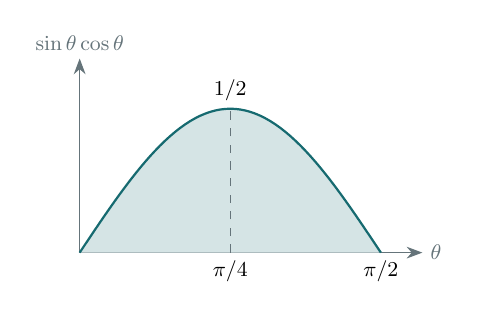
\begin{tikzpicture}[scale=.85,transform shape]
\draw[axis](0,0)--(5.12,0)node[right]{$\theta$};
\draw[axis](0,0)--(0,2.9)node[above]{$\sin\theta\cos\theta$};
\begin{scope}[x=.05cm,y=4.3cm]
\fill[accent!18](0,0)--plot[domain=0:90,samples=61](\x,{sin(\x)*cos(\x)})--cycle;
\draw[traj,domain=0:90,samples=61]plot(\x,{sin(\x)*cos(\x)});
\end{scope}
\node[below]at(2.25,0){$\pi/4$};
\node[below]at(4.5,0){$\pi/2$};
\draw[guide](2.25,0)--(2.25,2.15);
\node[above]at(2.25,2.15){$1/2$};
\end{tikzpicture}
\figcaption{变图热3.1V8\quad 方向积分的极角权重包含固体角和法向投影}
\end{minipage}\end{center}
\end{enumerate}

\clearpage

\pdfbookmark[2]{第 2 题 氯气分子反应冲量导致玻璃板偏转}{q2}

\section*{第 2 题\quad 氯气分子反应冲量导致玻璃板偏转}

质量$m$的均匀薄玻璃板宽$2b$、高$c$，由两根等长细线悬挂；每根线长$2a$，上、下悬点的水平间距均为$2a$，两下悬点关于板的竖直中心轴对称。两表面的半面分别对称涂活泼金属：正面左半、背面右半。装置处在压强$p$的氯气中，每个氯气分子遇涂层发生反应的概率为$q<1$，反应分子被吸收，其余分子与表面完全弹性碰撞。两侧密度相同，反应引起的气压下降忽略。求玻璃板绕竖直中心轴的小平衡转角$\alpha$。细线质量及扭转弹性忽略。

\begin{center}\begin{minipage}{0.96\linewidth}\centering\begin{tikzpicture}[x=1cm,y=1cm,font=\small,every node/.append style={align=center}]\draw[object] (-1.8,3.6)--(1.8,3.6);\draw[object] (-1.8,3.6)--(-1.8,0);\draw[object] (1.8,3.6)--(1.8,0);\fill[accent!25] (-2.5,-1.4) rectangle(0,0);\draw[object] (-2.5,-1.4) rectangle(2.5,0);\draw[guide] (0,3.9)--(0,-1.7);\draw[<->] (-1.8,4.1)--(1.8,4.1) node[midway,above]{$2a$};\node[left] at (-1.8,1.8){$2a$};\draw[<->] (-2.5,-1.8)--(2.5,-1.8) node[midway,below]{$2b$};\node[right] at (2.5,-.7){$c$};\node at (-1.2,-.7){正面涂层};\node at (1.25,-.7){背面涂层};\end{tikzpicture}\figcaption{图 热3.2　正面左半、背面右半涂层；两下悬点距中心轴均为$a$。}\end{minipage}\end{center}

\Needspace{5\baselineskip}

\pdfbookmark[3]{题型定位}{q2-h0}

\subsection*{题型定位}

先用分子冲量求涂层的动量通量，再用两个半面的力偶与悬线的恢复力矩求平衡角。

\Needspace{5\baselineskip}

\pdfbookmark[3]{知识点}{q2-h1}

\subsection*{知识点}

入射频率按法向速率 $u$ 加权，单次冲量与 $u$ 成正比。反射和吸收的冲量分别为 $2m_cu$ 和 $m_cu$。恒定反应概率 $q$ 使涂层获得的动量通量为 $(1-q/2)p$。下悬点移动弦长 $2a\sin(\alpha/2)$，线长 $2a$ 给 $\beta=\alpha/2$。


\Needspace{5\baselineskip}

\pdfbookmark[3]{物理图像}{q2-h2}

\subsection*{物理图像}

解图热3.2A中，左半和右半的差压力反向，顺时针力矩相加。解图热3.2B的 $SC$ 为下悬点的水平位移，水平张力的恢复力矩为逆时针。解图热3.2C中，板转动后下悬点由 $C_0$ 升到 $C$，重力势能随转角增加。

\Needspace{5\baselineskip}

\pdfbookmark[3]{解题入口}{q2-h3}

\subsection*{解题入口}

分别算反应吸收和弹性反射对 $p'$ 的贡献。差压力乘半面面积 $bc$，再乘两支力的距离 $b$，得气体力矩。由下悬点的弦长求线的倾角，用 $2N\cos\beta=mg$ 化去张力 $N$，最后在平衡式中取小角近似。


\Needspace{5\baselineskip}

\pdfbookmark[3]{标准解法}{q2-h4}

\subsection*{标准解法}

先算涂层改变了多少法向冲量。入射分子的法向速率为$|v_n|$，弹性反射传给板的冲量为$2m_c|v_n|$，吸收为$m_c|v_n|$。反应概率$q$与速度无关，碰撞通量相同，故
\[p'=(1-q)p+\frac q2p=\left(1-\frac q2\right)p,\qquad\Delta p=p-p'=\frac{qp}{2}.\]
\begin{center}\begin{minipage}{0.96\linewidth}\centering\begin{tikzpicture}[x=1cm,y=1cm,font=\small,every node/.append style={align=center}]\draw[object] (-2.5,0)--(2.5,0);\draw[accent,line width=3pt] (-2.5,.07)--(0,.07);\draw[warm,line width=3pt] (0,-.07)--(2.5,-.07);\draw[guide] (0,-1.5)--(0,1.5);\draw[force] (-1.25,-1.2)--(-1.25,-.1) node[pos=0,below]{$\Delta pbc$};\draw[force] (1.25,1.2)--(1.25,.1) node[pos=0,above]{$\Delta pbc$};\draw[<->] (0,.6)--(1.25,.6) node[midway,above]{$b/2$};\node[above] at (-2.8,1.2){俯视};\end{tikzpicture}\figcaption{解图 热3.2A　两个压强差作用在半面中心，形成同向转矩的力偶。}\end{minipage}\end{center}
解图热3.2A的俯视图中，正面左半和背面右半的压强差方向相反，形成力偶。每个半面面积$bc$，合力作用线过半面中心，离中心轴$b/2$。两力矩相加：
\[\tau_{\rm gas}=2(\Delta p\,bc)\frac b2=\frac12qp b^2c.\]
\textbf{细线的几何恢复力矩。} 两下悬点距轴均为$a$，转角$\alpha$后相对上悬点的水平偏移
\[d=2a\sin(\alpha/2)\simeq a\alpha.\]
每根线长$2a$，倾角$\beta$满足$\sin\beta=d/(2a)=\sin(\alpha/2)$，所以小角下$\beta\simeq\alpha/2$。竖直平衡给$2N\cos\beta=mg$。
\begin{center}\begin{minipage}{0.96\linewidth}\centering\begin{tikzpicture}[x=1cm,y=1cm,font=\small]
\draw[guide] (-2.5,0)--(2.6,0);
\draw[object] ({-2*cos(30)},{2*sin(30)})--({2*cos(30)},{-2*sin(30)});
\fill (0,0) circle(1.5pt) node[below left] {$O$};
\coordinate (C) at ({2*cos(30)},{-2*sin(30)});
\coordinate (S) at (2,0);
\draw[motion] (C)--(S) node[midway,right] {$N\sin\beta$};
\draw[motion] ({-2*cos(30)},{2*sin(30)})--(-2,0)
 node[midway,left] {$N\sin\beta$};
\fill (C) circle(1.5pt) node[below] {$C$};
\fill (S) circle(1.5pt) node[above right] {$S$};
\draw[<->] (0,.5)--(2,.5) node[midway,above] {$a$};
\draw (.85,0) arc(0:-30:.85);
\node at (1.04,-.23) {$\alpha$};
\node[align=left] at (-2.6,-.85) {$SC=d$\\顺时针偏转\\逆时针恢复};
\node[below] at (0,-1.6) {俯视；虚线为未偏转位置，示意角度放大};
\end{tikzpicture}\figcaption{解图 热3.2B　小角下$d\simeq a\alpha$、$\beta\simeq\alpha/2$；张力提供恢复转矩。}\end{minipage}\end{center}
解图热3.2B标出下悬点的水平偏移，悬线倾角另见解图热3.2C；水平张力的力臂为$a\cos(\alpha/2)$，两根线的恢复力矩为
\[\tau_{\rm res}=2Na\sin\beta\cos(\alpha/2)\simeq Na\alpha\simeq\frac12mga\alpha.\]
令两力矩大小相等，得
\result{\alpha=\frac{qpb^2c}{mga},\qquad\alpha\ll1.}
偏转也使玻璃板抬高。细线竖直投影为 $\sqrt{4a^2-d^2}$，板升高 $\Delta z\simeq d^2/(4a)=a\alpha^2/4$，于是 $\dd(mg\Delta z)/\dd\alpha=mga\alpha/2$。两式都把恢复系数联系到下悬点的横移距离。改变涂层位置时，按各半面的差压重新求合力和力矩。
\subsubsection*{用法向动量通量展开涂层压强}
设氯气单分子质量为$m_c$，入射法向速率$u>0$的一维概率密度为$g(u)$。
单位面积、单位时间到达的相应分子数为$nu g(u)\dd u$；
再乘单次法向冲量，弹性反射与吸收两种压强分别为
\[
p_{\rm el}=2nm_c\int_0^\infty u^2g(u)\dd u=p,\qquad
p_{\rm abs}=nm_c\int_0^\infty u^2g(u)\dd u=\frac p2.
\]
题设$q$与速度无关，所以吸收反应和未反应反射的贡献可分别写为
\[
p'_{\rm react}=\frac q2p,\qquad
p'_{\rm refl}=(1-q)p.
\]
二者相加得到$p'=(1-q/2)p$。
容器中的气体状态压强为 $p$。在涂层上，有些分子被吸收，每次只传递弹性反射时一半的冲量。因此，气体传给涂层的法向动量通量为 $p'$。

解图热3.2A中，左半面差压力向上、右半面向下，净力相消，转矩同为顺时针。
每个半面的力是$\Delta pbc$，两作用线相距$b$，
两支差压力等大反向，直接用其中一支力乘两力作用线之间的距离 $b$，得到 $\tau_{\rm gas}=(\Delta pbc)b$。
解图热3.2B按同一俯视方向画成顺时针偏转，
两根张力的水平分量均提供逆时针恢复转矩；两图采用同一俯视方向，恢复转矩与气体力矩相反。

\subsubsection*{悬线的竖直几何和小角近似的精度}
解图热3.2C单独画一根悬线所在的竖直平面。
U为固定上悬点，$C_0$为未转动时下悬点，C为转后的下悬点，
S是U在C所在水平面上的垂直投影。
$SC=d$是俯视图中同一弦长，而US为悬线的竖直投影。

\begin{center}\begin{minipage}{0.96\linewidth}\centering
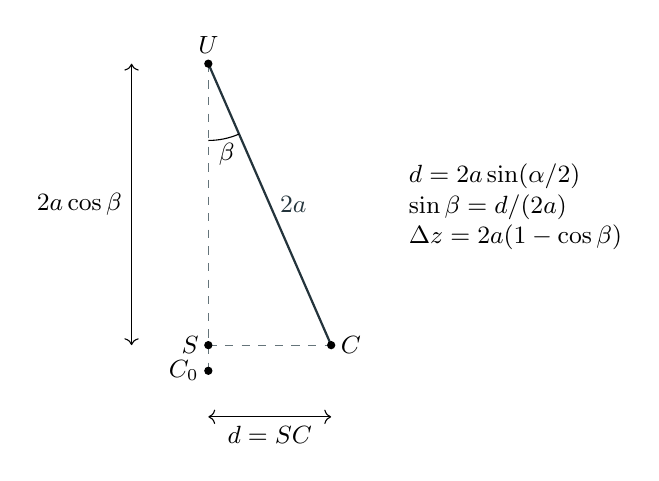
\begin{tikzpicture}[x=1.3cm,y=1.3cm,font=\small]
\coordinate (U) at (0,3);
\coordinate (C) at (1.2,{3-sqrt(9-1.44)});
\coordinate (S) at (0,{3-sqrt(9-1.44)});
\draw[guide] (U)--(0,0);
\draw[object] (U)--(C) node[midway,right] {$2a$};
\draw[guide] (S)--(C);
\draw[<->] (-.75,{3-sqrt(9-1.44)})--(-.75,3)
 node[midway,left] {$2a\cos\beta$};
\draw[<->] (0,-.45)--(1.2,-.45) node[midway,below] {$d=SC$};
\draw (0,2.25) arc(-90:-66.4218:.75);
\node at (.18,2.12) {$\beta$};
\fill (U) circle(1.5pt) node[above] {$U$};
\fill (0,0) circle(1.5pt) node[left] {$C_0$};
\fill (C) circle(1.5pt) node[right] {$C$};
\fill (S) circle(1.5pt) node[left] {$S$};
\node[align=left] at (3,1.6) {$d=2a\sin(\alpha/2)$\\$\sin\beta=d/(2a)$\\$\Delta z=2a(1-\cos\beta)$};
\end{tikzpicture}
\figcaption{解图 热3.2C　一根悬线的竖直截面；偏转使玻璃板升高，重力势能给恢复转矩。}
\end{minipage}\end{center}
在$0\le\alpha<\pi$的几何支上，$\beta=\alpha/2$。
不先作小角近似，由竖直平衡$N=mg/[2\cos(\alpha/2)]$代回，
\[
\tau_{\rm res}
=2Na\sin(\alpha/2)\cos(\alpha/2)
=mga\sin(\alpha/2)
=\frac12mga\alpha+O(\alpha^3).
\]
势能法同样给
\[
\Delta z=2a[1-\cos(\alpha/2)],\qquad
\frac{\dd(mg\Delta z)}{\dd\alpha}=mga\sin(\alpha/2).
\]
小角恢复力矩的系数由线长 $2a$ 和悬点半间距 $a$ 共同确定。其中 $1/2$ 来自悬线倾角与玻璃板转角的对应关系。
若仍采用各向同性气体、恒定$q,p$及相同涂层面积的模型，
气体力偶大小与板的水平转角无关，可进一步写
\[
\sin\frac\alpha2=\frac{qpb^2c}{2mga},\qquad
\alpha=2\arcsin\!\left(\frac{qpb^2c}{2mga}\right).
\]
小角近似要求$qpb^2c/(mga)\ll1$，
在这一范围内展开正弦式可得线性转角。若角度较大，按给定气体模型使用正弦关系，并在悬线有正竖直投影的几何支上求解。


\Needspace{5\baselineskip}

\pdfbookmark[3]{关键洞察}{q2-h5}

\subsection*{关键洞察}

状态压强 $p$ 相同，板面是否吸收分子决定每次碰撞给板多少动量。恒定 $q$ 可在积分外加权，速度依赖的 $q(u)$ 放在动量通量积分内。恢复力矩由悬线几何决定，受力半面的位置则给气体力矩的力臂。

\Needspace{5\baselineskip}

\pdfbookmark[3]{易错点}{q2-h6}

\subsection*{易错点}

\begin{itemize}
\item 两半面的合力为零，各力对中心轴的同向力矩相加。每支力的力臂是 $b/2$，两作用线之间的距离为 $b$。
\item 图中的玻璃板转角为 $\alpha$，悬线倾角为 $\beta=\alpha/2$，并由两线共同承担 $mg$。
\item 板的升高量是悬线竖直投影的缩短量。气体力矩、玻璃板偏转和恢复力矩均在同一俯视方向上判断。
\end{itemize}

\Needspace{5\baselineskip}

\pdfbookmark[3]{课堂讲解建议}{q2-h7}

\subsection*{课堂讲解建议}

先在解图热3.2A上还原两侧四个半面的压力。让学生在抵消公共的 $p$ 后，沿剩下的两支差力各自画力臂，说明合力为零仍可产生力偶。

从解图热3.2B的弦长确定 $\beta$，再用解图热3.2C的升高量说明为何重力能使板回转。比较张力法与势能法的系数 $mga/2$，再改用变图热3.2V2的单侧涂层，分别画出引起质心平移和板绕轴偏转的力。

\Needspace{5\baselineskip}

\pdfbookmark[3]{变式训练}{q2-h8}

\subsection*{变式训练}

\begin{enumerate}
\item 将 $q$ 变为 $2q$，仍令 $2q\leq1$。气体力矩 $\tau_{\rm gas}=qpb^2c/2$ 随之加倍。变图热3.2V1的纵坐标 $\hat\tau=\tau_{\rm gas}/(mga)$，沿正弦曲线分别得到
\[
\sin(\alpha_1/2)=\hat\tau,\qquad
\sin(\alpha_2/2)=2\hat\tau .
\]
若两角都很小，$\alpha_2\simeq2\alpha_1$。有限角对应 $\alpha_2=2\arcsin(2\hat\tau)$，此式取 $2\hat\tau<1$。
\begin{center}\begin{minipage}{.98\linewidth}\centering
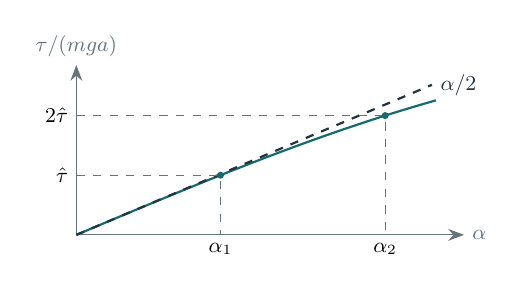
\begin{tikzpicture}[scale=.85,transform shape]
\begin{scope}[x=3.2cm,y=2.7cm]
\draw[axis](0,0)--(1.81,0)node[right]{$\alpha$};
\draw[axis](0,0)--(0,.94)node[above]{$\tau/(mga)$};
\draw[traj,domain=0:1.68,samples=66]plot(\x,{sin(deg(\x/2))});
\draw[object,dashed](0,0)--(1.66,.83)node[right]{$\alpha/2$};
\draw[guide](0,.33)--(.673,.33)--(.673,0);
\draw[guide](0,.66)--(1.442,.66)--(1.442,0);
\fill[accent](.673,.33)circle(1.5pt);
\fill[accent](1.442,.66)circle(1.5pt);
\node[left]at(0,.33){$\hat\tau$};\node[left]at(0,.66){$2\hat\tau$};
\node[below]at(.673,0){$\alpha_1$};\node[below]at(1.442,0){$\alpha_2$};
\end{scope}
\end{tikzpicture}
\figcaption{变图热3.2V1\quad 气体力矩加倍时，沿正弦恢复曲线找到两个平衡角}
\end{minipage}\end{center}
\item 只涂正面左半。变图热3.2V2的净力大小为 $F=\Delta pbc$，作用线离中心 $b/2$，所以 $\tau_{\rm gas}=Fb/2$。设板中心沿差力方向平移 $Y$，保持 $Y\ll 2a$、$\alpha\ll1$。两下悬点的横向移动分别约为 $Y+a\alpha$ 和 $Y-a\alpha$。每根线的恢复力为该位移乘 $mg/(4a)$，相加和取矩分别得到
\[
F=\frac{mg}{2a}Y,\qquad \frac{Fb}{2}=\frac{mga}{2}\alpha.
\]
于是 $Y=2aF/(mg)$，转角为对置涂层时的一半，还需 $F/(mg)\ll1$ 来保证平移近似。
\begin{center}\begin{minipage}{.98\linewidth}\centering
\begin{tikzpicture}[scale=.85,transform shape]
\draw[object](-2.8,0)--(2.8,0);
\draw[accent,line width=2.4pt](-2.8,.08)--(0,.08);
\draw[guide](0,-1.48)--(0,1.9);
\fill(0,0)circle(1.5pt)node[below right]{$O$};
\draw[force](-1.4,-1.35)--(-1.4,-.1)node[pos=0,below]{$F$};
\draw[<->](-1.4,.6)--(0,.6)node[midway,above]{$b/2$};
\draw[motion](.65,.1)--(.65,1.4)node[above]{$Y$};
\draw[force](1.22,.32)arc(28:-50:1.3)node[below right]{$\tau_{\rm gas}$};
\node[above]at(-2.13,1.26){俯视};
\end{tikzpicture}
\figcaption{变图热3.2V2\quad 单半面只留一支差力，在中心处等效为一支净力和一个力矩}
\end{minipage}\end{center}
\item 令压强 $p(t)$ 缓慢下降。板能近似保持各时刻的静态平衡，故 $\alpha(t)=qb^2cp(t)/(mga)$。变图热3.2V3取指数下降作为示例，归一化角度与压强轨迹重合。若压强变化的时间与板的运动时间相近，可用小角方程
\[
I\ddot\alpha+\Gamma\dot\alpha+\frac{mga}{2}\alpha
=\frac{qb^2c}{2}p(t)
\]
求角度随时间的变化，其中 $I$ 为玻璃板绕竖直中心轴的转动惯量，$\Gamma$ 为采用线性阻尼模型时的系数。
\begin{center}\begin{minipage}{.98\linewidth}\centering
\begin{tikzpicture}[scale=.85,transform shape]
\draw[axis](0,0)--(6.1,0)node[right]{$t$};
\draw[axis](0,0)--(0,3.0)node[above]{归一化量};
\draw[traj,domain=0:5.6,samples=75]plot(\x,{2.55*exp(-.26*\x)})node[right]{$p/p_0$};
\draw[object,dashed,domain=0:5.6,samples=75]plot(\x,{2.55*exp(-.26*\x)});
\node[above right]at(1.7,1.87){$\alpha/\alpha_0$ 与实线重合};
\node[left]at(0,2.55){$1$};
\end{tikzpicture}
\figcaption{变图热3.2V3\quad 准静态压强衰减时，归一化后的平衡角随压强同步下降}
\end{minipage}\end{center}
\item 改用半径 $R$ 的圆盘，悬点半距仍为 $a$，线长为 $2a$。变图热3.2V4的右半圆，在离中心轴水平距离 $x$ 处取高 $2\sqrt{R^2-x^2}$ 的窄条。对条形压力取矩，
\[
\int_{\text{半圆}}x\,\dd A
=\int_0^R2x\sqrt{R^2-x^2}\,\dd x=\frac{2R^3}{3}.
\]
两涂层的差压均为 $qp/2$，总转矩为 $2qpR^3/3$，由小角恢复系数 $mga/2$ 得 $\alpha=4qpR^3/(3mga)$。
\begin{center}\begin{minipage}{.98\linewidth}\centering
\begin{tikzpicture}[scale=.85,transform shape]
\fill[accent!18](0,-1.8)arc(-90:90:1.8)--cycle;
\draw[object](0,0)circle(1.8);
\draw[axis](-2.34,0)--(2.65,0)node[right]{$x$};
\draw[axis](0,-2.1)--(0,2.46)node[above]{$y$};
\begin{scope}\clip(0,0)circle(1.8);\fill[warm!33](1.05,-1.8)rectangle(1.19,1.8);\end{scope}
\draw[<->](0,-2.15)--(1.12,-2.15)node[midway,below]{$x$};
\draw[guide](1.12,-1.41)--(1.12,-2.11);
\node[right]at(1.25,1.3){条宽 $\dd x$};
\node[left]at(-1.45,1.66){圆半径 $R$};
\end{tikzpicture}
\figcaption{变图热3.2V4\quad 圆形涂层可取平行于转轴投影线的窄条，逐条乘到轴的力臂}
\end{minipage}\end{center}
\item 悬线长改为 $l$，上、下悬点半距均为 $a$。转角很小时，下悬点弦长 $d\simeq a\alpha$。变图热3.2V5的竖直投影为 $\sqrt{l^2-d^2}$，展开得到
\[
\Delta z=l-\sqrt{l^2-d^2}\simeq\frac{a^2\alpha^2}{2l},\qquad
\tau_{\rm res}\simeq\frac{mga^2}{l}\alpha .
\]
平衡角为 $\tau_{\rm gas}l/(mga^2)$。代入 $l=2a$ 还原系数 $mga/2$。
\begin{center}\begin{minipage}{.98\linewidth}\centering
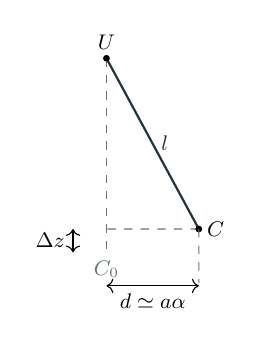
\begin{tikzpicture}[scale=.85,transform shape]
\coordinate (U) at(0,2.9);
\coordinate (C) at (1.38,{2.9-sqrt(2.9^2-1.38^2)});
\draw[object](U)--(C)node[midway,right]{$l$};
\draw[guide](U)--(0,0)node[below]{$C_0$};
\draw[guide](C)--(0,{2.9-sqrt(2.9^2-1.38^2)});
\fill (U) circle(1.45pt) node[above]{$U$};
\fill (C) circle(1.45pt) node[right]{$C$};
\draw[<->](-.5,0)--(-.5,{2.9-sqrt(2.9^2-1.38^2)})node[midway,left]{$\Delta z$};
\draw[guide](C)--(1.38,-.46);
\draw[<->](0,-.5)--(1.38,-.5)node[midway,below]{$d\simeq a\alpha$};
\end{tikzpicture}
\figcaption{变图热3.2V5\quad 固定横移弦长时，改变悬线长度会改变板的升高量}
\end{minipage}\end{center}
\item 正面与背面都只涂左半。变图热3.2V6的左对箭头等大，均由涂层上的 $p'$ 产生，右对箭头均由弹性反射的 $p$ 产生。两侧对应位置的压力等大反向。逐点相加为零，因而总合力和对中心轴的力矩均为零。
\begin{center}\begin{minipage}{.98\linewidth}\centering
\begin{tikzpicture}[scale=.85,transform shape]
\draw[object](-2.75,0)--(2.75,0);
\draw[accent,line width=2.4pt](-2.75,.09)--(0,.09);
\draw[warm,line width=2.4pt](-2.75,-.09)--(0,-.09);
\draw[guide](0,-1.56)--(0,1.56);
\foreach \x/\len/\labelp in {-1.35/.79/$p'$,1.35/1.22/$p$}{
\draw[force](\x,{\len+.15})--(\x,.18)node[pos=0,above]{\labelp};
\draw[force](\x,{-\len-.15})--(\x,-.18)node[pos=0,below]{\labelp};
}
\node[above]at(-2.4,1.37){俯视};
\end{tikzpicture}
\figcaption{变图热3.2V6\quad 上下对应位置的压力相等，两半面均逐点抵消}
\end{minipage}\end{center}
\item 令反应概率为法向速率的函数 $q(u)$。达到面元的速率谱为 $nu g(u)\dd u$，每次反应使传给板的冲量少 $m_cu$，于是
\[
\Delta p=nm_c\int_0^\infty q(u)u^2g(u)\,\dd u .
\]
变图热3.2V7用同一尺度画出动量通量密度和乘概率后的密度。两条曲线下面积之比是按 $u^2g(u)$ 加权的有效概率，故 $\Delta p=(p/2)q_{\rm eff}$。当各速率的概率同为 $q$，面积比就是 $q$。
\begin{center}\begin{minipage}{.98\linewidth}\centering
\begin{tikzpicture}[scale=.85,transform shape]
\begin{scope}[x=1.52cm,y=3.75cm]
\draw[axis](0,0)--(4.1,0)node[right]{$u/\sigma$};
\draw[axis](0,0)--(0,.8)node[above]{动量通量谱尺度};
\draw[traj,domain=0:3.8,samples=94]plot(\x,{\x^2*exp(-\x*\x/2)});
\draw[object,dashed,domain=0:3.8,samples=94]plot(\x,{(.2+.6*\x^2/(1+\x^2))*\x^2*exp(-\x*\x/2)});
\node[above right]at(1.62,.655){$u^2g(u)$};
\node[below right]at(1.63,.40){$q(u)u^2g(u)$};
\end{scope}
\end{tikzpicture}
\figcaption{变图热3.2V7\quad 用动量通量谱给反应概率加权，虚线以一个变速率的概率为例}
\end{minipage}\end{center}
\item 保持气体各向同性和恒定的 $p,q$，用完整恢复式求角。令 $\eta=qpb^2c/(2mga)$。变图热3.2V8的水平线在 $0\leq\eta<1$ 处与 $\sin(\alpha/2)$ 相交，给 $\alpha=2\arcsin\eta$。图的右端 $\alpha=\pi$ 对应悬线竖直投影趋零。$\eta\ll1$ 时 $\alpha\simeq2\eta$。若板面反应改变气体力偶的角度依赖，可重新画 $\tau_{\rm gas}(\alpha)/(mga)$ 与此恢复曲线求交。
\begin{center}\begin{minipage}{.98\linewidth}\centering
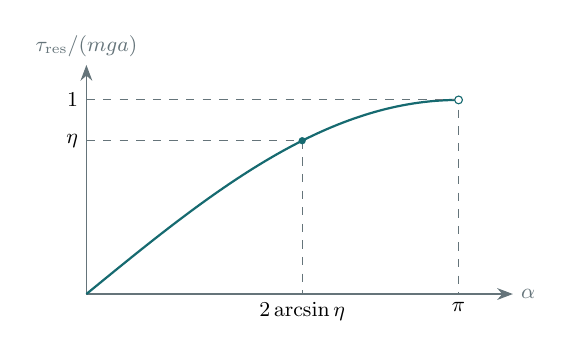
\begin{tikzpicture}[scale=.85,transform shape]
\begin{scope}[x=1.77cm,y=2.9cm]
\draw[axis](0,0)--(3.6,0)node[right]{$\alpha$};
\draw[axis](0,0)--(0,1.18)node[above]{$\tau_{\rm res}/(mga)$};
\draw[traj,domain=0:3.14159,samples=85]plot(\x,{sin(deg(\x/2))});
\draw[guide](0,.79)--(1.82162,.79)--(1.82162,0);
\fill[accent](1.82162,.79)circle(1.55pt);
\draw[guide](0,1)--(3.14159,1)--(3.14159,0);
\draw[accent,fill=white](3.14159,1)circle(1.65pt);
\node[left]at(0,.79){$\eta$};
\node[left]at(0,1){$1$};
\node[below]at(1.82162,0){$2\arcsin\eta$};
\node[below]at(3.14159,0){$\pi$};
\end{scope}
\end{tikzpicture}
\figcaption{变图热3.2V8\quad 正弦曲线给有限倾角的平衡支，末端空心点对应竖直投影趋零}
\end{minipage}\end{center}
\end{enumerate}

\clearpage

\pdfbookmark[2]{第 3 题 隔板推动试管后的最终速度}{q3}

\section*{第 3 题\quad 隔板推动试管后的最终速度}

真空中质量$M$的试管由质量$m$的隔板等分，封闭的下半管内装有$n$ mol、温度$T$、摩尔质量$\mu$的单原子理想气体。初始三者均静止。放开隔板后，它无摩擦地向管口移动，离开管口后气体才逸出。忽略重力及三者间热交换，隔板离管前的气体过程按准静态绝热处理。估算全部气体逸出后试管的最终速度，说明逸出阶段所用的分子冲量近似。

\begin{center}\begin{minipage}{0.96\linewidth}\centering\begin{tikzpicture}[x=1cm,y=1cm,font=\small,every node/.append style={align=center}]\draw[object] (0,3)--(0,0)--(2,0)--(2,3);\fill[accent!12] (0,0) rectangle(2,1.5);\draw[object,line width=2pt] (0,1.5)--(2,1.5);\node at (1,.7){$n,T,V$};\node[right] at (2.2,1.5){隔板$m$};\node[right] at (2.2,.2){试管$M$};\end{tikzpicture}\figcaption{图 热3.3　隔板初位于管长的一半；封闭气体在下半管。}\end{minipage}\end{center}

\Needspace{5\baselineskip}

\pdfbookmark[3]{题型定位}{q3-h0}

\subsection*{题型定位}

以隔板离管为分界，先算封闭气体膨胀带动试管的速度，再估算开口逸出给试管的额外反冲。

\Needspace{5\baselineskip}

\pdfbookmark[3]{知识点}{q3-h1}

\subsection*{知识点}

封闭阶段用单原子气体 $TV^{2/3}$ 恒定求 $T_f$，用能量和动量确定共同后退速度。开口阶段在以 $-u_1$ 匀速运动的惯性系中处理一次碰底冲量。方均根法向速率为 $\sqrt{RT_f/\mu}$，平均绝对法向速率是它的 $\sqrt{2/\pi}$ 倍。


\Needspace{5\baselineskip}

\pdfbookmark[3]{物理图像}{q3-h2}

\subsection*{物理图像}

解图热3.3A中，隔板向管口，试管与气体整体向后。解图热3.3B标出初始朝底的一批分子，各给底面一次反射冲量，方向沿管向后。解图热3.3C的阴影为这批分子的初始法向速度，冲量由这半边概率密度乘 $|v_x|$ 求得。

\Needspace{5\baselineskip}

\pdfbookmark[3]{解题入口}{q3-h3}

\subsection*{解题入口}

先求 $T_f=2^{-2/3}T$ 和释放的内能 $3nR(T-T_f)/2$。在共同后退模型中，以 $mv_p=Bu_1$ 消去 $v_p$。离管后固定第二段的惯性系，先数朝底的 $nN_A/2$ 个分子，乘单分子反射冲量，再比较代表速率与分布平均的系数。


\Needspace{5\baselineskip}

\pdfbookmark[3]{标准解法}{q3-h4}

\subsection*{标准解法}

\textbf{隔板尚未离管。} 初始封闭气体体积记为$V$，隔板到管口时体积$2V$。按所给准静态绝热模型，$\gamma=5/3$，
\[TV^{2/3}=T_f(2V)^{2/3},\qquad T_f=2^{-2/3}T.\]
在共同后退的估算中，把试管及气体合并为质量$B=M+n\mu$的部分，后退速度大小$u_1$，隔板向前速度$v_p$。系统无外力，初始总动量零：
\[mv_p=Bu_1.\]
气体内能减少转为上述两部分的定向动能，
\[\frac32nR(T-T_f)=\frac12mv_p^2+\frac12Bu_1^2
=\frac{B(B+m)}{2m}u_1^2.\]
\begin{center}\begin{minipage}{0.96\linewidth}\centering\begin{tikzpicture}[x=1cm,y=1cm,font=\small,every node/.append style={align=center}]
\draw[object] (0,3)--(0,0)--(2.8,0)--(2.8,3);
\fill[accent!12] (0,0) rectangle (2.8,2.94);
\draw[guide] (0,1.5)--(2.8,1.5);
\node[left] at (-.1,1.5) {初始隔板位置};
\draw[object,line width=2pt] (0,3)--(2.8,3);
\node at (1.4,1) {$n,T_f,2V$\\$T_f=2^{-2/3}T$};
\node[right] at (3,3) {隔板$m$：到达管口};
\node[right] at (3,.2) {试管$M$};
\draw[motion] (4.5,1.8)--(4.5,2.8) node[right,midway] {$v_p$};
\draw[motion] (-2,1.2)--(-2,.2) node[left,midway] {$u_1$};
\node[above] at (1.4,3.7) {离管前：$V\longrightarrow 2V$};
\end{tikzpicture}\figcaption{解图 热3.3A\quad 隔板到达管口前，气体体积为$2V$、温度为$T_f$；$v_p$向上，$u_1$向下。}\end{minipage}\end{center}
解图热3.3A中，隔板的速度$v_p$向上，试管与尚未逸出气体的速度$u_1$向下。两部分总动量为零，故$mv_p=Bu_1$；能量式中的$B$也包括气体质量。隔板离管后转入解图热3.3B的开口逸出过程，气体质量开始减少。

消去$v_p$得
\[u_1=\sqrt{\frac{3mnR(T-T_f)}{(M+n\mu)(M+n\mu+m)}}.\]
\textbf{离管后的代表速率估算。} 从离管瞬间的状态出发，取以 $-u_1$ 匀速运动的惯性系。图中散开前朝底运动的半数分子各碰底一次，以一维方均根热速代表各分子的法向速率：
\[m_0=\frac{\mu}{N_A},\qquad v_{x,\rm rms}=\sqrt{\frac{kT_f}{m_0}}=\sqrt{\frac{RT_f}{\mu}}.\]
单次弹性碰撞冲量$2m_0v_{x,\rm rms}$，半数分子总冲量
\[P_{\rm rms}=\frac{nN_A}{2}\,2\frac\mu{N_A}\sqrt{\frac{RT_f}{\mu}}
=n\sqrt{\mu RT_f}.\]
\begin{center}\begin{minipage}{0.96\linewidth}\centering\begin{tikzpicture}[x=1cm,y=1cm,font=\small,every node/.append style={align=center}]\draw[object] (0,3)--(0,0)--(2,0)--(2,3);\draw[motion] (.5,1.7)--(.5,.15);\draw[motion] (.8,.2)--(.8,3.6);\draw[motion] (1.5,1.5)--(1.5,3.6);\node[left] at (0,.7){撞底};\node[right] at (2,2){向上者直接出管};\draw[force] (3,.8)--(3,-.1) node[right]{$P$};\end{tikzpicture}\figcaption{解图 热3.3B　一次碰底的代表速率模型：向下分子反射，给管底向后的冲量。}\end{minipage}\end{center}
于是该代表速率模型给出$u_2=P_{\rm rms}/M$，试管沿背离管口的方向运动：
\result{u\simeq\sqrt{\frac{3mnRT(1-2^{-2/3})}{(M+n\mu)(M+n\mu+m)}}
+\frac{n}{2^{1/3}M}\sqrt{\mu RT}.}
\textbf{统计平均及适用条件。} 第二项用了代表速率。改用初始麦克斯韦一维分布$g(v_x)$用于一次碰底模型，得
\[P=2nN_A m_0\int_{-\infty}^{0}|v_x|g(v_x)\dd v_x
=n\mu\langle|v_x|\rangle
=n\sqrt{\frac{2\mu RT_f}{\pi}}.\]
因此固定底面的一次碰撞平均会把第二项乘以$\sqrt{2/\pi}$。在 $n\mu\ll M$ 且一次碰底模型适用时，底面速度的变化相对热速很小，分子间后续碰撞也在本估算中略去。封闭阶段采用题设的准静态绝热假定。
\subsubsection*{先交代系统、参考系和两段的近似层次}
解图热3.3A以管口方向为正，离管前试管与隔板均可运动。
外界为真空，整个系统所受的外界压力功为零。气体在系统内部对隔板和管底做功。
封闭阶段的气体内能减少，可转为系统各部分的宏观定向动能；
把气体整体后退的动能与气体分子的无规则热运动内能分开计算。

第一段采用的估算还把气体整体后退速度视作与试管相同。
因此共同后退的质量写为 $B=M+n\mu$。准静态绝热式给出热运动的温度变化，共同后退是假定的宏观运动。若气体内部各处有不同的宏观速度，气体的整体动量和动能分别按局部速度和局部速度平方积分。

第二段改用一个以离管瞬间速度$-u_1$匀速运动的惯性系。
试管相对该系从静止开始，受到向后的分子冲量后速度变成 $-u_2$。参考系一直以 $-u_1$ 匀速移动。
变回初始实验室系，试管速度为$-(u_1+u_2)$，
所以最后所加的是两个同方向后退速率。
逸出期间还忽略分子间再碰撞、出管分子与隔板的后续碰撞，
以及管底反冲对碰底数目和相对入射速率的改变。
这些近似决定一次冲量模型所保留的过程。

\subsubsection*{封闭膨胀的温度、动量与能量全部展开}
隔板从管长一半移动到管口，气体体积从$V$变为$2V$。
单原子气体的$C_V=3R/2,\gamma=5/3$，
因此$T_f/T=2^{-2/3}$，剩余内能为$3nRT_f/2$，
释放到定向运动中的能量为
\[
\Delta U_{\rm released}
=\frac32nRT(1-2^{-2/3}).
\]
共同后退模型中，动量式给$v_p=Bu_1/m$。
代入动能式时逐项为
\[
\frac12mv_p^2+\frac12Bu_1^2
=\frac{B^2}{2m}u_1^2+\frac B2u_1^2
=\frac{B(B+m)}{2m}u_1^2.
\]
所以
\[
u_1^2=\frac{3mnRT(1-2^{-2/3})}
{(M+n\mu)(M+n\mu+m)}
=\frac{3(2^{2/3}-1)mnRT}
{2^{2/3}(M+n\mu)(M+n\mu+m)}.
\]
两种写法等价。动量 $Bu_1$ 和宏观动能 $Bu_1^2/2$ 中的后退质量均包括试管和气体。由 $v_p=Bu_1/m$ 求得隔板速度，两者动量大小相等，定向动能之和等于内能减少量。

\subsubsection*{逐个分子冲量的计数与统计平均}
离管前的热运动近似各向同性，
\[
\langle v_x^2\rangle=\langle v_y^2\rangle
=\langle v_z^2\rangle=\frac13\langle v^2\rangle,\qquad
\langle v^2\rangle=\frac{3RT_f}{\mu}.
\]
法向是三个等价分量之一，方均根为 $\sqrt{RT_f/\mu}$，即三维方均根的一份 $1/\sqrt3$。
解图热3.3B的代表速率模型把初始向下的半数分子视为各碰底一次，
向上的半数直接出管。单分子质量为$\mu/N_A$，
反射给管底冲量$2(\mu/N_A)\sqrt{RT_f/\mu}$，
总数$nN_A/2$相乘时阿伏伽德罗常量恰好约去，
得到$n\sqrt{\mu RT_f}$。
这项反冲只改变试管速度，用 $P_{\rm rms}/M$ 得该模型的速度增量 $u_2$。

如果使用同一初始热运动的完整一维分布，
令$\sigma=\sqrt{RT_f/\mu}$、$w=v_x/\sigma$，
\[
g(v_x)=\frac{1}{\sqrt{2\pi}\sigma}
\exp\!\left(-\frac{v_x^2}{2\sigma^2}\right),\qquad
\int_{-\infty}^{0}g(v_x)\dd v_x=\frac12.
\]
解图热3.3C中只有负速率分量对应初始朝底运动的分子，
对这半边取 $|v_x|$ 积分，反映各次入射冲量同向叠加。

\begin{center}\begin{minipage}{0.96\linewidth}\centering
\begin{tikzpicture}[x=1.15cm,y=4cm,font=\small]
\draw[axis] (-3.3,0)--(3.5,0) node[right] {$w=v_x/\sigma$};
\draw[axis] (0,0)--(0,.55) node[above] {$h(w)$};
\fill[accent!15,domain=-3:0,samples=80]
 (-3,0)--plot (\x,{exp(-.5*\x*\x)/sqrt(2*pi)})--(0,0)--cycle;
\draw[traj,domain=-3:3,samples=110]
 plot (\x,{exp(-.5*\x*\x)/sqrt(2*pi)});
\node at (-1.45,.26) {朝底，概率$1/2$};
\node at (1.6,.26) {朝管口};
\node[below] at (0,0) {0};
\end{tikzpicture}
\figcaption{解图 热3.3C　初始法向速度分布；一次碰底总冲量对负半轴按$|v_x|$加权。}
\end{minipage}\end{center}
在固定底面、忽略后续碰撞的近似内，
\[
P_{\rm mean}
=2n\mu\int_{-\infty}^{0}|v_x|g(v_x)\dd v_x
=2n\mu\frac{\sigma}{\sqrt{2\pi}}
=n\sqrt{\frac{2\mu RT_f}{\pi}}.
\]
因此
\[
u_{2,\rm mean}
=\frac n{2^{1/3}M}\sqrt{\frac{2\mu RT}{\pi}},
\qquad
\frac{P_{\rm mean}}{P_{\rm rms}}=\sqrt{\frac2\pi}\simeq0.7979.
\]
这里统计的是有限一批分子各碰一次的总冲量，
故用单侧速度的一阶矩；稳态气压还要按单位时间到达次数加权，
才出现速度的二阶矩。这里的有限批次由各分子的单次冲量直接求和。

\subsubsection*{管底反冲与末态动能}
固定底面反射保留每个分子的速率。有限质量的试管受到反冲后获得动能，这部分能量由气体转移。若管底速度显著，分子的相对入射速度随时间改变，部分较慢的分子会追不上后退的底面。$n\mu/M\ll1$ 时，底面的速度改变量相对热速小，单次固定底面冲量可作首阶估算。

末态动量确定后，可用质心动能求最低所需能量。
在第二段所取惯性系，若管底获得后退动量P，气体最终总动量为$+P$，
则两者末态的总动能至少为
\[
K_{\rm min}=\frac{P^2}{2M}+\frac{P^2}{2n\mu}.
\]
在一次碰底模型中，忽略气体与离管隔板的后续交换，第二段可用的初始气体内能为 $3nRT_f/2$，故要求 $K_{\rm min}\leq3nRT_f/2$。代代表速率冲量 $P_{\rm rms}=n\sqrt{\mu RT_f}$，得到必要条件 $1+n\mu/M\le3$。实际剩余的热运动会继续占用这笔能量。代表速率与分布平均的估算均给出同一后退方向，速度增量的尺度为 $n\sqrt{\mu RT_f}/M$，区别在法向速率的选取。


\Needspace{5\baselineskip}

\pdfbookmark[3]{关键洞察}{q3-h5}

\subsection*{关键洞察}

准静态绝热给出温度随体积的变化，气体整体的后退速度在所用模型中与试管合并。一次碰底统计有限批次中每个分子的冲量，所用的一阶矩与稳态气压的二阶矩不同。管底反冲相对热速小的尺度是 $n\mu/M\ll1$。

\Needspace{5\baselineskip}

\pdfbookmark[3]{易错点}{q3-h6}

\subsection*{易错点}

\begin{itemize}
\item 封闭阶段的动量和宏观动能采用同一后退质量 $B=M+n\mu$。
\item 管底沿轴受冲量，采用一个速度分量的方均根。朝底的分子都向后传递动量，按绝对值统计。
\item 开口阶段的速度增量为冲量除试管质量 $M$。两段速度在同一初始实验室系中合成为后退速度。
\end{itemize}

\Needspace{5\baselineskip}

\pdfbookmark[3]{课堂讲解建议}{q3-h7}

\subsection*{课堂讲解建议}

先在解图热3.3A标出两部分的速度和质量，让学生用总动量消去 $v_p$。再用能量式区分气体内能与气体随试管后退的宏观动能。

读解图热3.3C的阴影，先求朝底分子的份额，再为每一片阴影乘上 $|v_x|$。比较此法和方均根估算的两个系数。最后用变图热3.3V7追问，当气体与试管质量接近时，试管和逸出气体的质心动能如何共同限制动量。

\Needspace{5\baselineskip}

\pdfbookmark[3]{变式训练}{q3-h8}

\subsection*{变式训练}

\begin{enumerate}
\item 在共同后退模型中固定 $B=M+n\mu$，定义 $U=\sqrt{3nR(T-T_f)/B}$。则
\[
\frac{u_1}{U}=\sqrt{\frac{m/B}{1+m/B}}
\longrightarrow0\qquad(m\to0).
\]
变图热3.3V1的虚线是按固定底面求出的 $u_2/U$，其数值与隔板质量无关。这是给定准静态近似下的公式极限。轻隔板自由运动时，若其穿越时间接近气体压强建立的时间，封闭阶段需改用随时间演化的气体模型。
\begin{center}\begin{minipage}{.98\linewidth}\centering
\begin{tikzpicture}[scale=.85,transform shape]
\draw[axis](0,0)--(5.85,0)node[right]{$m/B$};
\draw[axis](0,0)--(0,3.4)node[above]{无量纲速度};
\begin{scope}[x=1.65cm,y=2.63cm]
\draw[traj,domain=0:3.1,samples=90]plot(\x,{sqrt(\x/(1+\x))})node[right]{$u_1/U$};
\draw[object,dashed](0,.43)--(3.09,.43)node[right]{$u_2/U$};
\end{scope}
\node[below left]at(0,0){$0$};
\end{tikzpicture}
\figcaption{变图热3.3V1\quad 固定气体与试管质量，隔板质量趋零时封闭阶段的速度增量趋零}
\end{minipage}\end{center}
\item 令 $M\gg n\mu,m$，把 $B(B+m)$ 的首项取为 $M^2$，由封闭阶段得到
\[
u_1\simeq\frac{\sqrt{3mnR(T-T_f)}}{M}.
\]
开口阶段的平均冲量增量为 $u_2=n\sqrt{2\mu RT_f/\pi}/M$，两条首阶线在变图热3.3V2上相加。$u_2/\sqrt{RT_f/\mu}=\sqrt{2/\pi}\,n\mu/M$ 很小，底面速度变化相对分子热速可略。统计仍采用初始近似各向同性分布，每个朝底分子只碰底一次。
\begin{center}\begin{minipage}{.98\linewidth}\centering
\begin{tikzpicture}[scale=.85,transform shape]
\draw[axis](0,0)--(5.86,0)node[right]{$1/M$};
\draw[axis](0,0)--(0,3.4)node[above]{后退速度};
\draw[traj](0,0)--(5.17,2.8)node[right]{$u_1+u_2$};
\draw[object,dashed](0,0)--(5.17,1.67)node[right]{$u_1$};
\draw[warm,thick,dashed](0,0)--(5.17,1.13)node[right]{$u_2$};
\node[below]at(2.48,0){重管极限};
\end{tikzpicture}
\figcaption{变图热3.3V2\quad 在重管极限保留首阶，封闭阶段和逸出阶段的后退增量都与逆质量成正比}
\end{minipage}\end{center}
\item 改为转动自由度充分激发、振动忽略的双原子气体。此时 $C_V=5R/2$、$\gamma=7/5$，变图热3.3V3上 $V=2V_0$ 读得 $T_f/T=2^{-2/5}$。释放的 $nC_V(T-T_f)$ 用于两部分定向动能，得到
\[
u_1^2=\frac{5mnR(T-T_f)}{B(B+m)}.
\]
开口阶段一维热速尺度用新的 $\sqrt{RT_f/\mu}$，于是平均冲量项为 $n\sqrt{2\mu RT_f/\pi}/M$。
\begin{center}\begin{minipage}{.98\linewidth}\centering
\begin{tikzpicture}[scale=.85,transform shape]
\draw[axis](0,0)--(6.1,0)node[right]{$V/V_0$};
\draw[axis](0,0)--(0,3.32)node[above]{$T/T_0$};
\begin{scope}[x=1.75cm,y=2.83cm]
\draw[traj,domain=1:3.12,samples=65]plot(\x,{pow(\x,-.4)})node[right]{双原子};
\draw[object,dashed,domain=1:3.12,samples=65]plot(\x,{pow(\x,-2/3)})node[right]{单原子};
\draw[guide](2,0)--(2,{pow(2,-.4)});
\fill[accent](2,{pow(2,-.4)})circle(1.5pt);
\fill(2,{pow(2,-2/3)})circle(1.5pt);
\node[below]at(2,0){$2$};
\end{scope}
\end{tikzpicture}
\figcaption{变图热3.3V3\quad 容积加倍时，双原子气体的温降小于单原子气体的温降}
\end{minipage}\end{center}
\item 取管口为正，在与试管离管前末速度同为 $-u_1$ 的匀速系中，试管由静止变为 $-u_2$，其中 $u_2=n\sqrt{2\mu RT_f/\pi}/M$。变图热3.3V4的第二段箭头沿第一段同方向，变回实验室系得 $v_x=-u_1-u_2$。冲量式的 $T_f$ 只用于初始速度分布，开口后气体流失，后续分布随逸出过程变化。
\begin{center}\begin{minipage}{.98\linewidth}\centering
\begin{tikzpicture}[scale=.85,transform shape]
\draw[axis](-5.65,0)--(1.45,0)node[right]{$v_x$};
\fill(0,0)circle(1.5pt)node[below]{$0$};
\fill(-2,0)circle(1.5pt)node[below]{$-u_1$};
\fill(-4.8,0)circle(1.5pt)node[below]{$-u_1-u_2$};
\draw[guide](0,0)--(0,1.3);
\draw[guide](-2,0)--(-2,1.3);
\draw[guide](-4.8,0)--(-4.8,1.3);
\draw[motion](0,1.12)--(-2,1.12)node[midway,above]{封闭阶段};
\draw[force](-2,1.12)--(-4.8,1.12)node[midway,above]{逸出阶段};
\node[below]at(-2.3,-.63){管口方向为正};
\end{tikzpicture}
\figcaption{变图热3.3V4\quad 两段反冲都向后，变换回同一惯性系后相加}
\end{minipage}\end{center}
\item 隔板离管时气体体积为 $q_VV$。由 $TV^{\gamma-1}=T_f(q_VV)^{\gamma-1}$ 得 $T_f=Tq_V^{1-\gamma}$，而
\[
u_1^2=\frac{2mnC_VT(1-q_V^{1-\gamma})}{B(B+m)}.
\]
令 $U^2=2mnC_VT/[B(B+m)]$，变图热3.3V5用 $\gamma=5/3$ 画出 $T_f/T$ 和 $u_1/U$ 的不同变化方向。开口阶段按初始 $T_f$ 作一次碰底估算，冲量正比 $\sqrt{T_f}$，随 $q_V$ 增大而变小。
\begin{center}\begin{minipage}{.98\linewidth}\centering
\begin{tikzpicture}[scale=.85,transform shape]
\draw[axis](0,0)--(6.2,0)node[right]{$q_V$};
\draw[axis](0,0)--(0,3.35)node[above]{归一化比值};
\begin{scope}[x=1.48cm,y=2.7cm]
\draw[traj,domain=1:3.9,samples=80]plot(\x,{pow(\x,-2/3)})node[right]{$T_f/T$};
\draw[object,dashed,domain=1:3.9,samples=80]plot(\x,{sqrt(1-pow(\x,-2/3))})node[right]{$u_1/U$};
\fill(1,1)circle(1.5pt);\fill(1,0)circle(1.5pt);
\node[below]at(1,0){$1$};\node[left]at(0,1){$1$};
\end{scope}
\end{tikzpicture}
\figcaption{变图热3.3V5\quad 在单原子模型中延长封闭膨胀，所得温度下降，封闭阶段反冲速度上升}
\end{minipage}\end{center}
\item 同一初始一维分布的标准差是 $\sigma=\sqrt{RT_f/\mu}$。变图热3.3V6的两柱分别为 $\langle|v_x|\rangle/\sigma=\sqrt{2/\pi}$ 和 $\sqrt{\langle v_x^2\rangle}/\sigma=1$。同乘 $n\mu$ 得两种一次碰底冲量，故
\[
P_{\rm rms}/P_{\rm mean}=\sqrt{\pi/2}\simeq1.2533.
\]
统计的函数分别为 $|v_x|$ 与 $v_x^2$，样本增大时各自趋近图中所示的不同均值。
\begin{center}\begin{minipage}{.98\linewidth}\centering
\begin{tikzpicture}[scale=.85,transform shape]
\draw[axis](0,0)--(5.95,0)node[right]{法向速率};
\draw[axis](0,0)--(0,3.4)node[above]{除以 $\sigma$};
\fill[accent!25](.95,0)rectangle(2.08,2.19418);
\fill[warm!42](3.62,0)rectangle(4.75,2.75);
\node[above]at(1.515,2.19418){$\sqrt{2/\pi}$};
\node[above]at(4.185,2.75){$1$};
\node[below]at(1.515,0){平均绝对值};
\node[below]at(4.185,0){方均根};
\end{tikzpicture}
\figcaption{变图热3.3V6\quad 同一初始法向分布给出两个不同的代表速率}
\end{minipage}\end{center}
\item 使用代表速率冲量 $P=n\sqrt{\mu RT_f}$，令 $\lambda=n\mu/M$。只计试管反冲动能时，$K_M=n^2\mu RT_f/(2M)$，除可用内能为 $\lambda/3$。再加逸出气体为携带反向动量 $+P$ 所需的最小质心动能 $P^2/(2n\mu)$，总比值是 $(1+\lambda)/3$。变图热3.3V7中实线在 $\lambda=2$ 处达到可用能量上限，因此 $\lambda\le2$ 是这项估算的必要条件。实际逸出气体还有相对其质心的动能，完整动力学需进一步分配剩余能量。
\begin{center}\begin{minipage}{.98\linewidth}\centering
\begin{tikzpicture}[scale=.85,transform shape]
\draw[axis](0,0)--(6.11,0)node[right]{$\lambda=n\mu/M$};
\draw[axis](0,0)--(0,3.55)node[above]{$K/(3nRT_f/2)$};
\begin{scope}[x=1.61cm,y=2.76cm]
\draw[guide](0,1)--(3.2,1);
\draw[traj](0,1/3)--(2.5,3.5/3);
\draw[object,dashed](0,0)--(3.1,3.1/3);
\fill[accent](2,1)circle(1.5pt);
\draw[guide](2,0)--(2,1);
\node[left]at(0,1){$1$};
\node[below]at(2,0){$2$};
\node[above]at(1.09,.72){试管和气体};
\node[below right]at(1.34,.447){只计试管};
\end{scope}
\end{tikzpicture}
\figcaption{变图热3.3V7\quad 代方均根冲量，计入逸出气体的质心动能后，质量比的允许上限减小}
\end{minipage}\end{center}
\item 变图热3.3V8左列是刚开口时的 $M+n\mu$，右列中试管质量仍为 $M$，管内气体质量减为 $m_g(t)$。离管前共同后退模型可用固定质量 $B$，开口阶段则沿管分别统计试管、管内气体、逸出气体和隔板的动量。采用一次碰底近似时，每批分子给试管的冲量加到 $M$ 上。有限气体质量的精确反冲需要同时求气体流动或分子运动以及移动底面的相互作用。
\begin{center}\begin{minipage}{.98\linewidth}\centering
\begin{tikzpicture}[scale=.85,transform shape]
\draw[object](0,0)--(6.4,0);
\fill[accent!21](.68,.55)rectangle(2.16,2.73);
\fill[accent!21](3.91,.55)rectangle(5.39,2.73);
\fill[warm!38](.68,2.73)rectangle(2.16,3.4);
\fill[warm!38](3.91,2.73)rectangle(5.39,2.99);
\node at(1.42,1.63){$M$};\node at(4.65,1.63){$M$};
\node[above]at(1.42,3.4){管内气体 $n\mu$};
\node[above]at(4.65,3.01){管内剩余气体};
\draw[motion](2.35,2.32)--(3.7,2.32)node[midway,above]{逸出};
\node[below]at(1.42,0){刚开口};
\node[below]at(4.65,0){逸出中};
\end{tikzpicture}
\figcaption{变图热3.3V8\quad 开口后管内气体质量开始减少，逸出气体需要单独计入总动量}
\end{minipage}\end{center}
\end{enumerate}

\clearpage

\pdfbookmark[2]{第 4 题 一维小球气体的绝热压缩规律}{q4}

\section*{第 4 题\quad 一维小球气体的绝热压缩规律}

截面积$S$的柱形容器内有大量相同质点小球，只沿长度方向随机往返运动。球间和球与端面均作弹性正碰撞。以平均动能$\overline\varepsilon=kT/2$定义温度。容器一端的弹性活塞以远小于典型球速的速度缓慢内推。忽略其他相互作用和摩擦，导出温度$T$与体积$V$的关系，并从一维气体的热容量出发推导同一关系。

\begin{center}\begin{minipage}{0.96\linewidth}\centering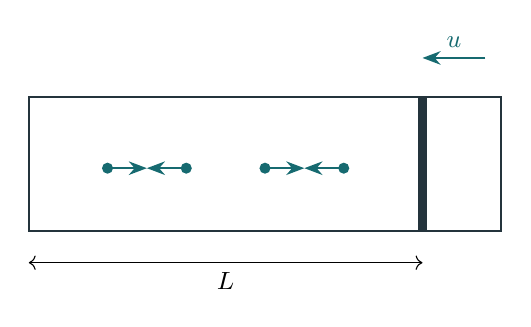
\begin{tikzpicture}[x=1cm,y=1cm,font=\small,every node/.append style={align=center}]\draw[object] (0,0) rectangle(6,1.7);\draw[object,line width=3pt] (5,0)--(5,1.7);\foreach \x/\d in {1/1,2/-1,3/1,4/-1}{\fill[accent] (\x,.8) circle(2pt);\draw[motion] (\x,.8)--(\x+.5*\d,.8);}\draw[motion] (5.8,2.2)--(5,2.2) node[midway,above]{$u$};\draw[<->] (0,-.4)--(5,-.4) node[midway,below]{$L$};\end{tikzpicture}\figcaption{图 热3.4　小球只作一维运动，右活塞缓慢内推。}\end{minipage}\end{center}

\Needspace{5\baselineskip}

\pdfbookmark[3]{题型定位}{q4-h0}

\subsection*{题型定位}

从移动壁上的反射与往返碰撞间隔导出一维绝热规律，再从端面压强和一维热容量得到同一指数。

\Needspace{5\baselineskip}

\pdfbookmark[3]{知识点}{q4-h1}

\subsection*{知识点}

等质量小球弹性正碰交换速度。右活塞速度为 $-u$，入射速度 $v$ 的球反射后为 $-v-2u$。慢推给往返时间约 $2L/v$，从而 $vL$ 保持。平均能量 $U=NkT/2$ 和状态方程 $pV=NkT$ 给 $C_V=R/2$、$\gamma=3$。


\Needspace{5\baselineskip}

\pdfbookmark[3]{物理图像}{q4-h2}

\subsection*{物理图像}

解图热3.4A中，右壁向左，撞壁的小球比入射快。容器变短后，同一速率标签回到壁面的间隔也缩短。解图热3.4B并列两个参考系，在活塞系只将相对速度反号，回实验室系再加活塞速度。两球正碰时，更换追踪的球即可延续原来的速度标签。

\Needspace{5\baselineskip}

\pdfbookmark[3]{解题入口}{q4-h3}

\subsection*{解题入口}

先对同一次碰壁作两次速度变换，求速率增加 $2u$。除以往返时间后，用 $\dot L=-u$ 把增速写成 $L\dd v+v\dd L=0$。对每个速度标签先平方再平均，由温度定义和固定截面积得到 $TV^2$。


\Needspace{5\baselineskip}

\pdfbookmark[3]{标准解法}{q4-h4}

\subsection*{标准解法}

取管长$L$，活塞内推速率$u>0$，故$\dot L=-u$。相同球的弹性正碰只交换速度，可以追踪某一速率的“携带者”。
\begin{center}\begin{minipage}{0.96\linewidth}\centering\begin{tikzpicture}[x=1cm,y=1cm,font=\small,every node/.append style={align=center}]\draw[object] (0,0) rectangle(6,1.7);\draw[object,line width=3pt] (5,0)--(5,1.7);\foreach \x/\d in {1/1,2/-1,3/1,4/-1}{\fill[accent] (\x,.8) circle(2pt);\draw[motion] (\x,.8)--(\x+.5*\d,.8);}\draw[motion] (5.8,2.2)--(5,2.2) node[midway,above]{$u$};\draw[<->] (0,-.4)--(5,-.4) node[midway,below]{$L$};\node[above] at (2.5,2.2){$v\to v+2u$，两次碰壁间隔$2L/v$};\end{tikzpicture}\figcaption{解图 热3.4A　追踪速率携带者；单次增速与碰撞频率共同决定平均增能。}\end{minipage}\end{center}
取解图热3.4A向右为正，右端活塞速度为$-u$，迎面入射小球速度为$+v$。
转到活塞参考系，入射速度为$v-(-u)=v+u$。弹性反射使相对速度反号，回到实验室系后
\[
v_{\rm out}=-(v+u)+(-u)=-v-2u.
\]
出射方向向左，速度分量为 $-v-2u$，速率从 $v$ 增至 $v+2u$。
单次碰撞增加的动能为
\[
\Delta\varepsilon=\frac m2[(v+2u)^2-v^2]=2muv+2mu^2\simeq2muv.
\]
最后一步保留$u/v$的一阶项。小球到左壁反射后再回到活塞，在$u\ll v$下往返时间约为$2L/v$；
这一周期中活塞的位移与$L$之比为$2u/v\ll1$，可把碰撞序列视为慢变过程。于是
\[\dot v\simeq\frac{2u}{2L/v}=\frac{uv}{L},\qquad L\dd v+v\dd L=0.\]
对单球动能$\varepsilon=mv^2/2$，乘以$mv$得
\[L\dd\varepsilon+2\varepsilon\dd L=0.\]
各速度携带者遵循同一缩放，平均后
\[L\dd\langle\varepsilon\rangle+2\langle\varepsilon\rangle\dd L=0.\]
以$\langle\varepsilon\rangle=kT/2$定义温度，且$V=SL$，所以
\[\frac{\dd T}{T}+2\frac{\dd V}{V}=0,
\quad\ln\frac{T}{T_0}+2\ln\frac{V}{V_0}=0.\]
\result{TV^2=T_0V_0^2.}
\textbf{一维气体的内能与绝热关系。} 一维只有一个平动自由度，$U=NkT/2$。端面压力由碰撞频率与冲量相乘，$p=Nm\langle v^2\rangle/V=NkT/V$。绝热时
\[\dd U=-p\dd V\ \Rightarrow\ \frac12Nk\dd T=-\frac{NkT}{V}\dd V,\]
分离变量积分得到上面的$TV^2=T_0V_0^2$。一维$C_V=R/2,C_p=C_V+R=3R/2$，故$\gamma=3$。慢压缩时，活塞速率远小于小球的典型速率，相邻两次碰撞之间的容器长度只改变一小段，因而可以用上面的连续微分式描述平均能量变化。
\subsubsection*{把单次反射、碰撞间隔与连续压缩连起来}
解图热3.4B分别在实验室系和活塞系标出速度，
向右为同一正方向。实验室系活塞速度是$-u$，
入射速度$+v$；活塞系入射为$+(v+u)$，反射后为$-(v+u)$。
加回活塞的$-u$，才得到实验室系的$-(v+2u)$。
所增的是速率$2u$，速度分量本身则从正变负。

\begin{center}\begin{minipage}{0.96\linewidth}\centering
\begin{tikzpicture}[x=1cm,y=1cm,font=\small]
\begin{scope}
\draw[object,line width=2pt] (3,0)--(3,2);
\draw[motion] (.3,1.4)--(2.4,1.4) node[midway,above] {$+v$};
\draw[motion] (2.4,.5)--(.3,.5) node[midway,below] {$-v-2u$};
\draw[motion] (3.4,2.3)--(2.6,2.3) node[midway,above] {$-u$};
\node[above] at (1.4,3) {实验室系};
\end{scope}
\begin{scope}[xshift=6cm]
\draw[object,line width=2pt] (3,0)--(3,2);
\draw[motion] (.3,1.4)--(2.4,1.4) node[midway,above] {$+(v+u)$};
\draw[motion] (2.4,.5)--(.3,.5) node[midway,below] {$-(v+u)$};
\node[above] at (3,2.3) {活塞静止};
\node[above] at (1.4,3) {活塞系};
\end{scope}
\end{tikzpicture}
\figcaption{解图 热3.4B　两参考系使用同一正方向；在活塞系作弹性反射，再变回实验室系。}
\end{minipage}\end{center}
单次增能$2muv+2mu^2$中的二次项与一次项之比为$u/v$。
往返时间$2L/v$内，活塞相对位移约$2uL/v$，
与 $L$ 之比为 $2u/v$。慢推使同一次往返的容器长度改变量和速率改变量都很小，分别控制碰撞间隔与增能的近似。

相同小球的弹性正碰只交换速度；
将速度标签跟随碰撞继续传递，等效于标签轨迹穿过彼此。
连续追踪这个速率时，球间每发生一次交换，就转到携带同一速率的另一球。
慢变极限给
\[
L\dd v+v\dd L=0,\qquad
\dd(Lv)=0,\qquad
v=v_0\frac{L_0}{L}.
\]
平方后逐个携带者都有
\[
\varepsilon L^2=\varepsilon_0L_0^2,\qquad
L\dd\varepsilon+2\varepsilon\dd L=0.
\]
容器长度L对所有标签相同，因此对这条关系平均可得到
$\langle\varepsilon\rangle L^2$恒定，
再由温度定义得到$TL^2$恒定。
截面积保持S不变，$V/V_0=L/L_0$，才转为$TV^2$恒定。

\subsubsection*{从端面冲量独立求压强和热容量}
在同一慢变、随机相位的近似下，
一个速率v的球撞固定端面的频率为$v/(2L)$，
每次法向冲量$2mv$，因此平均力为$mv^2/L$。
对N个球求和并除截面积S，
\[
p=\frac{Nm\langle v^2\rangle}{SL}
=\frac{2N\langle\varepsilon\rangle}{V}
=\frac{NkT}{V}.
\]
系统总能量$U=N\langle\varepsilon\rangle=NkT/2$，
绝热内推的外界功使$\dd U=-p\dd V$，故
\[
V\dd T+2T\dd V=0,\qquad
\ln(T/T_0)+2\ln(V/V_0)=0.
\]
由$pV=NkT$还可得
\[
pV^3=p_0V_0^3,\qquad
T/T_0=(V_0/V)^2,\qquad p/p_0=(V_0/V)^3.
\]
体积减半时，上式给温度为4倍、压强为8倍。

一般能量均分模型中，设有效二次项数$i=t+r+2s$，
t为平动项数，r为转动项数，s个已激发振动模式各含动能与势能两项。
有
\[
C_V=\frac i2R,\qquad C_p=\frac{i+2}{2}R,\qquad
\gamma=\frac{i+2}{i}.
\]
本题为只作一维平动的质点，$t=1,r=s=0$，
所以$i=1,\gamma=3$，代$TV^{\gamma-1}$仍给$TV^2$。
三维单原子气体有三个平动项，$t=3$，由同一热容量关系得到 $\gamma=5/3$。

温度由平均动能定义。相同质点的一维弹性碰撞交换已有的速度，保留速率分布。慢推时，各速度标签按同一因子缩放，因而任一给定初始分布都可用该缩放关系求平均能量。$u/v\ll1$ 适用于贡献主要动能的典型速率。若活塞速度可与球速相比，改用实际的相遇时刻和反射速度逐次计算。


\Needspace{5\baselineskip}

\pdfbookmark[3]{关键洞察}{q4-h5}

\subsection*{关键洞察}

慢推时各速率标签按共同因子放大，温度从平均动能取得。相同质点的一维碰撞只交换已有的速度。压强来自每次冲量与频率的乘积，平均对象为 $v^2$。

\Needspace{5\baselineskip}

\pdfbookmark[3]{易错点}{q4-h6}

\subsection*{易错点}

\begin{itemize}
\item 出射速度分量为负，速率取其绝对值。回到实验室系时加上活塞的速度 $-u$。
\item 单次速度改变量除回到同一端面的往返时间，才得到连续变化率。
\item 先求各小球的 $v^2$ 再平均；一个平动自由度给 $\langle\varepsilon\rangle=kT/2$。
\item 截面积固定时 $V/V_0=L/L_0$。有限壁速下可从实际碰壁时刻求长度与速度。
\end{itemize}

\Needspace{5\baselineskip}

\pdfbookmark[3]{课堂讲解建议}{q4-h7}

\subsection*{课堂讲解建议}

在解图热3.4B上沿着入射、反射、变回三个步骤写速度。让两位学生分别追踪球的编号和碰撞时传递的速度标签，说出两种轨迹的区别。再用解图热3.4A把每次增速与往返时间联系起来。

用变图热3.4V4从端面冲量求压强，代第一定律得到温度指数。最后读变图热3.4V5体积减半处的温度和压强，追问两个指数为何相差一。

\Needspace{5\baselineskip}

\pdfbookmark[3]{变式训练}{q4-h8}

\subsection*{变式训练}

\begin{enumerate}
\item 改为平面内运动，气体能在两个方向之间较快交换能量。变图热3.4V1的活塞沿 $x$ 推动，面积 $A$ 改变。共同温度下 $\langle mv_x^2\rangle=kT$，故二维压力满足 $pA=NkT$。气体有两个平动二次项，总内能为 $NkT$，绝热时
\[
Nk\dd T=-p\dd A=-NkT\frac{\dd A}{A}.
\]
因此 $TA$ 恒定。若两分量各自演化且没有能量交换，沿压缩方向的能量按一维规律计算，另一方向的能量保持。
\begin{center}\begin{minipage}{.98\linewidth}\centering
\begin{tikzpicture}[scale=.85,transform shape]
\draw[object](0,0)rectangle(5.4,2.56);
\draw[object,line width=2.2pt](4.28,0)--(4.28,2.56);
\draw[motion](5.1,2.96)--(4.28,2.96)node[midway,above]{$u$};
\coordinate (B)at(2.45,1.12);
\fill[accent](B)circle(2pt);
\draw[motion](B)--(3.5,1.12)node[below]{$v_x$};
\draw[motion](B)--(2.45,2.08)node[above]{$v_y$};
\draw[guide](2.45,2.08)--(3.5,2.08)--(3.5,1.12);
\node at(1.2,.45){面积 $A$};
\draw[<->](0,-.45)--(4.28,-.45)node[midway,below]{$L$};
\end{tikzpicture}
\figcaption{变图热3.4V1\quad 二维气体经足够快的能量交换，共享同一温度}
\end{minipage}\end{center}
\item 给定压缩比 $q=V_i/V_f$。对 $i$ 个可充分交换能量的平动二次项，$C_V=iR/2$，故 $T_f/T_i=q^{2/i}$。变图热3.4V2的实线 $q^2$ 用 $i=1$，虚线 $q^{2/3}$ 用 $i=3$，对应 $\gamma=3$ 和 $5/3$。例如 $q=2$ 时，两图线的读数分别为4和 $2^{2/3}$。
\begin{center}\begin{minipage}{.98\linewidth}\centering
\begin{tikzpicture}[scale=.85,transform shape]
\begin{scope}[x=2.36cm,y=.59cm]
\draw[axis](.66,0)--(2.57,0)node[right]{$q=V_i/V_f$};
\draw[axis](.66,0)--(.66,6.6)node[above]{$T_f/T_i$};
\draw[traj,domain=1:2.36,samples=75]plot(\x,{\x^2})node[above left]{一维};
\draw[object,dashed,domain=1:2.36,samples=75]plot(\x,{pow(\x,2/3)})node[above right]{三维};
\draw[guide](2,0)--(2,4);
\fill[accent](2,4)circle(1.5pt)node[above left]{$4$};
\fill(2,{pow(2,2/3)})circle(1.5pt)node[below left]{$2^{2/3}$};
\node[below]at(2,0){$2$};
\end{scope}
\end{tikzpicture}
\figcaption{变图热3.4V2\quad 给相同压缩比时，一个平动方向的升温大于三个方向的升温}
\end{minipage}\end{center}
\item 若活塞以恒定速率 $u$ 快速内推，一次反射后球速大小仍为 $v'=v+2u$。设刚反射时管长为 $L_0$，取此时 $t=0$。变图热3.4V3中球先用 $t_{\text{左}}=L_0/v'$ 到左端，再满足 $v'(t-t_{\text{左}})=L_0-ut$ 时遇到活塞，故 \(t_1=2L_0/(v'+u)\)，$L_1=L_0-ut_1$。图取 $L_0=4,v=2,u=1/2$ 的示意尺度。每个速度标签由自己的折线交点决定相遇时刻，整团气体的某一时刻平均动能应逐标签求和。
\begin{center}\begin{minipage}{.98\linewidth}\centering
\begin{tikzpicture}[scale=.85,transform shape]
\begin{scope}[x=2cm,y=.72cm]
\draw[axis](0,0)--(2.95,0)node[right]{$t$};
\draw[axis](0,0)--(0,4.55)node[above]{$x$};
\draw[object](0,4)--(2.6,2.7)node[right]{活塞};
\draw[motion](0,4)--({4/3},0);
\draw[motion]({4/3},0)--({16/7},{20/7});
\fill[accent](0,4)circle(1.6pt)node[left]{$L_0$};
\fill[accent]({16/7},{20/7})circle(1.6pt)node[above right]{$L_1$};
\draw[guide]({16/7},0)--({16/7},{20/7});
\node[below]at({4/3},0){$t_{\text{左}}$};
\node[below]at({16/7},0){$t_1$};
\node at(1.7,3.54){斜率 $-u$};
\end{scope}
\end{tikzpicture}
\figcaption{变图热3.4V3\quad 有限推进速率下，按球的折线与活塞位置线的交点确定下次碰撞}
\end{minipage}\end{center}
\item 变图热3.4V4追踪速率为 $v$ 的球。缓慢移动条件下以瞬时 $L$ 估算，每 $2L/v$ 撞同一端面一次，一次给端面法向冲量 $2mv$，故平均力为 $mv^2/L$。对不同球求和，
\[
p=\frac{m\sum_{j=1}^Nv_j^2}{SL}=\frac{Nm\langle v^2\rangle}{V}=\frac{NkT}{V}.
\]
往返频率和冲量各含一次 $v$，所以平均的是各球的速率平方。
\begin{center}\begin{minipage}{.98\linewidth}\centering
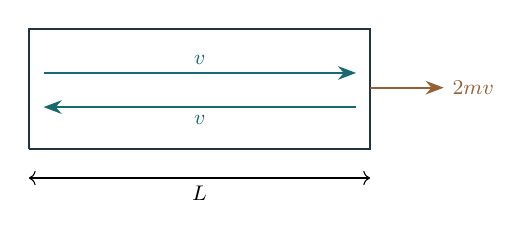
\begin{tikzpicture}[scale=.85,transform shape]
\draw[object](0,0)--(0,1.8)--(5.1,1.8)--(5.1,0)--(0,0);
\draw[motion](.22,1.14)--(4.89,1.14)node[midway,above]{$v$};
\draw[motion](4.89,.63)--(.22,.63)node[midway,below]{$v$};
\draw[force](5.1,.92)--(6.2,.92)node[right]{$2mv$};
\draw[<->](0,-.43)--(5.1,-.43)node[midway,below]{$L$};
\end{tikzpicture}
\figcaption{变图热3.4V4\quad 每完成一次往返，球向同一个端面传递一次大小为 $2mv$ 的冲量}
\end{minipage}\end{center}
\item 令 $V_f=V_0/2$。变图热3.4V5中温度满足 $(V_0/V)^2$，减半处读4。由 $pV=NkT$ 知压强还多一个 $V_0/V$ 的因子，同一竖线上读8。因此 $p_fV_f^3=8p_0(V_0/2)^3=p_0V_0^3$。
\begin{center}\begin{minipage}{.98\linewidth}\centering
\begin{tikzpicture}[scale=.85,transform shape]
\begin{scope}[x=4.8cm,y=.415cm]
\draw[axis](.35,0)--(1.13,0)node[right]{$V/V_0$};
\draw[axis](.35,0)--(.35,9.35)node[above]{归一化值};
\draw[traj,domain=.5:1.06,samples=74]plot(\x,{1/\x^2});
\draw[object,dashed,domain=.5:1.06,samples=74]plot(\x,{1/\x^3});
\draw[guide](.5,0)--(.5,8);
\draw[guide](.35,4)--(.5,4);
\draw[guide](.35,8)--(.5,8);
\fill[accent](.5,4)circle(1.5pt)node[above right]{$T/T_0$};
\fill(.5,8)circle(1.5pt)node[above right]{$p/p_0$};
\fill(1,1)circle(1.5pt);
\node[below]at(.5,0){$1/2$};\node[below]at(1,0){$1$};
\node[left]at(.35,4){$4$};\node[left]at(.35,8){$8$};
\end{scope}
\end{tikzpicture}
\figcaption{变图热3.4V5\quad 体积从 $V_0$ 减半到 $V_0/2$，温度增为四倍，压强增为八倍}
\end{minipage}\end{center}
\item 在一次往返内把 $L,v$ 看成固定量。变图热3.4V6的上边为从左至右的 $p_x=mv$，下边为从右至左的 $p_x=-mv$。两条竖边碰壁时 $\dd x=0$，所以
\[
\oint p_x\dd x=mvL+(-mv)(-L)=2mvL .
\]
慢变关系 $\dd(vL)=0$ 便使此作用量近似恒定。若壁速较大，各段用实际碰撞时的 $L$ 与反射动量。
\begin{center}\begin{minipage}{.98\linewidth}\centering
\begin{tikzpicture}[scale=.85,transform shape]
\fill[accent!16](0,-.98)rectangle(4.53,.98);
\draw[axis](-.57,0)--(5.73,0)node[right]{$x$};
\draw[axis](0,-1.53)--(0,1.61)node[above]{$p_x$};
\draw[traj](0,.98)--(4.53,.98)--(4.53,-.98)--(0,-.98)--cycle;
\draw[motion](1.1,.98)--(3.2,.98);
\draw[motion](3.3,-.98)--(1.2,-.98);
\node[left]at(0,.98){$mv$};
\node[left]at(0,-.98){$-mv$};
\node[below right]at(4.53,0){$L$};
\node at(2.27,.39){面积 $2mvL$};
\end{tikzpicture}
\figcaption{变图热3.4V6\quad 固定瞬时参数时，一个往返在相平面围出矩形}
\end{minipage}\end{center}
\item 给小球增加一个可以与平动迅速交换能量的内部二次项，且轴向压强仍由平动传递。变图热3.4V7的两项各有平均能量 $kT/2$，故 $U=NkT$、$C_V=R$。用 $pV=NkT$ 得 $\gamma=1+R/C_V=2$，以及 $TV$ 恒定。可取与小球平动耦合的一个转动二次项作为例子，交换时间短于压缩时间时才有图中的共同温度。
\begin{center}\begin{minipage}{.98\linewidth}\centering
\begin{tikzpicture}[scale=.85,transform shape]
\draw[axis](0,0)--(6.1,0)node[right]{能量项};
\fill[accent!20](.95,.42)rectangle(2.32,2.63);
\fill[warm!20](3.67,.42)rectangle(5.04,2.63);
\node at(1.64,1.51){$kT/2$};
\node at(4.36,1.51){$kT/2$};
\node[above]at(1.64,2.68){轴向平动};
\node[above]at(4.36,2.68){额外二次项};
\draw[motion,<->](2.4,1.51)--(3.59,1.51);
\node[below]at(3,1.45){交换};
\end{tikzpicture}
\figcaption{变图热3.4V7\quad 额外的二次能量项和轴向平动充分交换能量时，各得一份 $kT/2$}
\end{minipage}\end{center}
\item 缓慢外移活塞，$\dot L=u>0$。变图热3.4V8的活塞系入射速度为 $v-u$，反射后回实验室系得 $-v+2u$。对 $v\gg u$ 的主要速率标签，速率减 $2u$，以 $2L/v$ 为往返间隔给 $\dot v\simeq-uv/L$。这与 $\dot L=u$ 合并仍给 $Lv$ 保持，所以 $TV^2$ 保持，气体膨胀降温。$v\leq u$ 时该球追不上向外移动的活塞。
\begin{center}\begin{minipage}{.98\linewidth}\centering
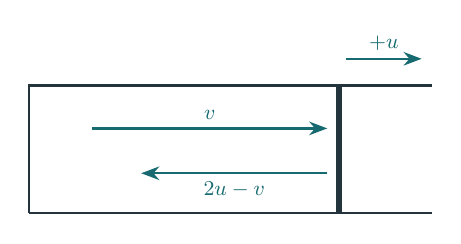
\begin{tikzpicture}[scale=.85,transform shape]
\draw[object](0,0)--(0,1.9)--(6.02,1.9);
\draw[object](0,0)--(6.02,0);
\draw[object,line width=2.2pt](4.63,0)--(4.63,1.9);
\draw[motion](4.74,2.3)--(5.87,2.3)node[midway,above]{$+u$};
\draw[motion](.95,1.26)--(4.46,1.26)node[midway,above]{$v$};
\draw[motion](4.46,.59)--(1.68,.59)node[midway,below]{$2u-v$};
\end{tikzpicture}
\figcaption{变图热3.4V8\quad 外移活塞与入射球同向，反射后球的速率减少}
\end{minipage}\end{center}
\end{enumerate}

\clearpage

\pdfbookmark[2]{第 5 题 光子气压强、能量密度与绝热方程}{q5}

\section*{第 5 题\quad 光子气压强、能量密度与绝热方程}

空腔中已经建立热平衡的热辐射可作为光子气处理，壁面对光子的反射用于计算动量通量。设辐射能量密度为$u$，求压强$p$；论证宏观热平衡辐射的$u$只由温度$T$决定；证明$p\propto T^4$，并导出准静态绝热过程的$p-V$关系。这里讨论热平衡辐射，光子数无独立守恒约束。

\begin{center}\begin{minipage}{0.96\linewidth}\centering\begin{tikzpicture}[x=1cm,y=1cm,font=\small]
\draw[object] (0,0) rectangle (5,4.2);
\node at (1.7,2.6) {热平衡辐射：$u,T$};
\draw[motion] (2,.2)--(5,2) node[pos=.28,below right] {入射};
\draw[motion] (5,2)--(2,3.8) node[pos=.35,above right] {反射};
\draw[guide] (3.5,2)--(5,2);
\draw (4.3,2) arc[start angle=180,end angle=149.036,radius=.7];
\node at (4.05,2.22) {$\theta$};
\draw[force] (5,2)--(6.2,2);
\node[above,align=center] at (6.15,2.45) {壁所受冲量\\$2\epsilon\cos\theta/c$};
\node[below right] at (5.03,1.94) {R};
\end{tikzpicture}\figcaption{图 热3.5　光子在壁面反射，法向动量发生改变。}\end{minipage}\end{center}

\Needspace{5\baselineskip}

\pdfbookmark[3]{题型定位}{q5-h0}

\subsection*{题型定位}

用光子反射和小孔交换确定 $p=u/3$ 与 $u=u(T)$，再由平衡态热力学导出温度四次方律和可逆绝热线。

\Needspace{5\baselineskip}

\pdfbookmark[3]{知识点}{q5-h1}

\subsection*{知识点}

单光子动量为 $\epsilon/c$。反射动量通量含两个方向余弦，单向小孔能流仅含一个。由 $F=U-TS$ 的两个一阶偏导得到 $(\partial U/\partial V)_T=T(\partial p/\partial T)_V-p$。光子数自由调整时，平衡态满足 $U=a_rVT^4$、$S=4a_rVT^3/3$。


\Needspace{5\baselineskip}

\pdfbookmark[3]{物理图像}{q5-h2}

\subsection*{物理图像}

解图热3.5A的 $R$ 点在反射壁上。以法线为参照，入射和反射光的切向动量相同，壁面接收两倍入射法向动量。解图热3.5B的两支交换箭头都穿过同一个孔，两腔同温且热平衡时两箭头表示等大的单向能流。

\Needspace{5\baselineskip}

\pdfbookmark[3]{解题入口}{q5-h3}

\subsection*{解题入口}

单光子的法向冲量乘到达数，并在入射半球积分。对小孔改求穿过的能量，比较同温两腔的能流。用 $U=uV$ 和 $p=u/3$ 代入自由能偏导得到微分方程。可逆绝热时把 $\dd U=-p\dd V$ 写成关于 $p,V$ 的方程。


\Needspace{5\baselineskip}

\pdfbookmark[3]{标准解法}{q5-h4}

\subsection*{标准解法}

\textbf{辐射压。} 光子能量$\epsilon=h\nu$、动量大小$\epsilon/c$。取壁面法向$x$，入射方向余弦$\cos\theta>0$；反射传递$2(\epsilon/c)\cos\theta$。各向同性时方向的能量密度为$u\dd\Omega/(4\pi)$，入射能流再乘$c\cos\theta$。故
\[p=\frac{2u}{4\pi}\int_{\rm hemisphere}\cos^2\theta\dd\Omega
=\frac{u}{2\pi}\,2\pi\int_0^{\pi/2}\cos^2\theta\sin\theta\dd\theta=\frac u3.\]
\begin{center}\begin{minipage}{0.96\linewidth}\centering\begin{tikzpicture}[x=1cm,y=1cm,font=\small]
\draw[object] (0,0) rectangle (5,4.2);
\node at (1.7,2.6) {热平衡辐射：$u,T$};
\draw[motion] (2,.2)--(5,2) node[pos=.28,below right] {入射};
\draw[motion] (5,2)--(2,3.8) node[pos=.35,above right] {反射};
\draw[guide] (3.5,2)--(5,2);
\draw (4.3,2) arc[start angle=180,end angle=149.036,radius=.7];
\node at (4.05,2.22) {$\theta$};
\draw[force] (5,2)--(6.2,2);
\node[above,align=center] at (6.15,2.45) {壁所受冲量\\$2\epsilon\cos\theta/c$};
\node[below right] at (5.03,1.94) {R};
\end{tikzpicture}\figcaption{解图 热3.5A　入射能流与反射冲量分别带一个方向余弦，角积分给$1/3$。}\end{minipage}\end{center}
解图热3.5A的反射几何中，一个$\cos\theta$来自每次碰壁的法向动量变化，另一个来自单位时间能撞到壁面的入射能流；两者相乘才得到压强积分中的$\cos^2\theta$。解图热3.5B则比较同温两腔穿过小孔的双向通量，两腔各自已热化，同温使两向能流相等，从而确定共同的 $u(T)$。

各频率的压强贡献为$p_\nu=u_\nu/3$，再求和得到总压强；光子的动量关系不需要静止质量。

\textbf{能量密度与温度。} 让两个同温的宏观空腔经很小的孔交换热平衡辐射。按解图热3.5B的箭头，两边射入对侧的能量通量分别是 $cu_1/4$ 和 $cu_2/4$。热平衡时它们相等，故 $u_1=u_2$；在这个各向同性的空腔模型中，平衡能量密度只由共同温度确定，记作 $u(T)$。
\begin{center}\begin{minipage}{0.96\linewidth}\centering\begin{tikzpicture}[x=1cm,y=1cm,font=\small]
\draw[object,fill=accent!5] (0,0) rectangle (6,2.5);
\draw[object] (3,0)--(3,1.05) (3,1.45)--(3,2.5);
\node[align=center] at (1.15,1.25) {空腔A\\$T,u_A$};
\node[align=center] at (4.85,1.25) {空腔B\\$T,u_B$};
\draw[motion] (2.1,1.35)--(3.9,1.35);
\draw[force] (3.9,1.15)--(2.1,1.15);
\node[text=accent] at (1.5,2.05) {$cu_A/4$};
\node[text=warm] at (4.5,.4) {$cu_B/4$};
\node[above] at (3,2.75) {同温辐射交换};
\end{tikzpicture}\figcaption{解图 热3.5B　热平衡要求穿孔的两向能量通量相等，宏观辐射能量密度一致。}\end{minipage}\end{center}
同温论证用的是已热化的两腔。若用带活塞的循环表述这一论证，循环末应恢复两腔及活塞状态。理想镜壁只改变光线方向，镜面腔内的未热化光束可以保留由初态决定的能量密度。

\textbf{求温度律。} $U=u(T)V$，可逆微分$\dd U=T\dd S-p\dd V$。令$F=U-TS$，则$\dd F=-S\dd T-p\dd V$，混合偏导相等给
\[\left(\frac{\partial S}{\partial V}\right)_T=\left(\frac{\partial p}{\partial T}\right)_V,\quad
\left(\frac{\partial U}{\partial V}\right)_T=T\left(\frac{\partial p}{\partial T}\right)_V-p.\]
代入$p=u/3$与$U=uV$：
\[u=\frac T3\frac{\dd u}{\dd T}-\frac u3,
\quad\frac{\dd u}{u}=4\frac{\dd T}{T}.
\]
因此 $u=a_rT^4$，$p=a_rT^4/3$。比例常数 $a_r$ 由辐射的微观统计确定，或由一个参考态的 $u/T^4$ 得到。

\textbf{准静态绝热。} $\dd U=-p\dd V$，而$U=3pV$，
\[3V\dd p+3p\dd V=-p\dd V,
\quad\frac{\dd p}{p}=-\frac43\frac{\dd V}{V}.\]
\result{pV^{4/3}=\text{常量},\qquad TV^{1/3}=\text{常量}.}
同一曲线也由 $S=4a_rVT^3/3$ 恒定给出。$4/3$ 是绝热压强曲线的指数。热平衡光子气的压强由温度确定，定压过程也等温，通常用升温定义的 $C_p$ 在这里没有独立定义。
\subsubsection*{把半球通量、频率分量与总能量密度分清}
解图热3.5A的入射点就在反射壁上，反射前后切向动量相同，
法向动量反号。以指向壁外为正，壁所受冲量为正，
而光子所受法向冲量为负，两者大小相等。
频率落在一个小区间内的光子，能量密度记为$u_\nu\dd\nu$；
单光子能量为$h\nu$，动量大小为$h\nu/c$，
故同一角积分给
\[
p_\nu\dd\nu=\frac13u_\nu\dd\nu,\qquad
p=\int_0^\infty p_\nu\dd\nu
=\frac13\int_0^\infty u_\nu\dd\nu=\frac u3.
\]
反射计算直接用光子动量 $h\nu/c$。这里的 $u$ 合计腔内所有传播方向和频率。讨论定向光束时，可分别记入射能量密度、反射能量密度和两者之和。

解图热3.5B中两支箭头都穿过隔板的小孔。
一次穿孔的能量没有反射冲量因子，其单位面积单向能流为
\[
J_E=\frac{cu}{4\pi}\int_{\rm hemisphere}\cos\theta\dd\Omega
=\frac{cu}{4\pi}\,2\pi\int_0^{\pi/2}\cos\theta\sin\theta\dd\theta
=\frac{cu}{4}.
\]
因此同温两腔的净能流密度为$c(u_A-u_B)/4$。
本题已给出热平衡辐射，且光子数没有独立守恒约束；
宏观热平衡的同温两腔，穿孔净交换为零，所以两腔的能量密度相同。壁与辐射交换能量并参与热化时，腔内能量密度可由平衡温度确定。

\subsubsection*{从自由能逐项推出温度四次方律}
在平衡状态空间以T、V为独立变量，写
\[
S=-\left(\frac{\partial F}{\partial T}\right)_V,\qquad
p=-\left(\frac{\partial F}{\partial V}\right)_T.
\]
对第一式求V偏导，对第二式求T偏导，
利用F的混合偏导交换，便得到前面的麦克斯韦关系。
另一方面，在$\dd T=0$时由$\dd U=T\dd S-p\dd V$得
\[
\left(\frac{\partial U}{\partial V}\right)_T
=T\left(\frac{\partial S}{\partial V}\right)_T-p
=T\left(\frac{\partial p}{\partial T}\right)_V-p.
\]
等温偏导比较的是温度相同而体积略有不同的相邻平衡态。
左边对$U=u(T)V$求导为u，右边的压强导数为$u'(T)/3$，
所以$3u=Tu'-u$，即$Tu'=4u$。取一个非零温度参考态，
\[
\ln\frac{u}{u_0}=4\ln\frac{T}{T_0},\qquad
\frac{u}{u_0}=\left(\frac{T}{T_0}\right)^4,\qquad
\frac{p}{p_0}=\left(\frac{T}{T_0}\right)^4.
\]
常数$a_r=u_0/T_0^4$的单位为$\mathrm{J\,m^{-3}\,K^{-4}}$。
其具体数值需要辐射的微观统计，现有热力学关系只确定幂次。

\subsubsection*{光子气的熵、绝热线和等温供热}
代$U=a_rVT^4$和$p=a_rT^4/3$，有
\[
\dd U=4a_rVT^3\dd T+a_rT^4\dd V,
\qquad
\dd S=\frac{\dd U+p\dd V}{T}
=4a_rVT^2\dd T+\frac43a_rT^3\dd V.
\]
右边正是$\dd(4a_rVT^3/3)$，故
\[
S=\frac43a_rVT^3+S_0.
\]
在零温辐射熵取零的宏观模型中，$S_0=0$。
可逆绝热保持S不变，遂有$VT^3$不变，
从而$TV^{1/3}$、$pV^{4/3}$都不变；
总能量$U=a_rVT^4$则满足$UV^{1/3}$不变。
体积增加时温度降低，内能减少量转为壁面对外作功，符号与$\dd U=-p\dd V$一致。
若改为等温膨胀，辐射能量密度不变但总能量随体积增加：
\[
\Delta U=u\Delta V,\qquad W=\frac u3\Delta V,\qquad
Q=\Delta U+W=\frac43u\Delta V.
\]
定容时总热容量为$4a_rVT^3$。
光子气的压强由温度唯一决定，定压过程同时是等温过程。此时供热可以随体积变化，温升恒为零。通常以非零温升定义的定压热容量在这里没有定义，绝热指数$4/3$由熵随$V,T$的变化确定。


\Needspace{5\baselineskip}

\pdfbookmark[3]{关键洞察}{q5-h5}

\subsection*{关键洞察}

法向冲量和到达速率各给一个方向余弦，穿孔只保留到达因子。宏观平衡辐射由 $T$ 定能量密度，热力学关系确定其幂次。$a_r$ 的数值由平衡辐射的微观光谱确定。同样计算定向束流时，要指明能量密度包括哪几个传播方向。

\Needspace{5\baselineskip}

\pdfbookmark[3]{易错点}{q5-h6}

\subsection*{易错点}

\begin{itemize}
\item 单光子直接用动量大小 $\epsilon/c$，壁面反射后能量不变，法向动量分量反号。
\item 小孔交换按每个方向的能量通量求和。两同温平衡腔各自都有单向通量 $cu/4$。
\item 求温度律时用等温偏导。求绝热线时才用可逆绝热的 $\dd U=-p\dd V$。
\item 等温膨胀的供热同时支付新增辐射能量和壁面功。
\end{itemize}

\Needspace{5\baselineskip}

\pdfbookmark[3]{课堂讲解建议}{q5-h7}

\subsection*{课堂讲解建议}

在解图热3.5A的 $R$ 点把动量拆成法向和切向分量，让学生先算壁面收到的冲量，再给到达数乘余弦。接着用解图热3.5B问小孔为什么只出现一个余弦。

由自由能的两个一阶偏导指明取偏导时各固定哪个变量，再代入 $u$ 和 $p=u/3$。把变图热3.5V3与V6放在一起比较，说明同样膨胀时，绝热过程的壁面功由内能减少提供，等温过程的内能反而随体积增加。

\Needspace{5\baselineskip}

\pdfbookmark[3]{变式训练}{q5-h8}

\subsection*{变式训练}

\begin{enumerate}
\item 定容时以 $U=a_rVT^4$ 对温度求导，
\[
C_V=\left(\frac{\partial U}{\partial T}\right)_V=4a_rVT^3 .
\]
变图热3.5V1以参考态的 $T_0,U_0$ 无量纲化，切线斜率为4，因此在该状态 $C_V=4U_0/T_0$。总热容量单位为 $\mathrm{J/K}$。除以腔体体积得每单位体积的 $4a_rT^3$，单位为 $\mathrm{J/(m^3 K)}$。
\begin{center}\begin{minipage}{.98\linewidth}\centering
\begin{tikzpicture}[scale=.85,transform shape]
\begin{scope}[x=2.18cm,y=2.13cm]
\draw[axis](0,0)--(2.55,0)node[right]{$T/T_0$};
\draw[axis](0,0)--(0,1.64)node[above]{$U/U_0$};
\draw[traj,domain=.2:1.098,samples=85]plot(\x,{\x^4});
\draw[object,dashed,domain=.76:1.135,samples=25]plot(\x,{1+4*(\x-1)});
\fill[accent](1,1)circle(1.5pt)node[above left]{$(1,1)$};
\node[right]at(1.2,1.43){定容切线};
\node[right]at(1.2,.93){$C_VT_0/U_0=4$};
\end{scope}
\end{tikzpicture}
\figcaption{变图热3.5V1\quad 给定腔体体积，能量曲线的切线给总定容热容量}
\end{minipage}\end{center}
\item 将内能写为 $U=apV$。由 $\dd U=-p\dd V$ 得 $aV\dd p=-(a+1)p\dd V$。积分给 $pV^{1+1/a}$ 恒定。辐射的 $a=3$，三维单原子气体的 $a=3/2$，变图热3.5V2两曲线依次为 $(V/V_0)^{-4/3}$、$(V/V_0)^{-5/3}$。光子气的 $p$ 唯一确定温度，定压过程的温升为零，故其 $4/3$ 由绝热方程定义。
\begin{center}\begin{minipage}{.98\linewidth}\centering
\begin{tikzpicture}[scale=.85,transform shape]
\begin{scope}[x=2.15cm,y=2.15cm]
\draw[axis](.57,0)--(2.63,0)node[right]{$V/V_0$};
\draw[axis](.57,0)--(.57,1.78)node[above]{$p/p_0$};
\draw[traj,domain=1:2.45,samples=75]plot(\x,{pow(\x,-4/3)});
\draw[object,dashed,domain=1:2.45,samples=75]plot(\x,{pow(\x,-5/3)});
\fill[accent](1,1)circle(1.5pt)node[above right]{$(1,1)$};
\node[right]at(2.45,{pow(2.45,-4/3)}){辐射};
\node[below right]at(2.45,{pow(2.45,-5/3)}){三维单原子};
\end{scope}
\end{tikzpicture}
\figcaption{变图热3.5V2\quad 从同一归一化起点膨胀，三维单原子气体的压强下降更快}
\end{minipage}\end{center}
\item 可逆绝热地使 $V_f=2V_i$。由 $TV^{1/3}$ 恒定得 $T_f/T_i=2^{-1/3}$，四次方律给 $p_f/p_i=2^{-4/3}$。再用 $U=3pV$，得到 $U_f/U_i=2^{-1/3}$，如变图热3.5V3所示。压强与能量密度同倍率变化，总能量另乘终态体积比2。辐射减少的总能量等于对外所做的功 $U_i(1-2^{-1/3})$。
\begin{center}\begin{minipage}{.98\linewidth}\centering
\begin{tikzpicture}[scale=.85,transform shape]
\begin{scope}[x=3.6cm,y=2.8cm]
\draw[axis](.6,0)--(2.23,0)node[right]{$V/V_i$};
\draw[axis](.6,0)--(.6,1.23)node[above]{终态/初态};
\draw[traj,domain=1:2.08,samples=75]plot(\x,{pow(\x,-1/3)});
\draw[object,dashed,domain=1:2.08,samples=75]plot(\x,{pow(\x,-4/3)});
\draw[guide](2,0)--(2,{pow(2,-1/3)});
\fill[accent](2,{pow(2,-1/3)})circle(1.5pt)node[left]{$T/T_i=U/U_i$};
\fill(2,{pow(2,-4/3)})circle(1.5pt)node[above right]{$p/p_i$};
\node[below]at(2,0){$2$};
\end{scope}
\end{tikzpicture}
\figcaption{变图热3.5V3\quad 绝热加倍体积时，温度与总能量比相同，压强比另外包含体积因子}
\end{minipage}\end{center}
\item 固定光子数。若腔壁只反射，光谱仍取决于初态与腔内的热化机制。若有守恒光子数的相互作用可建立受限的热平衡，可用光子化学势 $\mu_\gamma$ 表示额外的数目约束：
\[
\bar n_\nu=\left[\exp((h\nu-\mu_\gamma)/(kT))-1\right]^{-1}.
\]
变图热3.5V4比较同温度下 $\mu_\gamma=0$ 与一个 $\mu_\gamma<0$ 的例子。热辐射能通过吸收和发射自由调整光子数时取 $\mu_\gamma=0$，得到本题的四次方律。反射时的能量与动量关系仍可用于求受限辐射的壁面动量通量。
\begin{center}\begin{minipage}{.98\linewidth}\centering
\begin{tikzpicture}[scale=.85,transform shape]
\begin{scope}[x=1.35cm,y=1.6cm]
\draw[axis](0,0)--(4.61,0)node[right]{$h\nu/(kT)$};
\draw[axis](0,0)--(0,2.32)node[above]{$\bar n_\nu$};
\draw[traj,domain=.395:4.28,samples=85]plot(\x,{1/(exp(\x)-1)});
\draw[object,dashed,domain=.395:4.28,samples=85]plot(\x,{1/(2.5*exp(\x)-1)});
\node[above right]at(.68,1.18){$\mu_\gamma=0$};
\node[above right]at(1.02,.29){$\exp(\mu_\gamma/kT)=0.4$};
\end{scope}
\end{tikzpicture}
\figcaption{变图热3.5V4\quad 同一温度下，光子数的约束可改变平衡占据数}
\end{minipage}\end{center}
\item 从 $U=a_rVT^4$ 与 $p=a_rT^4/3$ 出发，
\[
\dd S=\frac{\dd U+p\dd V}{T}
=4a_rVT^2\dd T+\frac43a_rT^3\dd V
=\dd\left(\frac43a_rVT^3\right).
\]
取零温熵为零，积分得到 $S=4a_rVT^3/3$。变图热3.5V5中两条等熵线的 $VT^3$ 分别为 $V_0T_0^3$ 与 $1.5V_0T_0^3$。沿任一条线有 $T\propto V^{-1/3}$，再由 $p\propto T^4$ 得 $p\propto V^{-4/3}$。
\begin{center}\begin{minipage}{.98\linewidth}\centering
\begin{tikzpicture}[scale=.85,transform shape]
\begin{scope}[x=2.15cm,y=2.32cm]
\draw[axis](.68,.45)--(3.3,.45)node[right]{$V/V_0$};
\draw[axis](.68,.45)--(.68,1.38)node[above]{$T/T_0$};
\draw[traj,domain=.82:3.12,samples=75]plot(\x,{pow(\x,-1/3)});
\draw[object,dashed,domain=.82:3.12,samples=75]plot(\x,{pow(1.5/\x,1/3)});
\fill[accent](1,1)circle(1.5pt)node[below left]{$(1,1)$};
\node[below right]at(3.07,{pow(3.07,-1/3)}){$S_*$};
\node[above right]at(3.07,{pow(1.5/3.07,1/3)}){$1.5S_*$};
\end{scope}
\end{tikzpicture}
\figcaption{变图热3.5V5\quad 在温度与体积图上，等熵线以 $VT^3$ 的值区分}
\end{minipage}\end{center}
\item 可逆等温膨胀 $\Delta V$ 时，$u,p$ 保持。变图热3.5V6柱子的下段为新增辐射能 $\Delta U=u\Delta V$，上段为 $W=\int p\dd V=u\Delta V/3$。第一定律给总供热 $Q=4u\Delta V/3$。其中每增加一份体积，供热的四分之三成为该体积内的辐射能。
\begin{center}\begin{minipage}{.98\linewidth}\centering
\begin{tikzpicture}[scale=.85,transform shape]
\draw[axis](0,0)--(5.9,0)node[right]{热量分配};
\draw[axis](0,0)--(0,3.74)node[above]{能量};
\fill[accent!26](1.07,0)rectangle(2.73,2.37);
\fill[warm!29](1.07,2.37)rectangle(2.73,3.16);
\node at(1.9,1.17){$u\Delta V$};
\node at(1.9,2.77){$u\Delta V/3$};
\draw[guide](2.74,2.37)--(4.61,2.37)node[right]{$\Delta U$};
\draw[guide](2.74,3.16)--(4.61,3.16)node[right]{$Q$};
\draw[<->](3.87,2.38)--(3.87,3.14)node[midway,right]{$W$};
\end{tikzpicture}
\figcaption{变图热3.5V6\quad 等温膨胀吸入的热量分给新增辐射能和对外做功}
\end{minipage}\end{center}
\item 法向平行光束的入射强度为 $I$，故入射密度 $u_{\rm in}=I/c$。变图热3.5V7中单光子反射使法向动量从 $\epsilon/c$ 变成 $-\epsilon/c$，壁所得冲量 $2\epsilon/c$。用入射数流 $I/\epsilon$ 相乘得到
\[
p=2I/c=2u_{\rm in}.
\]
壁前若将入射与反射两束都记入 $u_{\rm tot}$，则 $u_{\rm tot}=2u_{\rm in}$，$p=u_{\rm tot}$。这里两束都沿法线，各向同性气体的角平均另给 $1/3$。
\begin{center}\begin{minipage}{.98\linewidth}\centering
\begin{tikzpicture}[scale=.85,transform shape]
\draw[object,line width=2.4pt](4.8,-.2)--(4.8,2.36);
\draw[motion](.48,1.62)--(4.62,1.62)node[midway,above]{$u_{\rm in},\ \epsilon/c$};
\draw[motion](4.62,.64)--(.48,.64)node[midway,below]{$u_{\rm in},\ -\epsilon/c$};
\draw[force](4.8,1.12)--(6.22,1.12)node[right]{$2\epsilon/c$};
\node[above]at(4.8,2.36){反射壁};
\end{tikzpicture}
\figcaption{变图热3.5V7\quad 法向光束反射时，壁前两束密度相同，壁面每次得到两倍法向动量}
\end{minipage}\end{center}
\item 同温两腔以小孔相通。变图热3.5V8从A到B的一支为 $cu_A/4$，从B到A的一支为 $cu_B/4$，净能流密度为 $c(u_A-u_B)/4$。两腔共同达到平衡时 $u_A=u_B=u$，两向各有 $cu/4$，净流为零。若加入活塞讨论循环，绕行结束时要把活塞和两腔都恢复到起始状态，并计入复位阶段的热和功。
\begin{center}\begin{minipage}{.98\linewidth}\centering
\begin{tikzpicture}[scale=.85,transform shape]
\draw[object](0,0)rectangle(6.25,2.65);
\draw[object](3.12,0)--(3.12,1.03) (3.12,1.62)--(3.12,2.65);
\draw[motion](1.75,1.51)--(4.55,1.51);
\draw[force](4.55,1.15)--(1.75,1.15);
\node[above]at(2.28,1.58){$cu_A/4$};
\node[below]at(3.97,1.11){$cu_B/4$};
\node at(.77,1.35){A};
\node at(5.48,1.35){B};
\node[above]at(3.12,2.72){两侧保持同一温度};
\end{tikzpicture}
\figcaption{变图热3.5V8\quad 同一孔口上的双向通量相减给净能流}
\end{minipage}\end{center}
\end{enumerate}

\clearpage

\pdfbookmark[2]{第 6 题 混合理想气体分子相对速率}{q6}

\section*{第 6 题\quad 混合理想气体分子相对速率}

混合理想气体处于温度$T$的平衡态，任取两个质量$m_1,m_2$的分子，其速度相互独立，$\bm u=\bm v_1-\bm v_2$。求相对速率的方均根值$\sqrt{\langle u^2\rangle}$和平均值$\langle u\rangle$。要求给出相对速度分布的推导，并讨论$m_1=m_2$及$m_2\gg m_1$。

\begin{center}\begin{minipage}{0.96\linewidth}\centering\begin{tikzpicture}[x=1cm,y=1cm,font=\small,every node/.append style={align=center}]\draw[motion] (0,0)--(3,1) node[right]{$\bm v_1$};\draw[force] (0,0)--(1,2) node[above]{$\bm v_2$};\draw[motion] (1,2)--(3,1) node[midway,above]{$\bm u$};\node[left] at (0,0){O};\end{tikzpicture}\figcaption{图 热3.6　相对速度为两个速度矢量之差。}\end{minipage}\end{center}

\Needspace{5\baselineskip}

\pdfbookmark[3]{题型定位}{q6-h0}

\subsection*{题型定位}

求两个独立热速度之差的分布和代表速率。二阶矩可由独立性直接求，一阶矩要把速度空间密度转为球壳上的速率密度。

\Needspace{5\baselineskip}

\pdfbookmark[3]{知识点}{q6-h1}

\subsection*{知识点}

每个速度分量方差为 $kT/m_i$。用质心速度 $\bm V$ 和相对速度 $\bm u$ 将动能分为 $sV^2/2+\mu_ru^2/2$，六维体积元的绝对雅可比为1。同温时质心变量与相对变量分离。径向体积元为 $4\pi u^2\dd u$。


\Needspace{5\baselineskip}

\pdfbookmark[3]{物理图像}{q6-h2}

\subsection*{物理图像}

解图热3.6A从 $\bm v_2$ 的端点指向 $\bm v_1$ 的端点得到 $\bm u$，质心速度端点在同一条线上，靠近质量较大的一端。解图热3.6B用等质量示例画两个速率密度，端点差的典型长度放大，曲线横向扩展、峰值下降而面积保持。

\Needspace{5\baselineskip}

\pdfbookmark[3]{解题入口}{q6-h3}

\subsection*{解题入口}

展开 $|\bm v_1-\bm v_2|^2$，用两随机速度独立且均值为零消去交叉平均。再用质心与相对变量对乘积高斯密度换元，积去质心速度并乘球壳因子，分别求一、二阶矩。等质量时 $\mu_r=m/2$，重靶极限 $\mu_r\to m_1$。


\Needspace{5\baselineskip}

\pdfbookmark[3]{标准解法}{q6-h4}

\subsection*{标准解法}

解图热3.6A把两分子的速度分成质心速度与相对速度。解图热3.6B用同质量情形比较速率分布，下面的变量变换说明曲线宽度怎样改变。

设$s=m_1+m_2$，约化质量$\mu_r=m_1m_2/s$，质心速度$\bm V=(m_1\bm v_1+m_2\bm v_2)/s$。逆变换为
\[\bm v_1=\bm V+\frac{m_2}{s}\bm u,\qquad\bm v_2=\bm V-\frac{m_1}{s}\bm u.\]
\begin{center}\begin{minipage}{0.96\linewidth}\centering\begin{tikzpicture}[x=1.3cm,y=1.3cm,font=\small]
\draw[motion] (0,0)--(3,1) node[right] {$\bm v_1$};
\draw[force] (0,0)--(1,2) node[above] {$\bm v_2$};
\draw[motion] (1,2)--(3,1) node[pos=.7,above right] {$\bm u$};
\draw[object,->] (0,0)--(1.66667,1.66667)
 node[pos=.6,below right] {$\bm V$};
\fill (1.66667,1.66667) circle (1.2pt);
\node[left] at (0,0) {O};
\node[below,align=center] at (1.5,-.5)
 {$m_1:m_2=1:2$（几何示例）\\
 $\bm V=(m_1\bm v_1+m_2\bm v_2)/(m_1+m_2)$};
\end{tikzpicture}\figcaption{解图 热3.6A　相对运动与质心运动分开，联合分布中的动能可分解为两项。}\end{minipage}\end{center}
\textbf{先求方均根。} 两分子速度独立、均值为零，故
\[\langle\bm v_1\cdot\bm v_2\rangle=0,\qquad
\langle u^2\rangle=\langle v_1^2\rangle+\langle v_2^2\rangle
=3kT\left(\frac1{m_1}+\frac1{m_2}\right)=\frac{3kT}{\mu_r}.\]
\textbf{完整分布变换。} 将逆变换代入动能，先分别保留三类项：
\[\begin{aligned}
\frac12m_1v_1^2+\frac12m_2v_2^2
&=\frac{m_1+m_2}{2}V^2
+\left(\frac{m_1m_2}{s}-\frac{m_2m_1}{s}\right)\bm V\cdot\bm u\\
&\quad+\frac12\left(\frac{m_1m_2^2+m_2m_1^2}{s^2}\right)u^2\\
&=\frac12sV^2+\frac12\mu_ru^2.
\end{aligned}\]
图中的质心运动与相对运动由此分开，交叉项恰好消去；相对运动的系数是约化质量。
为说明六维体积元，按$u_x,u_y,u_z,V_x,V_y,V_z$排列，其正变换矩阵为
\[J'=\frac{\partial(\bm u,\bm V)}{\partial(\bm v_1,\bm v_2)}=
\begin{pmatrix}
1&0&0&-1&0&0\\0&1&0&0&-1&0\\0&0&1&0&0&-1\\
 m_1/s&0&0&m_2/s&0&0\\0&m_1/s&0&0&m_2/s&0\\0&0&m_1/s&0&0&m_2/s
\end{pmatrix}.\]
后面三行分别减去$m_1/s$倍的前面对应行，右下块变为单位矩阵，上三角块行列式为1。因此$|\det J'|=1$，逆变换的绝对行列式也为1，$\dd^3v_1\dd^3v_2=\dd^3u\dd^3V$。

两个麦克斯韦速度密度的乘积为
\[\left(\frac{m_1m_2}{(2\pi kT)^2}\right)^{3/2}
\exp\left[-\frac{m_1v_1^2+m_2v_2^2}{2kT}\right].\]
利用$m_1m_2=s\mu_r$和动能分解，联合概率密度分解成
\[\left(\frac{s}{2\pi kT}\right)^{3/2}e^{-sV^2/(2kT)}
\left(\frac{\mu_r}{2\pi kT}\right)^{3/2}e^{-\mu_ru^2/(2kT)}.\]
对所有$\bm V$积分，第一因子积分为1；相对速度密度及相对速率密度分别为
\[g_u(\bm u)=\left(\frac{\mu_r}{2\pi kT}\right)^{3/2}e^{-\mu_ru^2/(2kT)},\]
\[f_u(u)=4\pi u^2\left(\frac{\mu_r}{2\pi kT}\right)^{3/2}e^{-\mu_ru^2/(2kT)},\qquad u\ge0.\]
\begin{center}\begin{minipage}{0.96\linewidth}\centering\begin{tikzpicture}[x=1.1cm,y=4cm,font=\small]
\draw[axis] (0,0)--(6.5,0) node[right] {$w$};
\draw[axis] (0,0)--(0,.85) node[above] {无量纲速率密度};
\draw[traj,domain=0:6,samples=120]
 plot (\x,{sqrt(2/pi)*\x*\x*exp(-\x*\x/2)});
\draw[warm,thick,domain=0:6,samples=120]
 plot (\x,{\x*\x*exp(-\x*\x/4)/(2*sqrt(pi))});
\draw[guide] (1.41421,0)--(1.41421,.58705);
\draw[guide] (2,0)--(2,.41511);
\node[below] at (1.41421,0) {$\sqrt2$};
\node[below] at (2,0) {$2$};
\node[below] at (5,-.12) {$w=u/\sqrt{kT/m}$};
\draw[traj] (3.2,.72)--(3.8,.72);
\node[right] at (3.9,.72) {单分子};
\draw[warm,thick] (3.2,.61)--(3.8,.61);
\node[right] at (3.9,.61) {相对速率};
\end{tikzpicture}\figcaption{解图 热3.6B　同质量分子的示例：相对速率分布更宽，三个代表速率均增为$\sqrt2$倍。}\end{minipage}\end{center}
设$a=\mu_r/(2kT)$，用$\int_0^\infty u^3e^{-au^2}\dd u=1/(2a^2)$求平均，得到
\result{\langle u\rangle=\sqrt{\frac{8kT}{\pi\mu_r}},\qquad
\sqrt{\langle u^2\rangle}=\sqrt{\frac{3kT}{\mu_r}}.}
若$m_1=m_2=m$，$\mu_r=m/2$，两量均为单分子对应量的$\sqrt2$倍；若$m_2\gg m_1$，$\mu_r\simeq m_1$，重分子可近似当作静止靶。还可写
\[\langle u\rangle=\sqrt{\bar v_1^2+\bar v_2^2},\qquad
\langle u^2\rangle=\langle v_1^2\rangle+\langle v_2^2\rangle.\]
第一式使用两个组分独立、零漂移且各向同性的麦克斯韦速度分布。$\langle\bm u\rangle=0$来自各方向的矢量平均相消，速率的平均$\langle u\rangle$则按非负的矢量长度计算。
少量杂质粒子与大量背景气体达到热平衡后，杂质也服从由自身质量和共同温度确定的麦克斯韦分布。
这里的平均可由反复制备的平衡样本取得；在满足充分取样条件时，也可沿单个杂质的长时间运动取样。
各组分的样本数可由重复取样积累，每次配对取自平衡分布，且两次抽取相互独立。
\subsubsection*{速度分量的正、逆变换与雅可比}
解图热3.6A中，连接$\bm v_2$与$\bm v_1$的箭头端点，方向从前者指向后者，便得到相对速度。图中取$m_1:m_2=1:2$，质心速度的端点在连线上，离较重分子的速度端点更近。下面的变换把图中的权重写成任意正质量的比。
同一方向的正、逆变换矩阵为
\[
\begin{pmatrix}u_x\\V_x\end{pmatrix}
=\begin{pmatrix}1&-1\\m_1/s&m_2/s\end{pmatrix}
\begin{pmatrix}v_{1x}\\v_{2x}\end{pmatrix},\qquad
\begin{pmatrix}v_{1x}\\v_{2x}\end{pmatrix}
=\begin{pmatrix}m_2/s&1\\-m_1/s&1\end{pmatrix}
\begin{pmatrix}u_x\\V_x\end{pmatrix}.
\]
两行列式都等于$(m_1+m_2)/s=1$。
三个方向各作同样变换，体积元的绝对因子仍为1；
所得体积元因子与六阶矩阵的行变换一致。
若改变变量排列顺序，行列式可能变号，但概率积分使用的是绝对值。

\subsubsection*{用一维卷积独立得到相对速度分布}
两个独立速度分量的差服从卷积所得的分布。先沿$x$方向计算。
令$a_1=m_1/(2kT)$、$a_2=m_2/(2kT)$。
在$x$方向，两个独立速度分量的密度为
$g_i(v)=\sqrt{a_i/\pi}\exp(-a_iv^2)$。
要求差值为$u_x$，可令$v_{1x}=v$、$v_{2x}=v-u_x$，
对所有v相加，得
\[
g_{u_x}(u_x)=\frac{\sqrt{a_1a_2}}{\pi}
\int_{-\infty}^\infty
\exp[-a_1v^2-a_2(v-u_x)^2]\dd v.
\]
配方时保留常数项：
\[
a_1v^2+a_2(v-u_x)^2
=(a_1+a_2)\left(v-\frac{a_2u_x}{a_1+a_2}\right)^2
+\frac{a_1a_2}{a_1+a_2}u_x^2.
\]
其中平移不改变全实轴高斯积分，故
\[
\begin{aligned}
g_{u_x}(u_x)
&=\frac{\sqrt{a_1a_2}}{\pi}
\sqrt{\frac{\pi}{a_1+a_2}}
\exp\left[-\frac{a_1a_2}{a_1+a_2}u_x^2\right]\\
&=\sqrt{\frac{\mu_r}{2\pi kT}}
\exp\left[-\frac{\mu_ru_x^2}{2kT}\right].
\end{aligned}
\]
三个方向的差仍独立，三式相乘就得到$g_u(\bm u)$。
它是每单位速度空间体积的密度；
速率在$u$到$u+\dd u$之间对应半径u的薄球壳，
还须乘球壳体积$4\pi u^2\dd u$。
因此$g_u$在零矢量处最大，但速率密度$f_u$在$u=0$处为零，
两处峰值分别对应三维速度密度和径向速率密度。

\subsubsection*{归一化、平均速率和方均根逐项积分}
记$a=\mu_r/(2kT)$、$A=4\pi(a/\pi)^{3/2}$，则$f_u(u)=Au^2e^{-au^2}$。
变量代换$t=au^2$给
\[
I_j(a)=\int_0^\infty u^je^{-au^2}\dd u
=\frac12a^{-(j+1)/2}
\Gamma\left(\frac{j+1}{2}\right).
\]
分别用$\Gamma(3/2)=\sqrt\pi/2$、
$\Gamma(2)=1$、$\Gamma(5/2)=3\sqrt\pi/4$，有
\[
I_2=\frac{\sqrt\pi}{4a^{3/2}},\qquad
I_3=\frac1{2a^2},\qquad
I_4=\frac{3\sqrt\pi}{8a^{5/2}}.
\]
先算$AI_2=1$，确认球壳密度确已归一化，
再算
\[
\langle u\rangle=AI_3=\frac{2}{\sqrt{\pi a}}
=\sqrt{\frac{8kT}{\pi\mu_r}},\qquad
\langle u^2\rangle=AI_4=\frac3{2a}=\frac{3kT}{\mu_r}.
\]
二阶矩也可直接展开速度差的平方。求一阶矩时，上式使用了薄球壳上的完整概率密度。
由$f_u'(u)=2Au e^{-au^2}(1-au^2)$得非零峰
$u_p=1/\sqrt a=\sqrt{2kT/\mu_r}$，且
\[
u_p<\langle u\rangle<\sqrt{\langle u^2\rangle},\qquad
\frac{\langle u\rangle}{u_p}=\frac2{\sqrt\pi},\quad
\frac{u_{\rm rms}}{u_p}=\sqrt{\frac32}.
\]
解图热3.6B以$w=u/\sqrt{kT/m}$画同质量示例。
单分子无量纲速率密度为$\sqrt{2/\pi}\,w^2e^{-w^2/2}$，
相对速率密度为$w^2e^{-w^2/4}/(2\sqrt\pi)$。
它们各自面积为1，峰分别在$\sqrt2$与2，
较宽的相对速率曲线也相应较低；
三个代表速率同时乘$\sqrt2$。相对速率的横向尺度增为$\sqrt2$倍，纵向密度相应除以$\sqrt2$，以保持总概率为1。

\subsubsection*{同温、独立抽样与碰撞抽样各控制什么}
若两组分各自是无漂移的麦克斯韦速度，但温度分别为$T_1,T_2$，
独立性仍给每个相对分量的方差
\[
\sigma_u^2=\frac{kT_1}{m_1}+\frac{kT_2}{m_2},\qquad
\langle u\rangle=\sqrt{\frac8\pi}\sigma_u,\qquad
u_{\rm rms}=\sqrt3\,\sigma_u.
\]
于是$\langle u\rangle^2=\bar v_1^2+\bar v_2^2$仍成立；
不同温度下仍可把两个独立、零漂移的各向同性高斯分布卷积。同温时方差可以简写为 $kT/\mu_r$，也可由下式看到质心速度与相对速度为何独立：
\[
\operatorname{Cov}(V_x,u_x)
=\frac{k(T_1-T_2)}{m_1+m_2}.
\]
对联合高斯，协方差为零才使这两个变量独立。
共同漂移速度在相减时抵消；不同漂移则留下非零平均相对矢量，
速率分布不再是这里的零中心麦克斯韦形式。

本题取的是随机分子对。
若改成记录单位时间内真正发生碰撞的分子对，
在碰撞截面不随速率变化的稀薄气体模型中，快分子对被抽中的机会还正比于u，
其归一化分布为$f_{\rm coll}(u)=uf_u(u)/\langle u\rangle$。
所以
\[
\langle u\rangle_{\rm coll}
=\frac{\langle u^2\rangle}{\langle u\rangle}
=\frac{3\pi}{8}\langle u\rangle.
\]
碰撞记录的平均速率因抽样权重而增大。若改取速度相关的分子对，二阶矩还包含 $-2\langle\bm v_1\cdot\bm v_2\rangle$，计算完整分布还需指定两速度的联合密度。
\subsubsection*{质心速度积分与两部分平均动能}
先把每个分子的速度减去质心速度，得到两项内部动能所需的速度：
\[
\bm v_1-\bm V=\frac{m_2}{s}(\bm v_1-\bm v_2)
=\frac{m_2}{s}\bm u,\qquad
\bm v_2-\bm V=-\frac{m_1}{s}\bm u.
\]
所以内部动能的两项分别为
\[
K_{\rm int,1}=\frac{m_1m_2^2}{2s^2}u^2,\qquad
K_{\rm int,2}=\frac{m_2m_1^2}{2s^2}u^2,
\]
相加后
\[
K_{\rm int}=\frac{m_1m_2(m_1+m_2)}{2s^2}u^2
=\frac12\mu_ru^2.
\]
两分子在实验室系的总动能等于质心动能$K_{\rm cm}=sV^2/2$与内部动能$K_{\rm int}$之和。分解后，质心速度的贡献全部归入$K_{\rm cm}$。

边缘分布只保留相对速度，因此要在整个质心速度空间积分。记$b=s/(2kT)$、$a=\mu_r/(2kT)$。
由一维高斯积分
\[
\int_{-\infty}^\infty e^{-bV_x^2}\dd V_x=\sqrt{\frac\pi b}
\]
及三分量乘积，质心因子的全空间积分为
\[
\int_{\mathbb R^3}\left(\frac b\pi\right)^{3/2}
e^{-b(V_x^2+V_y^2+V_z^2)}\dd V_x\dd V_y\dd V_z
=\left(\frac b\pi\right)^{3/2}
\left(\sqrt{\frac\pi b}\right)^3=1.
\]
故联合分布的边缘积分具体为
\[
\begin{aligned}
g_u(\bm u)
&=\int_{\mathbb R^3}
\left(\frac b\pi\right)^{3/2}
\left(\frac a\pi\right)^{3/2}
e^{-bV^2-au^2}\dd^3V\\
&=\left(\frac a\pi\right)^{3/2}e^{-au^2}.
\end{aligned}
\]
积分区域是完整的三维质心速度空间，与固定的$\bm u$无关。
积分把每个固定$\bm u$所对应的全部质心速度计入。在质心速率和方向坐标下，同一积分包含整个球面的方向积分和速率的径向积分。两组分同温使联合密度中的质心项和相对项分离。

质心速度与相对速度分别有三个独立的平动分量，平均能量由各自的二阶矩给出：
\[
\langle V^2\rangle=\frac{3kT}{s},\qquad
\langle K_{\rm cm}\rangle=\frac12s\langle V^2\rangle=\frac32kT,
\]
\[
\langle K_{\rm int}\rangle
=\frac12\mu_r\langle u^2\rangle=\frac32kT,\qquad
\left\langle\frac12m_1v_1^2+\frac12m_2v_2^2\right\rangle=3kT.
\]
在质心和相对速度坐标中，每个平动分量贡献$kT/2$，六项合计$3kT$。相对速率的二阶矩使用约化质量$\mu_r$，对速率积分时，球壳因子来自三维速度空间的径向体积元。



\Needspace{5\baselineskip}

\pdfbookmark[3]{关键洞察}{q6-h5}

\subsection*{关键洞察}

质心变量与相对变量同温时独立。两组分各自无漂移但温度不同，相对速度分量的方差仍相加，质心变量则与相对变量有协方差。随机分子对按概率密度抽取，恒碰撞截面的碰撞记录还按相对速率加权。

\Needspace{5\baselineskip}

\pdfbookmark[3]{易错点}{q6-h6}

\subsection*{易错点}

\begin{itemize}
\item 先相减速度矢量，再求大小。矢量均值可为零，模长均值为正。
\item $g_u$ 是每单位速度空间体积的密度。求速率密度时要乘 $4\pi u^2$。
\item 相对运动的质量是 $\mu_r$。求边缘分布时，把归一化的质心因子在全空间积分。
\item 不同温度下仍可相加独立速度的方差，质心和相对变量的独立性由协方差确定。
\end{itemize}

\Needspace{5\baselineskip}

\pdfbookmark[3]{课堂讲解建议}{q6-h7}

\subsection*{课堂讲解建议}

在解图热3.6A上改变两个分子的速度方向而保持大小，让学生画出每次的 $\bm u$。用质心位置和两段端点距离解释逆变换中的质量分数。用独立性先算二阶矩，再由一个方向的行列式推到三个方向，配合动能分离求完整密度。

把速度空间中的薄球壳和解图热3.6B的速率曲线联系起来，让学生解释零矢量处速度密度最大而零速率处曲线为零。再看变图热3.6V4，要求说明碰撞样本何以向高速侧移动。少量杂质也可反复制备平衡样本，或在充分取样条件下记录长时间轨迹。

\Needspace{5\baselineskip}

\pdfbookmark[3]{变式训练}{q6-h8}

\subsection*{变式训练}

\begin{enumerate}
\item 设 $\sigma=\sqrt{kT/\mu_r}$，$f_u=A u^2e^{-au^2}$，$a=1/(2\sigma^2)$。由 $f_u'=2Au e^{-au^2}(1-au^2)$ 可知 $u_p=1/\sqrt a=\sqrt2\,\sigma$ 是非零峰。变图热3.6V1标出 $u_p$、$\sqrt{8/\pi}\,\sigma$ 和 $\sqrt3\,\sigma$，依次是最概然值、平均值和方均根值。峰值由高斯衰减与球壳面积 $4\pi u^2$ 的增长共同决定。
\begin{center}\begin{minipage}{.98\linewidth}\centering
\begin{tikzpicture}[scale=.85,transform shape]
\begin{scope}[x=1.56cm,y=4.32cm]
\draw[axis](0,0)--(4,0)node[right]{$u/\sigma$};
\draw[axis](0,0)--(0,.77)node[above]{$\sigma f_u$};
\draw[traj,domain=0:3.8,samples=95]plot(\x,{sqrt(2/pi)*\x*\x*exp(-\x*\x/2)});
\draw[guide](1.41421,0)--(1.41421,.58705);
\draw[guide](1.59577,0)--(1.59577,0.56875);
\draw[guide](1.73205,0)--(1.73205,0.53410);
\fill[accent](1.41421,.58705)circle(1.45pt);
\node[above left]at(1.41421,.58705){峰};
\node[below,align=left]at(1.57,-.08){从左到右：\\$u_p,\ \langle u\rangle,\ u_{\rm rms}$};
\end{scope}
\end{tikzpicture}
\figcaption{变图热3.6V1\quad 三个代表速率在同一条曲线上对应不同的横坐标}
\end{minipage}\end{center}
\item 取 $m_1=m_2=m$，相对速度分量方差为 $2kT/m$，是单分子分量方差的两倍。若 $f_{\rm single}$ 为单分子速率密度，换元 $u=\sqrt2\,v$ 得
\[
f_{\rm rel}(u)=\frac1{\sqrt2}f_{\rm single}(u/\sqrt2).
\]
变图热3.6V2的峰、平均值与方均根值均横向乘 $\sqrt2$。密度的高度相应除以 $\sqrt2$，两曲线仍各有单位面积。
\begin{center}\begin{minipage}{.98\linewidth}\centering
\begin{tikzpicture}[scale=.85,transform shape]
\begin{scope}[x=1.3cm,y=4.2cm]
\draw[axis](0,0)--(4.97,0)node[right]{$u/\sqrt{kT/m}$};
\draw[axis](0,0)--(0,.78)node[above]{无量纲速率密度};
\draw[traj,domain=0:4.8,samples=90]plot(\x,{sqrt(2/pi)*\x*\x*exp(-\x*\x/2)});
\draw[object,dashed,domain=0:4.8,samples=90]plot(\x,{\x*\x*exp(-\x*\x/4)/(2*sqrt(pi))});
\draw[guide](1.41421,0)--(1.41421,.58705);
\draw[guide](2,0)--(2,.41511);
\node[below]at(1.41421,0){$\sqrt2$};
\node[below]at(2,0){$2$};
\draw[object,dashed](2.73,.69)--(3.14,.69);\node[right]at(3.14,.69){相对速率};
\draw[traj](2.73,.575)--(3.14,.575);\node[right]at(3.14,.575){单分子};
\end{scope}
\end{tikzpicture}
\figcaption{变图热3.6V2\quad 等质量时，相对速率的概率密度比单分子速率的更宽}
\end{minipage}\end{center}
\item 令 $r=m_2/m_1$。变图热3.6V3的曲线为 $\mu_r/m_1=r/(1+r)$，当 $r\to\infty$ 时趋于1。同时 $kT/m_2\to0$，重分子的热速度集中到零，相对速度分布即趋于轻分子的速度分布。有限 $r$ 时，二者的方均根速率比为 $\sqrt{1+1/r}$。
\begin{center}\begin{minipage}{.98\linewidth}\centering
\begin{tikzpicture}[scale=.85,transform shape]
\begin{scope}[x=.44cm,y=3.85cm]
\draw[axis](0,.42)--(13,.42)node[right]{$m_2/m_1$};
\draw[axis](0,.42)--(0,1.13)node[above]{$\mu_r/m_1$};
\draw[traj,domain=1:12.55,samples=75]plot(\x,{\x/(1+\x)});
\draw[guide](0,1)--(12.7,1);
\fill[accent](1,.5)circle(1.4pt)node[above right]{$(1,1/2)$};
\node[left]at(0,1){$1$};
\end{scope}
\end{tikzpicture}
\figcaption{变图热3.6V3\quad 重组分的质量增大时，约化质量趋近轻分子质量}
\end{minipage}\end{center}
\item 分别按方差 $kT/m_i$ 生成独立的零均值三维高斯速度，再逐对求差和模。速率直方图归一化到面积1，样本均值和平方均值估计一、二阶矩。在恒截面模型中记录碰撞的分子对时，对同一批速率按 $u$ 加权，得 $f_{\rm coll}=uf_u/\langle u\rangle$。变图热3.6V4的虚线因此偏向高速，且 $\langle u\rangle_{\rm coll}=\langle u^2\rangle/\langle u\rangle=(3\pi/8)\langle u\rangle$。
\begin{center}\begin{minipage}{.98\linewidth}\centering
\begin{tikzpicture}[scale=.85,transform shape]
\begin{scope}[x=1.49cm,y=4.6cm]
\draw[axis](0,0)--(4.45,0)node[right]{$u/\sigma$};
\draw[axis](0,0)--(0,.76)node[above]{无量纲速率密度};
\draw[traj,domain=0:4.25,samples=86]plot(\x,{sqrt(2/pi)*\x*\x*exp(-\x*\x/2)});
\draw[object,dashed,domain=0:4.25,samples=86]plot(\x,{.5*\x^3*exp(-\x*\x/2)});
\draw[object,dashed](2.56,.665)--(2.95,.665);\node[right]at(2.95,.665){碰撞记录};
\draw[traj](2.56,.565)--(2.95,.565);\node[right]at(2.95,.565){随机分子对};
\end{scope}
\end{tikzpicture}
\figcaption{变图热3.6V4\quad 恒定碰撞截面时，事件抽样增加高速分子对的权重}
\end{minipage}\end{center}
\item 两组分分别处于 $T_1,T_2$，各分量零均值且独立。相对分量方差为 $\sigma_u^2=kT_1/m_1+kT_2/m_2$，故 $\langle u\rangle=\sqrt{8/\pi}\,\sigma_u$、$u_{\rm rms}=\sqrt3\,\sigma_u$。两个组分各自的平均速率平方相加仍给 $\langle u\rangle^2$。在变图热3.6V5的等质量例子中取 $T_1=2T_2$，由 $\operatorname{Cov}(V_x,u_x)=k(T_1-T_2)/(m_1+m_2)$ 算得相关系数 $1/3$，标准化坐标中的等密度线沿正斜率方向拉长。
\begin{center}\begin{minipage}{.98\linewidth}\centering
\begin{tikzpicture}[scale=.85,transform shape]
\draw[axis](-2.55,0)--(2.88,0)node[right]{$u_x/\sigma_u$};
\draw[axis](0,-1.72)--(0,2.04)node[above]{$V_x/\sigma_V$};
\draw[traj,rotate=45](0,0)ellipse(1.46 and 1.032);
\draw[guide](0,0)circle(1.266);
\node[right]at(1.32,1.12){$T_1=2T_2$};
\node[left]at(-1.24,.55){同温};
\node[below]at(1.84,-1.28){等概率密度线};
\end{tikzpicture}
\figcaption{变图热3.6V5\quad 在标准化坐标中，正协方差将同温时的圆形等密度线拉成斜椭圆}
\end{minipage}\end{center}
\item 相同漂移在相对矢量中抵消。设漂移差大小为 $d$，各相对分量热涨落的标准差为 $\sigma$。以漂移差为极轴，在以速度原点为中心的半径 $u$ 的球壳上积分。角因子来自
\[
\frac12\int_{-1}^1 e^{udt/\sigma^2}\dd t
=\frac{\sinh(ud/\sigma^2)}{ud/\sigma^2}.
\]
将它乘零中心径向密度及 $e^{-d^2/(2\sigma^2)}$ 得新密度。变图热3.6V6取 $d=1.5\sigma$ 画出虚线，实线为共同漂移时的中心分布。
\begin{center}\begin{minipage}{.98\linewidth}\centering
\begin{tikzpicture}[scale=.85,transform shape]
\begin{scope}[x=1.22cm,y=4.4cm]
\draw[axis](0,0)--(5.02,0)node[right]{$u/\sigma$};
\draw[axis](0,0)--(0,.75)node[above]{无量纲速率密度};
\draw[traj,domain=0:4.85,samples=90]plot(\x,{sqrt(2/pi)*\x*\x*exp(-\x*\x/2)});
\draw[object,dashed,domain=0:4.85,samples=90]plot(\x,{\x/(1.5*sqrt(2*pi))*(exp(-.5*(\x-1.5)^2)-exp(-.5*(\x+1.5)^2))});
\node[right]at(2.24,.59){同漂移};
\node[right]at(2.96,.357){漂移差 $1.5\sigma$};
\end{scope}
\end{tikzpicture}
\figcaption{变图热3.6V6\quad 漂移差使球壳采样的高斯分布偏离速度原点}
\end{minipage}\end{center}
\item 同质量分子的速度存在相关。设 $\langle\bm v_1\cdot\bm v_2\rangle=c\,3kT/m$，展开平方得
\[
\langle u^2\rangle=\frac{6kT}{m}(1-c).
\]
由柯西不等式 $-1\le c\le1$。变图热3.6V7中 $c=1$ 给零差，$c=0$ 给独立模型的二阶矩，$c=-1$ 给 $12kT/m$。求一阶矩与完整速率分布还需给出两速度怎样联合取值。
\begin{center}\begin{minipage}{.98\linewidth}\centering
\begin{tikzpicture}[scale=.85,transform shape]
\begin{scope}[x=2.31cm,y=1.33cm]
\draw[axis](-1.1,0)--(1.32,0)node[right]{$c$};
\draw[axis](0,0)--(0,2.49)node[above]{$m\langle u^2\rangle/(6kT)$};
\draw[traj](-1,2)--(1,0);
\fill[accent](-1,2)circle(1.5pt)node[above right]{$(-1,2)$};
\fill[accent](0,1)circle(1.5pt)node[above right]{$(0,1)$};
\fill[accent](1,0)circle(1.5pt)node[above right]{$(1,0)$};
\end{scope}
\end{tikzpicture}
\figcaption{变图热3.6V7\quad 正相关减小相对速率的二阶矩，负相关增大它}
\end{minipage}\end{center}
\item 同温联合密度的质心因子对应质量 $s=m_1+m_2$，三分量各有方差 $kT/s$，故 $V_{\rm rms}=\sqrt{3kT/s}$。变图热3.6V8取同质量，并以 $\sqrt{kT/m}$ 为速度单位，质心单分量标准差为 $1/\sqrt2$，相对单分量为 $\sqrt2$。不同温度时质心方差改为 $k(m_1T_1+m_2T_2)/s^2$，并保留与相对分量的协方差。质量加权的动能分解仍按同一几何关系成立。
\begin{center}\begin{minipage}{.98\linewidth}\centering
\begin{tikzpicture}[scale=.85,transform shape]
\begin{scope}[x=1.23cm,y=4.55cm]
\draw[axis](-2.27,0)--(2.83,0)node[right]{速度分量};
\draw[axis](0,0)--(0,.72)node[above]{无量纲密度};
\draw[traj,domain=-2.18:2.52,samples=95]plot(\x,{exp(-\x*\x)/sqrt(pi)});
\draw[object,dashed,domain=-2.18:2.52,samples=95]plot(\x,{exp(-\x*\x/4)/(2*sqrt(pi))});
\node[right]at(.29,.495){质心};
\node[right]at(1.14,.245){相对};
\end{scope}
\end{tikzpicture}
\figcaption{变图热3.6V8\quad 同温同质量时，质心速度分量的分布比相对速度分量的窄}
\end{minipage}\end{center}
\end{enumerate}

\clearpage

\pdfbookmark[2]{第 7 题 最概然平动能与最概然速率比较}{q7}

\section*{第 7 题\quad 最概然平动能与最概然速率比较}

平衡态理想气体中，分子平动能$E=mv^2/2$。最概然平动能记为$E_p$，与之对应的速率为$v_0$；最概然速率为$v_p$。导出平动能概率密度，求$v_0/v_p$，并说明从速率换到平动能后，概率密度的峰值位置为何改变。

\begin{center}\begin{minipage}{0.96\linewidth}\centering\begin{tikzpicture}[x=1cm,y=1cm,font=\small,every node/.append style={align=center}]\node[draw,align=center] (v) at (0,0){速率$v$\\等宽$\dd v$};\node[draw,align=center] (e) at (4,0){动能$E=mv^2/2$\\等宽$\dd E$};\draw[motion] (v)--(e);\node[below] at (2,-.8){同一概率：$f_v\dd v=f_E\dd E$};\end{tikzpicture}\figcaption{图 热3.7　变量改变后，相同宽度区间对应的分子数不按固定比例换算。}\end{minipage}\end{center}

\Needspace{5\baselineskip}

\pdfbookmark[3]{题型定位}{q7-h0}

\subsection*{题型定位}

由速率密度换算平动能密度，再分别求两条密度的峰。非线性变换保留区间概率，区间宽度则随所处位置改变。

\Needspace{5\baselineskip}

\pdfbookmark[3]{知识点}{q7-h1}

\subsection*{知识点}

速率密度含球壳项 $v^2$。用 $\dd E=mv\dd v$ 和 $f_E\dd E=f_v\dd v$ 得 $f_E\propto\sqrt E\exp[-E/(kT)]$。能量密度峰在 $kT/2$，速率密度峰对应的能量是 $kT$。


\Needspace{5\baselineskip}

\pdfbookmark[3]{物理图像}{q7-h2}

\subsection*{物理图像}

解图热3.7A左图按等宽 $w$ 计数，峰在 $w=\sqrt2$。右图按等宽 $\varepsilon$ 计数，峰在 $\varepsilon=1/2$。解图热3.7B两段宽为0.4的速率区间，在能量轴上变成0.28和0.80。每种颜色各自连接同一批分子的两个区间。

\Needspace{5\baselineskip}

\pdfbookmark[3]{解题入口}{q7-h3}

\subsection*{解题入口}

先写 $f_E\dd E=f_v\dd v$，由 $\dd E/\dd v=mv$ 求宽度因子，再代 $v=\sqrt{2E/m}$。对 $E>0$ 求导，根据符号变化确定峰，求对应的速率 $v_0$。然后对速率密度求峰 $v_p$，两者相除。


\Needspace{5\baselineskip}

\pdfbookmark[3]{标准解法}{q7-h4}

\subsection*{标准解法}

麦克斯韦速率密度为
\[f_v(v)=4\pi\left(\frac{m}{2\pi kT}\right)^{3/2}v^2e^{-mv^2/(2kT)},\qquad v\ge0.\]
变量变换$E=mv^2/2$给$\dd E=mv\dd v=\sqrt{2mE}\dd v$。同一批分子的概率应相等，$f_E(E)\dd E=f_v(v)\dd v$，故
\[f_E(E)=\frac{f_v(\sqrt{2E/m})}{\sqrt{2mE}}
=\frac{2}{\sqrt\pi}(kT)^{-3/2}\sqrt{E}\,e^{-E/(kT)},\qquad E\ge0.\]
\begin{center}\begin{minipage}{0.96\linewidth}\centering\begin{tikzpicture}[x=1cm,y=4cm,font=\small]
\draw[axis] (0,0)--(4.7,0) node[right] {$w$};
\draw[axis] (0,0)--(0,.78) node[above] {$h_v(w)$};
\draw[traj,domain=0:4.4,samples=110]
 plot (\x,{sqrt(2/pi)*\x*\x*exp(-\x*\x/2)});
\draw[guide] (1.41421,0)--(1.41421,.58705);
\node[below] at (1.41421,0) {$\sqrt2$};
\begin{scope}[xshift=7cm]
\draw[axis] (0,0)--(4.7,0) node[right] {$\varepsilon$};
\draw[axis] (0,0)--(0,.78) node[above] {$h_E(\varepsilon)$};
\draw[traj,domain=0:4.4,samples=150]
 plot (\x,{2*sqrt(\x)*exp(-\x)/sqrt(pi)});
\draw[guide] (.5,0)--(.5,.48394);
\node[below] at (.5,0) {$1/2$};
\end{scope}
\end{tikzpicture}\figcaption{解图 热3.7A　各图分别表示本变量的密度形状，峰值在$v/\sqrt{kT/m}=\sqrt2$和$E/(kT)=1/2$。}\end{minipage}\end{center}
例如在$v$附近取同一小宽度$\Delta v$，它映到能量轴的宽度约为$mv\Delta v$，高速区的能量条更宽。相同粒子概率摊到更宽能量区间后，柱高就更低，这正是密度须除以$mv$的原因。以 $u=E/(kT)$ 对整条概率密度积分，得到总概率：
\[\int_0^\infty f_E(E)\dd E
=\frac2{\sqrt\pi}\int_0^\infty u^{1/2}e^{-u}\dd u=1.\]
令$u=y^2$并分部积分，可具体求出上式中的积分：
\[\int_0^\infty u^{1/2}e^{-u}\dd u
=2\int_0^\infty y^2e^{-y^2}\dd y
=\left[-ye^{-y^2}\right]_0^\infty+\int_0^\infty e^{-y^2}\dd y
=\frac{\sqrt\pi}{2}.\]
解图热3.7A两条分布的纵轴分别计每单位速率和每单位能量的概率。比较同一批粒子时，取各自小区间下的曲线面积。

两图分别按等宽速率区间、等宽能量区间计数；$\dd v/\dd E$不恒定，柱宽改变会移动密度峰。对$E>0$取对数导数，
\[\frac{\dd\ln f_E}{\dd E}=\frac1{2E}-\frac1{kT}=0
\ \Rightarrow\ E_p=\frac{kT}{2}.\]
因$f_E$两端趋零且只有此一正极值，它是极大值。于是
\[v_0=\sqrt{\frac{2E_p}{m}}=\sqrt{\frac{kT}{m}}.\]
另一方面，$\dd\ln f_v/\dd v=2/v-mv/(kT)=0$给$v_p=\sqrt{2kT/m}$，所以
\result{\frac{v_0}{v_p}=\frac1{\sqrt2}.}
$v_p$对应动能$kT$，与$E_p=kT/2$不同；平均动能则是$3kT/2$。概率本身在变换中保持，概率密度的最大位置通常不保持。
\subsubsection*{速率密度峰与能量密度峰}
记$C=2/[\sqrt\pi(kT)^{3/2}]$，
则能量密度的普通导数为
\[
f_E'(E)=C e^{-E/(kT)}
\left(\frac{1}{2\sqrt E}-\frac{\sqrt E}{kT}\right)
=\frac{C e^{-E/(kT)}}{2\sqrt E}
\left(1-\frac{2E}{kT}\right).
\]
对$E>0$，前一因子为正，所以导数在$E<kT/2$时为正，
在$E>kT/2$时为负，唯一峰确为$E_p=kT/2$。
速率密度若写为$Dv^2e^{-av^2}$、$a=m/(2kT)$，
则
\[
f_v'(v)=2Dv e^{-av^2}(1-av^2),
\]
其非零峰为$v_p=1/\sqrt a$，对应能量为$mv_p^2/2=kT$。
速率密度峰比较的是等宽速率区间，能量密度峰比较的是等宽能量区间。解图热3.7B画出等宽速率区间如何映成不同宽度的能量区间。

用无量纲变量$w=v/\sqrt{kT/m}$、$\varepsilon=E/(kT)=w^2/2$，
各自归一化的密度为
\[
h_v(w)=\sqrt{\frac2\pi}\,w^2e^{-w^2/2},\qquad
h_E(\varepsilon)=\frac2{\sqrt\pi}\sqrt\varepsilon\,e^{-\varepsilon}.
\]
解图热3.7A画的正是这两条密度，纵轴也按无量纲区间定义，
各自总面积为1；物理密度分别还带$1/\sqrt{kT/m}$和$1/(kT)$的单位因子。
在相应区间上满足
$h_E(\varepsilon)\dd\varepsilon=h_v(w)\dd w$，
由于$\dd\varepsilon=w\dd w$，故$h_E=h_v/w$。
换变量后，密度的数值和单位都随之改变。相应区间内的曲线面积保持相等。

\begin{center}\begin{minipage}{.96\linewidth}\centering
\begin{tikzpicture}[x=2.5cm,y=1cm,font=\small]
\draw[axis] (0,1.8)--(2.6,1.8) node[right] {$w$};
\draw[axis] (0,0)--(2.6,0) node[right] {$\varepsilon=w^2/2$};
\draw[accent,line width=4pt] (.5,1.8)--(.9,1.8);
\draw[warm,line width=4pt] (1.8,1.8)--(2.2,1.8);
\draw[accent,line width=4pt] (.125,0)--(.405,0);
\draw[warm,line width=4pt] (1.62,0)--(2.42,0);
\draw[guide] (.5,1.7)--(.125,.1) (.9,1.7)--(.405,.1);
\draw[guide] (1.8,1.7)--(1.62,.1) (2.2,1.7)--(2.42,.1);
\node[above] at (.7,2) {$\Delta w=.4$};
\node[above] at (2,2) {$\Delta w=.4$};
\node[below] at (.265,-.15) {$\Delta\varepsilon=.28$};
\node[below] at (2.02,-.15) {$\Delta\varepsilon=.80$};
\end{tikzpicture}
\figcaption{解图 热3.7B　两个同宽速率区间变为不同宽能量区间；每个区间内的概率分别保留。}
\end{minipage}\end{center}
图中低速条$[.5,.9]$映成能量条$[.125,.405]$，
高速条$[1.8,2.2]$映成$[1.62,2.42]$。
两条速率区间宽都为.4，能量区间宽却为.28和.80。
每种颜色在两条轴上标出的是同一批粒子，概率在换变量时保持相同。蓝、橙区间之间的概率仍分别由各自所占的曲线面积决定。连续分布在任意单点的概率为零，最概然值指的是指定变量的概率密度最大处。


\Needspace{5\baselineskip}

\pdfbookmark[3]{关键洞察}{q7-h5}

\subsection*{关键洞察}

三维速率密度的 $v^2$ 与变量变换中的 $1/v$ 合在一起，变成能量密度的 $\sqrt E$。峰值处的能量 $kT/2$、速率峰所对应能量 $kT$、平均能量 $3kT/2$ 分别来自两次取极值和一次取平均。连续分布在单点的概率为零，最概然值指给定变量的密度最大点。

\Needspace{5\baselineskip}

\pdfbookmark[3]{易错点}{q7-h6}

\subsection*{易错点}

\begin{itemize}
\item 换算密度时将函数表达式和区间宽度同时变换。
\item 用各自横轴上的对应区间面积比较概率，纵轴高度以各自的单位宽度计。
\item 求普通导数时取 $E>0$，另读出端点的密度。二维变式的峰恰在 $E=0$。
\end{itemize}

\Needspace{5\baselineskip}

\pdfbookmark[3]{课堂讲解建议}{q7-h7}

\subsection*{课堂讲解建议}

沿解图热3.7B的四条虚线逐个换算区间端点。让学生给两个相同宽度的速率条算出能量条宽，说明柱高变化来自哪个因子。然后给出三个值 $kT/2,kT,3kT/2$，由学生分别写出所求极值或平均的表达式。

把变图热3.7V7与解图热3.7A的能量图并排，问同一批样本按等宽 $\ln[E/(kT)]$ 计数时，峰会向哪边移。用概率微分给出改变量 $E f_E(E)$。

\Needspace{5\baselineskip}

\pdfbookmark[3]{变式训练}{q7-h8}

\subsection*{变式训练}

\begin{enumerate}
\item 令 $\varepsilon=E/(kT)$，能量密度为 $h_E(\varepsilon)=2\sqrt{\varepsilon}e^{-\varepsilon}/\sqrt\pi$。用变图热3.7V1曲线上各小段的概率乘横坐标再相加，得到
\[
\langle E\rangle=kT\frac2{\sqrt\pi}\int_0^\infty\varepsilon^{3/2}e^{-\varepsilon}\dd\varepsilon
=\frac32kT=3E_p.
\]
同一平均也可由三个平动二次项各得 $kT/2$ 得到。
\begin{center}\begin{minipage}{.98\linewidth}\centering
\begin{tikzpicture}[scale=.85,transform shape]
\begin{scope}[x=1.04cm,y=5cm]
\draw[axis](0,0)--(5.68,0)node[right]{$\varepsilon$};
\draw[axis](0,0)--(0,.64)node[above]{$h_E(\varepsilon)$};
\draw[traj,domain=0:5.46,samples=95]plot(\x,{2*sqrt(\x)*exp(-\x)/sqrt(pi)});
\draw[guide](.5,0)--(.5,.484);
\draw[guide](1.5,0)--(1.5,.3084);
\fill[accent](.5,.484)circle(1.4pt)node[above right]{峰};
\fill(1.5,.3084)circle(1.4pt)node[above right]{平均的横坐标};
\node[below]at(.5,0){$1/2$};
\node[below]at(1.5,0){$3/2$};
\end{scope}
\end{tikzpicture}
\figcaption{变图热3.7V1\quad 高能尾部参与一阶矩，平均能量位于峰的右侧}
\end{minipage}\end{center}
\item 二维速度空间的圆环面积为 $2\pi v\dd v$。以 $w=v/\sqrt{kT/m}$ 写 $h_v(w)=we^{-w^2/2}$。令 $\varepsilon=w^2/2$，除以宽度因子 $w$ 得 $h_E=e^{-\varepsilon}$。变图热3.7V2左图对 $w$ 求导得峰 $w=1$，右图从原点单调下降，因此能量峰对应 $v_0=0$，而 $v_p=\sqrt{kT/m}$。
\begin{center}\begin{minipage}{.98\linewidth}\centering
\begin{tikzpicture}[scale=.85,transform shape]
\begin{scope}[x=1cm,y=2.73cm]
\draw[axis](0,0)--(3.1,0)node[right]{$w$};
\draw[axis](0,0)--(0,1.22)node[above]{$h_v$};
\draw[traj,domain=0:2.91,samples=70]plot(\x,{\x*exp(-\x*\x/2)});
\fill[accent](1,{exp(-.5)})circle(1.4pt);
\node[below]at(1,0){$1$};
\end{scope}
\begin{scope}[xshift=4.16cm,x=1cm,y=2.73cm]
\draw[axis](0,0)--(3.1,0)node[right]{$\varepsilon$};
\draw[axis](0,0)--(0,1.22)node[above]{$h_E$};
\draw[traj,domain=0:2.91,samples=70]plot(\x,{exp(-\x)});
\fill[accent](0,1)circle(1.4pt);
\node[left]at(0,1){$1$};
\end{scope}
\end{tikzpicture}
\figcaption{变图热3.7V2\quad 二维速率密度有内点峰，能量密度在零能量处取最大值}
\end{minipage}\end{center}
\item 同一批分子先按 $w$ 等宽分箱，再逐个换成 $\varepsilon=w^2/2$ 后按 $\varepsilon$ 等宽分箱。每个箱内计数除以样本总数和箱宽，即密度估计。变图热3.7V3以理论区间概率除以0.4作柱高，表示大量样本时的读数。细化箱宽后，两图峰分别趋近 $\sqrt2$ 和 $1/2$。同一速率箱若原样映到能量轴，宽度随位置变动，需另外按新宽度除，或完全重新等宽分箱。
\begin{center}\begin{minipage}{.98\linewidth}\centering
\begin{tikzpicture}[scale=.85,transform shape]
\begin{scope}[x=.88cm,y=4.2cm]
\draw[axis](0,0)--(4.68,0)node[right]{$w$};
\draw[axis](0,0)--(0,.77)node[above]{等宽速率箱};
\filldraw[fill=accent!19,draw=accent!75,line width=.28pt](0.000,0)rectangle(0.400,0.04057);
\filldraw[fill=accent!19,draw=accent!75,line width=.28pt](0.400,0)rectangle(0.800,0.24139);
\filldraw[fill=accent!19,draw=accent!75,line width=.28pt](0.800,0)rectangle(1.200,0.47758);
\filldraw[fill=accent!19,draw=accent!75,line width=.28pt](1.200,0)rectangle(1.600,0.57910);
\filldraw[fill=accent!19,draw=accent!75,line width=.28pt](1.600,0)rectangle(2.000,0.50770);
\filldraw[fill=accent!19,draw=accent!75,line width=.28pt](2.000,0)rectangle(2.400,0.34394);
\filldraw[fill=accent!19,draw=accent!75,line width=.28pt](2.400,0)rectangle(2.800,0.18613);
\filldraw[fill=accent!19,draw=accent!75,line width=.28pt](2.800,0)rectangle(3.200,0.08201);
\filldraw[fill=accent!19,draw=accent!75,line width=.28pt](3.200,0)rectangle(3.600,0.02977);
\filldraw[fill=accent!19,draw=accent!75,line width=.28pt](3.600,0)rectangle(4.000,0.00897);
\filldraw[fill=accent!19,draw=accent!75,line width=.28pt](4.000,0)rectangle(4.400,0.00226);
\draw[guide](1.41421,0)--(1.41421,.685);
\node[below]at(1.41421,0){$\sqrt2$};
\end{scope}
\begin{scope}[xshift=5.13cm,x=.88cm,y=4.2cm]
\draw[axis](0,0)--(4.68,0)node[right]{$\varepsilon$};
\draw[axis](0,0)--(0,.77)node[above]{等宽能量箱};
\filldraw[fill=accent!19,draw=accent!75,line width=.28pt](0.000,0)rectangle(0.400,0.37633);
\filldraw[fill=accent!19,draw=accent!75,line width=.28pt](0.400,0)rectangle(0.800,0.47519);
\filldraw[fill=accent!19,draw=accent!75,line width=.28pt](0.800,0)rectangle(1.200,0.41439);
\filldraw[fill=accent!19,draw=accent!75,line width=.28pt](1.200,0)rectangle(1.600,0.32957);
\filldraw[fill=accent!19,draw=accent!75,line width=.28pt](1.600,0)rectangle(2.000,0.25085);
\filldraw[fill=accent!19,draw=accent!75,line width=.28pt](2.000,0)rectangle(2.400,0.18606);
\filldraw[fill=accent!19,draw=accent!75,line width=.28pt](2.400,0)rectangle(2.800,0.13566);
\filldraw[fill=accent!19,draw=accent!75,line width=.28pt](2.800,0)rectangle(3.200,0.09772);
\filldraw[fill=accent!19,draw=accent!75,line width=.28pt](3.200,0)rectangle(3.600,0.06975);
\filldraw[fill=accent!19,draw=accent!75,line width=.28pt](3.600,0)rectangle(4.000,0.04944);
\filldraw[fill=accent!19,draw=accent!75,line width=.28pt](4.000,0)rectangle(4.400,0.03485);
\draw[guide](.5,0)--(.5,.574);
\node[below]at(.5,0){$1/2$};
\end{scope}
\end{tikzpicture}
\figcaption{变图热3.7V3\quad 每根柱的高度是对应等宽区间内的概率除箱宽}
\end{minipage}\end{center}
\item 变图热3.7V4统一用 $\sqrt{kT/m}$ 作为速度单位。对 $f_v$ 取峰、对 $v f_v$ 积分、对 $v^2 f_v$ 积分后开根，依次给
\[
v_p:\bar v:v_{\rm rms}=\sqrt2:\sqrt{8/\pi}:\sqrt3.
\]
能量密度峰对应 $v_0=\sqrt{kT/m}$，是图中最左的竖线。
\begin{center}\begin{minipage}{.98\linewidth}\centering
\begin{tikzpicture}[scale=.85,transform shape]
\begin{scope}[x=3.48cm]
\draw[axis](.85,0)--(1.92,0)node[right]{$v/\sqrt{kT/m}$};
\foreach \x/\yy/\lab in {1/.89/$v_0$,1.41421/1.47/$v_p$,1.59577/.68/$\bar v$,1.73205/1.47/$v_{\rm rms}$}{
  \fill[accent](\x,0)circle(1.45pt);
  \draw[guide](\x,0)--(\x,\yy);
  \node[above]at(\x,\yy){\lab};
}
\end{scope}
\end{tikzpicture}
\figcaption{变图热3.7V4\quad 能量峰对应的速率比三个常用的速率代表值都小}
\end{minipage}\end{center}
\item 能量超过 $kT$ 的事件在变图热3.7V5左图为 $w>\sqrt2$、右图为 $\varepsilon>1$。令 $\varepsilon=y^2$ 后分部积分，
\[
P=\frac4{\sqrt\pi}\int_1^\infty y^2 e^{-y^2}\dd y
=\operatorname{erfc}(1)+\frac{2e^{-1}}{\sqrt\pi}.
\]
两图着色从各自阈值向右延伸，积分到无穷在两种变量下给同一面积。
\begin{center}\begin{minipage}{.98\linewidth}\centering
\begin{tikzpicture}[scale=.85,transform shape]
\begin{scope}[x=.89cm,y=4.1cm]
\draw[axis](0,0)--(4.66,0)node[right]{$w$};
\draw[axis](0,0)--(0,.78)node[above]{$h_v(w)$};
\fill[accent!20](1.41421,0)--plot[domain=1.41421:4.35,samples=70](\x,{sqrt(2/pi)*\x*\x*exp(-\x*\x/2)})--(4.35,0)--cycle;
\draw[traj,domain=0:4.35,samples=70]plot(\x,{sqrt(2/pi)*\x*\x*exp(-\x*\x/2)});
\node[below]at(1.41421,0){$\sqrt2$};
\end{scope}
\begin{scope}[xshift=5cm,x=.89cm,y=4.1cm]
\draw[axis](0,0)--(4.66,0)node[right]{$\varepsilon$};
\draw[axis](0,0)--(0,.78)node[above]{$h_E(\varepsilon)$};
\fill[accent!20](1,0)--plot[domain=1:4.35,samples=70](\x,{2*sqrt(\x)*exp(-\x)/sqrt(pi)})--(4.35,0)--cycle;
\draw[traj,domain=0:4.35,samples=70]plot(\x,{2*sqrt(\x)*exp(-\x)/sqrt(pi)});
\node[below]at(1,0){$1$};
\end{scope}
\end{tikzpicture}
\figcaption{变图热3.7V5\quad 着色表示各图从阈值向右延伸的尾部事件，两种变量给同一概率}
\end{minipage}\end{center}
\item 变图热3.7V6两条曲线分别逐点给原概率密度乘 $\varepsilon$ 和 $\varepsilon^2$。用 $\int_0^\infty\varepsilon^{5/2}e^{-\varepsilon}\dd\varepsilon=\Gamma(7/2)=15\sqrt\pi/8$，得
\[
\langle E^2\rangle=\frac{15}{4}(kT)^2,\qquad
\operatorname{Var}(E)=\langle E^2\rangle-\langle E\rangle^2=\frac32(kT)^2.
\]
第二式减去的是虚线面积所给一阶矩的平方，计入 $kT$ 的单位因子。
\begin{center}\begin{minipage}{.98\linewidth}\centering
\begin{tikzpicture}[scale=.85,transform shape]
\begin{scope}[x=1.12cm,y=1.92cm]
\draw[axis](0,0)--(5.52,0)node[right]{$\varepsilon$};
\draw[axis](0,0)--(0,1.48)node[above]{加权后的密度};
\draw[traj,domain=0:5.27,samples=80]plot(\x,{2*pow(\x,2.5)*exp(-\x)/sqrt(pi)});
\draw[object,dashed,domain=0:5.27,samples=80]plot(\x,{2*pow(\x,1.5)*exp(-\x)/sqrt(pi)});
\node[above right]at(3.57,1.03){$\varepsilon^2h_E$};
\node[below left]at(4.14,.297){$\varepsilon h_E$};
\end{scope}
\end{tikzpicture}
\figcaption{变图热3.7V6\quad 两条曲线的面积分别给无量纲能量的一阶矩和二阶矩}
\end{minipage}\end{center}
\item 按 $y=\ln[E/(kT)]$ 等宽分箱，$\dd E=E\dd y$，故 $h_y(y)=E f_E(E)$。变图热3.7V7的曲线与 $\varepsilon^{3/2}e^{-\varepsilon}$ 成正比，$\ln h_y$ 对 $y$ 的导数为 $3/2-e^y$，得峰 $y=\ln(3/2)$，对应 $E=3kT/2$。它恰与平均能量同值。这里通过对 $y$ 求导取峰，平均能量则通过对 $E$ 积分取得。
\begin{center}\begin{minipage}{.98\linewidth}\centering
\begin{tikzpicture}[scale=.85,transform shape]
\begin{scope}[x=1.3cm,y=5cm]
\draw[axis](-3.13,0)--(2.03,0)node[right]{$y=\ln\varepsilon$};
\draw[axis](0,0)--(0,.67)node[above]{$h_y(y)$};
\draw[traj,domain=-3:1.92,samples=90]plot(\x,{2*exp(1.5*\x-exp(\x))/sqrt(pi)});
\draw[guide](.405465,0)--(.405465,.4626);
\fill[accent](.405465,.4626)circle(1.5pt);
\node[above right]at(.405465,.4626){$\varepsilon=3/2$};
\node[below]at(.405465,0){$\ln(3/2)$};
\end{scope}
\end{tikzpicture}
\figcaption{变图热3.7V7\quad 等宽对数能量区间的密度峰相比等宽能量区间向右移}
\end{minipage}\end{center}
\item 分子质量从 $m$ 加倍为 $2m$，温度不变。动能密度里质量因子已经约去，因此 $E_p=kT/2$ 和整条能量密度保持。变图热3.7V8两曲线使用同一速度单位，$2m$ 的密度比 $m$ 的密度横向缩为 $1/\sqrt2$、纵向升为 $\sqrt2$。$v_0$ 与 $v_p$ 一起缩为 $1/\sqrt2$ 倍，二者比例仍为 $1/\sqrt2$。
\begin{center}\begin{minipage}{.98\linewidth}\centering
\begin{tikzpicture}[scale=.85,transform shape]
\begin{scope}[x=1.39cm,y=4.0cm]
\draw[axis](0,0)--(4.3,0)node[right]{$v/\sqrt{kT/m}$};
\draw[axis](0,0)--(0,.98)node[above]{归一化速率密度};
\draw[traj,domain=0:4.07,samples=90]plot(\x,{sqrt(2/pi)*\x*\x*exp(-\x*\x/2)});
\draw[object,dashed,domain=0:4.07,samples=90]plot(\x,{4/sqrt(pi)*\x*\x*exp(-\x*\x)});
\draw[guide](1,0)--(1,.8302);
\draw[guide](1.41421,0)--(1.41421,.58705);
\node[below]at(1,0){$1$};
\node[below]at(1.41421,0){$\sqrt2$};
\node[right]at(2.35,.77){虚线 $2m$};
\node[right]at(2.35,.59){实线 $m$};
\end{scope}
\end{tikzpicture}
\figcaption{变图热3.7V8\quad 温度相同而分子质量加倍，速率密度横向缩小}
\end{minipage}\end{center}
\end{enumerate}

\clearpage

\pdfbookmark[2]{第 8 题 定容热气球升空后的振动与上升高度}{q8}

\section*{第 8 题\quad 定容热气球升空后的振动与上升高度}

热气球容积恒为$V_B=1.1\,\mathrm{m^3}$，蒙皮质量$m_H=0.187\,\mathrm{kg}$、体积忽略。地面温度20℃，压强$p_1=1.013\times10^5\,\mathrm{Pa}$，空气密度$\rho_1=1.2\,\mathrm{kg/m^3}$。求：开口气球刚好浮起的内部温度；系在地面将内部加热至110℃后释放的初始加速度；在地面扎紧通气口、保持体积和内部温度不变后，在20℃的等温大气中平衡的高度；将气球从该位置竖直拉开10 m再释放后的运动。$M$表示蒙皮与球内气体的总质量。忽略附加质量，最后一问分别讨论有、无阻力，取$g=9.80\,\mathrm{m/s^2}$。

\begin{center}\begin{minipage}{0.96\linewidth}\centering\begin{tikzpicture}[x=1cm,y=1cm,font=\small,every node/.append style={align=center}]\draw[object,fill=accent!7] (0,1) ellipse(1.1 and 1.4);\node at (0,1){$V_B,T_{\rm in}$};\draw[object] (-.4,-.25)--(0,-.5)--(.4,-.25);\draw[force] (1.8,.5)--(1.8,2) node[right]{$\rho(z)V_Bg$};\draw[force] (-1.8,1.3)--(-1.8,-.2) node[left]{$Mg$};\end{tikzpicture}\figcaption{图 热3.8　气球体积固定，浮力随外界密度改变。}\end{minipage}\end{center}

\Needspace{5\baselineskip}

\pdfbookmark[3]{题型定位}{q8-h0}

\subsection*{题型定位}

先由开口气球的等压关系求浮起温度和释放加速度，再由封口后的定质量、定体积条件求平衡高度与小振动。

\Needspace{5\baselineskip}

\pdfbookmark[3]{知识点}{q8-h1}

\subsection*{知识点}

浮力来自外界空气的密度和排开体积，重力与惯性质量包括蒙皮和球内空气。等温静力大气的尺度高度为 $H_s=p_1/(\rho_1g)$。平衡处合力斜率为 $-Mg/H_s$，线性阻力与临界值比较后决定振动形式。


\Needspace{5\baselineskip}

\pdfbookmark[3]{物理图像}{q8-h2}

\subsection*{物理图像}

解图热3.8A向上的浮力随高度降低，向下的重力在封口后固定。解图热3.8B的零点是真实平衡高度，原点切线给小位移恢复力。高于零点时合力向下，低于零点时合力向上。

\Needspace{5\baselineskip}

\pdfbookmark[3]{解题入口}{q8-h3}

\subsection*{解题入口}

令排开空气质量等于气球总质量，求临界内密度和等压临界温度。用110℃重算球内密度和地面释放的总质量。封口后积分大气静力方程，以 $\rho(h)V_B=M$ 求平衡高度。把坐标原点移到 $h$ 后展开精确合力，再判断阻力作用下的运动。


\Needspace{5\baselineskip}

\pdfbookmark[3]{标准解法}{q8-h4}

\subsection*{标准解法}

\textbf{地面刚浮起。} 开口时内外压力相同，理想气体密度与绝对温度成反比。令临界内部密度$\rho_2$，
\[\rho_1V_Bg=(\rho_2V_B+m_H)g,\qquad
\rho_2=1.2-\frac{0.187}{1.1}=1.030\,\mathrm{kg/m^3}.\]
\[T_2=\frac{\rho_1}{\rho_2}T_1
=\frac{1.2}{1.03}\,293.15=341.53398\,\mathrm K.\]
故临界温度$t_2=68.38^\circ\mathrm C$。
\begin{center}\begin{minipage}{0.96\linewidth}\centering\begin{tikzpicture}[x=1cm,y=1cm,font=\small,every node/.append style={align=center}]\draw[object,fill=accent!7] (0,1) ellipse(1.1 and 1.4);\node at (0,1){$V_B,T_{\rm in}$};\draw[object] (-.4,-.25)--(0,-.5)--(.4,-.25);\draw[force] (1.8,.5)--(1.8,2) node[right]{$\rho(z)V_Bg$};\draw[force] (-1.8,1.3)--(-1.8,-.2) node[left]{$Mg$};\node[below] at (0,-1){开口时同压；扎口后$M$固定};\end{tikzpicture}\figcaption{解图 热3.8A　地面浮起条件及加速度先由内部密度求空气质量，再加上蒙皮质量。}\end{minipage}\end{center}
解图热3.8A把浮力和总重力作用在同一气球上：浮力用外部空气密度乘排开体积，总重力同时包括蒙皮和内部空气。解图热3.8B以平衡高度为位移零点，曲线在零点的斜率为$-Mg/H_s$，小振动刚度为其绝对值。从地面释放后的最高点由净力的功确定，到该处时速度第一次降为零。

\textbf{加热至110℃。} $T_3=383.15\,\mathrm K$，扎口前装入的空气密度为
\[\rho_3=\rho_1\frac{T_1}{T_3}=0.9181261\,\mathrm{kg/m^3},\quad
M=m_H+\rho_3V_B=1.1969387\,\mathrm{kg}.\]
初始净力为$(1.2\times1.1-M)g=1.2060\,\mathrm N$，因此
\[a_0=g\left(\frac{\rho_1V_B}{M}-1\right)=1.00757\,\mathrm{m/s^2}\simeq1.01\,\mathrm{m/s^2}.\]
\textbf{扎口后的平衡高度。} 封口后球内质量与容积都固定，球内温度由题设保持在封口时的数值。等温大气尺度高度
\[H_s=\frac{RT_1}{\mu g}=\frac{p_1}{\rho_1g}=8613.9456\,\mathrm m,\qquad
\rho(z)=\rho_1e^{-z/H_s}.\]
平衡时$\rho(h)V_B=M$，于是
\result{h=H_s\ln\frac{\rho_1V_B}{M}=842.9999\,\mathrm m\simeq843\,\mathrm m.}
力学平衡高度是净力过零的位置。若从地面无阻力释放，气球到达这里时仍有向上的速度。
\begin{center}\begin{minipage}{0.96\linewidth}\centering\begin{tikzpicture}[x=6cm,y=5cm,font=\small]
\draw[axis] (-.5,0)--(.62,0) node[right] {$\xi=y/H_s$};
\draw[axis] (0,-.5)--(0,.72) node[above] {$F/(Mg)$};
\draw[traj,domain=-.45:.5,samples=100] plot (\x,{exp(-\x)-1});
\draw[warm,thick,domain=-.45:.5] plot (\x,{-\x});
\node[below left] at (0,0) {O};
\draw[traj] (-.43,.66)--(-.3,.66);
\node[right] at (-.28,.66) {$e^{-\xi}-1$};
\draw[warm,thick] (.2,-.13)--(.33,-.13);
\node[right] at (.35,-.13) {$-\xi$};
\end{tikzpicture}\figcaption{解图 热3.8B　合力在坐标原点过零，蓝色为精确曲线，橙色为小振动切线。}\end{minipage}\end{center}
\textbf{平衡附近。} 令$y=z-h$，合力
\[F(y)=Mg(e^{-y/H_s}-1)=-\frac{Mg}{H_s}y+O(y^2/H_s^2).\]
因$10/H_s\simeq1.16\times10^{-3}$，线性化有效。无阻力时
\[\ddot y+\frac g{H_s}y=0,\quad A=10\,\mathrm m,\quad
\mathcal T=2\pi\sqrt{\frac{H_s}{g}}=186.28\,\mathrm s.\]
加入空气阻力后，机械能随运动减少。小振幅下若采用线性阻力，可按系数与临界值的大小分出衰减振荡和单向回落。
\subsubsection*{系统质量与开口、封口条件分别确定}
解图热3.8A的总重力为$(m_H+m_{\rm gas})g$，
浮力为外界空气密度乘固定排开体积再乘g。
刚浮起时$m_{\rm gas}=\rho_2V_B$，
加热至110℃时则为$\rho_3V_B$，两次装入质量不同。
开口、缓慢加热并已稳定的情况下，近似取球内压力等于同高度外压，
用 $\rho=\mu p/(RT)$ 作密度比，温度取开尔文：
\[
T_1=293.15\,\mathrm K,\qquad T_3=383.15\,\mathrm K,\qquad
\frac{\rho_3}{\rho_1}=\frac{293.15}{383.15}.
\]
临界条件先给$\rho_2=1.030\,\mathrm{kg/m^3}$，
代绝对温度求得 $T_2=341.53398\,\mathrm K$。
若$m_H\ge\rho_1V_B$，连内部气体质量趋零也不足以满足严格向上的净力，
不存在有限正温度使此模型自行升空。
本题$m_H/(\rho_1V_B)=0.14167<1$，临界温度可实现于理想模型中。

加速时一同运动的是蒙皮与球内热空气，故惯性质量是两者之和。排开的外界空气质量用于求向上的浮力。
未先将$\rho_3$截断到三位小数时，
\[
\begin{aligned}
m_{\rm gas}&=1.0099387\,\mathrm{kg},\\
M&=m_H+m_{\rm gas}=1.1969387\,\mathrm{kg},\\
\rho_1V_B-M&=0.1230613\,\mathrm{kg},\\
F_{\rm net}(0)&=1.2060009\,\mathrm N,\qquad
a_0=F_{\rm net}(0)/M=1.00757\,\mathrm{m/s^2}.
\end{aligned}
\]
前面算式保留较多小数是为了避免连续截断，按题给数据宜把加速度报为约$1.0\,\mathrm{m/s^2}$。
模型忽略外界流体附加惯性、释放瞬间流动和喷流反作用；
它把释放后的热气球近似作固定总质量的受浮力系统。

\subsubsection*{由大气静力平衡积分密度分布}
等温外界大气在竖直方向满足
\[
\frac{\dd p}{\dd z}=-\rho g,\qquad
\rho=\frac{\mu p}{RT_1},\qquad
\frac{\dd p}{p}=-\frac{\mu g}{RT_1}\dd z.
\]
用地面压强 $p(0)=p_1$ 定积分常数，得
\[
p(z)=p_1e^{-z/H_s},\qquad
\rho(z)=\rho_1e^{-z/H_s},\qquad
H_s=\frac{RT_1}{\mu g}.
\]
用地面状态关系$p_1/\rho_1=RT_1/\mu$，无需另取空气摩尔质量，
就得到$H_s=p_1/(\rho_1g)$。
也可从单分子玻尔兹曼因子$\exp[-m_{\rm air}gz/(kT_1)]$得到同式：
因$\mu=N_Am_{\rm air}$、$R=N_Ak$，
有$kT_1/(m_{\rm air}g)=RT_1/(\mu g)$。
两种证明分别从大气静力平衡和单分子重力分布出发，尺度高度相同。

封口之后，内部质量、体积及题定温度固定，
其密度保持$\rho_3$，内部压力也保持封口时的地面值。
外压和外界密度继续随 $z$ 降低，定容蒙皮承担逐渐增大的内外压差。
净力在全程可写成
\[
F(z)=[\rho_1V_Be^{-z/H_s}-M]g.
\]
它随高度严格下降，因为
$F'(z)=-\rho_1V_Bg e^{-z/H_s}/H_s<0$。
地面净力为正、高处趋于$-Mg$，故恰有一个地面以上平衡点。
取$\bar\rho=M/V_B=1.0881261\,\mathrm{kg/m^3}$，
平衡要求 $\rho(h)=\bar\rho$。蒙皮称重后分摊到排开体积上，使总平均密度比内部热空气密度多 $m_H/V_B$。

\subsubsection*{平衡附近的恢复力、小振动及阻尼条件}
解图热3.8B的横轴是$\xi=y/H_s$，原点就对应$z=h$；
纵轴是$F/(Mg)=e^{-\xi}-1$，切线为$-\xi$。
它在正位移时为负、负位移时为正，直接给稳定性。
逐项展开有
\[
F(y)=Mg\left(-\frac y{H_s}
+\frac{y^2}{2H_s^2}-\frac{y^3}{6H_s^3}+\cdots\right).
\]
展开变量为 $y/H_s$，用它与1的大小关系判断线性化精度。
本题$10/H_s=1.1609\times10^{-3}$，
二次项相对一次项至多约$5.80\times10^{-4}$，
故10 m的小振动可很好地用简谐近似。
牛顿方程除以总质量M给
\[
\omega_0^2=\frac g{H_s}
=\frac{\rho_1g^2}{p_1},\qquad
\mathcal T=\frac{2\pi}{\omega_0}
=2\pi\sqrt{\frac{p_1}{\rho_1g^2}}.
\]
从$y(0)=10\,\mathrm m,\dot y(0)=0$释放，
有$y(t)=10\cos(\omega_0t)\,\mathrm m$；
若从下方拉开，则初相相差$\pi$。
无阻力的精确运动仍受非线性恢复力，简谐式只保留小振幅首阶。
若线性阻力为$-b\dot y$，
\[
M\ddot y+b\dot y+\frac{Mg}{H_s}y=0,\qquad
b_c=2M\sqrt{\frac g{H_s}}.
\]
$0<b<b_c$时振荡衰减；$b=b_c$为临界阻尼，
$b>b_c$为过阻尼，后二者从静止偏离位置释放可不经往复而回到平衡。

\subsubsection*{从地面释放后的上升和转折}
令z从地面量起，无阻力时将上式净力由0积分至z，得
\[
\frac12M\dot z^2
=\rho_1V_BgH_s(1-e^{-z/H_s})-Mgz.
\]
到$z=h$时，前一段净力一直向上，速度并未减为零；
越过h后合力向下，才开始减速。
最高点应使右边重新等于零，取除地面零根以外的正根。
因此h只由力平衡确定，最高点还取决于初始运动状态和耗散。
最后一问是在平衡位置拉开后从静止释放，
它与从地面直接释放是两组不同初始条件。


\Needspace{5\baselineskip}

\pdfbookmark[3]{关键洞察}{q8-h5}

\subsection*{关键洞察}

开口与封口用不同的状态约束。封口后内压固定，由蒙皮承担升高后的压差。平衡高度由 $M/V_B$ 确定，小振动频率中的 $M$ 在忽略附加质量时抵消。地面释放到达平衡点仍有动能，最高点由净力从地面起的总功确定。

\Needspace{5\baselineskip}

\pdfbookmark[3]{易错点}{q8-h6}

\subsection*{易错点}

\begin{itemize}
\item 等压气体的密度比用绝对温度。两次加热后球内空气质量分别计算。
\item 平衡比较外界密度与整个气球的平均密度，后者包括蒙皮质量。
\item 小振动的展开参数是位移除大气尺度高度。从静止偏离平衡位置释放时，依阻力系数判断有无过零。
\end{itemize}

\Needspace{5\baselineskip}

\pdfbookmark[3]{课堂讲解建议}{q8-h7}

\subsection*{课堂讲解建议}

让学生在解图热3.8A分别标出开口等压和封口质量固定，再说明地面加热时空气如何从开口排出。在解图热3.8B上标出 $y=10$\,m 的相对尺度，先从图判断恢复力方向，再求切线。

用变图热3.8V5找合力为零时的能量，以及能量回到零时的高度。把变图热3.8V6的三个阻尼响应共用一套坐标，让学生看出哪些曲线越过平衡点。

\Needspace{5\baselineskip}

\pdfbookmark[3]{变式训练}{q8-h8}

\subsection*{变式训练}

\begin{enumerate}
\item 改变总质量 $M$，保持 $V_B$ 与等温大气。平衡高度满足
\[
h=H_s\ln(\rho_1V_B/M).
\]
变图热3.8V1在 $M/(\rho_1V_B)=1$ 处过零。该比值小于1，有地面以上的平衡点且地面净力向上。比值大于1，地面净力已经向下，虚线的负高度只是将指数剖面外推得到的形式解。
\begin{center}\begin{minipage}{.98\linewidth}\centering
\begin{tikzpicture}[scale=.85,transform shape]
\begin{scope}[x=3.8cm,y=2.25cm]
\draw[axis](.24,0)--(1.39,0)node[right]{$M/(\rho_1V_B)$};
\draw[axis](.25,-.36)--(.25,1.53)node[above]{$h/H_s$};
\draw[traj,domain=.28:1,samples=72]plot(\x,{-ln(\x)});
\draw[object,dashed,domain=1:1.32,samples=27]plot(\x,{-ln(\x)});
\fill[accent](1,0)circle(1.5pt);
\node[above right]at(1,0){地面平衡};
\node at(.55,1.06){地面以上};
\node[below]at(1,0){$1$};
\end{scope}
\end{tikzpicture}
\figcaption{变图热3.8V1\quad 总质量增大，力学平衡位置向低处移动}
\end{minipage}\end{center}
\item 加重蒙皮时开口气球仍取内外等压。浮起要求内部密度 $\rho_2=\rho_1-m_H/V_B$，所以
\[
T_2=T_1\frac{\rho_1}{\rho_1-m_H/V_B}.
\]
变图热3.8V2在 $m_H/(\rho_1V_B)\to1^-$ 时趋向无限温度。若同温封口，内部气体质量保持，$M$ 随蒙皮质量增加，故 $\partial h/\partial m_H=-H_s/M<0$。
\begin{center}\begin{minipage}{.98\linewidth}\centering
\begin{tikzpicture}[scale=.85,transform shape]
\begin{scope}[x=5.52cm,y=.78cm]
\draw[axis](0,0)--(1.05,0)node[right]{$m_H/(\rho_1V_B)$};
\draw[axis](0,0)--(0,4.63)node[above]{$T_2/T_1$};
\draw[traj,domain=0:.76,samples=80]plot(\x,{1/(1-\x)});
\draw[guide](1,0)--(1,4.3);
\fill[accent](.14167,1.16505)circle(1.5pt)node[above right]{题给蒙皮};
\node[below]at(1,0){$1$};
\node[left]at(0,1){$1$};
\end{scope}
\end{tikzpicture}
\figcaption{变图热3.8V2\quad 加重蒙皮时需要更低的内部空气密度，开口浮起温度升高}
\end{minipage}\end{center}
\item 给定外界温度 $T(z)$，静力方程和状态方程相除给
\[
\ln\frac{p(z)}{p_1}=-\int_0^z\frac{\mu g}{RT(z')}\dd z',\qquad
\rho(z)=\frac{\mu p(z)}{RT(z)}.
\]
变图热3.8V3取 $T/T_1=1-z/(3H_s)$。该段积分给 $p/p_1=(T/T_1)^3$，再除以温度比得 $\rho/\rho_1=(T/T_1)^2$。最后用这一密度乘 $V_Bg$ 求新浮力。
\begin{center}\begin{minipage}{.98\linewidth}\centering
\begin{tikzpicture}[scale=.85,transform shape]
\begin{scope}[x=2.23cm,y=2.8cm]
\draw[axis](0,0)--(2.53,0)node[right]{$z/H_s$};
\draw[axis](0,0)--(0,1.19)node[above]{与地面值之比};
\draw[traj,domain=0:2.31,samples=70]plot(\x,{(1-\x/3)^3});
\draw[object,dashed,domain=0:2.31,samples=70]plot(\x,{(1-\x/3)^2});
\draw[warm,thick,domain=0:2.31,samples=70]plot(\x,{1-\x/3});
\node[right]at(2.31,.24){$T/T_1$};
\node[above right]at(1.55,.27){$\rho/\rho_1$};
\node[below]at(1.55,.075){$p/p_1$};
\end{scope}
\end{tikzpicture}
\figcaption{变图热3.8V3\quad 线性降温示例中，温度、压强和密度以不同幂次下降}
\end{minipage}\end{center}
\item 比较定容且球内质量固定的两个气球。变图热3.8V4中各自水平线为平均密度 $M/V_B$，斜曲线与它的交点给平衡高度。对浮力在各自 $h$ 处求导，
\[
-\frac{\dd F}{\dd z}\bigg|_h
=\frac{gV_B\rho(h)}{H_s}=\frac{Mg}{H_s}.
\]
除以各自的质量后，频率均为 $\sqrt{g/H_s}$。相同的是频率，交点高度随平均密度而定。
\begin{center}\begin{minipage}{.98\linewidth}\centering
\begin{tikzpicture}[scale=.85,transform shape]
\begin{scope}[x=1.2cm,y=4.1cm]
\draw[axis](0,.52)--(5.1,.52)node[right]{$z/H_s$};
\draw[axis](0,.52)--(0,1.25)node[above]{$\rho/\rho_1$};
\draw[traj,domain=0:4.32,samples=65]plot(\x,{exp(-\x/6.75)});
\draw[guide](0,.91)--(4.72,.91)node[right]{$M_A/(\rho_1V_A)$};
\draw[guide](0,.75)--(4.72,.75)node[right]{$M_B/(\rho_1V_B)$};
\fill[accent](0.636597,.91)circle(1.5pt);
\fill[accent](1.941854,.75)circle(1.5pt);
\draw[guide](0.636597,.52)--(0.636597,.91);
\draw[guide](1.941854,.52)--(1.941854,.75);
\node[below]at(0.636597,.52){$h_A/H_s$};
\node[below]at(1.941854,.52){$h_B/H_s$};
\end{scope}
\end{tikzpicture}
\figcaption{变图热3.8V4\quad 两气球的平均密度不同，因而在同一大气曲线上有不同的平衡位置}
\end{minipage}\end{center}
\item 从地面静止释放，忽略阻力。设 $A=\rho_1V_B/M$、$x=z/H_s$。净力沿路径积分得
\[
K/(MgH_s)=A(1-e^{-x})-x.
\]
变图热3.8V5的曲线在 $x=\ln A$ 处斜率为零，动能最大。越过平衡高度后净力向下，取曲线与横轴的第二个交点。题给 $A=1.1028134$，正根 $x\simeq0.199029$，最高点约 $1714$\,m，高于约843\,m的平衡点。
\begin{center}\begin{minipage}{.98\linewidth}\centering
\begin{tikzpicture}[scale=.85,transform shape]
\begin{scope}[x=25cm,y=.51cm]
\draw[axis](0,0)--(.235,0)node[right]{$z/H_s$};
\draw[axis](0,-.35)--(0,6.4)node[above]{$10^3K/(MgH_s)$};
\draw[traj] plot coordinates {(0.0000000,0.000000) (0.0041464,0.416842) (0.0082929,0.814802) (0.0124393,1.193958) (0.0165858,1.554388) (0.0207322,1.896169) (0.0248786,2.219378) (0.0290251,2.524093) (0.0331715,2.810389) (0.0373179,3.078344) (0.0414644,3.328032) (0.0456108,3.559530) (0.0497573,3.772912) (0.0539037,3.968255) (0.0580501,4.145631) (0.0621966,4.305116) (0.0663430,4.446784) (0.0704895,4.570709) (0.0746359,4.676963) (0.0787823,4.765620) (0.0829288,4.836753) (0.0870752,4.890434) (0.0912217,4.926736) (0.0953681,4.945730) (0.0995145,4.947489) (0.1036610,4.932082) (0.1078074,4.899582) (0.1119538,4.850059) (0.1161003,4.783584) (0.1202467,4.700227) (0.1243932,4.600057) (0.1285396,4.483144) (0.1326860,4.349557) (0.1368325,4.199366) (0.1409789,4.032639) (0.1451254,3.849445) (0.1492718,3.649851) (0.1534182,3.433926) (0.1575647,3.201737) (0.1617111,2.953351) (0.1658575,2.688836) (0.1700040,2.408258) (0.1741504,2.111683) (0.1782969,1.799178) (0.1824433,1.470809) (0.1865897,1.126642) (0.1907362,0.766741) (0.1948826,0.391172) (0.1990291,0.000000)};
\draw[guide](.09786455,0)--(.09786455,4.94885);
\fill[accent](.09786455,4.94885)circle(1.5pt)node[above]{$K$ 最大};
\fill[accent](.19902906,0)circle(1.5pt);
\node[below]at(.09786455,0){$h/H_s$};
\node[below]at(.19902906,0){$z_{\rm max}/H_s$};
\end{scope}
\end{tikzpicture}
\figcaption{变图热3.8V5\quad 从地面释放，动能在平衡高度最大，到更高的转折点才降到零}
\end{minipage}\end{center}
\item 设线性阻力为 $-b\dot y$，$\zeta=b/(2M\omega_0)$、$s=\omega_0t$。特征根由 $r^2+2\zeta r+1=0$ 给出，对应无量纲时间 $s$。从同一位移静止释放，$\zeta<1$ 时
\[
\frac{y}{y(0)}=e^{-\zeta s}
\left[\cos(\sqrt{1-\zeta^2}\,s)
+\frac{\zeta}{\sqrt{1-\zeta^2}}\sin(\sqrt{1-\zeta^2}\,s)\right].
\]
$\zeta=1$ 时为 $(1+s)e^{-s}$。$\zeta>1$ 时为两支实指数的组合。变图热3.8V6比较三个例子，只有第一种越过平衡点往复运动。
\begin{center}\begin{minipage}{.98\linewidth}\centering
\begin{tikzpicture}[scale=.85,transform shape]
\begin{scope}[x=.65cm,y=2.6cm]
\draw[axis](0,0)--(8.7,0)node[right]{$\omega_0t$};
\draw[axis](0,-.53)--(0,1.22)node[above]{$y/y(0)$};
\draw[traj,domain=0:8.22,samples=150]plot(\x,{exp(-.25*\x)*(cos(deg(.96824584*\x))+.25819889*sin(deg(.96824584*\x)))});
\draw[object,dashed,domain=0:8.22,samples=100]plot(\x,{(1+\x)*exp(-\x)});
\draw[warm,thick,domain=0:8.22,samples=100]plot(\x,{1.170820393250*exp(-0.381966011250*\x)-0.170820393250*exp(-2.618033988750*\x)});
\node[right]at(3.38,.78){$\zeta=0.25$ 为蓝线};
\node[right]at(3.38,.59){$\zeta=1$ 为虚线};
\node[right]at(3.38,.40){$\zeta=1.5$ 为棕线};
\end{scope}
\end{tikzpicture}
\figcaption{变图热3.8V6\quad 从同一偏移静止释放，欠阻尼曲线过零，临界与过阻尼曲线单向趋零}
\end{minipage}\end{center}
\item 加入常量空气附加质量 $m_a$，只将惯性项改为 $(M+m_a)\ddot y$。恢复力与重力仍由气球本身确定，故
\[
\omega^2=\frac{Mg}{(M+m_a)H_s},\qquad
\frac{\mathcal T}{\mathcal T_0}=\sqrt{1+\frac{m_a}{M}}.
\]
变图热3.8V7中，$m_a=M$ 的周期为原来的 $\sqrt2$ 倍，静止平衡仍由 $\rho(h)V_B=M$ 确定。
\begin{center}\begin{minipage}{.98\linewidth}\centering
\begin{tikzpicture}[scale=.85,transform shape]
\begin{scope}[x=1.55cm,y=2.22cm]
\draw[axis](0,0)--(3.72,0)node[right]{$m_a/M$};
\draw[axis](0,0)--(0,1.67)node[above]{$\mathcal T/\mathcal T_0$};
\draw[traj,domain=0:1.53,x=3.52cm,samples=66]plot(\x,{sqrt(1+\x)});
\fill[accent](0,1)circle(1.5pt)node[left]{$1$};
\fill[accent](2.271,1.41421)circle(1.5pt)node[above left]{$(1,\sqrt2)$};
\draw[guide](2.271,0)--(2.271,1.41421);
\end{scope}
\end{tikzpicture}
\figcaption{变图热3.8V7\quad 附加质量只增大惯性时，周期随其平方根尺度增长}
\end{minipage}\end{center}
\item 封口后气体质量、温度和体积均固定，内压始终为 $p_1$。变图热3.8V8中，水平内压线与指数外压线的竖直差为
\[
\Delta p=p_1(1-e^{-z/H_s}).
\]
在平衡高度代 $e^{-h/H_s}=M/(\rho_1V_B)$，得到约 $9.44$\,kPa。若改用可变形蒙皮，需给出压差与体积的关系，由新排开体积求浮力与小位移恢复力。
\begin{center}\begin{minipage}{.98\linewidth}\centering
\begin{tikzpicture}[scale=.85,transform shape]
\begin{scope}[x=2.76cm,y=2.68cm]
\draw[axis](0,0)--(2.24,0)node[right]{$z/H_s$};
\draw[axis](0,0)--(0,1.21)node[above]{与 $p_1$ 的比};
\draw[warm,thick](0,1)--(2.04,1)node[right]{内压};
\draw[object,dashed,domain=0:2.04,samples=73]plot(\x,{exp(-\x)})node[right]{外压};
\draw[traj,domain=0:2.04,samples=73]plot(\x,{1-exp(-\x)})node[below right]{压差};
\node[left]at(0,1){$1$};
\end{scope}
\end{tikzpicture}
\figcaption{变图热3.8V8\quad 封口后的内压保持，外压随高度降低，蒙皮承受的压差增加}
\end{minipage}\end{center}
\end{enumerate}

\clearpage

\pdfbookmark[2]{第 9 题 等温大气重力势能与热运动能量比}{q9}

\section*{第 9 题\quad 等温大气重力势能与热运动能量比}

取地面为重力势能零点，将等温大气视为恒定重力场中的平面气柱。大气以双原子气体为主，平动、转动自由度被激发，振动自由度忽略。估算大气总重力势能与总热运动能量之比，并说明把积分上限取无穷的条件。

\begin{center}\begin{minipage}{0.96\linewidth}\centering\begin{tikzpicture}[x=1.3cm,y=2.8cm,font=\small]
\draw[axis] (0,0)--(5.5,0) node[right] {$x=z/H_i$};
\draw[axis] (0,0)--(0,1.2) node[above] {$n_i/n_{i0}$};
\draw[traj,domain=0:5.1,samples=100] plot (\x,{exp(-\x)});
\node[left] at (0,1) {1};
\draw[guide] (1.5,0)--(1.5,.22313);
\node[below] at (1.5,0) {$z/H_i$};
\end{tikzpicture}\figcaption{图 热3.9　等温大气分子数密度随高度指数衰减。}\end{minipage}\end{center}

\Needspace{5\baselineskip}

\pdfbookmark[3]{题型定位}{q9-h0}

\subsection*{题型定位}

在等温平面气柱中，用指数密度求各组分的总粒子数和高度平均，再按激发的自由度求热运动能量。

\Needspace{5\baselineskip}

\pdfbookmark[3]{知识点}{q9-h1}

\subsection*{知识点}

第 $i$ 种分子的尺度高度 $H_i=kT/(m_ig)$。薄层粒子数为 $n_iS\dd z$，总势能在积分中再乘 $m_igz$。全柱平均高度为 $H_i$，单分子平均势能为 $kT$。激发三项平动和两项转动时，每分子热运动能量为 $5kT/2$。


\Needspace{5\baselineskip}

\pdfbookmark[3]{物理图像}{q9-h2}

\subsection*{物理图像}

解图热3.9A的窄带给同一高度的小薄层。解图热3.9B中粒子数贡献 $e^{-x}$ 在地面最大，势能贡献 $xe^{-x}$ 在 $x=1$ 处最大。重分子在同一物理高度的势能较大，但平均高度较低。

\Needspace{5\baselineskip}

\pdfbookmark[3]{解题入口}{q9-h3}

\subsection*{解题入口}

分别算 $\int e^{-z/H_i}\dd z$ 和 $\int ze^{-z/H_i}\dd z$。两式相除得到平均势能，再按各组分的粒子数加总。有限高度积分先保留两式的上限，最后根据尺度高度判断可否延伸。


\Needspace{5\baselineskip}

\pdfbookmark[3]{标准解法}{q9-h4}

\subsection*{标准解法}

对第$i$种分子，定义尺度高度$H_i=kT/(m_ig)$。同温的平面重力场中
\[n_i(z)=n_{i0}e^{-z/H_i},\qquad\dd N_i=n_i(z)S\dd z.\]
\begin{center}\begin{minipage}{0.96\linewidth}\centering\begin{tikzpicture}[x=1.3cm,y=2.8cm,font=\small]
\draw[axis] (0,0)--(5.5,0) node[right] {$x=z/H_i$};
\draw[axis] (0,0)--(0,1.2) node[above] {$n_i/n_{i0}$};
\fill[accent!20,domain=1.4:1.6,samples=20] (1.4,0)--plot (\x,{exp(-\x)})--(1.6,0)--cycle;
\draw[traj,domain=0:5.1,samples=100] plot (\x,{exp(-\x)});
\node[left] at (0,1) {1};
\draw[guide] (1.5,0)--(1.5,.22313);
\node[below] at (1.5,0) {$z/H_i$};
\node[align=center] at (3.6,.68) {窄带：$n_i(z)S\dd z$\\每分子势能$m_igz$};
\end{tikzpicture}\figcaption{解图 热3.9A　分子数与高度权重分别积分；不同组分的尺度高度不同。}\end{minipage}\end{center}
解图热3.9A中沿高度取同样厚度的水平薄层，层内分子数的权重为$e^{-z/H_i}\dd z$；算重力势能时再乘该层的$m_igz$。总分子数用薄层粒子数累加。总势能要在相同的求和中额外乘每层的单分子势能。

以地面势能零点，单分子势能$m_igz$。当$H_i\ll R_\oplus$且高空稀薄尾部可忽略，$g$可近似不变，积分上限可数学上取无穷。则
\[N_i=n_{i0}S\int_0^\infty e^{-z/H_i}\dd z=n_{i0}SH_i,\]
\[E_{g,i}=n_{i0}Sm_ig\int_0^\infty ze^{-z/H_i}\dd z
=n_{i0}Sm_igH_i^2=N_i kT.\]
各组分平均势能同为$kT$，故$E_g=NkT$。以双原子平动、转动的五个自由度估算，$E_{\rm th}=5NkT/2$，
\result{E_g:E_{\rm th}=2:5.}
平面恒重力模型给出指数尾。只要主要积分集中在近地范围内，便可将这个指数积分延伸到无穷。若只取高 $H_c$ 的截断层，
\[\langle E_g\rangle_i=kT\left[1-\frac{H_c/H_i}{e^{H_c/H_i}-1}\right],\]
此式在$H_c\gg H_i$时趋$kT$，在$H_c\ll H_i$时趋$m_igH_c/2$，即薄层近似均匀时的结果。
\subsubsection*{分别计算粒子数与势能积分}
对质量$m_i$的组分，解图热3.9A横轴用$x=z/H_i$，
蓝色曲线为$n_i(z)/n_{i0}=e^{-x}$。
图中窄带表示该高度区间内的分子，取遍各区间再按各自的粒子数加权求平均高度。
先保留有限截断高度$H_c$，记$b=H_c/H_i$，
\[
N_i(H_c)=n_{i0}S\int_0^{H_c}e^{-z/H_i}\dd z
=n_{i0}SH_i(1-e^{-b}).
\]
势能积分多一个z。分部积分得
\[
\begin{aligned}
\int_0^{H_c}ze^{-z/H_i}\dd z
&=[-H_iz e^{-z/H_i}]_0^{H_c}
+H_i\int_0^{H_c}e^{-z/H_i}\dd z\\
&=H_i^2[1-(1+b)e^{-b}].
\end{aligned}
\]
因此
\[
E_{g,i}(H_c)
=n_{i0}Sm_igH_i^2[1-(1+b)e^{-b}],
\]
\[
\frac{E_{g,i}(H_c)}{N_i(H_c)}
=m_igH_i\frac{1-(1+b)e^{-b}}{1-e^{-b}}
=kT\left(1-\frac b{e^b-1}\right).
\]
当b很大时指数尾部消失，分母给总分子数、分子给势能，
相除后m、地面数密度及柱截面积均约去。
质量越大，$H_i$越小；同一高度处势能增加和平均高度降低正好相抵。
当b很小时，$b/(e^b-1)=1-b/2+O(b^2)$，
所以平均势能趋于$m_igH_c/2$，对应近似均匀薄层的平均高度$H_c/2$。

\begin{center}\begin{minipage}{.96\linewidth}\centering
\begin{tikzpicture}[x=1.25cm,y=2.8cm,font=\small]
\draw[axis] (0,0)--(5.7,0) node[right] {$x=z/H_i$};
\draw[axis] (0,0)--(0,1.2) node[above] {归一化贡献};
\draw[traj,domain=0:5.4,samples=100] plot (\x,{exp(-\x)});
\draw[warm,thick,domain=0:5.4,samples=100] plot (\x,{\x*exp(-\x)});
\draw[traj] (2.5,.94)--(3,.94);
\node[right] at (3.1,.94) {粒子数：$e^{-x}$};
\draw[warm,thick] (2.5,.76)--(3,.76);
\node[right] at (3.1,.76) {势能：$xe^{-x}$};
\node[left] at (0,1) {1};
\draw[guide] (1,0)--(1,.36788);
\node[below] at (1,0) {1};
\end{tikzpicture}
\figcaption{解图 热3.9B　高度积分的两种归一化权重各自面积为1；势能贡献还乘高度。}
\end{minipage}\end{center}
解图热3.9B说明：靠近地面的分子最多，但地面势能为零，
每单位高度的势能贡献在$z=H_i$附近最大。
若截去$z>H_c$部分，丢失的粒子数份额为$e^{-b}$，
丢失的势能份额为$(1+b)e^{-b}$。
例如$b=5$时两者约为$0.674\%$与$4.04\%$，
势能的截断误差比粒子数误差多一个因子 $1+b$。
把上限换为无穷时，应能选择覆盖主要贡献的截断尺度，
使各重要组分都有$H_i\ll H_c\ll R_\oplus$；
在所选截断高度处，指数尾的贡献已很小，可把指数式的积分延至无穷远以简化计算。

\subsubsection*{混合气体的能量求和与气柱静力积分}
对所有组分求和时保留各自$N_i$：
\[
E_g=\sum_iN_i kT=NkT,\qquad
E_{\rm th}=\sum_i\frac{f_i}{2}N_i kT,\qquad N=\sum_iN_i.
\]
本题主要双原子分子有三项平动、两项转动，$f_i\simeq5$，
故$E_{\rm th}\simeq5NkT/2$。
$5NkT/2$包括三项平动的$3NkT/2$和两项转动的$NkT$。
若组分的激发自由度不同，比例为
$E_g/E_{\rm th}=2N/\sum_i f_iN_i$，先加总量再作比。

将整个气柱视为一个系统，也可由静力方程把重力势能写成压强积分。
平面气柱满足$\dd p/\dd z=-\rho g$，
在地面取势能零点，有
\[
E_g=S\int_0^\infty z\rho(z)g\dd z
=-S\int_0^\infty z\frac{\dd p}{\dd z}\dd z
=-S[zp(z)]_0^\infty+S\int_0^\infty p(z)\dd z.
\]
指数尾使$zp(z)\to0$，且地面有 $z=0$，
所以$E_g=S\int p\dd z$。
等温理想气体$p(z)=n_{\rm total}(z)kT$，
遂得$E_g=NkT$。
地面为势能零点，指数尾使上端的$zp(z)$趋零，因而式中取的是全气柱的粒子数。如果只积分到有限高度$H$，上端压强非零时还要保留$-SHp(H)$。


\Needspace{5\baselineskip}

\pdfbookmark[3]{关键洞察}{q9-h5}

\subsection*{关键洞察}

各组分有相同的 $m_igH_i=kT$。若热运动自由度不同，先将各组分的能量相加。截断同一高度时，势能尾部比分子数尾部多一个线性高度因子。势能以地面为零点。

\Needspace{5\baselineskip}

\pdfbookmark[3]{易错点}{q9-h6}

\subsection*{易错点}

\begin{itemize}
\item 势能积分按层内粒子数加权。平均值再除同一区间内的粒子总数。
\item 将题设已激发的转动能量与平动能量一同加总。
\item 气柱截在有限高度时，用该截断的粒子数作分母。若改从静力方程积分，保留上端的压强项。
\end{itemize}

\Needspace{5\baselineskip}

\pdfbookmark[3]{课堂讲解建议}{q9-h7}

\subsection*{课堂讲解建议}

先在解图热3.9A标出一个薄层的粒子数和势能。让学生把质量加倍，分别预测尺度高度与单分子势能怎样变，解释全柱平均为何保持。

在解图热3.9B标出 $x=1$ 的峰，再看变图热3.9V3，给同一截断高度比较两种尾部份额。最后用变图热3.9V2讨论很薄的气柱中为什么平均高度靠近截断高度的一半。

\Needspace{5\baselineskip}

\pdfbookmark[3]{变式训练}{q9-h8}

\subsection*{变式训练}

\begin{enumerate}
\item 改为单原子大气，保持等温恒重力。对任一组分，高度积分给 $\langle z\rangle=H_i$，因而 $\langle m_igz\rangle=kT$。变图热3.9V1左柱为单分子平均势能，右柱为三项平动的平均能量 $3kT/2$。乘同一粒子数 $N$ 后相除，得到 $E_g/E_{\rm th}=2/3$。
\begin{center}\begin{minipage}{.98\linewidth}\centering
\begin{tikzpicture}[scale=.85,transform shape]
\draw[axis](0,0)--(5.64,0)node[right]{每分子能量};
\draw[axis](0,0)--(0,3.42)node[above]{除以 $kT$};
\fill[accent!25](1,0)rectangle(2.08,1.86);
\fill[warm!38](3.42,0)rectangle(4.5,2.79);
\node[above]at(1.54,1.86){$1$};
\node[above]at(3.96,2.79){$3/2$};
\node[below]at(1.54,0){平均势能};
\node[below]at(3.96,0){三项平动};
\end{tikzpicture}
\figcaption{变图热3.9V1\quad 单原子气体的势能由相同高度权重给出，热运动只计平动}
\end{minipage}\end{center}
\item 取高度为 $H_c$ 的薄层，令 $b=H_c/H_i\ll1$。变图热3.9V2以图中近乎矩形的面积作分母，以面积的高度一阶矩作分子。在均匀极限，$\int_0^{H_c}z\dd z/\int_0^{H_c}\dd z=H_c/2$。故 $\langle E_g\rangle_i\simeq m_igH_c/2$。若需要有限厚度的修正，在两个积分中均保留 $e^{-z/H_i}$。
\begin{center}\begin{minipage}{.98\linewidth}\centering
\begin{tikzpicture}[scale=.85,transform shape]
\begin{scope}[x=5.5cm,y=2.43cm]
\draw[axis](0,0)--(1.09,0)node[right]{$z/H_c$};
\draw[axis](0,0)--(0,1.23)node[above]{$n_i/n_{i0}$};
\fill[accent!16](0,0)--plot[domain=0:1,samples=54](\x,{exp(-.2*\x)})--(1,0)--cycle;
\draw[traj,domain=0:1,samples=54]plot(\x,{exp(-.2*\x)});
\draw[guide](0,1)--(1,1)--(1,0);
\draw[guide](.48334443,0)--(.48334443,.87);
\fill[accent](.48334443,0)circle(1.5pt)node[below]{平均高度};
\node[below]at(1,0){$1$};
\node[right]at(.63,.69){$b=0.2$};
\end{scope}
\end{tikzpicture}
\figcaption{变图热3.9V2\quad 薄层内的指数密度接近均匀，平均高度略低于中间位置}
\end{minipage}\end{center}
\item 求 $x=z/H_i$ 大于 $x_0=z_0/H_i$ 的份额。粒子数的贡献密度是 $e^{-x}$，势能的贡献密度是 $xe^{-x}$，两者各从零积分到无穷皆为1。分部积分给
\[
F_N=e^{-x_0},\qquad F_g=(1+x_0)e^{-x_0}.
\]
变图热3.9V3两线之差为 $x_0e^{-x_0}$。截去同一高度的高空部分，势能损失份额比粒子数大。
\begin{center}\begin{minipage}{.98\linewidth}\centering
\begin{tikzpicture}[scale=.85,transform shape]
\begin{scope}[x=1.07cm,y=2.88cm]
\draw[axis](0,0)--(5.68,0)node[right]{$x_0$};
\draw[axis](0,0)--(0,1.23)node[above]{高空份额};
\draw[traj,domain=0:5.5,samples=90]plot(\x,{exp(-\x)});
\draw[object,dashed,domain=0:5.5,samples=90]plot(\x,{(1+\x)*exp(-\x)});
\node[above right]at(2.31,.36){势能};
\node[above left]at(2.3,.074){粒子数};
\node[left]at(0,1){$1$};
\end{scope}
\end{tikzpicture}
\figcaption{变图热3.9V3\quad 越过同一高度后的势能份额大于粒子数份额}
\end{minipage}\end{center}
\item 气柱截在 $H_c$，令 $b=H_c/H_i$。保留下部面积 $1-e^{-b}$ 与一阶矩 $1-(1+b)e^{-b}$，得
\[
N_i=n_{i0}SH_i(1-e^{-b}),\qquad
\langle E_g\rangle_i=kT\left(1-\frac b{e^b-1}\right).
\]
变图热3.9V4显示小 $b$ 的斜率为 $1/2$，大 $b$ 时逼近 $kT$。混合物各组分的 $H_i$ 不同，用各自的 $b_i$ 和 $N_i$ 算出势能总量再求比。
\begin{center}\begin{minipage}{.98\linewidth}\centering
\begin{tikzpicture}[scale=.85,transform shape]
\begin{scope}[x=.93cm,y=2.9cm]
\draw[axis](0,0)--(6.5,0)node[right]{$b$};
\draw[axis](0,0)--(0,1.19)node[above]{$\langle E_g\rangle_i/(kT)$};
\draw[guide](0,1)--(6.17,1);
\draw[traj](0,0)--(.08,.039467);
\draw[traj,domain=.08:6.17,samples=90]plot(\x,{1-\x/(exp(\x)-1)});
\draw[object,dashed](0,0)--(1.56,.78)node[above]{$b/2$};
\node[left]at(0,1){$1$};
\end{scope}
\end{tikzpicture}
\figcaption{变图热3.9V4\quad 截断气柱的平均势能从薄层的线性区过渡到全柱的 $kT$}
\end{minipage}\end{center}
\item 温度加倍，各组分总粒子数固定，且激发自由度保持。由 $H_i=kT/(m_ig)$，尺度高度加倍。变图热3.9V5用初态 $H_i,n_{i0}$ 作单位，虚线为 $\tfrac12 e^{-x/2}$，面积与初态相等，所以地面数密度减半。每分子平均势能 $kT$ 和热运动能量 $f_i kT/2$ 均加倍，两能量之比保持。
\begin{center}\begin{minipage}{.98\linewidth}\centering
\begin{tikzpicture}[scale=.85,transform shape]
\begin{scope}[x=1.08cm,y=1.73cm]
\draw[axis](0,0)--(5.65,0)node[right]{$z/H_i$};
\draw[axis](0,0)--(0,2.12)node[above]{$n_i(z)/n_{i0}$};
\draw[traj,domain=0:5.2,samples=75]plot(\x,{exp(-\x)});
\node[left]at(0,1){$1$};
\node[right]at(2.1,.46){实线为初态};
\node[left]at(0,.5){$1/2$};
\draw[object,dashed,domain=0:5.2,samples=75]plot(\x,{.5*exp(-\x/2)});
\node[right]at(3.27,.23){升温后};
\end{scope}
\end{tikzpicture}
\figcaption{变图热3.9V5\quad 固定粒子数升温后，分布展宽而地面密度下降}
\end{minipage}\end{center}
\item 重力从 $g$ 变为 $2g$，温度及各组分粒子数保持。$H_i$ 减半，令变图热3.9V6横轴仍用初态尺度，则虚线为 $2e^{-2x}$，与初态面积相同，地面数密度加倍。平均高度减半，乘新的 $2m_ig$ 后每分子平均势能仍为 $kT$。
\begin{center}\begin{minipage}{.98\linewidth}\centering
\begin{tikzpicture}[scale=.85,transform shape]
\begin{scope}[x=1.08cm,y=1.73cm]
\draw[axis](0,0)--(5.65,0)node[right]{$z/H_i$};
\draw[axis](0,0)--(0,2.12)node[above]{$n_i(z)/n_{i0}$};
\draw[traj,domain=0:5.2,samples=75]plot(\x,{exp(-\x)});
\node[left]at(0,1){$1$};
\node[right]at(2.1,.46){实线为初态};
\node[left]at(0,2){$2$};
\draw[object,dashed,domain=0:5.2,samples=75]plot(\x,{2*exp(-2*\x)});
\node[right]at(.63,.73){重力增大后};
\end{scope}
\end{tikzpicture}
\figcaption{变图热3.9V6\quad 固定粒子数加重力场后，分布收窄而地面密度上升}
\end{minipage}\end{center}
\item 各组分激发的有效二次项数为 $f_i$，全柱有 $N=\sum_iN_i$ 个分子。因各组分均有每分子 $kT$ 的平均势能，
\[
\frac{E_g}{E_{\rm th}}=\frac{2N}{\sum_i f_iN_i}.
\]
变图热3.9V7给出四分之一单原子、四分之三双原子的示例，将柱高分别乘所标粒子数，总热运动能量为 $9NkT/4$，故比值为 $4/9$。示例权重是粒子数比例。
\begin{center}\begin{minipage}{.98\linewidth}\centering
\begin{tikzpicture}[scale=.85,transform shape]
\draw[axis](0,0)--(5.67,0)node[right]{$f_i$};
\draw[axis](0,0)--(0,3.5)node[above]{各分子热运动能量};
\fill[accent!25](1,0)rectangle(2.12,1.74);
\fill[warm!35](3.65,0)rectangle(4.77,2.9);
\node at(1.56,.8){$3kT/2$};
\node at(4.21,1.45){$5kT/2$};
\node[above]at(1.56,1.74){$N/4$ 个};
\node[above]at(4.21,2.9){$3N/4$ 个};
\node[below]at(1.56,0){$3$};
\node[below]at(4.21,0){$5$};
\end{tikzpicture}
\figcaption{变图热3.9V7\quad 热运动总能量由各类单分子能量乘相应粒子数后相加}
\end{minipage}\end{center}
\item 指数高度分布在变图热3.9V8的无量纲横轴上为 $e^{-x}$。用另两条曲线的面积得到 $\langle x\rangle=\int x e^{-x}\dd x=1$、$\langle x^2\rangle=\int x^2e^{-x}\dd x=2$，两积分均从0到无穷。因 $z=H_i x$，
\[
\operatorname{Var}(z)=2H_i^2-H_i^2=H_i^2,\qquad
\operatorname{Var}(m_igz)=(m_igH_i)^2=(kT)^2 .
\]
单分子势能的标准差与其平均值同为 $kT$。
\begin{center}\begin{minipage}{.98\linewidth}\centering
\begin{tikzpicture}[scale=.85,transform shape]
\begin{scope}[x=1.03cm,y=2.79cm]
\draw[axis](0,0)--(5.9,0)node[right]{$x=z/H_i$};
\draw[axis](0,0)--(0,1.22)node[above]{各阶矩的权重};
\draw[traj,domain=0:5.6,samples=80]plot(\x,{exp(-\x)});
\draw[object,dashed,domain=0:5.6,samples=80]plot(\x,{\x*exp(-\x)});
\draw[warm,thick,domain=0:5.6,samples=80]plot(\x,{\x*\x*exp(-\x)});
\node[right]at(2.35,1){$e^{-x}$，$xe^{-x}$，$x^2e^{-x}$};
\draw[guide](2,0)--(2,.54134);
\node[below]at(2,0){$2$};
\end{scope}
\end{tikzpicture}
\figcaption{变图热3.9V8\quad 计算均值和二阶矩时，分别给指数密度乘一个和两个高度因子}
\end{minipage}\end{center}
\end{enumerate}

\clearpage

\pdfbookmark[2]{第 10 题 大气压强随高度变化与半数分子高度}{q10}

\section*{第 10 题\quad 大气压强随高度变化与半数分子高度}

大气视为摩尔质量$\mu=29.0\times10^{-3}\,\mathrm{kg/mol}$的理想气体，重力加速度$g=9.80\,\mathrm{m/s^2}$恒定，海平面温度$T_0=273.15\,\mathrm K$。由薄层受力平衡导出$\dd p/\dd z$与$p,T$的关系；对等温大气求半数分子位于其下的高度$h$；对满足$Tp^{(1-\gamma)/\gamma}=\text{常量}$的绝热分层，取$\gamma=7/5$，求模型大气层顶高度$H$。

\begin{center}\begin{minipage}{0.96\linewidth}\centering\begin{tikzpicture}[x=1cm,y=1cm,font=\small,every node/.append style={align=center}]\fill[accent!12] (0,0) rectangle(4,1.2);\draw[object] (0,0) rectangle(4,1.2);\draw[force] (1,-.7)--(1,.1) node[pos=0,below]{$p(z)S$};\draw[force] (1,1.9)--(1,1.1) node[pos=0,above]{$p(z+\dd z)S$};\draw[force] (3,.7)--(3,-.3) node[right]{$\rho Sg\dd z$};\node[right] at (4,1){$\dd z$};\end{tikzpicture}\figcaption{图 热3.10　压强差支撑一薄层空气的重量。}\end{minipage}\end{center}

\Needspace{5\baselineskip}

\pdfbookmark[3]{题型定位}{q10-h0}

\subsection*{题型定位}

从薄层受力求静力压强方程，分别以等温和同熵分层作为温度约束。由等温数密度求分子中位高度，由同熵温度函数求形式层顶。

\Needspace{5\baselineskip}

\pdfbookmark[3]{知识点}{q10-h1}

\subsection*{知识点}

$p'=-\rho g$，局部状态方程为 $\rho=\mu p/[RT(z)]$。等温大气的压强、密度均按尺度 $H_s$ 指数下降。同熵时 $T/T_0=(p/p_0)^{(\gamma-1)/\gamma}$，温度梯度恒定。固定摩尔质量时，压强比等于上方粒子数份额。


\Needspace{5\baselineskip}

\pdfbookmark[3]{物理图像}{q10-h2}

\subsection*{物理图像}

解图热3.10A的下表面压力向上，上表面压力与重力向下。两面压力之差支撑薄层。解图热3.10B两支曲线从同一地面压强和斜率出发。等温支经过半压点后延伸为指数尾，同熵支随温度下降而加快下降，在 $z=3.5H_s$ 取零压极限。

\Needspace{5\baselineskip}

\pdfbookmark[3]{解题入口}{q10-h3}

\subsection*{解题入口}

在解图热3.10A按三个箭头列式，再约去面积和厚度。等温支积分数密度，令下部累计数等于总数一半。同熵支对温压关系求对数导数，代入静力梯度后先求温度线，再回代压强和数密度。


\Needspace{5\baselineskip}

\pdfbookmark[3]{标准解法}{q10-h4}

\subsection*{标准解法}

\textbf{薄层平衡。} 取面积$S$、厚$\dd z$的气层，下、上压强差向上的力为$-S\dd p$，重力$\rho Sg\dd z$。静力平衡与理想气体式给
\[\frac{\dd p}{\dd z}=-\rho g=-nmg
=-\frac{\mu gp}{RT(z)}.\]
\begin{center}\begin{minipage}{0.96\linewidth}\centering\begin{tikzpicture}[x=1cm,y=1cm,font=\small,every node/.append style={align=center}]\fill[accent!12] (0,0) rectangle(4,1.2);\draw[object] (0,0) rectangle(4,1.2);\draw[force] (1,-.7)--(1,.1) node[pos=0,below]{$p(z)S$};\draw[force] (1,1.9)--(1,1.1) node[pos=0,above]{$p(z+\dd z)S$};\draw[force] (3,.7)--(3,-.3) node[right]{$\rho Sg\dd z$};\node[right] at (4,1){$\dd z$};\node[below] at (2,-1.4){$-S\dd p=\rho Sg\dd z$};\end{tikzpicture}\figcaption{解图 热3.10A　上表面压力向下、下表面向上；压强梯度为负。}\end{minipage}\end{center}
解图热3.10A中的下表面压力向上、上表面压力向下，两者的合力为$-S\dd p$，用来支承薄层重力，故$\dd p/\dd z<0$。解图热3.10B中等温支的指数尾部与绝热支的有限形式顶端不同，后文的中位高度和零温高度须分别从各自曲线计算。

\textbf{等温层的中位高度。} $T=T_0$，积分并取$p(0)=p_0$，
\[p(z)=p_0e^{-z/H_s},\qquad n(z)=n_0e^{-z/H_s},\qquad H_s=\frac{RT_0}{\mu g}.\]
半数分子在$h$下，$\int_0^h n\dd z=\frac12\int_0^\infty n\dd z$，即$1-e^{-h/H_s}=1/2$。
\[h=H_s\ln2=\frac{8.314\times273.15}{0.0290\times9.80}\ln2
=5.539\times10^3\,\mathrm m.\]
\textbf{绝热分层。} 各高度气体满足同一比熵的状态关系
$T/T_0=(p/p_0)^{(\gamma-1)/\gamma}$。先取对数再对$z$求导，
\[
\frac1T\frac{\dd T}{\dd z}
=\frac{\gamma-1}{\gamma}\frac1p\frac{\dd p}{\dd z}
=-\frac{\gamma-1}{\gamma}\frac{\mu g}{RT}.
\]
两边乘$T$，可见温度梯度为常量。用地面条件$T(0)=T_0$积分得到
\[\frac{\dd T}{\dd z}=-\frac{\gamma-1}{\gamma}\frac{\mu g}{R},\qquad
T(z)=T_0\left(1-\frac zH\right),\]
\[H=\frac{\gamma}{\gamma-1}\frac{RT_0}{\mu g}=2.797\times10^4\,\mathrm m.\]
再由状态关系
\[p(z)=p_0(1-z/H)^{\gamma/(\gamma-1)},\quad
n(z)=n_0(1-z/H)^{1/(\gamma-1)},\quad0\le z\le H.\]
直接积分压强方程也可得到压强的幂函数。令$b=(\gamma-1)/\gamma$，有
\[
\frac{\dd p}{\dd z}=-\frac{\mu g}{RT_0}p_0^b p^{1/\gamma},\qquad
\int_{p_0}^{p(z)}p^{-1/\gamma}\dd p
=-\frac{\mu g}{RT_0}p_0^b\int_0^z\dd z.
\]
左边为$[p(z)^b-p_0^b]/b$，所以
\[
\left(\frac{p(z)}{p_0}\right)^b=1-b\frac{\mu g}{RT_0}z=1-\frac zH.
\]
这与先求$T(z)$再代回状态关系的结果相同。除形式顶端的极限外，积分使用$T,p>0$。
\begin{center}\begin{minipage}{0.96\linewidth}\centering\begin{tikzpicture}[x=1.4cm,y=3cm,font=\small]
\draw[axis] (0,0)--(6.1,0) node[right] {$x=z/H_s$};
\draw[axis] (0,0)--(0,1.25) node[above] {$p/p_0$};
\draw[traj,domain=0:5.8,samples=120] plot (\x,{exp(-\x)});
\draw[warm,thick,domain=0:3.5,samples=100] plot (\x,{(1-\x/3.5)^3.5});
\draw[guide] (.693147,0)--(.693147,.5)--(0,.5);
\node[below] at (.693147,0) {$\ln2$};
\node[left] at (0,.5) {$1/2$};
\node[left] at (0,1) {1};
\draw[guide] (3.5,0)--(3.5,.12);
\node[below] at (3.5,0) {$3.5$};
\draw[traj] (2.4,1.08)--(2.9,1.08);
\node[right] at (3,1.08) {等温：指数尾};
\draw[warm,thick] (2.4,.88)--(2.9,.88);
\node[right] at (3,.88) {绝热：$0\le x\le3.5$};
\end{tikzpicture}\figcaption{解图 热3.10B　等温压强指数衰减；绝热模型压强在形式顶端归零。}\end{minipage}\end{center}
\result{h\simeq5.54\,\mathrm{km},\qquad H\simeq28.0\,\mathrm{km}.}
等温气柱在 $h$ 以下容纳半数分子。理想同熵分层的温度和压强在 $H$ 趋零，$H$ 是这一模型的顶端。
\subsubsection*{薄层受力中的面积、符号与局部温度}
解图热3.10A取向上为正，上下压力都作用在同一面积S上，
故静力平衡逐项为
\[
p(z)S-p(z+\dd z)S-\rho(z)Sg\dd z=0.
\]
用$p(z+\dd z)=p(z)+p'(z)\dd z$到一阶，
面积与$\dd z$约去后才得$p'=-\rho g$。
再用$\rho=\mu p/[RT(z)]$，
一般式中的 $T(z)$ 是该高度的局部温度，等温时才可各处取 $T_0$。
单分子写法$m=\mu/N_A$、$k=R/N_A$，
所以$mg/(kT)=\mu g/(RT)$，两种单位口径相同。

等温时$p=nkT_0$，因此
\[
\frac{\dd n}{\dd z}=-\frac{\mu g}{RT_0}n,\qquad
\ln\frac{n(z)}{n_0}=-\frac z{H_s}.
\]
在固定横截面中，累计分子数和总分子数分别为
\[
N(0,h)=Sn_0H_s(1-e^{-h/H_s}),\qquad
N_{\rm all}=Sn_0H_s.
\]
二者之比取1/2，得到$h=H_s\ln2$；
平均高度由 $n$ 加权的一阶矩给出，为 $H_s$。
如果组分摩尔质量保持同一有效值，分子数份额也等于质量份额。

\subsubsection*{压强与上方分子数的关系}
对$p'=-\rho g$从z积到零压顶端，得到
\[
p(z)=g\int_z^{z_{\rm top}}\rho(z')\dd z'
=\frac{\mu g}{N_A}\int_z^{z_{\rm top}}n(z')\dd z'.
\]
等温模型将$z_{\rm top}$取为无穷远，绝热形式模型在有限高度$H$处到达零压端点。
因而在固定组成、恒g的平面柱中，
$p(z)/p_0$恰为z以上剩余的分子数份额。
等温中位处$p(h)=p_0/2$，与密度积分给同一$\ln2$。
上式用固定组成将每个分子的平均质量提出积分号。如果组成随高度改变，压强仍等于上方单位面积气柱的重量，分子数则由数密度另作积分。

\subsubsection*{绝热分层的约束、温度梯度和定义域}
题设绝热关系作用于相邻高度的状态。各高度比熵相同，因而 $p/\rho^\gamma$ 取同一常数。
固定$\gamma$时摩尔热容量$C_p=\gamma R/(\gamma-1)$，
前面的温度梯度也可写成
\[
C_p\frac{\dd T}{\dd z}=-\mu g,\qquad
C_pT(z)+\mu gz=C_pT_0.
\]
等式由静力平衡和同熵状态关系联立给出，两项分别是局部气体的摩尔焓和摩尔重力势能。
地面温度、压强均正，推导定义域为$0\le z<H$；
形式上到$z=H$才有$T,p,n$同时趋零。
把温度为正的区间取到 $H$ 的左极限，便得到这种同熵模型的气柱高度。

本题$\gamma=7/5$，所以
\[
H=\frac72H_s,\qquad
\frac{T}{T_0}=1-\frac zH,\qquad
\frac p{p_0}=\left(1-\frac zH\right)^{7/2},\qquad
\frac n{n_0}=\left(1-\frac zH\right)^{5/2}.
\]
解图热3.10B按$x=z/H_s$画压强，
等温支为$e^{-x}$，绝热支为$(1-x/3.5)^{3.5}$，后者只画到$x=3.5$。
两支在地面都为1、初始斜率都为$-1$；
随后绝热支降温，使压强的局部尺度高度减小，曲线下降得更快。
令 $\gamma\to1^+$ 并保持地面状态，在每个固定的 $z$ 处，
形式层高H趋于无穷、温度梯度趋零，
压强幂函数趋于$e^{-z/H_s}$，才恢复等温极限。


\Needspace{5\baselineskip}

\pdfbookmark[3]{关键洞察}{q10-h5}

\subsection*{关键洞察}

数密度的中位数来自累计概率达一半，平均数来自高度的一阶矩。固定组成、恒重力时，压强反映上方粒子数。组成分层时，压强仍反映上方重量，对分子数则另积分数密度。

\Needspace{5\baselineskip}

\pdfbookmark[3]{易错点}{q10-h6}

\subsection*{易错点}

\begin{itemize}
\item 上、下表面的压力均乘面积 $S$，方向相反。
\item 通式保留局部温度 $T(z)$，只在等温支代入 $T_0$。
\item 等温中位高度用 $H_s\ln 2$，同熵层顶用 $H_s\gamma/(\gamma-1)$。
\item 同熵式用在 $T,p$ 为正的高度，再取层顶极限。
\end{itemize}

\Needspace{5\baselineskip}

\pdfbookmark[3]{课堂讲解建议}{q10-h7}

\subsection*{课堂讲解建议}

让学生按解图热3.10A先写力的符号，再从压强梯度说明每个厚度微元如何消去。在解图热3.10B等温支上读半压高度，再从气柱重量解释为何它也是分子中位高度。

比较同熵的温度、压强与密度幂次。调小 $\gamma-1$ 时，问温度线的斜率和层顶怎样变化。再看变图热3.10V7，用两种不同质量的分子说明上方重量和分子数为何分别积分。

\Needspace{5\baselineskip}

\pdfbookmark[3]{变式训练}{q10-h8}

\subsection*{变式训练}

\begin{enumerate}
\item 改用单原子气体，$\gamma=5/3$。由 $H/H_s=\gamma/(\gamma-1)$ 得 $H=2.5H_s$，而双原子气体给 $3.5H_s$。变图热3.10V1的斜率为 $-H_s/H$。在相同地面 $T_0$ 和 $H_s$ 下，单原子气体的摩尔定压热容量较小，$\dd T/\dd z=-\mu g/C_p$ 的绝对值较大，所以零温外推高度更低。
\begin{center}\begin{minipage}{.98\linewidth}\centering
\begin{tikzpicture}[scale=.85,transform shape]
\begin{scope}[x=1.52cm,y=2.65cm]
\draw[axis](0,0)--(3.91,0)node[right]{$z/H_s$};
\draw[axis](0,0)--(0,1.26)node[above]{$T/T_0$};
\draw[traj](0,1)--(2.5,0);
\draw[object,dashed](0,1)--(3.5,0);
\node[above right]at(.66,.46){单原子};
\node[above right]at(1.64,.64){双原子};
\fill[accent](2.5,0)circle(1.4pt);
\fill(3.5,0)circle(1.4pt);
\node[below]at(2.5,0){$2.5$};
\node[below]at(3.5,0){$3.5$};
\end{scope}
\end{tikzpicture}
\figcaption{变图热3.10V1\quad 单原子气体的同熵温度下降更快，形式层顶较低}
\end{minipage}\end{center}
\item 等温气柱的下方累计分子比例为 $1-e^{-z/H_s}$，取一半得中位高度 $H_s\ln2$，按密度对高度加权得平均高度 $H_s$。均匀有限层的累计比例为 $z/H_c$，到层顶保持1，平均与中位高度均为 $H_c/2$。变图热3.10V2取 $H_c=2H_s$ 画累计曲线，两交点分别为 $\ln2$ 与1。
\begin{center}\begin{minipage}{.98\linewidth}\centering
\begin{tikzpicture}[scale=.85,transform shape]
\begin{scope}[x=2.07cm,y=2.67cm]
\draw[axis](0,0)--(2.84,0)node[right]{$z/H_s$};
\draw[axis](0,0)--(0,1.22)node[above]{下方累计份额};
\draw[traj,domain=0:2.7,samples=75]plot(\x,{1-exp(-\x)});
\draw[object,dashed](0,0)--(2,1)--(2.7,1);
\draw[guide](0,.5)--(1,.5)--(1,0);
\draw[guide](.693147,.5)--(.693147,0);
\fill[accent](.693147,.5)circle(1.4pt);
\fill(1,.5)circle(1.4pt);
\node[above]at(1.53,.43){均匀有限层取 $H_c=2H_s$};
\node[below left]at(.693147,0){$\ln2$};
\node[below right]at(1,0){$1$};
\end{scope}
\end{tikzpicture}
\figcaption{变图热3.10V2\quad 两种分层模型的中位高度都是累计曲线达到一半的位置}
\end{minipage}\end{center}
\item 令 $x_0=z_0/H_s$。同温时每分子热运动能量相同，故热运动能量在 $z_0$ 以上的份额等于粒子数份额 $e^{-x_0}$。重力势能还乘 $z$，分部积分给 $(1+x_0)e^{-x_0}$。变图热3.10V3的两条线使用同一比例尺，势能曲线在任一正 $x_0$ 处均较高。
\begin{center}\begin{minipage}{.98\linewidth}\centering
\begin{tikzpicture}[scale=.85,transform shape]
\begin{scope}[x=1.06cm,y=2.83cm]
\draw[axis](0,0)--(5.72,0)node[right]{$z_0/H_s$};
\draw[axis](0,0)--(0,1.24)node[above]{上方份额};
\draw[traj,domain=0:5.42,samples=84]plot(\x,{(1+\x)*exp(-\x)});
\draw[object,dashed,domain=0:5.42,samples=84]plot(\x,{exp(-\x)});
\draw[traj](2.58,.9)--(3.1,.9);\node[right]at(3.1,.9){重力势能};
\draw[object,dashed](2.58,.71)--(3.1,.71);\node[right]at(3.1,.71){热运动能量};
\end{scope}
\end{tikzpicture}
\figcaption{变图热3.10V3\quad 高空层的势能分数比热运动能量分数多一个高度因子}
\end{minipage}\end{center}
\item 等温层截在 $H_c$，总粒子数随 $1-e^{-H_c/H_s}$ 变化，中位高度由
\[
1-e^{-h/H_s}=\tfrac12(1-e^{-H_c/H_s})
\]
确定。解得 $h=-H_s\ln[(1+e^{-H_c/H_s})/2]$。变图热3.10V4中，小截断高度对应 $h\simeq H_c/2$，大截断高度对应 $h/H_s\to\ln2$。
\begin{center}\begin{minipage}{.98\linewidth}\centering
\begin{tikzpicture}[scale=.85,transform shape]
\begin{scope}[x=1.55cm,y=3.93cm]
\draw[axis](0,0)--(3.96,0)node[right]{$H_c/H_s$};
\draw[axis](0,0)--(0,.91)node[above]{$h/H_s$};
\draw[traj,domain=0:3.72,samples=93]plot(\x,{-ln((1+exp(-\x))/2)});
\draw[object,dashed](0,0)--(1.15,.575)node[above left]{$H_c/(2H_s)$};
\draw[guide](0,.693147)--(3.72,.693147);
\node[left]at(0,.693147){$\ln2$};
\end{scope}
\end{tikzpicture}
\figcaption{变图热3.10V4\quad 截断高度增加时，中位高度从薄层线性区趋向无穷气柱的中位高度}
\end{minipage}\end{center}
\item 规定 $T=T_0-az$，$a>0$，令 $\alpha=aH_s/T_0$、$x=z/H_s$。积分静力方程得
\[
\frac{p}{p_0}=(1-az/T_0)^{\mu g/(Ra)}=(1-\alpha x)^{1/\alpha},\qquad T>0.
\]
当 $\alpha\to0$ 时，$\ln(p/p_0)=\ln(1-\alpha x)/\alpha\to-x$。变图热3.10V5的三条线分别为这个等温极限、同熵双原子情形 $\alpha=2/7$ 以及更大的降温梯度。
\begin{center}\begin{minipage}{.98\linewidth}\centering
\begin{tikzpicture}[scale=.85,transform shape]
\begin{scope}[x=1.68cm,y=2.83cm]
\draw[axis](0,0)--(3.78,0)node[right]{$x=z/H_s$};
\draw[axis](0,0)--(0,1.27)node[above]{$p/p_0$};
\draw[traj,domain=0:3.59,samples=78]plot(\x,{exp(-\x)});
\draw[object,dashed,domain=0:3.499,samples=82]plot(\x,{pow(1-\x/3.5,3.5)});
\draw[warm,thick,domain=0:2.499,samples=78]plot(\x,{pow(1-.4*\x,2.5)});
\draw[traj](1.62,1.08)--(2.03,1.08);\node[right]at(2.05,1.08){$\alpha=0$};
\draw[object,dashed](1.62,.902)--(2.03,.902);\node[right]at(2.05,.902){$\alpha=2/7$};
\draw[warm,thick](1.62,.724)--(2.03,.724);\node[right]at(2.05,.724){$\alpha=0.4$};
\end{scope}
\end{tikzpicture}
\figcaption{变图热3.10V5\quad 指定降温梯度越大，同一高度的压强降得越多}
\end{minipage}\end{center}
\item 求同熵大气的分子中位高度。固定组成时，上方分子数份额为压强比 $(1-z/H)^{\gamma/(\gamma-1)}$。在变图热3.10V6上令纵坐标为 $1/2$，得到
\[
h=H[1-2^{-(\gamma-1)/\gamma}].
\]
双原子气体给 $h/H\simeq0.179665$，题给地面参数对应约5.02km，确实低于 $H/2$。
\begin{center}\begin{minipage}{.98\linewidth}\centering
\begin{tikzpicture}[scale=.85,transform shape]
\begin{scope}[x=6.17cm,y=2.68cm]
\draw[axis](0,0)--(1.09,0)node[right]{$z/H$};
\draw[axis](0,0)--(0,1.17)node[above]{上方分子数份额};
\draw[traj,domain=0:.999,samples=90]plot(\x,{pow(1-\x,3.5)});
\draw[guide](0,.5)--(.179665,.5)--(.179665,0);
\fill[accent](.179665,.5)circle(1.5pt);
\node[left]at(0,.5){$1/2$};
\node[below]at(.179665,0){$h/H$};
\node[below]at(1,0){$1$};
\end{scope}
\end{tikzpicture}
\figcaption{变图热3.10V6\quad 同熵双原子气柱的半数分子位于约 $0.18H$ 以下}
\end{minipage}\end{center}
\item 若摩尔质量处处相同，$\rho=(\mu/N_A)n$ 使质量和分子数累计比例相同。若轻、重组分分层，分别积分质量密度和数密度。变图热3.10V7取等温两组分总粒子数相等、$m_2=2m_1$。以轻分子的标高作单位，上方分子数份额是 $(e^{-x}+e^{-2x})/2$，质量份额是 $(e^{-x}+2e^{-2x})/3$。分别令其为一半，所得无量纲中位高度约0.481与0.429。
\begin{center}\begin{minipage}{.98\linewidth}\centering
\begin{tikzpicture}[scale=.85,transform shape]
\begin{scope}[x=2.24cm,y=3.03cm]
\draw[axis](0,0)--(2.62,0)node[right]{$x=z/H_1$};
\draw[axis](0,0)--(0,1.2)node[above]{上方累计份额};
\draw[traj,domain=0:2.46,samples=86]plot(\x,{.5*(exp(-\x)+exp(-2*\x))});
\draw[object,dashed,domain=0:2.46,samples=86]plot(\x,{(exp(-\x)+2*exp(-2*\x))/3});
\draw[guide](0,.5)--(.481212,.5)--(.481212,0);
\draw[guide](.42865,.5)--(.42865,0);
\draw[traj](1.27,.88)--(1.54,.88);\node[right]at(1.56,.88){按分子计数};
\draw[object,dashed](1.27,.7)--(1.54,.7);\node[right]at(1.56,.7){按质量计重};
\node[left]at(0,.5){$1/2$};
\end{scope}
\end{tikzpicture}
\figcaption{变图热3.10V7\quad 等数目的轻、重组分有不同尺度高度，两种中位高度分开}
\end{minipage}\end{center}
\item 标高为 $H_s=RT_0/(\mu g)$。$RT_0$ 是每摩尔能量，$\mu g$ 是每摩尔重量，两者相除得长度。指数 $\mu gz/(RT_0)$ 因而无量纲。变图热3.10V8以初态 $H_s$ 作横轴单位，若温度加倍，新标高为 $2H_s$，虚线达到 $e^{-1}$ 的高度是实线的两倍。
\begin{center}\begin{minipage}{.98\linewidth}\centering
\begin{tikzpicture}[scale=.85,transform shape]
\begin{scope}[x=2.67cm,y=2.82cm]
\draw[axis](0,0)--(2.27,0)node[right]{$z/H_s$};
\draw[axis](0,0)--(0,1.22)node[above]{$p/p_0$};
\draw[traj,domain=0:2.14,samples=80]plot(\x,{exp(-\x)});
\draw[object,dashed,domain=0:2.14,samples=80]plot(\x,{exp(-\x/2)});
\draw[guide](0,.367879)--(2,.367879);
\draw[guide](1,0)--(1,.367879);
\draw[guide](2,0)--(2,.367879);
\fill[accent](1,.367879)circle(1.45pt);
\fill(2,.367879)circle(1.45pt);
\node[left]at(0,.367879){$e^{-1}$};
\node[above right]at(1.13,.5){$2T_0$};
\node[below]at(1,0){$1$};
\node[below]at(2,0){$2$};
\end{scope}
\end{tikzpicture}
\figcaption{变图热3.10V8\quad 标高是压强指数减少一个单位时的高度，不同温度改变这一长度}
\end{minipage}\end{center}
\end{enumerate}

\clearpage

\pdfbookmark[2]{第 11 题 等温大气分子的逃逸通量估算}{q11}

\section*{第 11 题\quad 等温大气分子的逃逸通量估算}

地球大气按等温模型处理，温度$T$，地面分子数密度$n_0$，分子质量$m$，地球半径$R$、表面重力加速度$g$。在高度$h$处，按下述估算判据：若沿某允许外向方向的速度分量达到当地圆轨道速度$v_c$，便计入逸出通量。求该方向单位时间通过单位垂直截面的分子数。考虑球对称引力势；另说明圆轨道速度与真正逃逸速度的区别。

\begin{center}\begin{minipage}{0.96\linewidth}\centering\begin{tikzpicture}[x=1cm,y=1cm,font=\small]
\draw[object] (0,0) circle (1.25);
\draw[guide] (0,0) circle (2.2);
\fill (0,0) circle (1pt) node[below] {O};
\node at (0,-.65) {地球};
\draw[object] (-.55,2.2)--(.55,2.2);
\fill (0,2.2) circle (1pt) node[below left,yshift=-3pt] {P};
\draw[motion] (0,2.2)--(0,3.3) node[above] {$v_x>0$};
\draw[force] (.35,2.15)--(.35,1.4);
\node[right] at (.6,1.5) {$F_g$};
\node[right,align=left] at (2.5,1.4) {$F_g=m g_h$\\$g_h=gR^2/(R+h)^2$};
\draw[guide] (-2.6,0)--(-1.4,0) (-2.6,2.2)--(-.6,2.2);
\draw[<->] (-2.6,0)--(-2.6,2.2) node[midway,left] {$R+h$};
\draw[<->] (0,0)--(1.25,0) node[midway,below] {$R$};
\node[right] at (.65,2.8) {局部外向截面};
\end{tikzpicture}\figcaption{图 热3.11　球对称引力场中，局部速度阈值与密度均依高度而变。}\end{minipage}\end{center}

\Needspace{5\baselineskip}

\pdfbookmark[3]{题型定位}{q11-h0}

\subsection*{题型定位}

在球对称引力势中求高度 $h$ 的局部等温密度，再用题设的法向速度门槛算过面通量。

\Needspace{5\baselineskip}

\pdfbookmark[3]{知识点}{q11-h1}

\subsection*{知识点}

地面给 $GM=gR^2$，当地 $v_c^2=GM/(R+h)$。气体数密度使用地面到该处的势能差。向外穿过截面的分子来自长度 $v_x\dd t$ 的柱体，通量按 $v_x$ 给高斯尾部加权。


\Needspace{5\baselineskip}

\pdfbookmark[3]{物理图像}{q11-h2}

\subsection*{物理图像}

解图热3.11A的截面在 $P$，法向朝外，引力朝地心。解图热3.11B阈值右侧的面积给超过门槛的比例。速度较大的分子对应更长的到达柱体，贡献到通量的权重也更大。

\Needspace{5\baselineskip}

\pdfbookmark[3]{解题入口}{q11-h3}

\subsection*{解题入口}

由向心条件求圆轨道速率，另用地面和 $P$ 点的势能求密度。写法向边缘高斯密度，把到达柱体的粒子数除以面积和时间后积分，再将密度指数和门槛指数相加。


\Needspace{5\baselineskip}

\pdfbookmark[3]{标准解法}{q11-h4}

\subsection*{标准解法}

题设以当地圆轨道速率作速度分量阈值，先按这一估算模型求通量。由$GM=gR^2$，
\[v_c^2=\frac{GM}{R+h}=\frac{gR^2}{R+h}.\]
从地面到高度$h$的势能增量为
\[\Delta\Phi=GMm\left(\frac1R-\frac1{R+h}\right)=\frac{mgRh}{R+h}.\]
因此局部等温密度
\[n(h)=n_0\exp\left[-\frac{mgRh}{kT(R+h)}\right].\]
\begin{center}\begin{minipage}{0.96\linewidth}\centering\begin{tikzpicture}[x=1cm,y=1cm,font=\small]
\draw[object] (0,0) circle (1.25);
\draw[guide] (0,0) circle (2.2);
\fill (0,0) circle (1pt) node[below] {O};
\node at (0,-.65) {地球};
\draw[object] (-.55,2.2)--(.55,2.2);
\fill (0,2.2) circle (1pt) node[below left,yshift=-3pt] {P};
\draw[motion] (0,2.2)--(0,3.3) node[above] {$v_x>0$};
\draw[force] (.35,2.15)--(.35,1.4);
\node[right] at (.6,1.5) {$F_g$};
\node[right,align=left] at (2.5,1.4) {$F_g=m g_h$\\$g_h=gR^2/(R+h)^2$};
\draw[guide] (-2.6,0)--(-1.4,0) (-2.6,2.2)--(-.6,2.2);
\draw[<->] (-2.6,0)--(-2.6,2.2) node[midway,left] {$R+h$};
\draw[<->] (0,0)--(1.25,0) node[midway,below] {$R$};
\node[right] at (.65,2.8) {局部外向截面};
\end{tikzpicture}\figcaption{解图 热3.11A　密度使用引力势能差，速度阈值按题给圆轨道判据求。}\end{minipage}\end{center}
解图热3.11A把地面和高度$h$处放在同一引力势能零点下比较，密度指数使用两处的势能差。解图热3.11B中阈值右侧的面积只是概率；穿过截面的事件数还随法向速率 $v_x$ 增加。这也解释了为什么通量积分的下限为$v_c$，而被积式是$v_xg_x(v_x)$。

沿选定外向法向$x$，速度分量概率密度为
\[g_x(v_x)=\sqrt{\frac{m}{2\pi kT}}\exp\left(-\frac{mv_x^2}{2kT}\right).\]
在$\dd t$内能通过面元$\dd S$的分子来自长$v_x\dd t$的柱体，所以通量积分的权重是 $v_x$。故
\[J=n(h)\int_{v_c}^\infty v_xg_x(v_x)\dd v_x.\]
\begin{center}\begin{minipage}{0.96\linewidth}\centering\begin{tikzpicture}[x=1cm,y=5cm,font=\small]
\fill[accent!18,domain=2:4,samples=60]
 (2,0)--plot (\x,{exp(-\x*\x/2)/sqrt(2*pi)})--(4,0)--cycle;
\draw[axis] (-3.6,0)--(4.4,0) node[right] {$w=v_x/\sigma$};
\draw[axis] (0,0)--(0,.55) node[above] {$h(w)$};
\draw[traj,domain=-3.3:4,samples=140]
 plot (\x,{exp(-\x*\x/2)/sqrt(2*pi)});
\draw[guide] (2,0)--(2,.16);
\node[below] at (2,0) {$w_c$};
\node[align=center] at (2.6,.29) {图示$w_c=2$\\阴影为尾部概率};
\node[below] at (0,0) {0};
\end{tikzpicture}\figcaption{解图 热3.11B　越过阈值的概率还要乘法向速度，才能变成通过截面的通量。}\end{minipage}\end{center}
令$a=m/(2kT)$，$\int_{v_c}^\infty v_xe^{-av_x^2}\dd v_x=e^{-av_c^2}/(2a)$，得
\[J=n(h)\sqrt{\frac{kT}{2\pi m}}e^{-mv_c^2/(2kT)}.\]
将密度和阈值合并，
\result{J=n_0\sqrt{\frac{kT}{2\pi m}}\exp\left[-\frac{mgR(R+2h)}{2kT(R+h)}\right].}
这个通量以 $\mathrm{m^{-2}s^{-1}}$ 计，统计所有法向分量超过门槛的分子。无碰撞逃离地球的能量条件为总速率达到 $v_{\rm esc}=\sqrt{2GM/(R+h)}=\sqrt2v_c$，还要根据方向确定分子的轨道。若把这里的法向门槛改成 $v_{\rm esc}$，两个指数相加为 $-mgR/(kT)$。
\subsubsection*{分别计算圆轨道阈值与局部数密度}
解图热3.11A中的P点离地心$r=R+h$，
当地重力加速度为$g_h=GM/r^2=gR^2/(R+h)^2$，
沿半径上升时，当地重力按半径的平方反比减小。
对假想圆轨道上的质量$M_s$，向心力条件为
\[
\frac{M_sv_c^2}{R+h}
=\frac{GMM_s}{(R+h)^2},\qquad
v_c^2=\frac{GM}{R+h}.
\]
$M_s$消去，再用地面$GM=gR^2$才得到题设阈值。
密度用的是同一引力场的势能差：
\[
\Phi(0)=-\frac{GMm}{R},\qquad
\Phi(h)=-\frac{GMm}{R+h},\qquad
\Delta\Phi=\frac{GMmh}{R(R+h)}.
\]
于是$n(h)/n_0=\exp[-\Delta\Phi/(kT)]$。
在$h\ll R$时$\Delta\Phi\simeq mgh$，
在一般高度使用所给的球对称势差。对局部数密度求导，
\[
\frac{\dd\ln n}{\dd h}
=-\frac{mgR^2}{kT(R+h)^2}
=-\frac{mg_h}{kT},
\]
与当地静力平衡一致。

\subsubsection*{分清尾部概率和穿过截面的通量}
选定外向法向x后，三维速度密度可先对两个切向分量积分，
各个完整高斯因子积分为1，留下前面的$g_x(v_x)$。
门槛只筛选法向速度；所有切向速度都已计入边缘密度。
在截面前方长度$v_x\dd t$的柱体中，
速度分量落在$[v_x,v_x+\dd v_x]$内的分子数为
\[
\dd N=n(h)g_x(v_x)\dd v_x\,(v_x\dd t)\dd S.
\]
除以$\dd t\dd S$再对$v_x\ge v_c$积分，才是题目要求的J。
其单位中，数密度为$\mathrm{m^{-3}}$，
$g_x\dd v_x$无量纲，乘$v_x$后得到$\mathrm{m^{-2}s^{-1}}$。

令$\sigma=\sqrt{kT/m}$、$w=v_x/\sigma$，
解图热3.11B画标准分量密度$h(w)=e^{-w^2/2}/\sqrt{2\pi}$，
阈值位置$w_c=v_c/\sigma$，图示取$w_c=2$只为展示积分区域。
阴影面积为无量纲尾部概率
\[
P(v_x\ge v_c)=\int_{w_c}^\infty h(w)\dd w
=\frac12\operatorname{erfc}\left(\frac{w_c}{\sqrt2}\right).
\]
通量还要按w加权：
\[
\begin{aligned}
\frac{J}{n(h)}
&=\frac{\sigma}{\sqrt{2\pi}}
\int_{w_c}^\infty w e^{-w^2/2}\dd w\\
&=\frac{\sigma}{\sqrt{2\pi}}
[-e^{-w^2/2}]_{w_c}^{\infty}
=\frac{\sigma}{\sqrt{2\pi}}e^{-w_c^2/2}.
\end{aligned}
\]
若门槛降为零，便回到单向入射通量$n(h)\sqrt{kT/(2\pi m)}$，
正半轴已由积分区间选定。

\subsubsection*{高度对密度和速度门槛的共同影响}
把密度稀薄因子和速度尾部因子分开保留：
\[
\begin{aligned}
\ln\frac{J}{n_0\sqrt{kT/(2\pi m)}}
&=-\frac{mgRh}{kT(R+h)}
-\frac{mgR^2}{2kT(R+h)}\\
&=-\frac{mgR(R+2h)}{2kT(R+h)}.
\end{aligned}
\]
前项是从地面到高度$h$的势能增加对数密度的影响，后项是当地速度分量超过阈值所带来的通量因子。两个因子相乘，取对数后相加。
小高度展开为
\[
\ln\frac{J}{n_0\sqrt{kT/(2\pi m)}}
=-\frac{mgR}{2kT}-\frac{mgh}{2kT}
+O\left(\frac{mgh^2}{kTR}\right).
\]
当地密度降低，而圆轨道门槛也降低。正因为尾部越来越容易通过，$h$ 的一阶指数衰减率是单纯密度衰减率的一半。
完整表达式满足
$\dd\ln J/\dd h=-mgR^2/[2kT(R+h)^2]<0$。

圆轨道运动的机械能为
$mv_c^2/2-GMm/(R+h)=-GMm/[2(R+h)]<0$。
要从半径 $R+h$ 处向外无碰撞地飞至无穷远，总速率至少为
$v_{\rm esc}=\sqrt{2GM/(R+h)}$。在解图热3.11C中，横坐标为正且位于四分之一圆外的速度均满足这一条件；只取 $v_x\ge v_{\rm esc}$ 会舍去其中一部分带有较大切向速度的分子。

\begin{center}\begin{minipage}{.96\linewidth}\centering
\begin{tikzpicture}[x=2.8cm,y=2.8cm,font=\small]
\fill[accent!17] (0,1) arc[start angle=90,end angle=0,radius=1] -- (1.75,0) -- (1.75,1.45) -- (0,1.45) -- cycle;
\fill[warm!24] (1,0) rectangle (1.75,1.45);
\draw[object] (1,0) arc[start angle=0,end angle=90,radius=1];
\draw[guide] (1,0)--(1,1.45);
\draw[axis] (0,0)--(1.88,0) node[right] {$v_x/v_{\rm esc}$};
\draw[axis] (0,0)--(0,1.60) node[above] {$v_\perp/v_{\rm esc}$};
\node[below left] at (0,0) {$0$};
\node[below] at (1,0) {$1$};
\node[left] at (0,1) {$1$};
\node[align=center] at (.48,1.25) {由总速率\\选中的速度};
\node[align=center] at (1.38,.79) {法向分量\\达到门槛};
\node[align=center] at (.38,.34) {能量不足};
\end{tikzpicture}
\figcaption{解图 热3.11C\quad 向外逃逸按总速率取圆外区域；只按法向速度取右侧暖色条带。}
\end{minipage}\end{center}

若在局部保留麦克斯韦分布，并把 $R+h$ 以外视为无碰撞区，可在速度空间以外法线为极轴。圆外区域对应 $v\ge v_{\rm esc}$、$0\le\theta\le\pi/2$。令 $a=m/(2kT)$；速度体积元含 $v^2\dd v$，通量再乘 $v\cos\theta$。积分得
\[
\begin{aligned}
J_{\rm esc}
&=n(h)\left(\frac a\pi\right)^{3/2}
\,2\pi\int_0^{\pi/2}\sin\theta\cos\theta\,\dd\theta
\int_{v_{\rm esc}}^\infty v^3e^{-av^2}\dd v\\
&=n(h)\sqrt{\frac{kT}{2\pi m}}\,
    (1+a v_{\rm esc}^2)e^{-a v_{\rm esc}^2}.
\end{aligned}
\]
第二行令 $y=av^2$，用
$\int_{av_{\rm esc}^2}^\infty ye^{-y}\dd y=(1+av_{\rm esc}^2)e^{-av_{\rm esc}^2}$。
若改成解图右侧条带，即仅取 $v_x\ge v_{\rm esc}$，结果没有因子 $(1+a v_{\rm esc}^2)$。两种积分的指数因子与 $n(h)$ 合并后都为 $e^{-mgR/(kT)}$。题设的答案仍取 $v_x\ge v_c$，对应前面求出的 $J$。

从地面到无穷远的引力势能差只有有限的$mgR$，
上述等温玻尔兹曼式形式上给$n(\infty)=n_0e^{-mgR/(kT)}>0$。
将这一非零密度对无限空间积分会得到发散的总粒子数。局部等温式用于给定高度附近的通量估算。若要描述全球大气的外层及其逃逸过程，还需给出外层的气体条件和非平衡分布。


\Needspace{5\baselineskip}

\pdfbookmark[3]{关键洞察}{q11-h5}

\subsection*{关键洞察}

高度增加使局部密度降低，也使圆轨道门槛降低。两项合并后，近地高度项的系数是密度指数的一半。圆轨道能量为负，无碰撞逃逸的速率条件取总能量非负，轨道方向另由速度矢量确定。

\Needspace{5\baselineskip}

\pdfbookmark[3]{易错点}{q11-h6}

\subsection*{易错点}

\begin{itemize}
\item 球对称势使用 $R+h$ 处的半径。近地展开时才取势能增量约 $mgh$。
\item 速度概率密度以整条实轴归一化，正向通量从对应的正门槛起积分。
\item 用 $v_x$ 加权并乘当地数密度，得到单位面积、单位时间的通量。
\item 分量阈值按题意用圆轨道速率，真正的无碰撞逃逸由总速率和轨迹决定。
\end{itemize}

\Needspace{5\baselineskip}

\pdfbookmark[3]{课堂讲解建议}{q11-h7}

\subsection*{课堂讲解建议}

在解图热3.11A分别写出地面和 $P$ 点的势能，让学生指出哪一个差值进入玻尔兹曼因子。由圆轨道向心条件算门槛，再求这一圆轨道的机械能。

把解图热3.11B和变图热3.11V5并排，对同一个阈值分别求概率和通量，解释它们单位不同的原因。最后借变图热3.11V1比较两个门槛的高度依赖。

\Needspace{5\baselineskip}

\pdfbookmark[3]{变式训练}{q11-h8}

\subsection*{变式训练}

\begin{enumerate}
\item 把法向门槛从 $v_c$ 提高至 $v_*=\sqrt2v_c$。同一高斯通量积分给
\[
J_*=n(h)\sqrt{\frac{kT}{2\pi m}}
\exp[-mgR^2/(kT(R+h))].
\]
变图热3.11V1按 $mgR/(kT)$ 归一化指数的绝对值。密度项为 $h/(R+h)$，门槛项为 $R/(R+h)$，相加恒为1。因此 $J_*=n_0\sqrt{kT/(2\pi m)}e^{-mgR/(kT)}$。按轨道统计实际无碰撞逃逸时，还应取能到达无穷且出发方向合适的速度集合。
\begin{center}\begin{minipage}{.98\linewidth}\centering
\begin{tikzpicture}[scale=.85,transform shape]
\begin{scope}[x=1.3cm,y=2.5cm]
\draw[axis](0,0)--(4.77,0)node[right]{$h/R$};
\draw[axis](0,0)--(0,1.29)node[above]{归一化指数幅值};
\draw[traj,domain=0:4.63,samples=75]plot(\x,{(1+2*\x)/(2+2*\x)});
\draw[object,dashed](0,1)--(4.63,1);
\draw[guide,domain=0:4.63,samples=75]plot(\x,{\x/(1+\x)});
\node[right]at(2.75,1.09){逃逸速率门槛};
\node[above]at(2.78,.854){圆轨道速率门槛};
\node[right]at(2.78,.606){只有密度项};
\end{scope}
\end{tikzpicture}
\figcaption{变图热3.11V1\quad 取当地逃逸速率为分量门槛时，门槛和密度的指数和变为常数}
\end{minipage}\end{center}
\item 固定 $n_0,m,h$，令 $C=mgR(R+2h)/[2k(R+h)]$。则 $J\propto\sqrt{T}e^{-C/T}$。变图热3.11V2以 $T=C$ 的通量为参考值，因此横坐标 $s=T/C$ 上的曲线为 $\sqrt{s}\,e^{1-1/s}$。对温度取对数导数得 $1/(2T)+C/T^2>0$，速度尺度和高速度份额都促使通量随温度增加。
\begin{center}\begin{minipage}{.98\linewidth}\centering
\begin{tikzpicture}[scale=.85,transform shape]
\begin{scope}[x=1.92cm,y=1.05cm]
\draw[axis](0,0)--(3.34,0)node[right]{$T/C$};
\draw[axis](0,0)--(0,3.72)node[above]{$J/J(C)$};
\draw[traj,domain=.13:3.13,samples=80]plot(\x,{sqrt(\x)*exp(1-1/\x)});
\fill[accent](1,1)circle(1.5pt)node[above left]{$(1,1)$};
\draw[guide](1,0)--(1,1);
\node[right]at(1.65,.45){定 $n_0,m,h$};
\end{scope}
\end{tikzpicture}
\figcaption{变图热3.11V2\quad 固定高度与地面数密度，升温增加法向高速度的粒子通量}
\end{minipage}\end{center}
\item 两种分子同温、同高度且地面数密度相同。通量比为
\[
\frac{J_1}{J_2}=\sqrt{\frac{m_2}{m_1}}
\exp\left[-\frac{(m_1-m_2)gR(R+2h)}{2kT(R+h)}\right].
\]
变图热3.11V3取参考质量 $m_*$，令该质量的指数绝对值为2。于是 $m/m_*=\lambda$ 时，归一化通量为 $\lambda^{-1/2}e^{2(1-\lambda)}$，随质量严格下降。
\begin{center}\begin{minipage}{.98\linewidth}\centering
\begin{tikzpicture}[scale=.85,transform shape]
\begin{scope}[x=2.73cm,y=.66cm]
\draw[axis](.28,0)--(2.31,0)node[right]{$m/m_*$};
\draw[axis](.28,0)--(.28,5.35)node[above]{$J/J(m_*)$};
\draw[traj,domain=.44:2.21,samples=78]plot(\x,{exp(2*(1-\x))/sqrt(\x)});
\fill[accent](1,1)circle(1.5pt)node[above right]{$(1,1)$};
\node[above right]at(.82,2.67){同温、同地面数密度};
\end{scope}
\end{tikzpicture}
\figcaption{变图热3.11V3\quad 较大的分子质量同时增大指数抑制并减小热速度尺度}
\end{minipage}\end{center}
\item 若两种气体同温同分压，地面数密度相同，通量随 $m^{-1/2}e^{-\beta m}$ 下降，其中 $\beta=gR(R+2h)/[2kT(R+h)]$。若地面质量密度固定，由 $n_0=\rho_0/m$ 多乘 $1/m$。变图热3.11V4仍以参考质量 $m_*$ 的通量归一化，取 $\beta m_*=2$。虚线的 $\lambda^{-3/2}e^{2(1-\lambda)}$ 在轻端升得更快。
\begin{center}\begin{minipage}{.98\linewidth}\centering
\begin{tikzpicture}[scale=.85,transform shape]
\begin{scope}[x=2.58cm,y=.49cm]
\draw[axis](.34,0)--(2.43,0)node[right]{$m/m_*$};
\draw[axis](.34,0)--(.34,7.14)node[above]{通量与参考值之比};
\draw[traj,domain=.55:2.21,samples=75]plot(\x,{exp(2*(1-\x))/sqrt(\x)});
\draw[object,dashed,domain=.55:2.21,samples=75]plot(\x,{exp(2*(1-\x))/pow(\x,1.5)});
\fill[accent](1,1)circle(1.5pt);
\draw[traj](1.12,5.64)--(1.42,5.64);\node[right]at(1.44,5.64){固定数密度};
\draw[object,dashed](1.12,4.17)--(1.42,4.17);\node[right]at(1.44,4.17){固定质量密度};
\end{scope}
\end{tikzpicture}
\figcaption{变图热3.11V4\quad 固定质量密度时，轻分子还多出较大的地面数密度}
\end{minipage}\end{center}
\item 令 $\sigma=\sqrt{kT/m}$，$w_c=v_c/\sigma$。在变图热3.11V5，阈值右侧实线下的面积给 $P=\tfrac12\operatorname{erfc}(w_c/\sqrt2)$。虚线下的整个浅色着色区域则为 $\int_{w_c}^\infty w h(w)\dd w$，乘 $\sigma$ 得
\[
J/n(h)=\frac{\sigma}{\sqrt{2\pi}}e^{-w_c^2/2}.
\]
前一面积无量纲，后一个量有速度单位。
\begin{center}\begin{minipage}{.98\linewidth}\centering
\begin{tikzpicture}[scale=.85,transform shape]
\begin{scope}[x=1.46cm,y=6cm]
\draw[axis](0,0)--(4.17,0)node[right]{$w=v_x/\sigma$};
\draw[axis](0,0)--(0,.51)node[above]{无量纲密度或权重};
\fill[accent!20](1.5,0)--plot[domain=1.5:4,samples=70](\x,{\x*exp(-\x*\x/2)/sqrt(2*pi)})--(4,0)--cycle;
\fill[accent!44](1.5,0)--plot[domain=1.5:4,samples=70](\x,{exp(-\x*\x/2)/sqrt(2*pi)})--(4,0)--cycle;
\draw[traj,domain=0:4,samples=75]plot(\x,{exp(-\x*\x/2)/sqrt(2*pi)});
\draw[object,dashed,domain=0:4,samples=75]plot(\x,{\x*exp(-\x*\x/2)/sqrt(2*pi)});
\draw[guide](1.5,0)--(1.5,.195);
\node[below]at(1.5,0){$w_c$};
\node[right]at(2.3,.33){实线 $h(w)$};
\node[right]at(2.3,.235){虚线 $w h(w)$};
\end{scope}
\end{tikzpicture}
\figcaption{变图热3.11V5\quad 同一阈值右侧的面积，乘速度权重前后代表不同量}
\end{minipage}\end{center}
\item 在 $h/R\ll1$ 时，$n(h)\simeq n_0e^{-mgh/(kT)}$，同时 $v_c^2\simeq gR(1-h/R)$。先合并再保留一阶给
\[
\ln[J/(n_0\sqrt{kT/(2\pi m)})]
\simeq-\frac{mgR}{2kT}-\frac{mgh}{2kT}.
\]
变图热3.11V6两曲线分别减去各自地面值，并除以 $mgR/(kT)$。原点斜率分别为 $-1/2$、$-1$，反映速度门槛随高度降低，抵消了一半的近地密度效应。
\begin{center}\begin{minipage}{.98\linewidth}\centering
\begin{tikzpicture}[scale=.85,transform shape]
\begin{scope}[x=14cm,y=8.3cm]
\draw[axis](0,0)--(.395,0)node[right]{$h/R$};
\draw[axis](0,-.352)--(0,.05)node[above]{归一化对数变化};
\draw[traj,domain=0:.347,samples=78]plot(\x,{-.5*\x/(1+\x)});
\draw[object,dashed,domain=0:.347,samples=78]plot(\x,{-\x/(1+\x)});
\draw[guide](0,0)--(.245,-.1225);
\draw[guide](0,0)--(.245,-.245);
\node[right]at(.347,-.129){合并两项};
\node[right]at(.347,-.257){只有密度};
\end{scope}
\end{tikzpicture}
\figcaption{变图热3.11V6\quad 合并密度与速度门槛后，近地对数斜率减半}
\end{minipage}\end{center}
\item 在同一点把截面从变图热3.11V7的 $\bm n_1$ 转到 $\bm n_2$。各向同性速度分布在两轴上的法向投影均为同方差高斯，所以给定同一正分量门槛，通量积分仍相同。若要求真实轨道逃逸，局部速度相对径向的位置决定轨道是否与地面相交，需要按新的速度集合积分。
\begin{center}\begin{minipage}{.98\linewidth}\centering
\begin{tikzpicture}[scale=.85,transform shape]
\fill[accent!12](0,-2.1)..controls(.78,-1.3)and(.79,.05)..(.1,.81)--(-1.6,.81)--(-1.6,-2.1)--cycle;
\draw[object](0,-2.1)..controls(.78,-1.3)and(.79,.05)..(.1,.81);
\fill(2,.3)circle(1.65pt)node[below right]{$P$};
\draw[guide](2,-.42)--(2,1.03);
\draw[guide](1.5,.99)--(2.5,-.39);
\draw[motion](2,.3)--(3.6,.3)node[right]{$\bm n_1$};
\draw[motion](2,.3)--(3.32,1.25)node[right]{$\bm n_2$};
\draw[force](2,.3)--(.86,.3)node[midway,above]{$\bm g_h$};
\node[below]at(-.7,-1.62){地面};
\node[below,align=center]at(3.22,-1.12){同一点转动截面\\比较法向分量};
\end{tikzpicture}
\figcaption{变图热3.11V7\quad 改变同一点的局部截面法向，分量统计在各向同性时保持}
\end{minipage}\end{center}
\item 球对称势从地面到无穷高只增加 $mgR$。变图热3.11V8以 $mgR/(kT)=3$ 为尺度示例，密度趋于正值 $n_0e^{-3}$。一般而言，远处球壳的分子数为 $4\pi r^2n(r)\dd r$，正的密度极限使该积分发散。有限高度的局部等温估算可用这一密度式，描述外层与逃逸分布时要另给外层气体条件。
\begin{center}\begin{minipage}{.98\linewidth}\centering
\begin{tikzpicture}[scale=.85,transform shape]
\begin{scope}[x=.73cm,y=2.66cm]
\draw[axis](0,0)--(8.4,0)node[right]{$h/R$};
\draw[axis](0,0)--(0,1.21)node[above]{$n/n_0$};
\draw[traj,domain=0:8.19,samples=100]plot(\x,{exp(-3*\x/(1+\x))});
\draw[guide](0,.049787)--(8.25,.049787);
\node[left]at(0,.049787){$e^{-3}$};
\node[above right]at(2.37,.35){示例 $mgR/(kT)=3$};
\end{scope}
\end{tikzpicture}
\figcaption{变图热3.11V8\quad 球对称势的等温形式解在无穷远保留正的密度极限}
\end{minipage}\end{center}
\end{enumerate}

\clearpage

\pdfbookmark[2]{第 12 题 旋转封闭空气柱引起的液面上升}{q12}

\section*{第 12 题\quad 旋转封闭空气柱引起的液面上升}

长$L$、截面积$S$的水平粗管，一端封闭，另一端连接竖直细管；细管下端插入密度$\rho_f$的液体。初始粗管空气密度$\rho_a$、压强$p_0$。使粗管绕竖直细管以恒定的小角速度$\omega$旋转，温度恒定。细管气体体积及气柱重力效应忽略，毛细现象忽略。求液面上升高度$h$，写明小角速度近似的无量纲条件。

\begin{center}\begin{minipage}{0.96\linewidth}\centering\begin{tikzpicture}[x=1cm,y=1cm,font=\small,every node/.append style={align=center}]\fill[accent!18] (-1,-1.6) rectangle(1,-.7);\draw[object] (-1,-.7)--(-1,-1.6)--(1,-1.6)--(1,-.7);\draw[object] (-.2,-1.4)--(-.2,1.5)--(5,1.5)--(5,.9)--(.2,.9)--(.2,-1.4);\draw[guide] (0,-1.8)--(0,2);\draw[<->] (0,1.9)--(5,1.9) node[midway,above]{$L$};\node at (3,1.2){封闭空气};\node[right] at (1,-1.3){$\rho_f$};\draw[motion] (-.7,1.8) arc(180:30:.7 and .3) node[right]{$\omega$};\end{tikzpicture}\figcaption{图 热3.12　粗管绕细管轴旋转；细管中的液体与液槽相通。}\end{minipage}\end{center}

\Needspace{5\baselineskip}

\pdfbookmark[3]{题型定位}{q12-h0}

\subsection*{题型定位}

先求旋转系中的等温密度分布，由封闭气柱总粒子数确定轴端压强，再用液柱静力关系求高度。

\Needspace{5\baselineskip}

\pdfbookmark[3]{知识点}{q12-h1}

\subsection*{知识点}

离心势能为 $-m\omega^2x^2/2$，故密度和压强随 $x$ 按正指数增加。用 $\epsilon=m\omega^2L^2/(2kT)$ 控制展开，由总数守恒得 $p_c/p_0=1/\mathcal F(\epsilon)$。液柱式为 $p_c+\rho_fgh=p_0$。


\Needspace{5\baselineskip}

\pdfbookmark[3]{物理图像}{q12-h2}

\subsection*{物理图像}

解图热3.12A的轴端密度低，外端密度高。密度曲线与初态水平线间的两块有符号面积相消。解图热3.12B中，细管内液面高于外液面，液柱高度对应的是轴端气压与外界的压差。

\Needspace{5\baselineskip}

\pdfbookmark[3]{解题入口}{q12-h3}

\subsection*{解题入口}

取轴端为离心势能零点，先写 $n(x)=n_c e^{ax^2}$。在粗管全长积分求 $n_c$。先展开积分，再取倒数，取得 $\omega^2$ 阶。沿液柱从细管内界面下降到外液面同高处，压强增加 $\rho_fgh$。


\Needspace{5\baselineskip}

\pdfbookmark[3]{标准解法}{q12-h4}

\subsection*{标准解法}

在随管旋转的参考系中，$x$从转轴沿粗管向外，单分子离心势能为$\Phi(x)=-m\omega^2x^2/2$。等温平衡给
\[n(x)=n_c\exp(ax^2),\qquad a=\frac{m\omega^2}{2kT},\quad n_c=n(0).\]
旋转不改变粗管内分子总数。细管体积忽略，故
\[n_0SL=n_cS\int_0^L e^{ax^2}\dd x,\qquad
\frac{n_c}{n_0}=\frac{L}{\int_0^L e^{ax^2}\dd x}.\]
\begin{center}\begin{minipage}{0.96\linewidth}\centering\begin{tikzpicture}[x=6cm,y=3cm,font=\small]
\draw[axis] (0,0)--(1.15,0) node[right] {$s=x/L$};
\draw[axis] (0,0)--(0,1.3) node[above] {$n/n_0$};
\draw[guide] (0,1)--(1.05,1);
\draw[traj,domain=0:1,samples=80]
 plot (\x,{exp(.15*\x*\x)/1.05233276});
\node[left] at (0,1) {1};
\node[below] at (1,0) {1};
\node[align=center] at (.55,.5)
 {$\epsilon=.15$，$\mathcal F=1.05233276$\\空间平均为1};
\draw[guide] (1,0)--(1,1.10406);
\end{tikzpicture}\figcaption{解图 热3.12A　转轴处密度降低，远端升高；示意取小有限参数，实际计算用二阶小量展开。}\end{minipage}\end{center}
图中靠转轴的密度下降、远端密度上升，积分总数保持。细管接在转轴处，液面响应的是轴端气压。定义小参数$\epsilon=aL^2=m\omega^2L^2/(2kT)\ll1$，
\[\int_0^L e^{ax^2}\dd x=L+\frac{aL^3}{3}+O(a^2L^5),\]
\[n_c=n_0\left(1-\frac{aL^2}{3}+O(\epsilon^2)\right).\]
接细管处压力$p_c=n_ckT$，因此
\[p_0-p_c=p_0\frac{m\omega^2L^2}{6kT}+O(\omega^4).
\]
轴端压强降低也可从完整分布的一阶近似看出来：
\[n(x)\simeq n_0\left[1+a\left(x^2-\frac{L^2}{3}\right)\right].\]
它在$x<L/\sqrt3$处低于原密度、在外端较高，并满足
\[\int_0^L[n(x)-n_0]\dd x
=n_0a\left(\frac{L^3}{3}-\frac{L^3}{3}\right)=0.\]
图热3.12A中分子由内段转移到外段，轴端$n_c=n_0(1-aL^2/3)$的降低量才进入细管压差。轴端密度由全管分子总数确定。积分曲线内外两侧的面积相抵。

外界大气压把液体压入细管，液柱静力平衡为$\rho_fgh=p_0-p_c$。用$p_0=n_0kT$、$\rho_a=n_0m$，得
\result{h=\frac{\rho_a\omega^2L^2}{6\rho_fg}+O(\omega^4).}
同一模型不作小量展开时，可写
\[h=\frac{p_0}{\rho_fg}\left[1-\frac{L}{\int_0^L e^{m\omega^2x^2/(2kT)}\dd x}\right].\]
积分大于$L$保证$h>0$。若细管气体体积或竖直气柱静压不可忽略，要相应重写分子数守恒与液柱压差。
\subsubsection*{离心势能的符号与旋转平衡}
在解图热3.12A中从轴端沿粗管向外取$x\in[0,L]$。
旋转参考系中的离心力为$+m\omega^2x$，
故势能满足$-\dd\Phi/\dd x=m\omega^2x$，
以轴端为零积分得$\Phi=-m\omega^2x^2/2$。
向外势能降低，玻尔兹曼密度因子才是正指数$e^{ax^2}$。
这里所求的是转动已经稳定、气体与粗管共同旋转的状态。

写$s=x/L$、$\epsilon=aL^2$，并定义
\[
\mathcal F(\epsilon)=\int_0^1e^{\epsilon s^2}\dd s.
\]
分子数守恒便为$n_cL\mathcal F=n_0L$，
即$n_c/n_0=1/\mathcal F$，完整分布为
\[
\frac{n(x)}{n_0}
=\frac{e^{\epsilon(x/L)^2}}{\mathcal F(\epsilon)}.
\]
其空间平均严格为1。图中取$\epsilon=0.15$，
轴端约为$0.9503n_0$、远端约为$1.1041n_0$，
这两个数只用于图形展示，最终二阶结果不依赖这个示例参数。
曲线与水平$n/n_0=1$线之间，内段减少的面积等于外段增加的面积，
表示分子在同一封闭管内重新分配。

\subsubsection*{归一化积分及倒数的逐阶展开}
将指数逐项积分，算出下一阶改变量：
\[
\mathcal F(\epsilon)
=1+\frac{\epsilon}{3}+\frac{\epsilon^2}{10}
+O(\epsilon^3),\qquad
\frac1{\mathcal F(\epsilon)}
=1-\frac{\epsilon}{3}+\frac{\epsilon^2}{90}
+O(\epsilon^3).
\]
指数积分的一阶项为 $+\epsilon/3$，所以倒数的一阶项为 $-\epsilon/3$。
所以
\[
p_c=p_0\left(1-\frac{\epsilon}{3}
+\frac{\epsilon^2}{90}+O(\epsilon^3)\right),
\]
\[
p_0-p_c=p_0\left(\frac{\epsilon}{3}
-\frac{\epsilon^2}{90}+O(\epsilon^3)\right).
\]
领先项是$\omega^2$阶，下一项是$\omega^4$阶。
相对领先项的首个修正为$-\epsilon/30$，
所以“小角速度”应理解为$\epsilon=m\omega^2L^2/(2kT)\ll1$。

\subsubsection*{液面高度由轴端压强进入静力平衡}
\begin{center}\begin{minipage}{.96\linewidth}\centering
\begin{tikzpicture}[x=1.2cm,y=1.2cm,font=\small]
\fill[accent!15] (-2,-1.1) rectangle (2,0);
\draw[object] (-2,.2)--(-2,-1.1)--(2,-1.1)--(2,.2);
\fill[white] (-.22,0) rectangle (.22,2.1);
\fill[accent!20] (-.22,-.9) rectangle (.22,1.2);
\draw[object] (-.25,-.9)--(-.25,2.1) (.25,-.9)--(.25,2.1);
\draw[accent,thick] (-.22,1.2)--(.22,1.2);
\draw[guide] (-1.8,0)--(1.8,0);
\draw[<->] (.8,0)--(.8,1.2) node[midway,right] {$h$};
\node at (-1.25,.45) {$p_0$};
\node at (0,1.75) {$p_c$};
\node[right] at (1.1,-.65) {$\rho_f$};
\node[left] at (-2.15,0) {$z=0$};
\node[right] at (.3,1.35) {$z=h$};
\end{tikzpicture}
\figcaption{解图 热3.12B　外液面为高度零点；细管上方气压为轴端$p_c$，同一水平液体相通。}
\end{minipage}\end{center}
解图热3.12B的外液面气压为$p_0$，
细管内上升液面的气压为$p_c$。
沿细管液柱由$z=h$下降到$z=0$，压强增加$\rho_fgh$；
在同一相通液体的同一高度应与外侧$p_0$相等：
\[
p_c+\rho_fgh=p_0.
\]
式中用外界压强和轴端压强的差支撑液柱。
代$p_0=n_0kT$及$\rho_a=n_0m$，
\[
h=\frac{p_0}{\rho_fg}\frac{m\omega^2L^2}{6kT}
=\frac{\rho_a\omega^2L^2}{6\rho_fg}.
\]
向上为正，归一化积分$\mathcal F>1$使$p_c<p_0$，
所以h为正，方向与图中的液面上升一致。

\subsubsection*{离心压强梯度与轴端液柱高度}
旋转平衡也满足$\dd p/\dd x=\rho\omega^2x$，
等温时$\rho=mp/(kT)$，积分重得$p(x)=p_c e^{ax^2}$。
在领先阶中可把右边的密度取为未旋转的$\rho_a$，于是
\[
p(x)=p_c+\frac12\rho_a\omega^2x^2+O(\omega^4).
\]
由于温度、体积和气体总量固定，平均压强为$p_0$，
\[
p_0=\frac1L\int_0^Lp(x)\dd x
=p_c+\frac{\rho_a\omega^2L^2}{6}+O(\omega^4).
\]
轴端下降量因此是$\rho_a\omega^2L^2/6$，
远端则比$p_0$高$\rho_a\omega^2L^2/3$。
粗管两端压差为$\rho_a\omega^2L^2/2$。液柱连接的是轴端与外界，实际驱动压差为$p_0-p_c=\rho_a\omega^2L^2/6$，是粗管两端压差的三分之一。
各项单位中$\rho_a\omega^2L^2$为压强，
再除$\rho_fg$得到长度。
积分式按粗管内固定气体体积建立，适用于液面仍在细管中、细管气体体积、气柱重力及毛细效应可忽略的情形。如果液面位移明显改变封闭气体的体积，就把新的体积写入粒子总数方程，再与液柱平衡式联立。


\Needspace{5\baselineskip}

\pdfbookmark[3]{关键洞察}{q12-h5}

\subsection*{关键洞察}

轴端下降量来自全管平均 $L^{-1}\int_0^L x^2\dd x=L^2/3$。粗管两端压差在领先阶为 $p_0\epsilon$，轴端与外界压差为 $p_0\epsilon/3$。形式上消去温度是因为结果写成给定的空气质量密度 $\rho_a$。

\Needspace{5\baselineskip}

\pdfbookmark[3]{易错点}{q12-h6}

\subsection*{易错点}

\begin{itemize}
\item 从 $F_x=m\omega^2x$ 得离心势能沿外向下降。
\item 封闭管内用总数确定轴端常数。归一化的积分增加，轴端密度随其倒数下降。
\item 液柱上端接轴端气压。小量由 $\omega L$ 相对热速的大小确定。
\item 若细管液面位移改变气体体积，把剩余气段纳入分子总数方程。
\end{itemize}

\Needspace{5\baselineskip}

\pdfbookmark[3]{课堂讲解建议}{q12-h7}

\subsection*{课堂讲解建议}

先让学生在解图热3.12A画初始密度的水平线，指出曲线下总面积固定后，轴端一侧怎样下降。再算 $L^2/3$，用变图热3.12V5标出轴端、平均和外端三个压强。

在解图热3.12B上沿同一液柱从上向下走到外液面高度，按路径逐段标压强。继续用变图热3.12V8说明细管气体体积有限时，液面上升既改变液柱压力，也改变了封闭空气的体积。

\Needspace{5\baselineskip}

\pdfbookmark[3]{变式训练}{q12-h8}

\subsection*{变式训练}

\begin{enumerate}
\item 保持 $L,T$，将角速度由 $\omega$ 变为 $2\omega$。由于 $h\rho_fg/p_0\simeq\epsilon/3$ 且 $\epsilon\propto\omega^2$，变图热3.12V1读出 $h(2\omega)\simeq4h(\omega)$。这一倍率用领先阶，并要求 $4\epsilon\ll1$。当新参数较大时，分别用两个参数求 $\mathcal F$，再比较 $1-1/\mathcal F$。
\begin{center}\begin{minipage}{.98\linewidth}\centering
\begin{tikzpicture}[scale=.85,transform shape]
\begin{scope}[x=2.56cm,y=.69cm]
\draw[axis](0,0)--(2.39,0)node[right]{$\omega/\omega_*$};
\draw[axis](0,0)--(0,5.12)node[above]{$h/h_*$};
\draw[traj,domain=0:2.16,samples=76]plot(\x,{\x^2});
\draw[guide](1,0)--(1,1)--(0,1);
\draw[guide](2,0)--(2,4)--(0,4);
\fill[accent](1,1)circle(1.5pt);
\fill[accent](2,4)circle(1.5pt);
\node[below]at(1,0){$1$};\node[below]at(2,0){$2$};
\node[left]at(0,1){$1$};\node[left]at(0,4){$4$};
\end{scope}
\end{tikzpicture}
\figcaption{变图热3.12V1\quad 图为小参数下的首项，角速度加倍使液面高度变为四倍}
\end{minipage}\end{center}
\item 粗管改与竖直旋转轴重合。变图热3.12V2的各点到轴距离 $r=0$，沿竖直方向的离心势为常数，旋转本身无轴向抽液压差。如果竖直气柱重力保留，以 $z$ 向上为正，$p'=-mpg/(kT)$，从参考高度 $z_*$ 积分得 $p(z)=p(z_*)e^{-mg(z-z_*)/(kT)}$。
\begin{center}\begin{minipage}{.98\linewidth}\centering
\begin{tikzpicture}[scale=.85,transform shape]
\draw[object] (1,0)--(1,3.55)--(2.25,3.55)--(2.25,0);
\draw[guide] (1.625,-.35)--(1.625,4.12);
\draw[axis](3.4,0)--(3.4,3.7)node[above]{$z$};
\draw[force](1.62,2.43)--(1.62,1.45)node[below]{$mg$};
\draw[<->](.62,.04)--(.62,3.52)node[midway,left]{竖直气段};
\node[right]at(3.4,2.45){管轴与转轴重合};
\node[right]at(3.4,1.42){$r=0$};
\end{tikzpicture}
\figcaption{变图热3.12V2\quad 沿竖直转轴各点离心势相同，重力仍使气压随高度变}
\end{minipage}\end{center}
\item 在液面仍位于细管且细管气体体积可忽略时，换液体保持气体的 $\mathcal F$ 和 $p_c$。由 $h=(p_0-p_c)/(\rho_fg)$，变图热3.12V3的曲线为反比，液体密度加倍后 $h$ 减半。细管内气体体积若随 $h$ 明显改变，压差也要借分子数约束一起求。
\begin{center}\begin{minipage}{.98\linewidth}\centering
\begin{tikzpicture}[scale=.85,transform shape]
\begin{scope}[x=2.38cm,y=2.66cm]
\draw[axis](.52,0)--(2.56,0)node[right]{$\rho_f/\rho_{f*}$};
\draw[axis](.52,0)--(.52,1.71)node[above]{$h/h_*$};
\draw[traj,domain=.66:2.39,samples=75]plot(\x,{1/\x});
\draw[guide](1,0)--(1,1);
\draw[guide](2,0)--(2,.5);
\fill[accent](1,1)circle(1.5pt)node[above right]{$(1,1)$};
\fill[accent](2,.5)circle(1.5pt)node[above right]{$(2,1/2)$};
\end{scope}
\end{tikzpicture}
\figcaption{变图热3.12V3\quad 气体压差相同，液体密度加倍后液面升高量减半}
\end{minipage}\end{center}
\item 保留 $\mathcal F(\epsilon)=\int_0^1e^{\epsilon s^2}\dd s$，从总数归一化得
\[
h=\frac{p_0}{\rho_fg}\left[1-\frac1{\mathcal F(\epsilon)}\right].
\]
变图热3.12V4以数值积分给实线。例如 $\epsilon=1$ 时 $\mathcal F\simeq1.46265$，归一化高度约0.31631，低于领先阶 $1/3$。积分式沿用固定粗管气体体积的条件，液面保持在细管内。
\begin{center}\begin{minipage}{.98\linewidth}\centering
\begin{tikzpicture}[scale=.85,transform shape]
\begin{scope}[x=2.53cm,y=4.23cm]
\draw[axis](0,0)--(2.39,0)node[right]{$\epsilon$};
\draw[axis](0,0)--(0,.86)node[above]{$h\rho_fg/p_0$};
\draw[object,dashed](0,0)--(2.2,{2.2/3})node[above left]{$\epsilon/3$};
\draw[traj]plot coordinates {(0.00000,0.000000) (0.04783,0.015916) (0.09565,0.031777) (0.14348,0.047580) (0.19130,0.063320) (0.23913,0.078994) (0.28696,0.094598) (0.33478,0.110128) (0.38261,0.125579) (0.43043,0.140949) (0.47826,0.156233) (0.52609,0.171426) (0.57391,0.186526) (0.62174,0.201529) (0.66957,0.216430) (0.71739,0.231226) (0.76522,0.245913) (0.81304,0.260487) (0.86087,0.274945) (0.90870,0.289283) (0.95652,0.303498) (1.00435,0.317586) (1.05217,0.331543) (1.10000,0.345367) (1.14783,0.359055) (1.19565,0.372602) (1.24348,0.386007) (1.29130,0.399265) (1.33913,0.412375) (1.38696,0.425334) (1.43478,0.438139) (1.48261,0.450788) (1.53043,0.463277) (1.57826,0.475606) (1.62609,0.487772) (1.67391,0.499773) (1.72174,0.511607) (1.76957,0.523272) (1.81739,0.534767) (1.86522,0.546091) (1.91304,0.557242) (1.96087,0.568218) (2.00870,0.579020) (2.05652,0.589646) (2.10435,0.600095) (2.15217,0.610368) (2.20000,0.620462)};
\fill[accent](1,.3163103)circle(1.5pt);
\fill[accent](2,.5770694)circle(1.5pt);
\node[below right]at(2,.5770694){积分式};
\end{scope}
\end{tikzpicture}
\figcaption{变图热3.12V4\quad 参数增大时，归一化积分给出的小量修正逐渐可见}
\end{minipage}\end{center}
\item 封闭末端压强为 $p(L)=p_c e^\epsilon$。代 $p_c/p_0=1-\epsilon/3+O(\epsilon^2)$，与 $e^\epsilon=1+\epsilon+O(\epsilon^2)$ 相乘，得 $p(L)/p_0=1+2\epsilon/3+O(\epsilon^2)$。变图热3.12V5沿抛物线读出轴端低 $p_0\epsilon/3$、外端高 $2p_0\epsilon/3$。两端之差为 $p_0\epsilon$，支撑液柱的轴端对外压差为其中的 $1/3$。
\begin{center}\begin{minipage}{.98\linewidth}\centering
\begin{tikzpicture}[scale=.85,transform shape]
\begin{scope}[x=5.24cm,y=3.12cm]
\draw[axis](0,0)--(1.17,0)node[right]{$s=x/L$};
\draw[axis](0,-.46)--(0,.79)node[above]{$(p-p_0)/(p_0\epsilon)$};
\draw[traj,domain=0:1,samples=75]plot(\x,{\x^2-1/3});
\fill[accent](0,-.333333)circle(1.5pt);
\fill[accent](1,.666667)circle(1.5pt);
\draw[guide](0,.666667)--(1,.666667);
\draw[guide](1,0)--(1,.666667);
\node[left]at(0,-.333333){$-1/3$};
\node[left]at(0,.666667){$2/3$};
\node[below]at(1,0){$1$};
\end{scope}
\end{tikzpicture}
\figcaption{变图热3.12V5\quad 相对初始压强，轴端下降与末端升高是不同的两项}
\end{minipage}\end{center}
\item 用旋转系体力平衡 $p'=\rho\omega^2x$。因 $\rho=mp/(kT)$，可分离为 $\dd p/p=2ax\dd x$。积分得 $\ln(p/p_c)=ax^2$，如变图热3.12V6所示。要得到绝对压强，仍用固定温度下的全管平均 $\int_0^Lp(x)\dd x/L=p_0$，求出 $p_c$。
\begin{center}\begin{minipage}{.98\linewidth}\centering
\begin{tikzpicture}[scale=.85,transform shape]
\begin{scope}[x=5.55cm,y=3.2cm]
\draw[axis](0,0)--(1.12,0)node[right]{$x^2/L^2$};
\draw[axis](0,0)--(0,1.16)node[above]{$\ln(p/p_c)/\epsilon$};
\draw[traj](0,0)--(1,1);
\draw[guide](0,1)--(1,1)--(1,0);
\node[below]at(1,0){$1$};
\node[left]at(0,1){$1$};
\node[above left]at(.67,.67){斜率为1};
\end{scope}
\end{tikzpicture}
\figcaption{变图热3.12V6\quad 旋转平衡的静力方程给对数压强随 $x^2$ 线性增加}
\end{minipage}\end{center}
\item 粗管长度加倍、转速不变，则 $\epsilon$ 变为四倍，小参数范围的高度增为4倍。若长度加倍同时角速度减半，$\omega L$ 保持。变图热3.12V7上 $(L/L_*,\omega/\omega_*)=(1,1)$ 与 $(2,1/2)$ 位于同一等值曲线。此时 $\mathcal F(\epsilon)$ 也相同，因此固定 $p_0,\rho_f$ 时完整积分给出的 $h$ 保持。
\begin{center}\begin{minipage}{.98\linewidth}\centering
\begin{tikzpicture}[scale=.85,transform shape]
\begin{scope}[x=2.32cm,y=2.51cm]
\draw[axis](.62,0)--(2.47,0)node[right]{$L/L_*$};
\draw[axis](.62,0)--(.62,1.62)node[above]{$\omega/\omega_*$};
\draw[traj,domain=.68:2.34,samples=70]plot(\x,{1/\x});
\fill[accent](1,1)circle(1.5pt)node[above right]{$(1,1)$};
\fill[accent](2,.5)circle(1.5pt)node[above right]{$(2,1/2)$};
\draw[guide](2,0)--(2,.5);
\end{scope}
\end{tikzpicture}
\figcaption{变图热3.12V7\quad 沿等末端线速度曲线改变两参数，归一化积分和液面高度保持}
\end{minipage}\end{center}
\item 变图热3.12V8中接管相对外液面高 $d$，细管截面积为 $S_f$，液面上升后气段长 $d-h$。忽略气柱重力，守恒式为
\[
n_c[SL\mathcal F(\epsilon)+S_f(d-h)]=n_0(SL+S_fd).
\]
令 $V_0=SL+S_fd$、$A_0=SL\mathcal F+S_fd$、$\ell_p=p_0/(\rho_fg)$。与液柱式联立可写为 $(1-h/\ell_p)(A_0-S_fh)=V_0$，把这个方程展开成关于 $h$ 的二次方程，令 $B=A_0+\ell_p S_f$。从 $\epsilon=0$ 的 $h=0$ 连续延伸，得到
\[
h=\frac{2\ell_p(A_0-V_0)}{B+\sqrt{B^2-4S_f\ell_p(A_0-V_0)}} .
\]
所取参数须使 $h<d$ 且 $p_c>0$。上升缩短气段，归一化分母减小，使 $p_c$ 比保持气体体积时高。若气柱重力也保留，用随高度变化的数密度积分细管气段，并分别写液面与接管处的压强。
\begin{center}\begin{minipage}{.98\linewidth}\centering
\begin{tikzpicture}[scale=.85,transform shape]
\fill[accent!16](-1.34,-1.12)rectangle(2.75,0);
\draw[object](-1.34,.34)--(-1.34,-1.12)--(2.75,-1.12)--(2.75,.34);
\fill[accent!20](-.28,0)rectangle(.28,1.16);
\draw[object](-.30,-.84)--(-.30,2.85)--(3.91,2.85)--(3.91,2.31)--(.30,2.31)--(.30,-.84);
\draw[traj](-.28,1.16)--(.28,1.16);
\draw[guide](-1.34,0)--(2.64,0);
\draw[<->](.71,0)--(.71,1.16)node[midway,right]{$h$};
\draw[<->](-.75,1.16)--(-.75,2.58)node[midway,left]{$d-h$};
\node at(2.04,2.57){粗管径向气柱};
\node[right]at(.4,1.72){截面积 $S_f$};
\node at(1.88,.29){$p_0$};
\node at(0,1.89){$p_c$};
\end{tikzpicture}
\figcaption{变图热3.12V8\quad 细管液面上升后，参与粒子总数约束的竖直气段缩短}
\end{minipage}\end{center}
\end{enumerate}

\clearpage

\pdfbookmark[2]{第 13 题 等离子体在引力场中的电场平衡}{q13}

\section*{第 13 题\quad 等离子体在引力场中的电场平衡}

原子序数$Z$、原子量$A$的单质完全电离，正离子质量取$Am_p$、电荷$Ze$，电子质量$m_e$、电荷$-e$。稀薄等离子体在均匀引力场$\bm g$中平衡，局域相互作用忽略。等温时，为使$n_e/n_i=Z$不随位置改变，证明需有均匀电场$\bm E=-(Am_p-m_e)\bm g/[(Z+1)e]$；不等温时若两类粒子每粒子的平均热力相同，也证明此式。太阳表面附近层厚远小于半径，设太阳带均匀表面电荷，求两种条件下的总电荷$Q$。对氢等离子体，取太阳质量$M=2.0\times10^{30}\,\mathrm{kg}$，计算$Q$。

\begin{center}\begin{minipage}{0.96\linewidth}\centering\begin{tikzpicture}[x=1cm,y=1cm,font=\small]
\draw[object,fill=accent!10] (0,1.7) circle (.23);
\node[above left] at (-.2,1.95) {$+Ze,M_i=Am_p$};
\draw[object,fill=warm!10] (4,1.7) circle (.16);
\node[above] at (4,2) {$-e,m_e$};
\draw[force] (0,1.4)--(0,.1) node[left] {$M_ig$};
\draw[motion] (.55,1.7)--(.55,2.8) node[right] {$ZeE$};
\draw[force] (4,1.4)--(4,1) node[left] {$m_eg$};
\draw[motion] (4.55,1.7)--(4.55,.3) node[right] {$eE$};
\draw[axis] (2.1,2)--(2.1,3) node[above] {$\bm E$};
\draw[force] (2.8,2.8)--(2.8,1.9) node[right] {$\bm g$};
\node[below] at (2,-.4) {箭头表示方向，不按大小比例};
\end{tikzpicture}\figcaption{图 热3.13　电场方向向上，使重离子的沉降减弱、电子的沉降增强。}\end{minipage}\end{center}

\Needspace{5\baselineskip}

\pdfbookmark[3]{题型定位}{q13-h0}

\subsection*{题型定位}

通过离子、电子在引力与电场中的分层确定共同尺度高度和电场，再用球面外侧电场求恒星净电荷。

\Needspace{5\baselineskip}

\pdfbookmark[3]{知识点}{q13-h1}

\subsection*{知识点}

准中性给 $n_e=Zn_i$。向上电场使离子与电子的有效向下力分别为 $M_ig-ZeE$、$m_eg+eE$。总压强和总质量密度分别为 $(Z+1)n_i kT$、$(M_i+Zm_e)n_i$。表面引力和外侧电场都含 $R_s^{-2}$。


\Needspace{5\baselineskip}

\pdfbookmark[3]{物理图像}{q13-h2}

\subsection*{物理图像}

解图热3.13A中电场向上，离子电力向上，电子电力向下。两者仍有共同的向下合力，由热压梯度支撑。解图热3.13B的两条归一化密度曲线重合，电子的绝对数密度是离子的 $Z$ 倍。

\Needspace{5\baselineskip}

\pdfbookmark[3]{解题入口}{q13-h3}

\subsection*{解题入口}

取向上为正。等温时先写两种势能，再令密度比中的高度系数为零。不等温时直接平衡各自的引力、电力及题给共同热力。太阳表面处先判电场向外，再联立球面外场与当地重力求正电荷。


\Needspace{5\baselineskip}

\pdfbookmark[3]{标准解法}{q13-h4}

\subsection*{标准解法}

取$z$竖直向上，重力大小$g$向下，设电场向上且大小$E$。正离子与电子的势能分别为
\[\Phi_i(z)=(Am_pg-ZeE)z,\qquad \Phi_e(z)=(m_eg+eE)z.\]
等温分布$n_i=n_{i0}e^{-\Phi_i/(kT)}$、$n_e=n_{e0}e^{-\Phi_e/(kT)}$。局部准中性使电子数密度为离子的 $Z$ 倍。参考面上 $n_{e0}/n_{i0}=Z$，这个比值沿高度保持时，两种密度的指数斜率相同：
\[Am_pg-ZeE=m_eg+eE.\]
\begin{center}\begin{minipage}{0.96\linewidth}\centering\begin{tikzpicture}[x=1cm,y=1cm,font=\small]
\draw[object,fill=accent!10] (0,1.7) circle (.23);
\node[above left] at (-.2,1.95) {$+Ze,M_i=Am_p$};
\draw[object,fill=warm!10] (4,1.7) circle (.16);
\node[above] at (4,2) {$-e,m_e$};
\draw[force] (0,1.4)--(0,.1) node[left] {$M_ig$};
\draw[motion] (.55,1.7)--(.55,2.8) node[right] {$ZeE$};
\draw[force] (4,1.4)--(4,1) node[left] {$m_eg$};
\draw[motion] (4.55,1.7)--(4.55,.3) node[right] {$eE$};
\draw[axis] (2.1,2)--(2.1,3) node[above] {$\bm E$};
\draw[force] (2.8,2.8)--(2.8,1.9) node[right] {$\bm g$};
\node[below] at (2,-.4) {箭头表示方向，不按大小比例};
\end{tikzpicture}\figcaption{解图 热3.13A　分别列两类粒子的势能梯度或每粒子的力平衡，保持$n_e=Zn_i$。}\end{minipage}\end{center}
解图热3.13A中，向上的电场给正离子向上的电力，却给电子向下的电力。分别沿同一个$z$轴列势能梯度，才有$Am_pg-ZeE$和$m_eg+eE$这两个不同符号。准中性要求两种密度具有相同的衰减指数，因此比较各自的重力与电力合成后所得的势能梯度。

于是
\[E=\frac{Am_p-m_e}{(Z+1)e}g>0,\]
即电场与引力反向，矢量式为
\result{\bm E=-\frac{Am_p-m_e}{(Z+1)e}\bm g.}
电场向上减弱重离子的沉降，同时使电子所受电力向下，令两者具有相同的有效势能梯度。

\textbf{给定的不等温条件。} 设每粒子的平均热力向上且同为$F_{\rm th}$，分别列平衡：
\[F_{\rm th}=Am_pg-ZeE=m_eg+eE.\]
消去它即得相同$E$。消去的是两种粒子共有的平均热力，所以给定的不等温条件下电场也取同一表达式。

\textbf{太阳表面电荷。} 表面外侧的电场向外，说明$Q>0$。太阳半径记为$R_s$，
\[E=\frac{Q}{4\pi\varepsilon_0R_s^2},\qquad g=\frac{GM}{R_s^2}.\]
半径相消，等温和给定不等温条件下均有
\[Q=\frac{4\pi\varepsilon_0G M(Am_p-m_e)}{(Z+1)e}.\]
氢取$A=Z=1$，$\varepsilon_0=8.85419\times10^{-12}\,\mathrm{F/m}$、$G=6.67430\times10^{-11}\,\mathrm{m^3/(kg\cdot s^2)}$、$m_p=1.67262\times10^{-27}\,\mathrm{kg}$、$m_e=9.10938\times10^{-31}\,\mathrm{kg}$、$e=1.60218\times10^{-19}\,\mathrm C$，
\result{Q\simeq77.5\,\mathrm C.}
忽略$m_e$只造成约$5.4\times10^{-4}$的相对修正；有限的表面正电荷提供了此层所需的电场，薄层内仍按局部准中性处理。
\subsubsection*{密度比恒定要求的是指数斜率相同}
令$M_i=Am_p$，仍以向上为z正方向。
解图热3.13A的电场向上，电子电荷为负，故电场力向下；
两类粒子的有效向下力分别为$M_ig-ZeE$与$m_eg+eE$。
图中箭头只标方向，不按不同质量及电荷力的大小比例绘制。
它们对应的密度比为
\[
\frac{n_e(z)}{n_i(z)}
=\frac{n_{e0}}{n_{i0}}
\exp\left\{-\frac{[(m_e-M_i)g+(Z+1)eE]z}{kT}\right\}.
\]
在参考面取$n_{e0}=Zn_{i0}$，
要使所有高度仍有$n_e/n_i=Z$，指数中的 $z$ 系数因此为零。
离子和电子的合成势能沿高度以同一斜率增加，向上的热压力负责支撑这项共同的向下力。
解得E后分别代回，得到共同系数
\[
K=M_ig-ZeE=m_eg+eE
=\frac{M_i+Zm_e}{Z+1}g>0.
\]
于是共同的尺度高度为
\[
H_*=\frac{kT}{K}
=\frac{(Z+1)kT}{(M_i+Zm_e)g},\qquad
\frac{n_i}{n_{i0}}=\frac{n_e}{n_{e0}}=e^{-z/H_*}.
\]

\begin{center}\begin{minipage}{.96\linewidth}\centering
\begin{tikzpicture}[x=1.3cm,y=2.8cm,font=\small]
\draw[axis] (0,0)--(5.6,0) node[right] {$z/H_*$};
\draw[axis] (0,0)--(0,1.22) node[above] {相对参考面密度};
\draw[traj,domain=0:5.2,samples=100] plot (\x,{exp(-\x)});
\draw[warm,thick,dashed,domain=0:5.2,samples=100] plot (\x,{exp(-\x)});
\node[left] at (0,1) {1};
\node[align=center] at (3,.78)
 {$n_i/n_{i0}=n_e/n_{e0}$\\$n_e=Zn_i$};
\end{tikzpicture}
\figcaption{解图 热3.13B　归一化后的两密度曲线重合；一般Z下实际电子数密度是离子的Z倍。}
\end{minipage}\end{center}
用总压强和总质量密度可以直接求 $H_*$。
共同温度下$p=(n_i+n_e)kT=(Z+1)n_i kT$，
质量密度为$\rho=(M_i+Zm_e)n_i$，
所以$p'=-\rho g$给
\[
(Z+1)kT\frac{\dd n_i}{\dd z}
=-(M_i+Zm_e)n_i g,
\]
正好得到同一尺度高度。
求和时离子电荷密度$Zen_i$与电子电荷密度$-en_e$相消，
两组分各自的平衡式仍含方向相反的电场力。

\subsubsection*{不等温时的每粒子平均压强力}
若以连续介质压强描述，向上的每粒子热压力可写成
\[
F_{{\rm th},i}=-\frac1{n_i}\frac{\dd p_i}{\dd z},
\qquad
F_{{\rm th},e}=-\frac1{n_e}\frac{\dd p_e}{\dd z}.
\]
这里的热压力由该组分的压强梯度除以其数密度，表示以单粒子计的平均压力作用。
对共同的非均匀温度T(z)，$p_s=n_s kT$给
\[
F_{{\rm th},s}
=-k\left(T\frac{\dd\ln n_s}{\dd z}
+\frac{\dd T}{\dd z}\right).
\]
若$n_e=Zn_i$且Z不随高度变，二者对数密度梯度相同，
因而这两个每粒子压强力相同，符合题给额外条件。
分别平衡重力和电力后相减，热力消去，仍得同一E。
相减时，共同温度梯度产生的压强项消去，所得电场$E$中不再显含温度梯度。各组分的密度分层仍随温度变化。若两组分温度或热压条件不同，应分别写出各自的压力梯度再求平衡。

\subsubsection*{球面电荷的符号、数值及近似量级}
在太阳表面附近把向上改为径向向外，电场仍与引力相反。
均匀正表面电荷在外侧给$E=Q/(4\pi\varepsilon_0R_s^2)$，
引力为$GM/R_s^2$，比值不含半径。
两种所给热平衡条件都得到同一局部电场，因此代入表面场得到同一 $Q$。
氢的数值代入可写为
\[
Q=\frac{2\pi\varepsilon_0GM(m_p-m_e)}e
\simeq77.5\,\mathrm C.
\]
按给定太阳质量两位有效数字，亦可报约$78\,\mathrm C$；
保留77.5便于比较电子质量修正。
忽略$m_e$所给近似值高于完整值，其相对误差为
\[
\frac{Q_{\rm approx}-Q}{Q}
=\frac{m_e}{m_p-m_e}\simeq5.45\times10^{-4}.
\]
近似只作用于质量差中的电子质量，电子对应的压强与电力仍保留。
若以氢粒子总数约$M/m_p$作数量级比较，
净电荷占一个电子电荷乘总粒子数的比例为
\[
\frac{Q}{eM/m_p}
=\frac{2\pi\varepsilon_0Gm_p(m_p-m_e)}{e^2}.
\]
这一电荷份额极小。局部模型采用准中性的粒子数关系，同时保留少量表面电荷产生的平均场。该场使两种带电组分的分层尺度相同。


\Needspace{5\baselineskip}

\pdfbookmark[3]{关键洞察}{q13-h5}

\subsection*{关键洞察}

准中性取消了总静电力密度的领先项，各组分的受力仍需电场。共同温度及恒定密度比使每粒子压力梯度作用相同，这一关系在共同温度随高度变化时仍成立。忽略电子质量给的是质量差的微小修正。

\Needspace{5\baselineskip}

\pdfbookmark[3]{易错点}{q13-h6}

\subsection*{易错点}

\begin{itemize}
\item 一般电离度下用 $n_e=Zn_i$，电子电力朝电场反方向。
\item 两种粒子所受电力与重力相加，再与热压作用平衡。
\item 电场向外对应正 $Q$，半径只在完成场与重力的比值后约去。
\item 两组分温度不同时分别确定密度斜率与压强力。
\end{itemize}

\Needspace{5\baselineskip}

\pdfbookmark[3]{课堂讲解建议}{q13-h7}

\subsection*{课堂讲解建议}

先用变图热3.13V4观察无电力补偿时怎样分层，再让学生在解图热3.13A上画两种电力，讨论场向哪边才会使两条密度曲线靠近。写一般 $Z$ 的密度比，求出共同势能梯度后再代氢。

展开 $p_s=n_s kT(z)$ 的导数，指出两组分中相同的温度梯度项。沿球面画外场的方向，用变图热3.13V7分别读总电荷和局部场如何随恒星质量和半径变化。

\Needspace{5\baselineskip}

\pdfbookmark[3]{变式训练}{q13-h8}

\subsection*{变式训练}

\begin{enumerate}
\item 固定 $M_i=Am_p$ 比较不同的 $Z$，共同温度下用 $n_e=Zn_i$。由势能斜率相等得
\[
\frac{eE}{(M_i-m_e)g}=\frac1{Z+1}.
\]
变图热3.13V1的点取整数电荷数。$Z$ 增大时，电子数与离子数之比变大，同一场给离子的电力增强，因此所需场较小。用于实际离子时，取该离子的质量和电荷。
\begin{center}\begin{minipage}{.98\linewidth}\centering
\begin{tikzpicture}[scale=.85,transform shape]
\begin{scope}[x=.77cm,y=4.6cm]
\draw[axis](0,0)--(7.44,0)node[right]{$Z$};
\draw[axis](0,0)--(0,.68)node[above]{$eE/[(M_i-m_e)g]$};
\draw[guide,domain=1:7,samples=65]plot(\x,{1/(1+\x)});
\foreach \z in {1,...,7}{\fill[accent](\z,{1/(1+\z)})circle(1.55pt);}
\node[above right]at(1,.5){$1/(Z+1)$};
\node[below]at(1,0){$1$};\node[below]at(4,0){$4$};\node[below]at(7,0){$7$};
\end{scope}
\end{tikzpicture}
\figcaption{变图热3.13V1\quad 比较固定离子质量的模型参数时，离子电荷数增加使所需电场下降}
\end{minipage}\end{center}
\item 只在质量差中忽略 $m_e$，得到 $E_{\rm approx}=Am_pg/[(Z+1)e]$。相对高估为
\[
\frac{E_{\rm approx}-E}{E}=\frac{m_e}{Am_p-m_e}.
\]
变图热3.13V2用千分数作纵轴。氢约高估 $0.0545\%$，氦约高估 $0.0136\%$。电子仍参与压强与电力的平衡。
\begin{center}\begin{minipage}{.98\linewidth}\centering
\begin{tikzpicture}[scale=.85,transform shape]
\begin{scope}[x=1.12cm,y=4.38cm]
\draw[axis](.6,0)--(5.6,0)node[right]{$A$};
\draw[axis](.6,0)--(.6,.738)node[above]{$10^3(E_{\rm approx}/E-1)$};
\draw[traj,domain=1:5.18,samples=70]plot(\x,{1000/(1836.15*\x-1)});
\fill[accent](1,.54491)circle(1.5pt)node[above right]{氢};
\fill[accent](4,.13617)circle(1.5pt)node[above right]{氦};
\node[below]at(1,0){$1$};\node[below]at(4,0){$4$};
\end{scope}
\end{tikzpicture}
\figcaption{变图热3.13V2\quad 忽略电子质量造成的相对高估随离子质量增加而减小}
\end{minipage}\end{center}
\item 若两组分共享 $T(z)$ 且 $n_e=Zn_i$，则 $-p'_s/n_s=-k[T(\ln n_s)'+T']$ 对二者相同，电场仍取共同热力的结果。变图热3.13V3例取 $x=z/H_*$、$T/T_0=1-x/5$，$H_*=kT_0/K$。用 $p_s'/p_s=-K/(kT)$ 积分得 $p_s/p_{s0}=(1-x/5)^5$，再除以温度比得 $n_s/n_{s0}=(1-x/5)^4$。异温组分则各用自己的温度和分压。
\begin{center}\begin{minipage}{.98\linewidth}\centering
\begin{tikzpicture}[scale=.85,transform shape]
\begin{scope}[x=1.61cm,y=2.7cm]
\draw[axis](0,0)--(3.83,0)node[right]{$z/H_*$};
\draw[axis](0,0)--(0,1.21)node[above]{相对参考值};
\draw[warm,thick](0,1)--(3.58,.284)node[right]{$T/T_0$};
\draw[traj,domain=0:3.58,samples=76]plot(\x,{(1-.2*\x)^4});
\draw[object,dashed,domain=0:3.58,samples=76]plot(\x,{(1-.2*\x)^5});
\draw[traj](1.47,.835)--(1.86,.835);\node[right]at(1.88,.835){两种相对数密度};
\draw[object,dashed](1.47,.68)--(1.86,.68);\node[right]at(1.88,.68){两种相对分压};
\end{scope}
\end{tikzpicture}
\figcaption{变图热3.13V3\quad 共同温度梯度同时改变两种密度的形状，归一化密度仍然重合}
\end{minipage}\end{center}
\item 中性气体中，每组分的密度按 $n_s=n_{s0}\exp[-m_sgz/(kT)]$ 下降。变图热3.13V4取 $m_2=2m_1$，用轻组分尺度归一化后，轻组分在 $z=H_1$ 降至 $e^{-1}$，重组分在 $z=H_1/2$ 已降到同一相对值。密度比随高度发生变化。
\begin{center}\begin{minipage}{.98\linewidth}\centering
\begin{tikzpicture}[scale=.85,transform shape]
\begin{scope}[x=1.19cm,y=2.88cm]
\draw[axis](0,0)--(4.97,0)node[right]{$z/H_1$};
\draw[axis](0,0)--(0,1.16)node[above]{$n_s/n_{s0}$};
\draw[traj,domain=0:4.67,samples=78]plot(\x,{exp(-\x)});
\draw[object,dashed,domain=0:4.67,samples=78]plot(\x,{exp(-2*\x)});
\draw[guide](0,.367879)--(1,.367879);
\draw[guide](1,0)--(1,.367879);
\draw[guide](.5,0)--(.5,.367879);
\node[left]at(0,.367879){$e^{-1}$};
\node[below]at(.5,0){$1/2$};\node[below]at(1,0){$1$};
\draw[traj](2.08,.93)--(2.55,.93);\node[right]at(2.6,.93){轻组分};
\draw[object,dashed](2.08,.75)--(2.55,.75);\node[right]at(2.6,.75){重组分};
\end{scope}
\end{tikzpicture}
\figcaption{变图热3.13V4\quad 没有电场的中性混合气体中，重组分的密度下降更快}
\end{minipage}\end{center}
\item 将 $E$ 代入两种粒子的有效向下力，
\[
K_i=M_ig-ZeE=K_e=m_eg+eE
=\frac{M_i+Zm_e}{Z+1}g.
\]
变图热3.13V5两支向下箭头均是 $K$，它由向上的每粒子热压力平衡。等温时 $K/(kT)$ 就是两种对数密度的共同下降率的绝对值。
\begin{center}\begin{minipage}{.98\linewidth}\centering
\begin{tikzpicture}[scale=.85,transform shape]
\fill[accent!16](.56,.2)circle(.22)node{$+$};
\fill[warm!17](3.79,.2)circle(.22)node{$-$};
\draw[force](.56,-.12)--(.56,-1.55)node[below]{$K$};
\draw[force](3.79,-.12)--(3.79,-1.55)node[below]{$K$};
\draw[motion](.56,.51)--(.56,1.94)node[above]{$F_{\rm th}$};
\draw[motion](3.79,.51)--(3.79,1.94)node[above]{$F_{\rm th}$};
\node[above,align=center]at(-.03,2.61){离子\\$K=M_i g-ZeE$};
\node[above,align=center]at(4.14,2.61){电子\\$K=m_eg+eE$};
\end{tikzpicture}
\figcaption{变图热3.13V5\quad 两种粒子的重力与电力合成后均向下，由向上的热压力平衡}
\end{minipage}\end{center}
\item 氦完全电离时取 $A=4,Z=2$，每个离子对应两个电子。固定恒星质量并略去质量差中的 $m_e$，有 $Q\propto A/(Z+1)$，故
\[
\frac{Q_{\rm He}}{Q_{\rm H}}=\frac{4/3}{1/2}=\frac83.
\]
变图热3.13V6两柱表示这一倍率。用氢的77.5C估算，氦约为207C。
\begin{center}\begin{minipage}{.98\linewidth}\centering
\begin{tikzpicture}[scale=.85,transform shape]
\draw[axis](0,0)--(5.81,0)node[right]{组分};
\draw[axis](0,0)--(0,3.55)node[above]{$Q/Q_{\rm H}$};
\fill[accent!24](.95,0)rectangle(2,1.15);
\fill[warm!33](3.51,0)rectangle(4.56,3.06667);
\node[above]at(1.475,1.15){$1$};
\node[above]at(4.035,3.06667){$8/3$};
\node[below]at(1.475,0){$\mathrm H^+$};
\node[below]at(4.035,0){$\mathrm{He}^{2+}$};
\end{tikzpicture}
\figcaption{变图热3.13V6\quad 固定恒星质量时，完全电离氦与氢的电荷比例由 $A/(Z+1)$ 决定}
\end{minipage}\end{center}
\item 将恒星质量从 $M_*$ 加倍，组成和薄层模型相同，$Q\propto M$，所以 $Q=2Q_*$。局部表面电场还随半径变化，满足
\[
E/E_*=(M/M_*)(R_*/R_s)^2 .
\]
变图热3.13V7虚线取 $R_s=2R_*$，此时质量加倍反而给 $E/E_*=1/2$。若半径保持，电场与总电荷同倍增加。
\begin{center}\begin{minipage}{.98\linewidth}\centering
\begin{tikzpicture}[scale=.85,transform shape]
\begin{scope}[x=2.52cm,y=1.32cm]
\draw[axis](0,0)--(2.48,0)node[right]{$M/M_*$};
\draw[axis](0,0)--(0,2.57)node[above]{相对参考值};
\draw[traj](0,0)--(2.27,2.27)node[above left]{$Q/Q_*$};
\draw[object,dashed](0,0)--(2.27,.5675)node[right]{$E/E_*$};
\draw[guide](2,0)--(2,2);
\fill[accent](2,2)circle(1.5pt);
\fill(2,.5)circle(1.5pt);
\node[above]at(.93,.23){场曲线取 $R_s=2R_*$};
\end{scope}
\end{tikzpicture}
\figcaption{变图热3.13V7\quad 总电荷只随质量成正比，表面场还含半径的平方反比}
\end{minipage}\end{center}
\item 若两组分各自等温且温度分别为 $T_i,T_e$，为保持密度比，要求 $(M_ig-ZeE)/T_i=(m_eg+eE)/T_e$。解得
\[
E=\frac{g(M_iT_e-m_eT_i)}{e(ZT_e+T_i)}.
\]
变图热3.13V8用 $z_T=M_iT_e/(m_eT_i)$ 作横轴，正负分界在 $z_T=1$。当电子相对温度低于质量比 $m_e/M_i$，电场转为向下。取 $T_i=T_e$ 回到同温结果。
\begin{center}\begin{minipage}{.98\linewidth}\centering
\begin{tikzpicture}[scale=.85,transform shape]
\begin{scope}[x=1.27cm,y=.74cm]
\draw[axis](0,0)--(4.67,0)node[right]{$T_eM_i/(T_i m_e)$};
\draw[axis](0,-1.41)--(0,3.61)node[above]{$eE/(m_eg)$};
\draw[traj,domain=0:4.4,samples=74]plot(\x,{(\x-1)/(1+\x/1836.15)});
\fill[accent](1,0)circle(1.5pt);
\node[below]at(1,0){$1$};
\node[above]at(.57,1.23){反向临界};
\node[below right]at(1.34,-.31){氢的示例};
\end{scope}
\end{tikzpicture}
\figcaption{变图热3.13V8\quad 电子温度很低时，维持共同分层所需的电场可换向}
\end{minipage}\end{center}
\end{enumerate}

\clearpage

\pdfbookmark[2]{第 14 题 自由程分布函数与平均自由程}{q14}

\section*{第 14 题\quad 自由程分布函数与平均自由程}

均匀稀薄气体的自由程模型规定：在已经无碰撞走过任意路程后，再走$\dd\ell$发生碰撞的条件概率为$\dd\ell/a+o(\dd\ell)$，与先前路程无关。求生存概率$F(\ell)$、自由程概率密度$f(\ell)$及平均自由程$\bar\ell $。若已无碰撞走过$\ell_0$，求剩余自由程的分布及平均值。

\begin{center}\begin{minipage}{0.96\linewidth}\centering\begin{tikzpicture}[x=1cm,y=1cm,font=\small,every node/.append style={align=center}]\draw[axis] (0,0)--(6,0) node[right]{$\ell$};\fill[ink] (0,0) circle(2pt);\node[below] at (0,0){上次碰撞};\draw[motion] (0,.4)--(4,.4);\draw[object] (4,-.2)--(4,.6);\node[above] at (4,.6){首次碰撞};\end{tikzpicture}\figcaption{图 热3.14　自由程从上次碰撞的位置计到下次碰撞。}\end{minipage}\end{center}

\Needspace{5\baselineskip}

\pdfbookmark[3]{题型定位}{q14-h0}

\subsection*{题型定位}

从单位路程的条件碰撞率求自由程分布，再以新的观测位置为起点求剩余长度与条件总长度。

\Needspace{5\baselineskip}

\pdfbookmark[3]{知识点}{q14-h1}

\subsection*{知识点}

危险率 $\kappa$ 的单位为逆长度。恒定 $\kappa=1/a$ 时，生存函数满足 $F'=-F/a$，首次碰撞密度为 $-F'$。剩余生存函数是 $F(\ell_0+s)/F(\ell_0)$。条件总长度比剩余长度多 $\ell_0$。


\Needspace{5\baselineskip}

\pdfbookmark[3]{物理图像}{q14-h2}

\subsection*{物理图像}

解图热3.14A中 $F(ax)$ 与 $af(ax)$ 共用无量纲纵轴，两条指数曲线重合。解图热3.14B的 C 点是已无碰撞到达的位置，剩余路程从这里量起。下次碰撞的位置随样本而变。

\Needspace{5\baselineskip}

\pdfbookmark[3]{解题入口}{q14-h3}

\subsection*{解题入口}

先用存活概率乘下一小段的条件碰撞率，得到首次碰撞在该小段的无条件概率。以 $F(0)=1$ 解微分方程，再求密度和均值。对已存活样本，分别写条件剩余长度和条件总长度。


\Needspace{5\baselineskip}

\pdfbookmark[3]{标准解法}{q14-h4}

\subsection*{标准解法}

生存概率$F(\ell)$是走过$\ell$而尚未碰撞的概率。题设的小段条件概率给
\[F(\ell+\dd\ell)=F(\ell)\left(1-\frac{\dd\ell}{a}\right)+o(\dd\ell),\]
\[F'(\ell)=-\frac{F(\ell)}a,\qquad F(0)=1.\]
因此$F(\ell)=e^{-\ell/a}$。自由程落在$[\ell,\ell+\dd\ell]$，要先存活到$\ell$再发生碰撞，故
\[f(\ell)\dd\ell=F(\ell)\frac{\dd\ell}a,\quad
f(\ell)=-F'(\ell)=\frac1a e^{-\ell/a},\qquad\ell\ge0.\]
\begin{center}\begin{minipage}{0.96\linewidth}\centering\begin{tikzpicture}[x=1.3cm,y=2.8cm,font=\small]
\draw[axis] (0,0)--(5.6,0) node[right] {$x=\ell/a$};
\draw[axis] (0,0)--(0,1.22) node[above] {无量纲函数};
\draw[traj,domain=0:5.2,samples=100] plot (\x,{exp(-\x)});
\draw[warm,thick,dashed,domain=0:5.2,samples=100] plot (\x,{exp(-\x)});
\node[left] at (0,1) {1};
\node[align=center] at (3,.8) {$F(ax)=e^{-x}$\\$a f(ax)=e^{-x}$};
\end{tikzpicture}\figcaption{解图 热3.14A　两曲线在归一化纵轴上重合；原密度$f$与$F$单位不同。}\end{minipage}\end{center}
解图热3.14A把无量纲生存概率 $F$ 与乘过尺度的密度 $af$ 画在同一轴上。密度 $f$ 的单位是逆长度。密度的积分与平均为
\[\int_0^\infty f(\ell)\dd\ell=1,\quad
\bar\ell =\frac1a\int_0^\infty\ell e^{-\ell/a}\dd\ell=a.\]
分部积分的端点项$-\ell e^{-\ell/a}|_0^\infty=0$，余项为$\int_0^\infty e^{-\ell/a}\dd\ell=a$。

\textbf{剩余自由程。} 解图热3.14B从已经走过的位置重新计量剩余路程。已经存活到$\ell_0$后，再走$s$的条件生存概率
\[\Pr(\ell>\ell_0+s\mid\ell>\ell_0)=\frac{F(\ell_0+s)}{F(\ell_0)}=e^{-s/a}.\]
\begin{center}\begin{minipage}{0.96\linewidth}\centering\begin{tikzpicture}[x=1cm,y=1cm,font=\small]
\draw[axis] (0,0)--(6.2,0) node[right] {路径坐标};
\fill (0,0) circle (1.4pt) node[below] {0};
\fill (2,0) circle (1.4pt) node[below] {$\ell_0$};
\draw[object] (5,-.15)--(5,.2);
\node[below] at (5,0) {$\ell_0+s$};
\draw[<->] (0,.55)--(2,.55) node[midway,above] {已无碰撞走过$\ell_0$};
\draw[motion] (2,1.25)--(5,1.25) node[midway,above] {剩余$s$};
\node[above] at (2,.1) {C};
\node[above] at (5,.2) {下次碰撞};
\node[below] at (2.8,-.8) {$F^*(\ell_0,s)=F(\ell_0+s)/F(\ell_0)$};
\end{tikzpicture}\figcaption{解图 热3.14B　剩余路程从新的起点计量；条件总路程的平均则还要加$\ell_0$。}\end{minipage}\end{center}
故剩余自由程密度仍为$a^{-1}e^{-s/a}$，平均剩余长度仍为$a=\bar\ell $；总自由程在此条件下的平均为 $\ell_0+a$。其中 $\ell_0$ 是已经通过的距离。
\result{F(\ell)=e^{-\ell/\bar\ell },\quad f(\ell)=\bar\ell ^{-1}e^{-\ell/\bar\ell },\quad
\langle s\mid\ell>\ell_0\rangle=\bar\ell .}
指数律建立在恒定的单位路程碰撞危险率上。密度随位置变动或碰撞截面随速率变动时，用相应的局部碰撞率求生存函数。
\subsubsection*{小段条件概率与首次碰撞}
设随机总自由程为L，$\ell$为已经走过的距离。
题给无后效应性是
\[
\Pr(\ell<L\le\ell+\dd\ell\mid L>\ell)
=\frac{\dd\ell}{a}+o(\dd\ell),
\]
这个概率只以仍无碰撞的样本为分母。
首次碰撞落在这一段的分子先无碰撞走到 $\ell$，所以
$\Pr(\ell<L\le\ell+\dd\ell)=F(\ell)\dd\ell/a+o(\dd\ell)$。
累计生存函数$F(\ell)=\Pr(L>\ell)$随$\ell$下降，
微分为负；密度$f=-F'$为正，两者单位分别是1和逆长度。

将微分方程分离变量，并使用起点条件，完整积分为
\[
\int_1^{F(\ell)}\frac{\dd F}{F}
=-\frac1a\int_0^\ell\dd x,\qquad
\ln F(\ell)=-\frac{\ell}{a}.
\]
$a>0$时$F(0)=1$、$F(\infty)=0$，
因此$f=a^{-1}e^{-\ell/a}$自动给
\[
\int_0^\infty f(\ell)\dd\ell
=F(0)-F(\infty)=1.
\]
用每个长度乘该处的概率密度积分，得
\[
\begin{aligned}
\langle L\rangle
&=\frac1a\int_0^\infty\ell e^{-\ell/a}\dd\ell\\
&=[-\ell e^{-\ell/a}]_0^\infty
+\int_0^\infty e^{-\ell/a}\dd\ell=a.
\end{aligned}
\]
也可由非负随机变量的尾积分公式
$\langle L\rangle=\int_0^\infty F(\ell)\dd\ell=a$ 得到同一均值。

\subsubsection*{从新起点计算条件密度与均值}
解图热3.14B中已存活到C点$\ell_0$，
新的路程变量为$s=L-\ell_0$。
在已经存活的样本中，条件生存函数与密度分别为
\[
F^*(\ell_0,s)=\frac{F(\ell_0+s)}{F(\ell_0)}
=e^{-s/a},
\]
\[
f^*(\ell_0,s)=\frac{f(\ell_0+s)}{F(\ell_0)}
=\frac1a e^{-s/a},\qquad s\ge0.
\]
后一式既可从条件概率求，也可对前式取负导数。
分母 $F(\ell_0)$ 把概率换成以存活样本为总体的比例。
平均剩余自由程是
\[
\langle s\mid L>\ell_0\rangle
=\int_0^\infty s f^*(\ell_0,s)\dd s=a,
\]
而条件总长度的密度为
\[
f_{L\mid L>\ell_0}(L)
=\frac1a e^{-(L-\ell_0)/a},\qquad L\ge\ell_0,
\]
故$\langle L\mid L>\ell_0\rangle=\ell_0+a$。
平均剩余长度虽不变，总长度仍包括已经走过的$\ell_0$。

\subsubsection*{指数律的尺度、涨落与模型范围}
解图热3.14A以$x=\ell/a$为横轴，
画的是无量纲密度$a f(ax)$与生存概率$F(ax)$；
这两条函数在本模型中恰好都等于$e^{-x}$。
乘尺度 $a$ 将逆长度量纲的 $f$ 换成无量纲的纵轴。
指数自由程不是固定步长：
\[
\Pr(L>a)=e^{-1},\qquad
L_{\rm median}=a\ln2,\qquad
\langle L^2\rangle=2a^2,\qquad
\operatorname{Var}(L)=a^2.
\]
超过平均值的概率约为$36.8\%$，标准差也为a，
说明每次自由程可以显著不同。

若单位路程危险率为位置函数$\kappa(x)$，
则$F'=-\kappa F$给
\[
F(\ell)=\exp\left[-\int_0^\ell\kappa(x)\dd x\right],
\quad
\frac{F(\ell_0+s)}{F(\ell_0)}
=\exp\left[-\int_{\ell_0}^{\ell_0+s}\kappa(x)\dd x\right].
\]
剩余分布一般会依赖起点$\ell_0$。
即使不同子样本各有恒定危险率，混合后也未必无记忆。
例如两个尺度$a_1,a_2$按比例q和$1-q$混合，
生存函数为$q e^{-\ell/a_1}+(1-q)e^{-\ell/a_2}$；
已存活较长距离的样本中，较大尺度的那一组所占比例增加。条件均值用更新后的各组比例计算。
本题的单位路程危险率恒定，因而同一指数模型可用于每个新的观测起点。


\Needspace{5\baselineskip}

\pdfbookmark[3]{关键洞察}{q14-h5}

\subsection*{关键洞察}

无条件碰撞密度随路程下降，因为能走到该处的样本变少。恒定危险率使指数函数在新起点重新归一化后保持同一形状。若混合不同尺度的样本，经过较长路程后，长尺度组所占比例提高。

\Needspace{5\baselineskip}

\pdfbookmark[3]{易错点}{q14-h6}

\subsection*{易错点}

\begin{itemize}
\item 下一小段的条件概率只针对还未碰撞的分子，转为无条件密度要乘 $F$。
\item 生存概率无量纲，密度单位为逆长度，区间概率由密度积分。
\item 条件剩余的起点在 $\ell_0$，条件总长则从上次碰撞点量起。
\item 速率不同的飞行记录，按每条记录取长度除对应速率后再平均。
\end{itemize}

\Needspace{5\baselineskip}

\pdfbookmark[3]{课堂讲解建议}{q14-h7}

\subsection*{课堂讲解建议}

让学生在解图热3.14B标出“先走到 C 点”和“下一小段发生碰撞”两个事件，依次写出条件概率和无条件概率。再由解图热3.14A指数曲线下的面积与长度加权面积分别求总概率和均值。

用变图热3.14V6说明已经走过 $3a$ 后，剩余与总长度的均值为何分别为 $a$ 和 $4a$。比较固定步长或位置相关危险率的图，讨论每次变换观测起点后曲线怎样变化。

\Needspace{5\baselineskip}

\pdfbookmark[3]{变式训练}{q14-h8}

\subsection*{变式训练}

\begin{enumerate}
\item 令 $b\ge0$。解图热3.14A直接读生存函数 $F(ba)=e^{-b}$。变图热3.14V1画出 $b=2$ 的例子，将无量纲自由程密度从2积到无穷得 $P(L>2a)=e^{-2}\simeq0.1353$。一般阈值的越过概率同理由尾面积给出。
\begin{center}\begin{minipage}{.98\linewidth}\centering
\begin{tikzpicture}[scale=.85,transform shape]
\begin{scope}[x=1.23cm,y=3.01cm]
\draw[axis](0,0)--(4.98,0)node[right]{$\ell/a$};
\draw[axis](0,0)--(0,1.13)node[above]{$a f(\ell)$};
\fill[accent!22](2,0)--plot[domain=2:4.76,samples=60](\x,{exp(-\x)})--(4.76,0)--cycle;
\draw[traj,domain=0:4.76,samples=80]plot(\x,{exp(-\x)});
\draw[guide](2,0)--(2,.38);
\node[below]at(2,0){$2$};
\node[above right]at(2,.35){尾部面积 $e^{-2}$};
\end{scope}
\end{tikzpicture}
\figcaption{变图热3.14V1\quad 超过两倍平均自由程的概率由阈值右侧的尾面积给出}
\end{minipage}\end{center}
\item 从 $F(\ell_{1/2})=1/2$ 解得 $\ell_{1/2}=a\ln2$。变图热3.14V2的上水平线在 $1/2$ 处与指数相交，下水平线在 $e^{-1}$ 处对应 $\ell=a$。因为 $\ln2<1$，中位自由程小于平均值。
\begin{center}\begin{minipage}{.98\linewidth}\centering
\begin{tikzpicture}[scale=.85,transform shape]
\begin{scope}[x=1.82cm,y=2.93cm]
\draw[axis](0,0)--(3.22,0)node[right]{$\ell/a$};
\draw[axis](0,0)--(0,1.15)node[above]{$F$};
\draw[traj,domain=0:3.11,samples=75]plot(\x,{exp(-\x)});
\draw[guide](0,.5)--(.693147,.5)--(.693147,0);
\draw[guide](0,.367879)--(1,.367879)--(1,0);
\fill[accent](.693147,.5)circle(1.5pt);
\fill(1,.367879)circle(1.5pt);
\node[left]at(0,.5){$1/2$};
\node[left]at(0,.367879){$e^{-1}$};
\node[below left]at(.693147,0){$\ln 2$};
\node[below right]at(1,0){$1$};
\end{scope}
\end{tikzpicture}
\figcaption{变图热3.14V2\quad 生存概率降到一半时的自由程小于平均自由程}
\end{minipage}\end{center}
\item 令每段自由程固定为 $a$，碰撞位置的全部概率质量都集中在 $\ell=a$，可写为 $\delta(\ell-a)$。变图热3.14V3的生存函数在 $a$ 处下降到0。此时均值为 $a$，二阶矩为 $a^2$；若已走过 $\ell_0<a$，剩余路程恰为 $a-\ell_0$，随观测位置线性减小。
\begin{center}\begin{minipage}{.98\linewidth}\centering
\begin{tikzpicture}[scale=.85,transform shape]
\begin{scope}[x=2.59cm,y=2.7cm]
\draw[axis](0,0)--(2.38,0)node[right]{$\ell/a$};
\draw[axis](0,0)--(0,1.17)node[above]{$F$};
\draw[traj](0,1)--(1,1);
\draw[traj](1,0)--(2.2,0);
\draw[guide](1,0)--(1,1);
\draw[accent,fill=white](1,1)circle(1.5pt);
\fill[accent](1,0)circle(1.5pt);
\node[below]at(1,0){$1$};
\node[left]at(0,1){$1$};
\draw[object,dashed,domain=0:2.2,samples=70]plot(\x,{exp(-\x)});
\node[right]at(1.25,.67){虚线为指数模型};
\end{scope}
\end{tikzpicture}
\figcaption{变图热3.14V3\quad 定长模型的生存函数在碰撞长度处突然从1降至0}
\end{minipage}\end{center}
\item 设生存函数连续、严格为正且无记忆，则 $F(x+y)=F(x)F(y)$。令 $G(x)=\ln F(x)$，有 $G(x+y)=G(x)+G(y)$。先对整数、再对有理倍数使用加法关系，最后用连续性延伸到实数，得 $G(x)=cx$。变图热3.14V4的斜率恒定，有限正均值要求 $c<0$。以 $\int_0^\infty e^{cx}\dd x=a$ 定尺度得 $c=-1/a$。
\begin{center}\begin{minipage}{.98\linewidth}\centering
\begin{tikzpicture}[scale=.85,transform shape]
\begin{scope}[x=1.55cm,y=1.12cm]
\draw[axis](0,0)--(4.05,0)node[right]{$\ell/a$};
\draw[axis](0,-3.72)--(0,.58)node[above]{$\ln F$};
\draw[traj](0,0)--(3.56,-3.56);
\draw[guide](1,0)--(1,-1)--(0,-1);
\draw[guide](2,0)--(2,-2)--(0,-2);
\draw[<->](2.84,-1)--(2.84,-2)node[midway,right]{相等增量};
\node[left]at(0,-1){$-1$};\node[left]at(0,-2){$-2$};
\node[above]at(1,0){$1$};\node[above]at(2,0){$2$};
\end{scope}
\end{tikzpicture}
\figcaption{变图热3.14V4\quad 无记忆性使等长区段的对数生存概率改变量相同}
\end{minipage}\end{center}
\item 令 $x=L/a$。变图热3.14V5的实线面积是 $\int_0^\infty x^2e^{-x}\dd x$，分部积分得 $2\int_0^\infty xe^{-x}\dd x=2$。所以
\[
\langle L^2\rangle=2a^2,\qquad
\operatorname{Var}(L)=2a^2-a^2=a^2 .
\]
标准差与平均自由程同为 $a$。
\begin{center}\begin{minipage}{.98\linewidth}\centering
\begin{tikzpicture}[scale=.85,transform shape]
\begin{scope}[x=1.1cm,y=3.42cm]
\draw[axis](0,0)--(5.6,0)node[right]{$x=\ell/a$};
\draw[axis](0,0)--(0,1.08)node[above]{矩的积分权重};
\draw[traj,domain=0:5.35,samples=85]plot(\x,{\x*\x*exp(-\x)});
\draw[object,dashed,domain=0:5.35,samples=85]plot(\x,{\x*exp(-\x)});
\draw[traj](2.51,.87)--(2.95,.87);\node[right]at(2.98,.87){$x^2e^{-x}$};
\draw[object,dashed](2.51,.71)--(2.95,.71);\node[right]at(2.98,.71){$xe^{-x}$};
\end{scope}
\end{tikzpicture}
\figcaption{变图热3.14V5\quad 两种路程权重的面积分别给自由程的无量纲二阶矩与均值}
\end{minipage}\end{center}
\item 已无碰撞走过 $3a$。由 $F(3a+s)/F(3a)=e^{-s/a}$，剩余密度仍为 $a^{-1}e^{-s/a}$。变图热3.14V6从 $3a$ 处向右量，平均再走 $a$ 后发生碰撞；以最左的0为起点计总均值为 $4a$。再走 $a$ 仍无碰撞的条件概率等于 $F(4a)/F(3a)=e^{-1}$。
\begin{center}\begin{minipage}{.98\linewidth}\centering
\begin{tikzpicture}[scale=.85,transform shape]
\draw[axis](0,0)--(6.35,0)node[right]{$\ell$};
\draw[object,line width=1.2pt](0,0)--(3.46,0);
\fill[accent](3.46,0)circle(1.5pt);
\draw[<->](0,.64)--(3.46,.64)node[midway,above]{已无碰撞走过};
\draw[motion](3.46,1.42)--(4.61,1.42)node[midway,above]{均值 $a$};
\draw[guide](4.61,0)--(4.61,1.42);
\node[below]at(0,0){$0$};\node[below]at(3.46,0){$3a$};\node[below]at(4.61,0){$4a$};
\node[below]at(3.56,-.57){若再走 $a$，生存概率为 $e^{-1}$};
\end{tikzpicture}
\figcaption{变图热3.14V6\quad 已经走过的距离进入条件总均值，剩余均值从新起点量}
\end{minipage}\end{center}
\item 局部危险率为 $\kappa(x)$ 时，条件剩余生存概率为
\[
F^*(\ell_0,s)=\exp\left[-\int_{\ell_0}^{\ell_0+s}\kappa(x)\dd x\right].
\]
变图热3.14V7取 $\kappa(x)=(1+x/a)/a$ 的例子，指数绝对值为 $(1+\ell_0/a)(s/a)+(s/a)^2/2$。从 $\ell_0=a$ 起测，比从0起测每单位长度更易碰撞。若危险率恒定，起点依赖便消失。
\begin{center}\begin{minipage}{.98\linewidth}\centering
\begin{tikzpicture}[scale=.85,transform shape]
\begin{scope}[x=2.45cm,y=2.63cm]
\draw[axis](0,0)--(2.45,0)node[right]{$s/a$};
\draw[axis](0,0)--(0,1.25)node[above]{$F^*(\ell_0,s)$};
\draw[traj,domain=0:2.37,samples=78]plot(\x,{exp(-\x-\x*\x/2)});
\draw[object,dashed,domain=0:2.37,samples=78]plot(\x,{exp(-2*\x-\x*\x/2)});
\draw[traj](1.14,.88)--(1.44,.88);\node[right]at(1.46,.88){$\ell_0=0$};
\draw[object,dashed](1.14,.7)--(1.44,.7);\node[right]at(1.46,.7){$\ell_0=a$};
\end{scope}
\end{tikzpicture}
\figcaption{变图热3.14V7\quad 局部碰撞率随路径增加时，较晚起点的条件生存概率下降更快}
\end{minipage}\end{center}
\item 若每次速率均为 $v$，飞行时间就是 $L/v$，均值 $a/v$。若速率随记录而变，先计算各次 $L/v$ 再取平均。变图热3.14V8取 $L=a$、速率为 $v$ 和 $2v$ 且等权，两个时间分别是 $a/v,a/(2v)$。其均值为 $3a/(4v)$。把两个平均值相除则得 $2a/(3v)$，差别来自 $1/v$ 的非线性。
\begin{center}\begin{minipage}{.98\linewidth}\centering
\begin{tikzpicture}[scale=.85,transform shape]
\draw[axis](0,0)--(5.7,0)node[right]{飞行记录};
\draw[axis](0,0)--(0,3.51)node[above]{$t/(a/v)$};
\fill[accent!25](1.06,0)rectangle(2.13,2.9);
\fill[warm!30](3.52,0)rectangle(4.59,1.45);
\draw[guide](0,2.175)--(4.82,2.175)node[right]{等权平均};
\node[left]at(0,2.175){$3/4$};
\node[above]at(1.595,2.9){$1$};
\node[above]at(4.055,1.45){$1/2$};
\node[below]at(1.595,0){$v$};\node[below]at(4.055,0){$2v$};
\end{tikzpicture}
\figcaption{变图热3.14V8\quad 由每条记录的速率换算飞行时间，再取平均}
\end{minipage}\end{center}
\end{enumerate}

\clearpage

\pdfbookmark[2]{第 15 题 分子随机游走位移与扩散时间}{q15}

\section*{第 15 题\quad 分子随机游走位移与扩散时间}

理想气体的平均速率$\bar v$、平均自由程$\bar\ell $已知。以某分子初始位置为原点，按方向独立、自由程为指数分布的随机游走模型，估算方均位移等于$R^2$的特征时间。设$R\gg\bar\ell $，容器足够大，讨论期间未撞壁。给定$\bar v=5.0\times10^2\,\mathrm{m/s}$、$\bar\ell =3.0\times10^{-7}\,\mathrm m$、$R=2\,\mathrm m$，求数值；说明它与单次轨迹的首次到达时间有何区别。

\begin{center}\begin{minipage}{0.96\linewidth}\centering\begin{tikzpicture}[x=1cm,y=1cm,font=\small,every node/.append style={align=center}]\draw[traj] (0,0)--(.8,.4)--(.4,1.1)--(1.3,1.5)--(2.1,.9)--(1.7,.2)--(2.5,-.2)--(3.2,.5)--(4,1.1);\draw[force] (0,0)--(4,1.1) node[midway,below]{$\bm R_N$};\fill (0,0) circle(1.5pt);\node[left] at (0,0){O};\node[above] at (1.3,1.5){$\bm\ell_i$};\end{tikzpicture}\figcaption{图 热3.15　实际行程为折线路径，位移是首尾之间的矢量。}\end{minipage}\end{center}

\Needspace{5\baselineskip}

\pdfbookmark[3]{题型定位}{q15-h0}

\subsection*{题型定位}

用独立随机自由程的二阶矩估算分子迁移的长时间尺度。先求步数固定时的位移，再把步数换成时间，并区分两种时间统计。

\Needspace{5\baselineskip}

\pdfbookmark[3]{知识点}{q15-h1}

\subsection*{知识点}

方向独立且各向同性使交叉项平均为零。指数步长有 $\langle\ell^2\rangle=2\bar\ell^2$。同一长期记录给 $\bar Z=\bar v/\bar\ell$。三维扩散中 $\langle R^2\rangle=6Dt$，本模型 $D=\bar v\bar\ell/3$。很短的无碰撞阶段按弹道运动。


\Needspace{5\baselineskip}

\pdfbookmark[3]{物理图像}{q15-h2}

\subsection*{物理图像}

解图热3.15A的折线是各步的实际路径，首尾箭头是位移。解图热3.15B的纵坐标是固定时刻的位移二阶矩，值为1时确定特征时间。解图热3.15C另规定首次碰到半径为 $R$ 的球面即停止，停止时刻随路径而变。

\Needspace{5\baselineskip}

\pdfbookmark[3]{解题入口}{q15-h3}

\subsection*{解题入口}

先展开位移矢量的平方，再对许多独立路径平均。用指数密度积分得步长二阶矩。用同一记录的完成段数、总路径长和观测时间求步频。令位移二阶矩为 $R^2$，再讨论指定球面后的首次到达均值。


\Needspace{5\baselineskip}

\pdfbookmark[3]{标准解法}{q15-h4}

\subsection*{标准解法}

设第$i$段自由程矢量为$\bm\ell_i$，经过$N$段后的位移$\bm R_N=\sum_{i=1}^N\bm\ell_i$。方向独立且各向同性，所以$\langle\bm\ell_i\rangle=0$，$i\ne j$时交叉平均$\langle\bm\ell_i\cdot\bm\ell_j\rangle=0$。
\[\langle R_N^2\rangle=\sum_i\langle\ell_i^2\rangle
+2\sum_{i<j}\langle\bm\ell_i\cdot\bm\ell_j\rangle=N\langle\ell^2\rangle.\]
\begin{center}\begin{minipage}{0.96\linewidth}\centering\begin{tikzpicture}[x=1cm,y=1cm,font=\small,every node/.append style={align=center}]\draw[traj] (0,0)--(.8,.4)--(.4,1.1)--(1.3,1.5)--(2.1,.9)--(1.7,.2)--(2.5,-.2)--(3.2,.5)--(4,1.1);\draw[force] (0,0)--(4,1.1) node[midway,below]{$\bm R_N$};\fill (0,0) circle(1.5pt);\node[left] at (0,0){O};\node[above] at (1.3,1.5){$\bm\ell_i$};\node[below] at (2,-.8){交叉项仅在统计平均后相消};\end{tikzpicture}\figcaption{解图 热3.15A　独立方向的各步对位移二阶矩分别作贡献。}\end{minipage}\end{center}
解图热3.15A的折线是许多自由程矢量的首尾相接，起终点的连线才是$\bm R_N$。平方展开时，每个折线段贡献$\langle\ell^2\rangle$，不同段之间的交叉项在方向平均后消失。解图热3.15B的直线于是表示统计二阶矩随时间增长。横轴给统计记录的经过时间。

对单次轨迹，交叉项由折线段之间的夹角决定。对许多独立方向的轨迹取平均，任意一段在另一段方向上的平均投影为零。由指数自由程分布，
\[\langle\ell^2\rangle=\frac1{\bar\ell }\int_0^\infty\ell^2e^{-\ell/\bar\ell }\dd\ell.\]
令$y=\ell/\bar\ell $，两次分部积分给
\[\int_0^\infty y^2e^{-y}\dd y=2\int_0^\infty ye^{-y}\dd y=2,
\qquad\langle\ell^2\rangle=2\bar\ell ^2.\]
以平均碰撞频率$\bar Z=\bar v/\bar\ell $作长时间估算，$N\simeq\bar Zt$，所以
\[\langle R^2(t)\rangle\simeq2\bar v\bar\ell  t=6Dt,\qquad D\simeq\frac{\bar v\bar\ell }{3}.\]
\begin{center}\begin{minipage}{0.96\linewidth}\centering\begin{tikzpicture}[x=4cm,y=3cm,font=\small]
\draw[axis] (0,0)--(1.6,0) node[right] {$t/t_R$};
\draw[axis] (0,0)--(0,1.6) node[above] {$\langle R^2(t)\rangle/R^2$};
\draw[traj] (0,0)--(1.45,1.45);
\draw[guide] (1,0)--(1,1)--(0,1);
\node[below] at (1,0) {1};
\node[left] at (0,1) {1};
\node[align=center] at (.55,1.35) {长时间扩散近似\\$t_R=R^2/(2\bar v\bar\ell)$};
\end{tikzpicture}\figcaption{解图 热3.15B　线性方均位移给扩散特征时间，不给单条轨迹的确定到达时刻。}\end{minipage}\end{center}
令方均位移等于$R^2$，得到
\result{t\simeq\frac{R^2}{2\bar v\bar\ell }.}
数值为
\[t=\frac{2^2}{2\times5.0\times10^2\times3.0\times10^{-7}}
=1.333\times10^4\,\mathrm s\simeq3.7\,\mathrm h.\]
无碰撞直线飞行所需时间为 $R/\bar v=0.004\,\mathrm s$。在随机游走中，约3.7h对应许多轨迹的方均位移达到 $R^2$。指定目标面后，每条轨迹分别给出其首次到达时间。若改用固定步长为 $\bar\ell$ 的模型，步长二阶矩减为指数模型的一半。
\subsubsection*{先对矢量和作统计平均，再引入典型距离}
解图热3.15A的每个折线段有三个投影，
对一条具体轨迹可写
\[
R_N^2=\left(\sum_i\ell_{ix}\right)^2+
\left(\sum_i\ell_{iy}\right)^2+
\left(\sum_i\ell_{iz}\right)^2.
\]
各向同性给每段平均投影为零，独立方向使不同段交叉平均为零。
对三个方向分别平均再相加，得
\[
\begin{aligned}
\langle R_N^2\rangle
&=\sum_i\bigl(\langle\ell_{ix}^2\rangle+
\langle\ell_{iy}^2\rangle+\langle\ell_{iz}^2\rangle\bigr)\\
&=N\langle\ell^2\rangle,\qquad
\langle X_N^2\rangle=\frac13N\langle\ell^2\rangle.
\end{aligned}
\]
每条轨迹有自己的投影乘积和位移平方。对同一模型的大量轨迹取平均，交叉项的正负贡献才相互抵消。

用自由程分布直接求平方的平均。
记$a=\bar\ell$，其不定积分可显式写成
\[
\int\frac{\ell^2}{a}e^{-\ell/a}\dd\ell
=-(\ell^2+2a\ell+2a^2)e^{-\ell/a}+C.
\]
无穷端指数压过多项式，零端为$-2a^2$，
故$\langle\ell^2\rangle=2a^2$。
指数自由程的均方等于均值平方 $a^2$ 加方差 $a^2$。固定步长时方差为零，因此两模型的二阶矩相差一倍。

\subsubsection*{由同一记录的总量联系步数与时间}
在足够长的统计记录中，记总实际行程为$\mathcal L$、
完成的自由程段数为N、总时间为t。
用同一记录定义
\[
\bar\ell\simeq\frac{\mathcal L}{N},\qquad
\bar v\simeq\frac{\mathcal L}{t},\qquad
\bar Z\simeq\frac Nt.
\]
三式相除给$\bar Z=\bar v/\bar\ell$，
因为三个量都由同一次长期记录的总量定义。
若用每段飞行时间$\tau_i$表示，
应先有$\bar\tau=\langle\tau_i\rangle$、$\bar Z=1/\bar\tau$，
并保持时间平均速率与逐碰撞平均长度的口径一致。
在独立方向、有限步长二阶矩的长时间更新模型中，
\[
\langle R^2(t)\rangle\simeq
\frac{\langle\ell^2\rangle}{\bar\tau}t,\qquad
D=\frac{\langle\ell^2\rangle}{6\bar\tau}.
\]
代指数步长的二阶矩和同一记录的计数关系，才得到前面的$D=\bar v\bar\ell/3$。
最后一段尚未完成的飞行和起始瞬态在长时间主要项中可忽略；
短于碰撞时间时应改用弹道增长$\langle R^2\rangle\simeq\langle v^2\rangle t^2$。
解图热3.15B只表示长时间扩散近似。

本题可依次算出
\[
\bar Z=\frac{500}{3.0\times10^{-7}}
=1.67\times10^9\,\mathrm{s^{-1}},\qquad
\bar\tau=6.0\times10^{-10}\,\mathrm s,
\]
\[
N_R=\frac{R^2}{2\bar\ell^2}=2.22\times10^{13},\qquad
D=5.0\times10^{-5}\,\mathrm{m^2/s}.
\]
于是$N_R/\bar Z=R^2/(6D)=1.333\times10^4\,\mathrm s$，
约为3.7 h；这一时间内累计行程约$N_R\bar\ell=6.7\times10^6\,\mathrm m$，
但净位移尺度只有2 m。
条件$R/\bar\ell\simeq6.7\times10^6\gg1$，
对应很多次碰撞的长时间尺度。

\subsubsection*{方均位移时间与首次碰到球面的时间}
\begin{center}\begin{minipage}{.96\linewidth}\centering
\begin{tikzpicture}[x=1.1cm,y=1.1cm,font=\small]
\draw[object] (0,0) circle (2);
\draw[traj] (0,0)--(-.7,.3)--(-.5,1.1)--(.5,1.3)
 --(1,.4)--(1.6,.6)--(2,0);
\fill (0,0) circle (1.3pt) node[below left] {O};
\fill (2,0) circle (1.3pt) node[right] {首次接触};
\draw[force,<->] (0,0)--(0,-2) node[midway,right] {$R$};
\node[above] at (0,2.2) {球形吸收面的截面};
\end{tikzpicture}
\figcaption{解图 热3.15C　若另规定在半径R的球面停止，首次到达时间仍因轨迹而异。}
\end{minipage}\end{center}
题目所算$t_R$由$\langle R^2(t_R)\rangle=R^2$定义，
它描述所有粒子的位移涨落。
若进一步采用三维连续扩散模型，并指定解图热3.15C的球面为吸收面，
可以另求平均首次到达时间$\tau(r)$。
它满足
\[
D\left(\tau''+\frac2r\tau'\right)=-1,\qquad
\tau(R)=0,\quad \tau(0)\ \text{有限}.
\]
积分$r^2\tau'=-r^3/(3D)$，再用球面条件得
\[
\tau(r)=\frac{R^2-r^2}{6D},\qquad \tau(0)=\frac{R^2}{6D}.
\]
所以在这一特定球形、无漂移扩散模型中，平均首次到达时间的数值恰与方均位移时间相同；
前者用固定时刻的位移平方取平均，后者对各轨迹的随机首次到达时刻取平均。改变目标面形状、起始位置或漂移后，首次到达时间由相应的扩散方程求出。


\Needspace{5\baselineskip}

\pdfbookmark[3]{关键洞察}{q15-h5}

\subsection*{关键洞察}

指数步长的方差与均值平方相等，固定步长的二阶矩更小。碰撞频率由同一记录的总段数除以时间。在三维无漂移扩散且从球心出发时，方均位移时间和平均首次到达时间同为 $R^2/(6D)$，取样方式不同。

\Needspace{5\baselineskip}

\pdfbookmark[3]{易错点}{q15-h6}

\subsection*{易错点}

\begin{itemize}
\item 在路径上区分总行程与位移，取统计平均后再去交叉项。
\item 指数步长用 $\langle\ell^2\rangle$。时间平均速率和逐段平均自由程由同一记录取得。
\item 全空间位移二阶矩和单轴二阶矩分别用 $6Dt$ 与 $2Dt$。
\item 长时间主项适用于很多次碰撞。固定时刻的空间分布和首次到达时刻的分布分别计算。
\end{itemize}

\Needspace{5\baselineskip}

\pdfbookmark[3]{课堂讲解建议}{q15-h7}

\subsection*{课堂讲解建议}

先让学生用解图热3.15A大致估计折线长和箭头长，让两人分别跟踪总行程与位移。再算指数步长的方差，比较变图热3.15V5的两斜率。对照0.004s的直飞时间和3.7h的扩散尺度，说明大量碰撞怎样改变有效迁移。

在解图热3.15C指定球面与起点，追问偏离球心出发时平均首次到达时间怎样变化。最后用变图热3.15V4分别读空间距离和某个坐标达到同一方均尺度所需的时间。

\Needspace{5\baselineskip}

\pdfbookmark[3]{变式训练}{q15-h8}

\subsection*{变式训练}

\begin{enumerate}
\item 其他参数保持时，$t_R=R^2/(6D)$。变图热3.15V1从 $R_*$ 改到 $2R_*$，读得 $t_R$ 变为 $4t_{R*}$。用这一无限空间扩散估算时，容器尺度应远大于新的方均位移尺度。
\begin{center}\begin{minipage}{.98\linewidth}\centering
\begin{tikzpicture}[scale=.85,transform shape]
\begin{scope}[x=2.61cm,y=.71cm]
\draw[axis](0,0)--(2.36,0)node[right]{$R/R_*$};
\draw[axis](0,0)--(0,5.1)node[above]{$t_R/t_{R*}$};
\draw[traj,domain=0:2.13,samples=75]plot(\x,{\x^2});
\draw[guide](1,0)--(1,1)--(0,1);
\draw[guide](2,0)--(2,4)--(0,4);
\fill[accent](1,1)circle(1.5pt);
\fill[accent](2,4)circle(1.5pt);
\node[below]at(1,0){$1$};\node[below]at(2,0){$2$};
\node[left]at(0,1){$1$};\node[left]at(0,4){$4$};
\end{scope}
\end{tikzpicture}
\figcaption{变图热3.15V1\quad 扩散到两倍的方均位移尺度，时间增到四倍}
\end{minipage}\end{center}
\item 平均速率保持，平均自由程从 $a$ 降至 $a/2$，碰撞频率约变成两倍，但每步二阶矩降为四分之一。变图热3.15V2的虚线斜率因此是实线的一半，因 $D=\bar v a/3$ 也减半。两线达到同一纵坐标 $R^2$ 的时间相差两倍。
\begin{center}\begin{minipage}{.98\linewidth}\centering
\begin{tikzpicture}[scale=.85,transform shape]
\begin{scope}[x=2.33cm,y=1.69cm]
\draw[axis](0,0)--(2.48,0)node[right]{$t/t_R$};
\draw[axis](0,0)--(0,2.05)node[above]{方均位移量除以 $R^2$};
\draw[traj](0,0)--(1.85,1.85);
\draw[object,dashed](0,0)--(2.250000,1.125000);
\draw[guide](0,1)--(2.000000,1);
\draw[guide](1,0)--(1,1);
\draw[guide](2,0)--(2,1);
\fill(2,1)circle(1.4pt);
\node[below]at(2,0){$2$};
\fill[accent](1,1)circle(1.5pt);
\node[below]at(1,0){$1$};
\node[left]at(0,1){$1$};
\node[above]at(1.29,1.68){自由程 $a$};
\node[below]at(1.67,.51){自由程 $a/2$};
\end{scope}
\end{tikzpicture}
\figcaption{变图热3.15V2\quad 热速度保持时，缩短自由程使方均位移增长的斜率减小}
\end{minipage}\end{center}
\item 改成二维游走，步长分布和平均频率保持。变图热3.15V3中总位移平方是 $X^2+Y^2$，按各向同性，每个坐标各占二阶矩一半。两个分量之和仍为 $2\bar v\bar\ell t$，所以用 $\langle R^2\rangle=4D_2t$ 定义时得到 $D_2=\bar v\bar\ell/2$。
\begin{center}\begin{minipage}{.98\linewidth}\centering
\begin{tikzpicture}[scale=.85,transform shape]
\draw[axis](0,0)--(4.9,0)node[right]{$x$};
\draw[axis](0,0)--(0,3.45)node[above]{$y$};
\draw[traj](0,0)--(1.06,1.4)--(2.91,1.18)--(2.3,2.7)--(4.05,2.31);
\draw[force](0,0)--(4.05,2.31)node[right]{$\bm R$};
\draw[guide](4.05,2.31)--(4.05,0);
\draw[guide](4.05,2.31)--(0,2.31);
\node[below]at(4.05,0){$X$};
\node[left]at(0,2.31){$Y$};
\node[above]at(2.61,3.03){$R^2=X^2+Y^2$};
\end{tikzpicture}
\figcaption{变图热3.15V3\quad 二维随机游走中，位移二阶矩在两条坐标轴之间等分}
\end{minipage}\end{center}
\item 三维各坐标方差为 $2Dt$，三个坐标相加为总方均位移 $6Dt$。变图热3.15V4用 $t_R=R^2/(6D)$ 为时间单位，实线在1处到达 $R^2$，虚线在3处到达同一纵坐标，给单坐标时间 $R^2/(2D)$。
\begin{center}\begin{minipage}{.98\linewidth}\centering
\begin{tikzpicture}[scale=.85,transform shape]
\begin{scope}[x=1.71cm,y=2.4cm]
\draw[axis](0,0)--(3.57,0)node[right]{$t/t_R$};
\draw[axis](0,0)--(0,1.43)node[above]{方均位移量除以 $R^2$};
\draw[traj](0,0)--(1.35,1.35);
\draw[object,dashed](0,0)--(3.32,{3.32/3});
\draw[guide](0,1)--(3,1)--(3,0);
\draw[guide](1,0)--(1,1);
\fill[accent](1,1)circle(1.5pt);
\fill(3,1)circle(1.5pt);
\node[left]at(0,1){$1$};\node[below]at(1,0){$1$};\node[below]at(3,0){$3$};
\node[above right]at(.72,1.21){全空间};
\node[right]at(2.71,.68){单坐标};
\end{scope}
\end{tikzpicture}
\figcaption{变图热3.15V4\quad 相同方均尺度下，单坐标达到阈值的时间是全空间的三倍}
\end{minipage}\end{center}
\item 每步都取长度 $\bar\ell$，便有 $\langle\ell^2\rangle=\bar\ell^2$。在方向独立且相同平均步频的模型下，$\langle R^2\rangle=\bar v\bar\ell t$。变图热3.15V5的两条线只因步长二阶矩不同而相差一倍斜率，固定步长达到相同位移尺度所用时间加倍。
\begin{center}\begin{minipage}{.98\linewidth}\centering
\begin{tikzpicture}[scale=.85,transform shape]
\begin{scope}[x=2.33cm,y=1.69cm]
\draw[axis](0,0)--(2.48,0)node[right]{$t/t_R$};
\draw[axis](0,0)--(0,2.05)node[above]{方均位移量除以 $R^2$};
\draw[traj](0,0)--(1.85,1.85);
\draw[object,dashed](0,0)--(2.250000,1.125000);
\draw[guide](0,1)--(2.000000,1);
\draw[guide](1,0)--(1,1);
\draw[guide](2,0)--(2,1);
\fill(2,1)circle(1.4pt);
\node[below]at(2,0){$2$};
\fill[accent](1,1)circle(1.5pt);
\node[below]at(1,0){$1$};
\node[left]at(0,1){$1$};
\node[above]at(1.29,1.68){指数自由程};
\node[below]at(1.67,.51){固定等长步};
\end{scope}
\end{tikzpicture}
\figcaption{变图热3.15V5\quad 平均自由程相同，指数步长的方均位移增长率是固定步长的两倍}
\end{minipage}\end{center}
\item 在 $t$ 远小于典型碰撞间隔的范围，位移近似 $\bm v t$，因此 $\langle R^2\rangle\simeq\langle v^2\rangle t^2$。变图热3.15V6另取固定速率 $v$、每次碰撞独立重置方向且等待时间指数分布的例子，令平均间隔为 $\tau$。速度自相关为 $v^2e^{-t/\tau}$，对时间差积分给
\[
\langle R^2(t)\rangle=2v^2\tau^2[t/\tau-1+e^{-t/\tau}].
\]
它在短时给平方律，长时一阶项为 $2v^2\tau t$。一般速率分布的短时系数按速度二阶矩计算。
\begin{center}\begin{minipage}{.98\linewidth}\centering
\begin{tikzpicture}[scale=.85,transform shape]
\begin{scope}[x=1.15cm,y=.43cm]
\draw[axis](0,0)--(5.21,0)node[right]{$t/\tau$};
\draw[axis](0,0)--(0,10.0)node[above]{$\langle R^2\rangle/(v\tau)^2$};
\draw[traj,domain=0:5.04,samples=84]plot(\x,{2*(\x-1+exp(-\x))});
\draw[object,dashed,domain=0:1.73,samples=45]plot(\x,{\x^2});
\draw[guide](1,0)--(1,.736);
\draw[warm,thick,dashed](2,2)--(5.04,8.08);
\node[below]at(1,0){$1$};
\node[right]at(.92,2.9){短时平方律};
\node[above left]at(4.9,8.65){长时近似直线};
\end{scope}
\end{tikzpicture}
\figcaption{变图热3.15V6\quad 固定速率、泊松换向的示例从短时平方律逐渐转为长时线性律}
\end{minipage}\end{center}
\item 叠加漂移 $\bm U$，随机部分保持零均值。对 $\bm U t$ 与随机位移之和取平方，交叉平均消失，故总二阶矩为 $U^2t^2+6Dt$。相对平均位置 $\bm U t$ 的二阶矩仍为 $6Dt$。对于 $U>0$，变图热3.15V7用 $s=tU^2/(6D)$，纵轴除以 $(6D)^2/U^2$，两条归一化曲线分别为 $s+s^2$ 与 $s$。
\begin{center}\begin{minipage}{.98\linewidth}\centering
\begin{tikzpicture}[scale=.85,transform shape]
\begin{scope}[x=2.64cm,y=.75cm]
\draw[axis](0,0)--(2.25,0)node[right]{$s$};
\draw[axis](0,0)--(0,6.35)node[above]{归一化二阶矩};
\draw[traj,domain=0:1.98,samples=73]plot(\x,{\x+\x^2})node[above left]{从原点算};
\draw[object,dashed](0,0)--(1.98,1.98)node[right]{从均值算};
\node[above left]at(1.26,2.85){多一项 $s^2$};
\end{scope}
\end{tikzpicture}
\figcaption{变图热3.15V7\quad 增加恒定漂移只增加相对初始原点的位移二阶矩}
\end{minipage}\end{center}
\item 只求 $x$ 坐标，各向同性给 $\langle x\rangle=0$。总二阶矩由三个等价坐标相加，所以 $\langle x^2\rangle=2\bar v\bar\ell t/3=2Dt$。变图热3.15V8取连续扩散极限，实线的标准差为 $x_*=\sqrt{2Dt_*}$，虚线对应 $4t_*$，标准差增为 $2x_*$。
\begin{center}\begin{minipage}{.98\linewidth}\centering
\begin{tikzpicture}[scale=.85,transform shape]
\begin{scope}[x=1.02cm,y=4.76cm]
\draw[axis](-2.9,0)--(3.2,0)node[right]{$x/x_*$};
\draw[axis](0,0)--(0,.58)node[above]{$x_*f_x$};
\draw[traj,domain=-2.86:2.86,samples=80]plot(\x,{exp(-\x*\x/2)/sqrt(2*pi)});
\draw[object,dashed,domain=-2.86:2.86,samples=80]plot(\x,{exp(-\x*\x/8)/(2*sqrt(2*pi))});
\node[right]at(.83,.41){较早};
\node[right]at(1.36,.18){较晚};
\end{scope}
\end{tikzpicture}
\figcaption{变图热3.15V8\quad 各向同性扩散的单坐标均值仍为零，概率密度随时间展宽}
\end{minipage}\end{center}
\end{enumerate}

\clearpage

\pdfbookmark[2]{第 16 题 混合气体中两类分子的平均自由程}{q16}

\section*{第 16 题\quad 混合气体中两类分子的平均自由程}

温度$T$下的平衡混合理想气体包含A、B两种硬球分子，质量$m_A,m_B$，有效直径$d_A,d_B$，数密度$n_A,n_B$。求两类分子各自的平均自由程$\bar\ell _A,\bar\ell _B$；碰撞频率须包括同类、异类两部分，并考虑相对速率。

\begin{center}\begin{minipage}{0.96\linewidth}\centering\begin{tikzpicture}[x=1.2cm,y=1.2cm,font=\small]
\draw[guide] (0,0) circle (1.5);
\draw[object,fill=warm!8] (0,0) circle (.9);
\draw[object,fill=accent!8] (0,1.5) circle (.6);
\fill (0,0) circle (1.2pt);
\fill (0,1.5) circle (1.2pt);
\node[above] at (0,2.25) {A，半径$d_A/2$};
\node[below] at (0,-1.05) {B，半径$d_B/2$};
\draw[guide] (-2.1,1.5)--(-.65,1.5);
\draw[motion] (-2,1.5)--(-.8,1.5) node[midway,above] {$\bm u_{AB}$};
\draw[guide] (0,0)--(1.8,0) (0,1.5)--(1.8,1.5);
\draw[<->] (1.8,0)--(1.8,1.5) node[midway,right] {$b_{\max}=(d_A+d_B)/2$};
\end{tikzpicture}\figcaption{图 热3.16　碰撞取决于两球中心距离与两半径之和。}\end{minipage}\end{center}

\Needspace{5\baselineskip}

\pdfbookmark[3]{题型定位}{q16-h0}

\subsection*{题型定位}

求混合硬球气体中每一类分子的平均自由程。先算追踪粒子遇到两类靶的碰撞频率，再用该粒子的实际行程求平均。

\Needspace{5\baselineskip}

\pdfbookmark[3]{知识点}{q16-h1}

\subsection*{知识点}

碰撞截面由两半径之和决定。独立麦克斯韦速度的相对分量用约化质量求方差，同类相对速率平均为 $\sqrt2\bar v$。平均自由程为总实际行程除以参与碰撞总数。全体同类事件数为参与计数的一半。


\Needspace{5\baselineskip}

\pdfbookmark[3]{物理图像}{q16-h2}

\subsection*{物理图像}

解图热3.16A是两球恰接触的相对运动几何。解图热3.16B垂直相对速度投影，碰撞参数小于两半径之和的轨迹落入圆盘。一个A分子沿实际路径前进，同时按相对速度扫过A与B两类靶。

\Needspace{5\baselineskip}

\pdfbookmark[3]{解题入口}{q16-h3}

\subsection*{解题入口}

分别写 AA、AB、BB 截面及相对平均速率。追踪A时，用A与B的靶数密度加权各自碰撞项再相加，最后由 $\bar v_A/\bar Z_A$ 求自由程。交换标号得B式，再用纯组分和重靶极限说明各项物理意义。


\Needspace{5\baselineskip}

\pdfbookmark[3]{标准解法}{q16-h4}

\subsection*{标准解法}

异类硬球的碰撞截面由两球中心距离小于半径之和决定，
\[\sigma_{AB}=\pi\left(\frac{d_A+d_B}{2}\right)^2,
\quad\sigma_{AA}=\pi d_A^2,\quad\sigma_{BB}=\pi d_B^2.\]
\begin{center}\begin{minipage}{0.96\linewidth}\centering\begin{tikzpicture}[x=1.2cm,y=1.2cm,font=\small]
\draw[guide] (0,0) circle (1.5);
\draw[object,fill=warm!8] (0,0) circle (.9);
\draw[object,fill=accent!8] (0,1.5) circle (.6);
\fill (0,0) circle (1.2pt);
\fill (0,1.5) circle (1.2pt);
\node[above] at (0,2.25) {A，半径$d_A/2$};
\node[below] at (0,-1.05) {B，半径$d_B/2$};
\draw[guide] (-2.1,1.5)--(-.65,1.5);
\draw[motion] (-2,1.5)--(-.8,1.5) node[midway,above] {$\bm u_{AB}$};
\draw[guide] (0,0)--(1.8,0) (0,1.5)--(1.8,1.5);
\draw[<->] (1.8,0)--(1.8,1.5) node[midway,right] {$b_{\max}=(d_A+d_B)/2$};
\end{tikzpicture}\figcaption{解图 热3.16A　固定B中心时，A中心经过等效圆盘就发生碰撞；同类与异类频率分别计算。}\end{minipage}\end{center}
解图热3.16A固定B分子的中心后，A中心只要进入半径$(d_A+d_B)/2$的圆盘就发生接触，所以截面要取这一个半径的平方。A遇到A、B两类靶的事件互不替代，频率应相加；求A自身的平均自由程时，分子取$\bar v_A$，各碰撞项则分别使用相应的相对平均速率。

单分子平均速率和异类相对平均速率为
\[\bar v_A=\sqrt{\frac{8kT}{\pi m_A}},\quad
\bar v_B=\sqrt{\frac{8kT}{\pi m_B}},\quad
\bar u_{AB}=\sqrt{\frac{8kT}{\pi}\left(\frac1{m_A}+\frac1{m_B}\right)}.\]
同类相对平均速率为$\sqrt2\bar v_A$或$\sqrt2\bar v_B$。追踪一个A分子时，两种靶的频率相加：
\[\bar Z_{AA}=n_A\pi d_A^2\sqrt2\bar v_A,\qquad
\bar Z_{AB}=n_B\frac\pi4(d_A+d_B)^2\bar u_{AB},\]
\[\bar Z_A=\bar Z_{AA}+\bar Z_{AB},\qquad
\bar\ell _A=\frac{\bar v_A}{\bar Z_A}.\]
利用$\bar u_{AB}/\bar v_A=\sqrt{1+m_A/m_B}$，得到
\result{\bar\ell _A=\left[\sqrt2\pi d_A^2n_A+
\frac\pi4(d_A+d_B)^2n_B\sqrt{1+\frac{m_A}{m_B}}\right]^{-1}.}
同理
\result{\bar\ell _B=\left[\sqrt2\pi d_B^2n_B+
\frac\pi4(d_A+d_B)^2n_A\sqrt{1+\frac{m_B}{m_A}}\right]^{-1}.}
此平均指总行程除以总碰撞次数，即平均速率除以每粒子平均碰撞频率。全体A—A事件由两个参与者同时记录，所以总参与次数除以2得到事件数。跟踪单个A时，它每参加一次碰撞就结束一个自由程。若两类质量、直径相同，两式都回到$[\sqrt2\pi d^2(n_A+n_B)]^{-1}$，在固定密度的此硬球模型中温度因子相消。
\subsubsection*{接触距离与碰撞截面的几何}
解图热3.16A中两球恰接触时，中心间距为
$b_{\max}=d_A/2+d_B/2$。
在相对运动描述中固定B中心，
A中心的入射轨迹若有横向碰撞参数$b<b_{\max}$便会碰到B；
达到 $b=b_{\max}$ 时两球刚好相切。
接触距离是长度，碰撞截面则是垂直相对速度的平面内全部允许碰撞参数所占面积：
\[
\sigma_{AB}=\pi b_{\max}^2=\frac\pi4(d_A+d_B)^2.
\]

\begin{center}\begin{minipage}{.96\linewidth}\centering
\begin{tikzpicture}[x=1.2cm,y=1.2cm,font=\small]
\fill[accent!15] (0,0) circle (1.5);
\draw[object] (0,0) circle (1.5);
\fill (0,0) circle (1.3pt) node[below left] {O};
\draw[<->] (0,0)--(1.5,0) node[midway,above] {$b_{\max}$};
\node at (-.6,.7) {$\sigma_{AB}$};
\node[above,align=center] at (0,1.8)
 {垂直$\bm u_{AB}$的碰撞参数平面};
\node[below] at (0,-1.9) {$b<b_{\max}$的面积为$\pi b_{\max}^2$};
\end{tikzpicture}
\figcaption{解图 热3.16B　碰撞圆盘的半径已经合计两球的半径。}
\end{minipage}\end{center}
同类时$d_A=d_B$，中心接触距离为$d_A$，
所以截面为 $\sigma_{AA}=\pi d_A^2$，对应两个相同半径之和。
解图热3.16B先完成半径相加，再平方求面积；
把直径相加直接当半径，会使截面大四倍。

\subsubsection*{分别计算各类靶的碰撞频率}
以A为被追踪分子，A靶与B靶的密度分别为$n_A,n_B$，
相对速率分别为$\sqrt2\bar v_A$与$\bar u_{AB}$。
异类相对速率通过约化质量
$\mu_{AB}=m_Am_B/(m_A+m_B)$给出。
因此
\[
\bar Z_A=n_A\sigma_{AA}\sqrt2\bar v_A
+n_B\sigma_{AB}\sqrt{\frac{8kT}{\pi\mu_{AB}}}.
\]
求A的实际平均行程，以被追踪的A分子的平均速率 $\bar v_A$ 作分子。
约去共同速度尺度时，两个异类速率比分别为
\[
\frac{\bar u_{AB}}{\bar v_A}
=\sqrt{\frac{m_A}{\mu_{AB}}}
=\sqrt{\frac{m_A+m_B}{m_B}},\qquad
\frac{\bar u_{AB}}{\bar v_B}
=\sqrt{\frac{m_B}{\mu_{AB}}}
=\sqrt{\frac{m_A+m_B}{m_A}}.
\]
故$\bar\ell_A$与$\bar\ell_B$互换A、B标号，但一般并不相等。
分母中每项都是数密度乘面积再乘无量纲速率比，
单位为逆长度，所以倒数是长度。

\subsubsection*{平均自由程和碰撞计数的统一口径}
在一段长的平稳记录中，设A分子的总实际行程为$\mathcal L_A$，
参与碰撞总次数为$C_A$，记录时间为t，则
\[
\bar\ell_A=\frac{\mathcal L_A}{C_A},\qquad
\bar v_A=\frac{\mathcal L_A}{t},\qquad
\bar Z_A=\frac{C_A}{t}.
\]
所以$\bar\ell_A=\bar v_A/\bar Z_A$是这些平均定义之间的恒等关系，
式中的两个平均都来自同一份记录。
若固定A的瞬时速度$\bm v$，
碰撞频率应先对靶的速度积分：
\[
Z_A(\bm v)=\sum_{j=A,B}n_j\sigma_{Aj}
\int|\bm v-\bm w|f_j(\bm w)\dd^3w.
\]
再按A的平衡速度密度对$\bm v$平均，
才得到$n_j\sigma_{Aj}\langle u_{Aj}\rangle$的各项。
实际参加碰撞的速度样本还按事件发生率加权，
逐次碰撞的速度平均按事件率加权，随机时刻的平均则按时间取样。若还要求全体分子的自由程分布，应把不同速率对应的危险率和各自权重一起计入。

若统计每单位体积每单位时间的所有碰撞事件，
同类事件须消除两次参与计数，而异类每对只计一次：
\[
\mathcal C_{AA}=\frac12n_A\bar Z_{AA},\qquad
\mathcal C_{BB}=\frac12n_B\bar Z_{BB},\qquad
\mathcal C_{AB}=n_A\bar Z_{AB}=n_B\bar Z_{BA}.
\]
但追踪某个A分子时，它每参加一次AA碰撞都确实结束一个自由程，
它的 $\bar Z_{AA}$ 直接按参与次数计。

\subsubsection*{纯组分、相同标号和重靶极限}
当$n_B\to0$时，A式回到
$\bar\ell_A=1/(\sqrt2\pi d_A^2n_A)$。
若两种只是相同质量、相同直径分子的不同标号，
异类相对速率也为$\sqrt2\bar v$，
两式都只含总密度$n_A+n_B$，两种标号合并后得到同一结果。
若$m_B/m_A\to\infty$且$n_A,n_B$保持正，
A对B的速率比趋1，B可在A的碰撞估计中视为静止重靶；
反过来，B仍受运动A的碰撞，其自身平均行程随$\bar v_B$趋零而可变短，
只要 $n_A>0$，运动A造成的每秒碰撞次数仍有有限极限。若先令 $n_A=0$，纯B气体的自由程由其数密度和截面决定，与质量无关。

硬球截面与速率无关，固定$n_A,n_B$时所有平均热速都含相同$\sqrt T$，
故自由程中的温度因子约去。
若实验保持各组分分压，$n_j=p_j/(kT)$随T改变，
自由程便与T成正比。


\Needspace{5\baselineskip}

\pdfbookmark[3]{关键洞察}{q16-h5}

\subsection*{关键洞察}

相对速率决定两球接近的频率，单分子速率决定它的实际行程。硬球截面固定且数密度固定时，频率和实际速率各含 $\sqrt T$，故自由程中的温度因子相消。固定分压时，数密度随温度变化。

\Needspace{5\baselineskip}

\pdfbookmark[3]{易错点}{q16-h6}

\subsection*{易错点}

\begin{itemize}
\item 相加两个半径求几何截面，按两类靶分别乘密度和相对平均速率。
\item 自由程的分子是被追踪粒子的实际平均速率。
\item 追踪一个粒子时按每次参与计数。统计同类成对事件时，全体参与数除以2。
\item 保持数密度与保持分压所得的温度比例分别计算。
\end{itemize}

\Needspace{5\baselineskip}

\pdfbookmark[3]{课堂讲解建议}{q16-h7}

\subsection*{课堂讲解建议}

先在解图热3.16A标出恰接触时的中心距离，再在解图热3.16B把这个距离当作圆盘半径。列出 AA、AB、BB 三行，说明同类平均相对速率为什么是单分子平均速率的 $\sqrt2$ 倍。

让两组学生分别统计同一批 AB 事件的A方和B方参与次数，再按变图热3.16V6合并三类事件。最后用变图热3.16V8讨论当B很重时，为何B行进很慢仍可持续受到A的碰撞。

\Needspace{5\baselineskip}

\pdfbookmark[3]{变式训练}{q16-h8}

\subsection*{变式训练}

\begin{enumerate}
\item 只令 $m_A=m_B$，相对速率比统一为 $\sqrt2$。于是
\[
\bar\ell_A^{-1}
=\sqrt2\pi\left[d_A^2n_A+\frac{(d_A+d_B)^2}{4}n_B\right],
\]
B式交换标号。变图热3.16V1取 $d_B=2d_A$、总密度 $n$ 固定，用 $\ell_*=(\sqrt2\pi d_A^2n)^{-1}$ 作尺度。令 $x=n_A/n$，两条线分别为 $1/(2.25-1.25x)$ 与 $1/(4-1.75x)$。几何截面的差异仍进入自由程。
\begin{center}\begin{minipage}{.98\linewidth}\centering
\begin{tikzpicture}[scale=.85,transform shape]
\begin{scope}[x=5.8cm,y=2.92cm]
\draw[axis](0,0)--(1.12,0)node[right]{$n_A/(n_A+n_B)$};
\draw[axis](0,0)--(0,1.18)node[above]{$\bar\ell/\ell_*$};
\draw[traj,domain=0:1,samples=75]plot(\x,{1/(2.25-1.25*\x)});
\draw[object,dashed,domain=0:1,samples=75]plot(\x,{1/(4-1.75*\x)});
\node[above left]at(.85,.843){A};
\node[below]at(.82,.367){B};
\node[below]at(1,0){$1$};
\end{scope}
\end{tikzpicture}
\figcaption{变图热3.16V1\quad 同质量而直径不同时，改变组分比例改变两类自由程}
\end{minipage}\end{center}
\item 令 $n_A\to0$，将A式同类项去掉，得到
\[
\ell_{\rm trace}=[n_B\sigma_{AB}\sqrt{1+m_A/m_B}]^{-1}.
\]
变图热3.16V2以同质量、同直径为例，归一化曲线为 $1/(1+n_A/n_B)$，在零浓度处达到杂质极限。一个杂质粒子也可按充分长的平衡记录取样，或用重复的平衡样本积累速度统计。
\begin{center}\begin{minipage}{.98\linewidth}\centering
\begin{tikzpicture}[scale=.85,transform shape]
\begin{scope}[x=1.93cm,y=2.75cm]
\draw[axis](0,0)--(3.27,0)node[right]{$n_A/n_B$};
\draw[axis](0,0)--(0,1.19)node[above]{$\bar\ell_A/\ell_{\rm trace}$};
\draw[traj,domain=0:3.06,samples=72]plot(\x,{1/(1+\x)});
\fill[accent](0,1)circle(1.5pt)node[above right]{杂质极限};
\draw[guide](1,0)--(1,.5);
\fill(1,.5)circle(1.5pt)node[above right]{$(1,1/2)$};
\end{scope}
\end{tikzpicture}
\figcaption{变图热3.16V2\quad 在图示截面与质量均相同的例子中，A浓度趋零时由B靶决定自由程}
\end{minipage}\end{center}
\item 两种直径都乘 $q_d$。由于接触距离同倍变化，三种截面均乘 $q_d^2$，各类平均相对速率保持。变图热3.16V3中频率按 $q_d^2$ 变化，自由程按 $q_d^{-2}$ 变化。例如 $q_d=2$ 时频率乘4，平均自由程除4。
\begin{center}\begin{minipage}{.98\linewidth}\centering
\begin{tikzpicture}[scale=.85,transform shape]
\begin{scope}[x=2.5cm,y=.68cm]
\draw[axis](.55,0)--(2.46,0)node[right]{$q_d$};
\draw[axis](.55,0)--(.55,5.36)node[above]{尺度比};
\draw[traj,domain=.66:2.28,samples=75]plot(\x,{1/\x^2});
\draw[object,dashed,domain=.66:2.18,samples=75]plot(\x,{\x^2});
\fill[accent](1,1)circle(1.5pt);
\node[above right]at(1.92,3.58){频率比};
\node[above right]at(1.63,.368){自由程比};
\end{scope}
\end{tikzpicture}
\figcaption{变图热3.16V3\quad 所有直径同倍缩放时，碰撞频率和自由程以相反幂次变化}
\end{minipage}\end{center}
\item 固定数密度和硬球直径，计算 $j=A,B$ 各自的每粒子频率 $\bar Z_j=\bar v_j/\bar\ell_j$。变图热3.16V4用参考温度 $T_*$，两个组分按各自参考频率归一化后均为 $\sqrt{T/T_*}$。归一化自由程则为1。升温时相对速率与自身平均速率同比增加。
\begin{center}\begin{minipage}{.98\linewidth}\centering
\begin{tikzpicture}[scale=.85,transform shape]
\begin{scope}[x=1.89cm,y=1.86cm]
\draw[axis](0,0)--(3.12,0)node[right]{$T/T_*$};
\draw[axis](0,0)--(0,1.93)node[above]{与各自参考值之比};
\draw[traj,domain=.19:2.96,samples=75]plot(\x,{sqrt(\x)});
\draw[object,dashed](.19,1)--(2.96,1);
\fill[accent](1,1)circle(1.5pt);
\node[above left]at(2.91,1.706){$\bar Z_A,\bar Z_B$};
\node[below]at(2.32,1){$\bar\ell_A,\bar\ell_B$};
\end{scope}
\end{tikzpicture}
\figcaption{变图热3.16V4\quad 固定数密度时，升温提高每秒碰撞数，自由程保持}
\end{minipage}\end{center}
\item 每次AB事件在A侧和B侧各计一次。变图热3.16V5的两条计数路线在同一批事件会合：
\[
n_A\bar Z_{AB}=n_B\bar Z_{BA}=n_An_B\sigma_{AB}\bar u_{AB}.
\]
两边同用相对速率和截面，交换靶密度后分别乘追踪组分数密度，得到相同成对事件数。
\begin{center}\begin{minipage}{.98\linewidth}\centering
\begin{tikzpicture}[scale=.85,transform shape]
\node[draw,fill=accent!12,minimum width=2.5cm,align=center](a)at(0,0){A方参与\\$n_A\bar Z_{AB}$};
\node[draw,fill=warm!12,minimum width=2.5cm,align=center](b)at(5,0){B方参与\\$n_B\bar Z_{BA}$};
\node[draw,align=center](c)at(2.5,1.8){同一批AB事件};
\draw[motion](a.north east)--(c.south west);
\draw[force](b.north west)--(c.south east);
\node[below]at(2.5,-.8){每次事件各有一个A和一个B};
\end{tikzpicture}
\figcaption{变图热3.16V5\quad 从两类参与者各自数到同一组异类碰撞事件}
\end{minipage}\end{center}
\item 在单位体积、单位时间内，AA事件被两个A分别记入参与数，故实际事件为 $n_A\bar Z_{AA}/2$，BB同理。变图热3.16V6的第三组从A侧统计AB，每对只含一个A。总事件率密度为
\[
\frac12n_A\bar Z_{AA}+\frac12n_B\bar Z_{BB}+n_A\bar Z_{AB}.
\]
\begin{center}\begin{minipage}{.98\linewidth}\centering
\begin{tikzpicture}[scale=.85,transform shape]
\begin{scope}
\foreach \xx in {0,2.21,4.42}{
 \fill[accent!18](\xx-.64,-1.2)rectangle(\xx+.64,.9);
}
\node at(0,-.65){$n_A\bar Z_{AA}/2$};
\node at(2.21,-.65){$n_B\bar Z_{BB}/2$};
\node at(4.42,-.65){$n_A\bar Z_{AB}$};
\node at(-.25,.45){A};\node at(.25,.45){A};
\node at(1.96,.45){B};\node at(2.46,.45){B};
\node at(4.17,.45){A};\node at(4.67,.45){B};
\foreach \xx in {0,2.21,4.42}{\draw[object](\xx-.32,.14)--(\xx+.32,.14);}
\node[above]at(0,.97){同类};
\node[above]at(2.21,.97){同类};
\node[above]at(4.42,.97){异类};
\end{scope}
\end{tikzpicture}
\figcaption{变图热3.16V6\quad 每一对同类参与者只构成一次事件，异类按任一侧参与数计}
\end{minipage}\end{center}
\item 保持分压 $p_A,p_B$，升温时 $n_i=p_i/(kT)\propto T^{-1}$。两类每粒子碰撞频率由密度乘速率，故 $\bar Z_i\propto T^{-1/2}$，而 $\bar v_i\propto\sqrt T$，得到 $\bar\ell_i\propto T$。变图热3.16V7两曲线分别归一化到参考温度，给出一条直线与一条下降的平方根反比曲线。
\begin{center}\begin{minipage}{.98\linewidth}\centering
\begin{tikzpicture}[scale=.85,transform shape]
\begin{scope}[x=1.85cm,y=1.17cm]
\draw[axis](.35,0)--(3.31,0)node[right]{$T/T_*$};
\draw[axis](.35,0)--(.35,3.47)node[above]{与参考值之比};
\draw[traj](.43,.43)--(3.13,3.13);
\draw[object,dashed,domain=.43:3.13,samples=75]plot(\x,{1/sqrt(\x)});
\fill[accent](1,1)circle(1.5pt);
\node[above left]at(2.86,2.86){$\bar\ell/\bar\ell_*$};
\node[right]at(2.65,.65){$\bar Z/\bar Z_*$};
\end{scope}
\end{tikzpicture}
\figcaption{变图热3.16V7\quad 固定各分压升温时，靶密度下降使自由程增加、碰撞频率降低}
\end{minipage}\end{center}
\item 令 $m_B/m_A=r\to\infty$，两组分密度为正。A对B的相对速率比 $\sqrt{1+1/r}\to1$。B自身速度变慢，B对A的碰撞频率仍趋于 $n_A\sigma_{AB}\bar v_A$，所以 $\bar\ell_B$ 可趋零。变图热3.16V8取 $n_A=n_B=n$、$d_A=d_B=d$，两曲线依次为 $1/[\sqrt2+\sqrt{1+1/r}]$ 与 $1/[\sqrt2+\sqrt{1+r}]$。若先去掉A，纯B气体的自由程改由 $\sqrt2\pi d^2 n$ 的倒数给出，与质量无关。
\begin{center}\begin{minipage}{.98\linewidth}\centering
\begin{tikzpicture}[scale=.85,transform shape]
\begin{scope}[x=.273cm,y=5.77cm]
\draw[axis](0,0)--(22.4,0)node[right]{$m_B/m_A$};
\draw[axis](0,0)--(0,.61)node[above]{$\bar\ell\,\pi d^2 n$};
\draw[guide](1,.414214)--(21.9,.414214);
\draw[traj,domain=1:21.75,samples=101]plot(\x,{1/(sqrt(2)+sqrt(1+1/\x))});
\draw[object,dashed,domain=1:21.75,samples=101]plot(\x,{1/(sqrt(2)+sqrt(1+\x))});
\node[right]at(14,.468){A自由程};
\node[right]at(14,.195){B自由程};
\end{scope}
\end{tikzpicture}
\figcaption{变图热3.16V8\quad 在等直径、等数密度示例中，重粒子自身行程缩短，轻粒子保留有限自由程}
\end{minipage}\end{center}
\end{enumerate}

\clearpage

\pdfbookmark[2]{第 17 题 阴极射线管真空度与电子无碰撞概率}{q17}

\section*{第 17 题\quad 阴极射线管真空度与电子无碰撞概率}

阴极射线管长$L=20\,\mathrm{cm}$，残余空气温度27℃，分子有效直径$d=3.0\times10^{-10}\,\mathrm m$。电子尺寸忽略，电子速度远大于分子热速。为使至少90\%的电子不经碰撞到达荧光屏，求残余空气压强上限。用几何遮挡模型说明无碰撞概率的指数形式。

\begin{center}\begin{minipage}{0.96\linewidth}\centering\begin{tikzpicture}[x=1cm,y=1cm,font=\small,every node/.append style={align=center}]\draw[object] (0,0) rectangle(6,2);\draw[object,line width=2pt] (5.8,0)--(5.8,2);\node[left] at (0,1){阴极};\node[right] at (6,1){屏};\draw[motion] (.2,1)--(5.6,1);\foreach \x/\y in {1/.3,2/1.6,3/.7,4/1.4,5/.2}{\draw[object] (\x,\y) circle(.11);}\node[below] at (3,-.4){$L=20$ cm};\end{tikzpicture}\figcaption{图 热3.17　残余空气分子可能截断电子的直达轨迹。}\end{minipage}\end{center}

\Needspace{5\baselineskip}

\pdfbookmark[3]{题型定位}{q17-h0}

\subsection*{题型定位}

将高速点电子对残余空气的几何遮挡写成指数生存概率，再由规定的屏上透过率求压强上限。

\Needspace{5\baselineskip}

\pdfbookmark[3]{知识点}{q17-h1}

\subsection*{知识点}

靶半径是 $d/2$，故 $\sigma=\pi d^2/4$。薄层平均靶数为 $n\sigma\Delta x$，独立层的无靶概率相乘给 $P_0=e^{-n\sigma L}$。空气压强为 $p=nkT$。


\Needspace{5\baselineskip}

\pdfbookmark[3]{物理图像}{q17-h2}

\subsection*{物理图像}

解图热3.17A中直达轨迹周围画出半径 $d/2$ 的碰撞管。落在管内的是能够破坏直达条件的分子中心。解图热3.17B加粗的一片是体积 $\sigma\Delta x$ 的候选薄层，越长的轨迹包含越多薄层。

\Needspace{5\baselineskip}

\pdfbookmark[3]{解题入口}{q17-h3}

\subsection*{解题入口}

先从碰撞中心距离求截面。以独立薄层的乘积极限求 $P_0$，再用 $P_0\ge0.90$ 得 $n\sigma L\le-\ln0.90$。同时可用 $\bar\ell_e=(n\sigma)^{-1}$ 换算所需自由程。


\Needspace{5\baselineskip}

\pdfbookmark[3]{标准解法}{q17-h4}

\subsection*{标准解法}

电子相对空气分子极快，可把靶分子近似看作静止，且电子的几何半径忽略。碰撞中心距离由靶分子半径决定，因此截面为 $\sigma=\pi(d/2)^2$。靶分子近似静止时，相对速率就是电子的速率。
\begin{center}\begin{minipage}{0.96\linewidth}\centering\begin{tikzpicture}[x=1cm,y=1cm,font=\small]
\draw[object] (0,0) rectangle (6,2);
\draw[object,line width=2pt] (5.8,0)--(5.8,2);
\node[left] at (0,1) {阴极};
\node[right] at (6,1) {屏};
\draw[motion] (.2,1)--(5.8,1);
\foreach \x/\y in {1.2/.3,2.1/1.7,3.5/.4,4.4/1.6,5.2/.2}
 {\draw[object] (\x,\y) circle (.22);}
\draw[guide] (.2,.78)--(5.8,.78) (.2,1.22)--(5.8,1.22);
\draw[<->] (.2,-.4)--(5.8,-.4) node[midway,below] {$L=20\,\mathrm{cm}$};
\node[above] at (3,2.3) {候选碰撞管半径$r=d/2$};
\end{tikzpicture}\figcaption{解图 热3.17A　电子视为点粒子，几何截面与空气分子的半径对应。}\end{minipage}\end{center}
解图热3.17A中从阴极到屏的长度为$L$，沿轨迹扫出的碰撞管半径只有空气分子半径$d/2$。将这根管分成许多薄片，每片的存活概率相乘，连续极限才给$P_0=e^{-n\sigma L}$；将这个生存概率与要求的最低透过率比较，可求允许的最高压强。

扫过长$L$、面积$\sigma$的碰撞管，泊松模型给生存概率
\[P_0(L)=e^{-n\sigma L}=e^{-L/\bar\ell _e},\qquad\bar\ell _e=(n\sigma)^{-1}.\]
\textbf{几何遮挡的指数极限。} 以间距$a$、横向位置相互独立随机的稀疏靶层说明，每层未遮住的面积比$1-\sigma/a^2$，穿过$L/a$层的概率
\[\left(1-\frac\sigma{a^2}\right)^{L/a}\simeq
\exp\left(-\frac{\sigma L}{a^3}\right)=e^{-n\sigma L},\qquad n=a^{-3}.\]
这里的层距用于把上一式写成数密度，横向位置仍取彼此独立的随机分布。对生存概率求导得首次碰撞密度$n\sigma e^{-n\sigma x}$，积分期望同为$\bar\ell _e=1/(n\sigma)$。

要求$P_0\ge0.90$，则$\bar\ell _e\ge-L/\ln0.90=1.89824\,\mathrm m$。因$p=nkT$，
\[p\le\frac{-kT\ln0.90}{\sigma L}
=\frac{-1.380649\times10^{-23}\times300.15\ln0.90}
{\pi(1.5\times10^{-10})^2\times0.20}.\]
\result{p\le3.09\times10^{-2}\,\mathrm{Pa}.}
压强决定靶分子的数密度。用题设直径算出的几何截面固定时，压强越低，解图热3.17A的碰撞管内平均包含的分子越少，直达率越高。上式取的是直达率恰为 $90\%$ 的压强。
\subsubsection*{从候选碰撞体积推导指数生存概率}
解图热3.17A中电子按点粒子处理，
若空气分子中心距候选电子直线小于$r=d/2$就会碰撞。
因此围绕这条线作半径r的碰撞管，截面为$\sigma=\pi r^2$。
无碰撞直达的事件是整根候选碰撞管内的靶中心数为零。
电子速度远大于分子热速，使通过期间近似冻结靶的位置；
若截面按题给硬球几何固定，速度在“每秒碰撞次数除以每秒行程”中相消。

\begin{center}\begin{minipage}{.96\linewidth}\centering
\begin{tikzpicture}[x=1cm,y=1cm,font=\small]
\fill[accent!12] (3.4,-.8) rectangle (4,.8);
\draw[object] (0,0) ellipse (.25 and .8);
\draw[object] (4,0) ellipse (.25 and .8);
\draw[guide] (3.4,0) ellipse (.25 and .8);
\draw[object] (0,-.8)--(4,-.8) (0,.8)--(4,.8);
\draw[motion] (-.8,0)--(4.8,0);
\draw[<->] (3.4,-1.15)--(4,-1.15) node[midway,below] {$\Delta x$};
\node[above] at (3.7,1.1) {薄层体积$\sigma\Delta x$};
\node[above] at (1.2,.95) {$\sigma=\pi(d/2)^2$};
\end{tikzpicture}
\figcaption{解图 热3.17B　独立稀薄层中的候选碰撞数与$n\sigma\Delta x$成正比。}
\end{minipage}\end{center}
把长度L分成M个很薄的独立稀薄层，$\Delta x=L/M$。
每层候选体积$\sigma\Delta x$中的靶数平均为$n\sigma\Delta x$，
在泊松位置模型下，至少一个靶的概率到一阶即为该值。
因此
\[
P_0(L)=\lim_{M\to\infty}
\left(1-\frac{n\sigma L}{M}\right)^M
=e^{-n\sigma L}.
\]
这也可由$P_0'(x)=-n\sigma P_0(x)$、$P_0(0)=1$得到。
层间独立是这里的统计条件。
若假设完美对齐的静止立方晶格，电子又严格垂直同向穿层，
不同层的阴影会完全重合，避开第一层也就避开其余同样对齐的靶。这时总存活概率由一层的未遮挡面积比给出。
以层距$a_c$描述的稀薄层模型，应另让横向位置独立随机，
此时每层存活约$1-\sigma/a_c^2$，
穿过$L/a_c$层才给
$\exp[-\sigma L/a_c^3]$，并以$n=a_c^{-3}$联系数密度。
各层独立的横向位置使未遮住的概率相乘。

\subsubsection*{由首次碰撞密度求平均自由程}
记$\kappa=n\sigma$，生存函数为$P_0(x)=e^{-\kappa x}$，
首次碰撞位于$[x,x+\dd x]$的概率为
\[
f_e(x)\dd x=-P_0'(x)\dd x
=\kappa e^{-\kappa x}\dd x,\qquad x\ge0.
\]
其归一化与均值分别为
\[
\int_0^\infty\kappa e^{-\kappa x}\dd x=1,
\]
\[
\begin{aligned}
\bar\ell_e
&=\int_0^\infty x\kappa e^{-\kappa x}\dd x\\
&=[-xe^{-\kappa x}]_0^\infty+
\int_0^\infty e^{-\kappa x}\dd x=\frac1\kappa.
\end{aligned}
\]
平均自由程是首次碰撞距离的期望，积分将所有可能的碰撞距离加权。
事实上到$x=\bar\ell_e$的累计碰撞概率仅为$1-e^{-1}$，
而剩下$e^{-1}$的样本还没有碰撞。
若电子速率为$v_e$，单位时间扫过体积$\sigma v_e$，
故$\bar Z_e=n\sigma v_e$、$\bar\ell_e=v_e/\bar Z_e=1/(n\sigma)$，
与密度积分路线一致。

\subsubsection*{由允许碰撞厚度求压强上限}
定义无量纲碰撞厚度$\Lambda=n\sigma L$。
要求至少90\%无碰撞就是
\[
e^{-\Lambda}\ge0.90,\qquad
\Lambda\le-\ln0.90=0.1053605.
\]
对透过率取负对数可求碰撞厚度。取对数后乘以负数会改变不等号方向，
所以允许密度和压强均是上限，而平均自由程是下限：
\[
n\le\frac{-\ln0.90}{\sigma L},\qquad
\bar\ell_e\ge\frac{L}{-\ln0.90}=9.4912L.
\]
代$L=0.20\,\mathrm m$、$r=1.5\times10^{-10}\,\mathrm m$，
\[
\sigma=7.0686\times10^{-20}\,\mathrm{m^2},\qquad
n_{\max}\simeq7.45\times10^{18}\,\mathrm{m^{-3}},
\]
\[
T=27+273.15=300.15\,\mathrm K,\qquad
p_{\max}=n_{\max}kT\simeq0.0309\,\mathrm{Pa}.
\]
若恰取上限，$\bar\ell_e\simeq1.90\,\mathrm m$；
取更低压强只会提高无碰撞透过率。
若误令$\bar\ell_e=L$，实际透过率只有$e^{-1}\simeq36.8\%$，
远未满足90\%的要求。

本题电子与静止大靶的截面为$\pi d^2/4$。
空气分子彼此碰撞的截面为$\pi d^2$，
还因双方热运动出现$\sqrt2$相对速率因子。
因此同一数密度下
\[
\frac{\bar\ell_e}{\bar\ell_{\rm air}}
=\frac{4/(\pi d^2n)}{1/(\sqrt2\pi d^2n)}
=4\sqrt2.
\]
高速点电子与气体分子自身对应不同的碰撞几何及相对速率。
如果数密度沿管长变化，独立模型应改成
$P_0=\exp[-\int_0^L n(x)\sigma\dd x]$；
温度处处相同时，各小段的压强积分相加，确定全程的厚度。


\Needspace{5\baselineskip}

\pdfbookmark[3]{关键洞察}{q17-h5}

\subsection*{关键洞察}

固定几何截面和静止靶近似下，单位路程的碰撞率由靶密度与截面决定。对齐晶格的层间阴影重合，独立随机层的阴影可相乘。平均自由程是首次碰撞路程的均值，屏上无碰撞比例读的是生存概率。

\Needspace{5\baselineskip}

\pdfbookmark[3]{易错点}{q17-h6}

\subsection*{易错点}

\begin{itemize}
\item 碰撞管半径用空气分子半径 $d/2$，电子看作点粒子。
\item 屏上透过率的下限对应碰撞厚度和压强的上限。
\item 温度使用300.15K，管长使用0.20m。
\item 候选直线中的靶数按未偏转路径计算，真实路径在首次碰撞后改变。
\end{itemize}

\Needspace{5\baselineskip}

\pdfbookmark[3]{课堂讲解建议}{q17-h7}

\subsection*{课堂讲解建议}

在解图热3.17A画一条候选轨迹，让学生用分子中心是否落在管内来判定直达条件。比较两层阴影完全对齐与彼此独立的情况，再从解图热3.17B写出单层的无靶概率。

先算所需 $\bar\ell_e/L$，再用变图热3.17V1比较90\%和99\%各自允许的压强。最后用变图热3.17V6讨论候选管内可能有多个靶，但一次碰撞已使对应样本失去直达条件。

\Needspace{5\baselineskip}

\pdfbookmark[3]{变式训练}{q17-h8}

\subsection*{变式训练}

\begin{enumerate}
\item 若要求99\%无碰撞，允许厚度为 $-\ln0.99$。变图热3.17V1按90\%所对应的压强 $p_{90}$ 归一化，读出
\[
p_{99}/p_{90}=\ln0.99/\ln0.90\simeq0.0954.
\]
以 $p_{90}\simeq0.0309$\,Pa 得 $p_{99}\simeq2.95\times10^{-3}$\,Pa。要求越接近完全透过，允许碰撞厚度越小。
\begin{center}\begin{minipage}{.98\linewidth}\centering
\begin{tikzpicture}[scale=.85,transform shape]
\begin{scope}[x=5.2cm,y=18cm]
\draw[axis](0,.872)--(1.18,.872)node[right]{$p/p_{90}$};
\draw[axis](0,.872)--(0,1.028)node[above]{$P_0$};
\draw[traj,domain=0:1.14,samples=75]plot(\x,{exp(-.105360516*\x)});
\draw[guide](0,.99)--(.09539,.99)--(.09539,.872);
\draw[guide](0,.90)--(1,.90)--(1,.872);
\fill[accent](.09539,.99)circle(1.5pt);
\fill[accent](1,.90)circle(1.5pt);
\node[left]at(0,.99){$0.99$};
\node[left]at(0,.90){$0.90$};
\node[below]at(.09539,.872){$0.0954$};
\node[below]at(1,.872){$1$};
\end{scope}
\end{tikzpicture}
\figcaption{变图热3.17V1\quad 把无碰撞要求从90\%提高到99\%，允许压强降到原上限约一成}
\end{minipage}\end{center}
\item 管长加倍，透过率要求、温度和截面保持。由固定厚度 $n_{\max}\sigma L=-\ln P_0$ 得 $p_{\max}\propto L^{-1}$，而 $\ell_{\min}=L/(-\ln P_0)\propto L$。变图热3.17V2在 $L/L_*=2$ 处的两个纵坐标分别为 $1/2$ 和2。
\begin{center}\begin{minipage}{.98\linewidth}\centering
\begin{tikzpicture}[scale=.85,transform shape]
\begin{scope}[x=2.25cm,y=1.18cm]
\draw[axis](.49,0)--(2.59,0)node[right]{$L/L_*$};
\draw[axis](.49,0)--(.49,2.71)node[above]{与参考值之比};
\draw[traj,domain=.58:2.45,samples=65]plot(\x,{1/\x});
\draw[object,dashed](.58,.58)--(2.45,2.45);
\draw[guide](2,0)--(2,2);
\fill[accent](2,.5)circle(1.5pt);
\fill(2,2)circle(1.5pt);
\node[above left]at(1.84,1.97){$\ell_{\min}/\ell_{\min,*}$};
\node[below left]at(2.13,.48){$p_{\max}/p_{\max,*}$};
\end{scope}
\end{tikzpicture}
\figcaption{变图热3.17V2\quad 保持同一透过率，管长增大时允许压强下降，所需自由程上升}
\end{minipage}\end{center}
\item 保持目标透过率和几何，厚度首先确定允许数密度，独立于温度。变图热3.17V3的虚线为这个不变的数密度比，实线为 $p_{\max}/p_{\max,*}=T/T_*$。若实验另采用固定压强，升温使实际数密度下降，厚度减小，实际透过率提高。
\begin{center}\begin{minipage}{.98\linewidth}\centering
\begin{tikzpicture}[scale=.85,transform shape]
\begin{scope}[x=2.42cm,y=1.12cm]
\draw[axis](.48,0)--(2.47,0)node[right]{$T/T_*$};
\draw[axis](.48,0)--(.48,2.66)node[above]{与参考值之比};
\draw[traj](.55,.55)--(2.27,2.27)node[above left]{$p_{\max}/p_{\max,*}$};
\draw[object,dashed](.55,1)--(2.27,1)node[right]{$n_{\max}/n_{\max,*}$};
\fill[accent](1,1)circle(1.5pt);
\node[below]at(1,0){$1$};
\end{scope}
\end{tikzpicture}
\figcaption{变图热3.17V3\quad 保持同一透过率时可容许的数密度不随温度变化}
\end{minipage}\end{center}
\item 把有效直径从 $d_*$ 加倍，几何截面增为4倍。固定目标厚度和管长时，允许数密度及压强均减至四分之一。变图热3.17V4沿 $(d/d_*)^{-2}$ 读出这一比例。计算采用点电子且靶近似静止。
\begin{center}\begin{minipage}{.98\linewidth}\centering
\begin{tikzpicture}[scale=.85,transform shape]
\begin{scope}[x=2.52cm,y=1.91cm]
\draw[axis](.56,0)--(2.37,0)node[right]{$d/d_*$};
\draw[axis](.56,0)--(.56,2.23)node[above]{$p_{\max}/p_{\max,*}$};
\draw[traj,domain=.69:2.23,samples=80]plot(\x,{1/\x^2});
\fill[accent](1,1)circle(1.5pt);
\fill[accent](2,.25)circle(1.5pt)node[above left]{$(2,1/4)$};
\draw[guide](2,0)--(2,.25);
\end{scope}
\end{tikzpicture}
\figcaption{变图热3.17V4\quad 碰撞截面随有效直径的平方增大，允许压强按平方反比降低}
\end{minipage}\end{center}
\item 给定压强，
\[
P_0(p)=\exp[-p\pi d^2L/(4kT)].
\]
变图热3.17V5以厚度为横轴示例，原厚度1时 $P_0=e^{-1}$，压强减半后为 $e^{-1/2}$。一般地 $P_0(p/2)=\sqrt{P_0(p)}$，碰撞比例 $1-P_0$ 只在小厚度的一阶近似下与压强成正比。
\begin{center}\begin{minipage}{.98\linewidth}\centering
\begin{tikzpicture}[scale=.85,transform shape]
\begin{scope}[x=1.81cm,y=2.94cm]
\draw[axis](0,0)--(3.32,0)node[right]{$\Lambda\propto p$};
\draw[axis](0,0)--(0,1.19)node[above]{$P_0$};
\draw[traj,domain=0:3.09,samples=73]plot(\x,{exp(-\x)});
\draw[guide](.5,0)--(.5,.60653);
\draw[guide](1,0)--(1,.367879);
\fill[accent](.5,.60653)circle(1.5pt)node[above right]{$e^{-1/2}$};
\fill[accent](1,.367879)circle(1.5pt)node[above right]{$e^{-1}$};
\node[below]at(.5,0){$1/2$};\node[below]at(1,0){$1$};
\end{scope}
\end{tikzpicture}
\figcaption{变图热3.17V5\quad 压强减半令指数减半，透过率成为原来值的平方根}
\end{minipage}\end{center}
\item 候选直线碰撞管中的靶数 $K$ 服从参数 $\Lambda$ 的泊松分布，
\[
\Pr(K=k)=\frac{e^{-\Lambda}\Lambda^k}{k!},\qquad
\Pr(K\ge1)=1-e^{-\Lambda}.
\]
变图热3.17V6用 $P_0=0.90$ 的厚度画前三项，第一根柱给无碰撞率，其余各柱相加给非直达比例。$K$ 只统计原候选轨迹内的靶，实际发生首撞后的轨迹须重新考虑。
\begin{center}\begin{minipage}{.98\linewidth}\centering
\begin{tikzpicture}[scale=.85,transform shape]
\draw[axis](0,0)--(6,0)node[right]{$K$};
\draw[axis](0,0)--(0,3.51)node[above]{概率};
\fill[accent!25](1.01,0)rectangle(2.04,2.97);
\fill[accent!43](2.89,0)rectangle(3.92,.31292);
\fill[accent!43](4.77,0)rectangle(5.8,.016485);
\node at(1.525,1.47){$0.900$};
\node[above]at(3.405,.31292){$0.0948$};
\node[above]at(5.285,.016485){$0.00500$};
\node[below]at(1.525,0){$0$};\node[below]at(3.405,0){$1$};\node[below]at(5.285,0){$2$};
\end{tikzpicture}
\figcaption{变图热3.17V6\quad 在90\%透过率对应厚度，至少一个靶的概率是除零靶柱外的总和}
\end{minipage}\end{center}
\item 若电子另赋有限硬球有效直径 $d_e$，变图热3.17V7的接触中心距为 $(d+d_e)/2$，截面改为 $\pi(d+d_e)^2/4$。其余条件保持时，压强上限乘 $(d/(d+d_e))^2$。这是几何参数变化。若给定依赖能量的实际散射截面，则以相应能量的截面重新计算。
\begin{center}\begin{minipage}{.98\linewidth}\centering
\begin{tikzpicture}[scale=.85,transform shape]
\draw[guide](0,0)circle(1.48);
\fill[accent!16](0,0)circle(1);
\draw[object](0,0)circle(1);
\fill[warm!14](0,1.48)circle(.48);
\draw[object](0,1.48)circle(.48);
\fill(0,0)circle(1.4pt);\fill(0,1.48)circle(1.4pt);
\node[below]at(0,-1.24){空气分子};
\node[above]at(0,2.08){有限直径模型的电子};
\draw[guide](0,0)--(1.87,0) (0,1.48)--(1.87,1.48);
\draw[<->](1.87,0)--(1.87,1.48)node[midway,right]{$(d+d_e)/2$};
\end{tikzpicture}
\figcaption{变图热3.17V7\quad 两粒子的中心相距两半径之和时恰好接触}
\end{minipage}\end{center}
\item 同一空气数密度 $n$ 下，点电子有 $\bar\ell_e=4/(\pi d^2n)$。空气分子彼此碰撞时截面是 $\pi d^2$，平均相对速率为自身平均速率的 $\sqrt2$ 倍，故 $\bar\ell_{\rm air}=1/(\sqrt2\pi d^2n)$。变图热3.17V8用空气自由程作单位，电子一柱为 $4\sqrt2$，其中4来自截面，$\sqrt2$ 来自双方的热运动。
\begin{center}\begin{minipage}{.98\linewidth}\centering
\begin{tikzpicture}[scale=.85,transform shape]
\draw[axis](0,0)--(5.7,0)node[right]{碰撞对象};
\draw[axis](0,0)--(0,3.58)node[above]{$\bar\ell/\bar\ell_{\rm air}$};
\fill[accent!25](1.01,0)rectangle(2.24,.54);
\fill[warm!27](3.48,0)rectangle(4.71,3.0547);
\node[above]at(1.625,.54){$1$};
\node[above]at(4.095,3.0547){$4\sqrt2$};
\node[below]at(1.625,0){空气分子};
\node[below]at(4.095,0){高速点电子};
\end{tikzpicture}
\figcaption{变图热3.17V8\quad 单位路程碰撞率的几何截面和相对速度修正共同决定自由程比}
\end{minipage}\end{center}
\end{enumerate}

\clearpage

\pdfbookmark[2]{第 18 题 球对称速度分布下的壁碰撞通量}{q18}

\section*{第 18 题\quad 球对称速度分布下的壁碰撞通量}

分子速度分布在速度空间球对称，归一化速率概率密度为$f(v)$，数密度$n$。证明速率在$v$到$v+\dd v$的分子，单位时间与单位面积静止器壁相碰的数目为$n f(v)v\dd v/4$；进而证明总碰壁通量为$n\bar v/4$。要求给出固定速率球面上法向速度分量的分布。

\begin{center}\begin{minipage}{0.96\linewidth}\centering\begin{tikzpicture}[x=1.2cm,y=1.2cm,font=\small]
\draw[object] (0,0) circle (2);
\draw[axis] (-2.2,0)--(2.8,0) node[right] {$v_x$};
\draw[guide] (0,-2.2)--(0,2.25);
\draw[accent,thick] (.6,-1.90788)--(.6,1.90788);
\draw[accent,thick] (1.1,-1.67033)--(1.1,1.67033);
\draw[motion] (0,0)--(.6,1.90788) node[pos=.7,left] {$v$};
\draw (.65,0) arc[start angle=0,end angle=72.5424,radius=.65];
\node at (.34,.29) {$\theta$};
\draw[<->] (.6,-2.35)--(1.1,-2.35) node[midway,below] {$\dd v_x$};
\node[above left] at (-1.5,1.6) {速度球经线截面};
\end{tikzpicture}\figcaption{图 热3.18　固定速率的方向端点均匀分布于速度球面。}\end{minipage}\end{center}

\Needspace{5\baselineskip}

\pdfbookmark[3]{题型定位}{q18-h0}

\subsection*{题型定位}

先求固定速率的法向分量条件密度，再由到达柱体求任意球对称速度分布的碰壁通量。

\Needspace{5\baselineskip}

\pdfbookmark[3]{知识点}{q18-h1}

\subsection*{知识点}

固定速率球的球带面积为 $2\pi v|\dd v_x|$，因此 $v_x$ 在 $[-v,v]$ 均匀分布。到壁计数中用柱体厚度 $v_x\dd t$，所以在正半轴按 $v_x$ 加权。碰壁事件速率按 $vf(v)$ 加权。


\Needspace{5\baselineskip}

\pdfbookmark[3]{物理图像}{q18-h2}

\subsection*{物理图像}

解图热3.18A画速度球的经线截面，两端之间的一段绕法向轴转动得到球带。解图热3.18B画实空间的到达斜柱。只有法向厚度决定扫到的体积，斜向位移则表示分子实际走过的路径。

\Needspace{5\baselineskip}

\pdfbookmark[3]{解题入口}{q18-h3}

\subsection*{解题入口}

用球带周长乘经线宽度，换成法向分量区间。对 $0<v_x<v$ 积分 $v_x/(2v)$ 得 $v/4$。最后乘速率组密度并积分，取得 $J=n\bar v/4$。


\Needspace{5\baselineskip}

\pdfbookmark[3]{标准解法}{q18-h4}

\subsection*{标准解法}

固定速率$v$时，方向各向同性，速度端点均匀落在半径$v$的球面。取器壁法向$x$，球带的两端法向分量为$v_x$和$v_x+\dd v_x$。球带面积$\dd A_v=2\pi v\dd v_x$，总面积$4\pi v^2$，故
\[g(v_x\mid v)\dd v_x=\frac{\dd A_v}{4\pi v^2}=\frac{\dd v_x}{2v},\qquad -v\le v_x\le v.\]
\begin{center}\begin{minipage}{0.96\linewidth}\centering\begin{tikzpicture}[x=1.2cm,y=1.2cm,font=\small]
\draw[object] (0,0) circle (2);
\draw[axis] (-2.2,0)--(2.8,0) node[right] {$v_x$};
\draw[guide] (0,-2.2)--(0,2.25);
\draw[accent,thick] (.6,-1.90788)--(.6,1.90788);
\draw[accent,thick] (1.1,-1.67033)--(1.1,1.67033);
\draw[motion] (0,0)--(.6,1.90788) node[pos=.7,left] {$v$};
\draw (.65,0) arc[start angle=0,end angle=72.5424,radius=.65];
\node at (.34,.29) {$\theta$};
\draw[<->] (.6,-2.35)--(1.1,-2.35) node[midway,below] {$\dd v_x$};
\node[above left] at (-1.5,1.6) {速度球经线截面};
\end{tikzpicture}\figcaption{解图 热3.18A　等宽法向分量对应的球带面积相同，故条件密度为$1/(2v)$。}\end{minipage}\end{center}
解图热3.18A的球带以$v_x$为宽度变量；等宽球带等面积，使条件密度为$1/(2v)$。解图热3.18B再把速度空间的权重换成实际到壁数目：只有面前长度$v_x\dd t$内的分子能在这段时间到壁，所以须乘$v_x$，且只积分$v_x>0$的半球。

也可取$v_x=v\cos\theta$，球带面积$2\pi v^2\sin\theta\dd\theta$，同样得到常密度$1/(2v)$。壁外向、内向的方向各占一半，但到壁的计数还与法向速度有关。

固定速率的一小组，数密度$\dd n=nf(v)\dd v$。在$\dd t$内可撞到面元$\dd S$的正法向速度分子来自体积$v_x\dd t\dd S$，因此此组的通量
\[\dd J=\dd n\int_0^v v_x\frac1{2v}\dd v_x=\dd n\frac v4.\]
\begin{center}\begin{minipage}{0.96\linewidth}\centering\begin{tikzpicture}[x=1cm,y=1cm,font=\small]
\fill[accent!10] (0,-.6)--(0,.9)--(4,1.5)--(4,0)--cycle;
\draw[guide] (0,-.6)--(0,.9)--(4,1.5)--(4,0)--cycle;
\draw[object,line width=1.2pt] (4,-.8)--(4,2.5);
\draw[motion] (0,.1)--(4,.7) node[midway,above] {$\bm v\dd t$};
\draw[<->] (0,-1.1)--(4,-1.1) node[midway,below] {$v_x\dd t$};
\draw[<->] (4.4,0)--(4.4,1.5) node[midway,right] {$\dd S$};
\draw[axis] (4,2.2)--(5.1,2.2) node[right] {$+x$};
\end{tikzpicture}\figcaption{解图 热3.18B　到壁分子来自法向长度$v_x\dd t$的柱体；仅$v_x>0$贡献入射通量。}\end{minipage}\end{center}
\result{\dd J=\frac14nf(v)v\dd v.}
对全部速率积分，
\[J=\frac n4\int_0^\infty vf(v)\dd v=\frac14n\bar v.\]
球对称方向分布及有限平均速率已足够。若改用极角坐标，可直接计算投影积分：$\int_{\rm hemi}\cos\theta\dd\Omega/(4\pi)=1/4$。半数分子朝向器壁的因子$1/2$，还要乘朝向半球中的平均法向投影因子$1/2$，得到$1/4$。
\subsubsection*{速度球的球带面积与法向分量}
解图热3.18A画的是速度球的经线截面，
两条竖线标出对应法向分量区间的两端。
将端点之间的球面弧绕 $v_x$ 轴转一周得到球带，以这一曲面面积计算方向概率。
固定速率$v>0$，以法向$x$为极轴，写$v_x=v\cos\theta$。
极角在$\theta$到$\theta+\dd\theta$的球带，
周长为$2\pi v\sin\theta$，经线宽为$v|\dd\theta|$，
所以
\[
\dd A_v=2\pi v^2\sin\theta|\dd\theta|,
\qquad
|\dd v_x|=v\sin\theta|\dd\theta|,
\]
\[
\dd A_v=2\pi v|\dd v_x|.
\]
等价地，若从赤道量纬角$\varphi$，则$v_x=v\sin\varphi$、
球带周长$2\pi v\cos\varphi$，
也给$\dd A_v=2\pi v\dd v_x$。
除以整个球面面积$4\pi v^2$，完整条件密度为
\[
g(v_x\mid v)=
\begin{cases}
1/(2v),&-v\le v_x\le v,\\
0,&|v_x|>v.
\end{cases}
\]
积分从$-v$到v为1，且正、负法向方向各占1/2。
该密度条件在固定速率 $v$。给定速率在整个气体中的权重由 $f(v)$ 决定。

\subsubsection*{到壁柱体的法向厚度决定计数权重}
解图热3.18B的分子沿$\bm v\dd t$作斜向位移，
候选到达区域是由面元向后沿该方向扫出的斜柱体。
其对壁法向的厚度为$v_x\dd t$，
体积由壁面面积乘法向厚度，为 $\dd S\,v_x\dd t$。图中的斜向长度另为 $v\dd t$。
速率位于$[v,v+\dd v]$的一组分子数密度为
$\dd n=nf(v)\dd v$，
其法向分量在$[v_x,v_x+\dd v_x]$内者，
在$\dd t$内可到壁的数目为
\[
\dd N=(nf(v)\dd v)\,
g(v_x\mid v)\dd v_x\,
\dd S\,v_x\dd t,\qquad v_x>0.
\]
除以$\dd S\dd t$并只对$0<v_x<v$积分，
\[
\dd J=(nf(v)\dd v)
\frac1{2v}\left[\frac{v_x^2}{2}\right]_0^v
=\frac14nf(v)v\dd v.
\]
朝壁半球的概率为1/2，
而该半球内$\langle v_x\mid v_x>0,v\rangle=v/2$，
两者相乘也给$v/4$。
两个相反方向的$v_x$在矢量平均中相消。单向到壁通量只在入射半球对正的法向分量加权，因此为正。

\subsubsection*{任意速率分布下的半球入射通量}
取$f(v)\ge0$、$\int_0^\infty f(v)\dd v=1$，
并要求一阶矩$\bar v=\int vf(v)\dd v$有限，得到
\[
J=\int_0^\infty\dd J
=\frac n4\int_0^\infty vf(v)\dd v=\frac{n\bar v}{4}.
\]
方向平均由球对称决定，速率分布只通过一阶矩进入通量。
若需整个气体的法向分量密度，可将条件密度混合：
\[
g_x(u)=\int_{|u|}^\infty\frac{f(v)}{2v}\dd v.
\]
由非负被积函数交换积分顺序，
\[
\begin{aligned}
J&=n\int_0^\infty u g_x(u)\dd u\\
&=n\int_0^\infty\frac{f(v)}{2v}
\left(\int_0^v u\dd u\right)\dd v
=\frac n4\int_0^\infty vf(v)\dd v.
\end{aligned}
\]
也可在入射半球上直接积分法向投影，方向的归一化概率为$\dd\Omega/(4\pi)$：
\[
\int_{\rm incoming}\frac{\cos\theta}{4\pi}\dd\Omega
=\frac{2\pi}{4\pi}
\int_0^{\pi/2}\cos\theta\sin\theta\dd\theta
=\frac14.
\]
固定速率的一组乘nv，再按$f(v)\dd v$叠加，仍得到同一J。
定向束流的方向分布不同，半球投影积分应改用束流的实际角分布。若壁面运动，通量由相对壁且指向壁面的法向速度分量决定。

\subsubsection*{碰壁样本的速率和方向分布}
单位时间真正碰到壁的事件更偏重快分子，
其归一化速率密度为
\[
f_{\rm hit}(v)=\frac{\dd J/\dd v}{J}
=\frac{vf(v)}{\bar v}.
\]
因此它一般不同于随机时刻从气体中抽一个分子的$f(v)$。
事件的入射极角密度也多一个法向投影，
\[
q_{\rm hit}(\theta)=2\sin\theta\cos\theta,
\qquad 0\le\theta\le\frac\pi2,
\]
而只按朝壁半球抽方向时密度为$\sin\theta$。
平动能通量由每次事件能量$mv^2/2$再加权：
\[
J_E=\frac{nm}{8}\int_0^\infty v^3 f(v)\dd v,\qquad
\langle E\rangle_{\rm hit}
=\frac{m\langle v^3\rangle}{2\bar v}.
\]
麦克斯韦情形给$2kT$，高于体内随机分子的平均平动能$3kT/2$；
通量按速率加权，使尚未撞壁的入射样本已经偏向较快分子。


\Needspace{5\baselineskip}

\pdfbookmark[3]{关键洞察}{q18-h5}

\subsection*{关键洞察}

方向球对称给半球概率 $1/2$ 和平均法向投影 $1/2$。速率分布只通过一阶矩影响总到壁次数。碰壁记录多偏向较快分子和较小入射角，能量通量还需更高的速率矩。

\Needspace{5\baselineskip}

\pdfbookmark[3]{易错点}{q18-h6}

\subsection*{易错点}

\begin{itemize}
\item 固定速率先取球面面积，法向条件密度只在 $[-v,v]$ 有值。
\item 到壁数只统计朝壁分量，并乘法向速度。
\item 给定速率的法向条件密度与全体气体的法向边缘密度分别求。
\item 方向分布或壁速改变后，用相应的相对法向分量重新取积分。
\end{itemize}

\Needspace{5\baselineskip}

\pdfbookmark[3]{课堂讲解建议}{q18-h7}

\subsection*{课堂讲解建议}

在解图热3.18A上画窄球带，分别写周长、经线微宽和法向分量宽度，说明两个 $\sin\theta$ 如何约去。再移到解图热3.18B，让学生标出实际位移和法向位移，并给能在 $\dd t$ 内到壁的分子划出范围。

把变图热3.18V5与V6并排，比较同一速率下方向分布的作用。最后在变图热3.18V7上读出倾斜入射权重，讨论记录碰壁事件时为何平均余弦增大。

\Needspace{5\baselineskip}

\pdfbookmark[3]{变式训练}{q18-h8}

\subsection*{变式训练}

\begin{enumerate}
\item 麦克斯韦法向分量的标准差为 $\sigma=\sqrt{kT/m}$。在变图热3.18V1上，令 $w=v_x/\sigma$，以 $h(w)=e^{-w^2/2}/\sqrt{2\pi}$ 为标准密度。着色面积给 $\int_0^\infty w h(w)\dd w=1/\sqrt{2\pi}$，乘 $n\sigma$ 得
\[
J=n\sqrt{\frac{kT}{2\pi m}}=\frac{n\bar v}{4}.
\]
最后一步用麦克斯韦平均速率。一般的 $1/4$ 仍由相同的角平均给出。
\begin{center}\begin{minipage}{.98\linewidth}\centering
\begin{tikzpicture}[scale=.85,transform shape]
\begin{scope}[x=1.31cm,y=6.4cm]
\draw[axis](-1.88,0)--(3.38,0)node[right]{$w=v_x/\sigma$};
\draw[axis](0,0)--(0,.53)node[above]{$h(w),\,w h(w)$};
\fill[accent!20](0,0)--plot[domain=0:3.2,samples=73](\x,{\x*exp(-\x*\x/2)/sqrt(2*pi)})--(3.2,0)--cycle;
\draw[traj,domain=-1.86:3.23,samples=88]plot(\x,{exp(-\x*\x/2)/sqrt(2*pi)});
\draw[object,dashed,domain=0:3.21,samples=88]plot(\x,{\x*exp(-\x*\x/2)/sqrt(2*pi)});
\node[right]at(1.63,.363){全分量高斯};
\node[right]at(1.63,.266){正分量通量权重};
\end{scope}
\end{tikzpicture}
\figcaption{变图热3.18V1\quad 麦克斯韦分量通量积分只取正半轴并加上速度权重}
\end{minipage}\end{center}
\item 只计速率大于 $v_0$ 的分子。先对每一速率组乘到壁权重 $v/4$，故 $J_>=n\int_{v_0}^\infty vf(v)\dd v/4$。变图热3.18V2取麦克斯韦分布和门槛 $v_0=2\sigma$，归一化入射速率密度为 $w^3 e^{-w^2/2}/2$。其尾面积为 $(1+2)e^{-2}$。用尾部条件平均速率计算时，还需乘超过门槛的分子数密度。
\begin{center}\begin{minipage}{.98\linewidth}\centering
\begin{tikzpicture}[scale=.85,transform shape]
\begin{scope}[x=1.22cm,y=4.5cm]
\draw[axis](0,0)--(4.9,0)node[right]{$v/\sigma$};
\draw[axis](0,0)--(0,.91)node[above]{归一化碰壁速率密度};
\fill[accent!21](2,0)--plot[domain=2:4.7,samples=72](\x,{.5*\x^3*exp(-\x*\x/2)})--(4.7,0)--cycle;
\draw[traj,domain=0:4.7,samples=86]plot(\x,{.5*\x^3*exp(-\x*\x/2)});
\draw[guide](2,0)--(2,.54134);
\node[below]at(2,0){$2$};
\node[above right]at(2.45,.671){阈值右侧通量};
\end{scope}
\end{tikzpicture}
\figcaption{变图热3.18V2\quad 先给速率密度乘到壁权重，再取超过门槛的尾部面积}
\end{minipage}\end{center}
\item 每次碰壁带来的平动能为 $mv^2/2$，将 $\dd J$ 再乘该能量后积分得
\[
J_E=\frac{nm}{8}\langle v^3\rangle.
\]
只要三阶速率矩有限，$J_E/J=m\langle v^3\rangle/(2\bar v)$。麦克斯韦分布下 $\langle v^3\rangle/\bar v=4kT/m$，故事件平均为 $2kT$。变图热3.18V3画出事件和体内随机粒子的无量纲能量密度，对应均值分别为2与 $3/2$。
\begin{center}\begin{minipage}{.98\linewidth}\centering
\begin{tikzpicture}[scale=.85,transform shape]
\begin{scope}[x=.99cm,y=6.1cm]
\draw[axis](0,0)--(6.0,0)node[right]{$E/(kT)$};
\draw[axis](0,0)--(0,.62)node[above]{归一化能量密度};
\draw[traj,domain=0:5.71,samples=93]plot(\x,{\x*exp(-\x)});
\draw[object,dashed,domain=0:5.71,samples=93]plot(\x,{2*sqrt(\x)*exp(-\x)/sqrt(pi)});
\draw[traj](2.68,.513)--(3.12,.513);\node[right]at(3.17,.513){碰壁事件};
\draw[object,dashed](2.68,.424)--(3.12,.424);\node[right]at(3.17,.424){体内随机粒子};
\draw[guide](1.5,0)--(1.5,.30836);
\draw[guide](2,0)--(2,.27067);
\node[below left]at(1.5,0){$3/2$};\node[below right]at(2,0){$2$};
\end{scope}
\end{tikzpicture}
\figcaption{变图热3.18V3\quad 速率加权提高了碰壁事件的平均入射动能}
\end{minipage}\end{center}
\item 壁沿 $+x$ 以速度 $U$ 移动，$+x$ 从气体指向壁。只有 $v_x>U$ 的分子追得上壁，法向相对速度为 $v_x-U$，所以
\[
J_U=n\int_U^\infty(v_x-U)g_x(v_x)\dd v_x.
\]
变图热3.18V4在高斯例中取 $U/\sigma=0.65$，显示积分起点与法向权重同时改变。$U=0$ 时回到静止壁的正半轴积分。
\begin{center}\begin{minipage}{.98\linewidth}\centering
\begin{tikzpicture}[scale=.85,transform shape]
\begin{scope}[x=1.35cm,y=8cm]
\draw[axis](0,0)--(4.47,0)node[right]{$w=v_x/\sigma$};
\draw[axis](0,0)--(0,.37)node[above]{碰壁积分权重};
\draw[traj,domain=0:4.2,samples=83]plot(\x,{\x*exp(-\x*\x/2)/sqrt(2*pi)});
\fill[accent!18](.65,0)--plot[domain=.65:4.2,samples=62](\x,{(\x-.65)*exp(-\x*\x/2)/sqrt(2*pi)})--(4.2,0)--cycle;
\draw[object,dashed,domain=.65:4.2,samples=74]plot(\x,{(\x-.65)*exp(-\x*\x/2)/sqrt(2*pi)});
\node[below]at(.65,0){$U/\sigma$};
\node[right]at(2.32,.30){静止壁};
\node[right]at(2.32,.215){向外移动};
\end{scope}
\end{tikzpicture}
\figcaption{变图热3.18V4\quad 移动壁把入射分量的下限与相对速度权重一起改变}
\end{minipage}\end{center}
\item 全部分子同速 $v$，令 $u=v_x/v$，则条件密度在 $[-1,1]$ 上为 $1/2$。变图热3.18V5的实线是正半边乘 $u$ 后所得的 $u/2$。三角形面积为 $1/4$，乘 $nv$ 得 $J=nv/4$，这一例的速率本身取单点值。
\begin{center}\begin{minipage}{.98\linewidth}\centering
\begin{tikzpicture}[scale=.85,transform shape]
\begin{scope}[x=2.59cm,y=4.8cm]
\draw[axis](-1.23,0)--(1.45,0)node[right]{$v_x/v$};
\draw[axis](0,0)--(0,.68)node[above]{归一化权重};
\fill[accent!16](0,0)--(1,0)--(1,.5)--cycle;
\draw[object,dashed](-1,0)--(-1,.5)--(1,.5)--(1,0);
\draw[traj](0,0)--(1,.5);
\node[left]at(0,.5){$1/2$};
\node[below]at(-1,0){$-1$};\node[below]at(1,0){$1$};
\node at(.63,.12){$1/4$};
\end{scope}
\end{tikzpicture}
\figcaption{变图热3.18V5\quad 同速分子的法向分量均匀，正半轴乘法向权重得到三角形面积}
\end{minipage}\end{center}
\item 改成正对壁的平行单向束。变图热3.18V6中每条速度都沿 $+x$，面元在 $\dd t$ 内接收来自厚度 $v\dd t$ 的全部束流粒子，所以 $J=nv$。此时朝壁方向的概率为1，法向速度对总速率的比也为1。
\begin{center}\begin{minipage}{.98\linewidth}\centering
\begin{tikzpicture}[scale=.85,transform shape]
\draw[object,line width=1.5pt](5.26,-.34)--(5.26,2.94);
\foreach \y in {.36,1.18,2.0}{\draw[motion](.38,\y)--(5.1,\y);}
\draw[guide](.4,1.18)--(5.39,1.18);
\node[above]at(2.71,2.02){$\bm v=v\hat{\bm x}$};
\node[right]at(5.36,1.32){壁面};
\draw[<->](.38,-.25)--(5.11,-.25)node[midway,below]{$v\dd t$};
\end{tikzpicture}
\figcaption{变图热3.18V6\quad 平行法向的束流中，候选柱体全长就是法向位移}
\end{minipage}\end{center}
\item 随机朝壁方向的极角密度为 $\sin\theta$。每个方向的到壁计数乘 $\cos\theta$，正半球上归一化后得到 $q_{\rm hit}=2\sin\theta\cos\theta$。变图热3.18V7的两曲线给出不同权重。按碰壁事件计算
\[
\langle\cos\theta\rangle_{\rm hit}
=2\int_0^{\pi/2}\cos^2\theta\sin\theta\dd\theta=\frac23,
\]
而随机朝壁方向给 $1/2$。
\begin{center}\begin{minipage}{.98\linewidth}\centering
\begin{tikzpicture}[scale=.85,transform shape]
\begin{scope}[x=.065cm,y=3.02cm]
\draw[axis](0,0)--(99,0)node[right]{$\theta$};
\draw[axis](0,0)--(0,1.22)node[above]{极角概率密度};
\draw[traj,domain=0:90,samples=85]plot(\x,{sin(2*\x)});
\draw[object,dashed,domain=0:90,samples=85]plot(\x,{sin(\x)});
\draw[guide](45,0)--(45,1);
\node[below]at(45,0){$\pi/4$};\node[below]at(90,0){$\pi/2$};
\node[above left]at(44,1){碰壁事件};
\node[right]at(76,.63){半球随机};
\end{scope}
\end{tikzpicture}
\figcaption{变图热3.18V7\quad 碰壁事件增加了小入射角的权重，使平均余弦增大}
\end{minipage}\end{center}
\item 比较同一批入射分子的吸收与完全弹性反射。变图热3.18V8左边的每次吸收给壁法向冲量 $mv_x$，右边反射使法向动量改变量加倍，壁得 $2mv_x$。两种情形的碰壁通量相同。反射压强由正半轴的 $2nmv_x^2$ 加权积分，球对称给 $p_{\rm refl}=nm\langle v^2\rangle/3$，于是 $p_{\rm abs}=p_{\rm refl}/2$。
\begin{center}\begin{minipage}{.98\linewidth}\centering
\begin{tikzpicture}[scale=.85,transform shape]
\draw[object,line width=1.6pt](2.24,0)--(2.24,2.12);
\draw[object,line width=1.6pt](6.19,0)--(6.19,2.12);
\draw[motion](.12,.49)--(2.16,1.21)node[midway,below]{$mv_x$};
\draw[motion](4.07,.49)--(6.1,1.21)node[midway,below]{$mv_x$};
\draw[force](6.1,1.21)--(4.07,1.93)node[midway,above]{$-mv_x$};
\fill[warm](2.24,1.21)circle(2pt);
\node[below]at(1.16,-.37){吸收，壁得 $mv_x$};
\node[below]at(5.09,-.37){反射，壁得 $2mv_x$};
\end{tikzpicture}
\figcaption{变图热3.18V8\quad 保持到壁样本相同，反射的单次法向冲量是吸收的两倍}
\end{minipage}\end{center}
\end{enumerate}

\clearpage

\pdfbookmark[2]{第 19 题 小孔逸出原子束的速率分布与衰减}{q19}

\section*{第 19 题\quad 小孔逸出原子束的速率分布与衰减}

1000℃加热室产生铍原子气（相对原子质量9），经小孔逸出和准直狭缝进入长$L=1\,\mathrm m$的真空容器，右壁垂直于原子束。按单位时间出射的原子数定义速率分布$F(v)$，求其平均速率和方均根速率。束在1 m后强度降为原来的$1/\mathrm e$；残余空气温度300 K，碰撞截面$\sigma=10^{-20}\,\mathrm{m^2}$，忽略束内碰撞及空气分子的运动，求残余压强。求无碰撞直达原子走过1 m的平均飞行时间，并给出用平均速率作估算的值。束刚入容器的瞬时空间数密度$n_0=10^{10}\,\mathrm{cm^{-3}}$，原子在右壁被完全吸收，估算右壁所受束流压强；说明出射事件分布与空间数密度分布的区别。

\begin{center}\begin{minipage}{0.96\linewidth}\centering\begin{tikzpicture}[x=1cm,y=1cm,font=\small,every node/.append style={align=center}]\draw[object,fill=warm!10] (0,0) rectangle(1.7,2);\node[align=center] at (.85,1){加热室\\1000℃};\draw[object] (2.2,-.2)--(2.2,.8);\draw[object] (2.2,1.2)--(2.2,2.2);\draw[object] (3,0)--(7.5,0)--(7.5,2)--(3,2);\draw[motion] (1.7,1)--(7.3,1);\node[above] at (5.2,2.2){300 K真空容器};\node[below] at (5.2,-.3){$L=1$ m};\end{tikzpicture}\figcaption{图 热3.19　小孔逸出后经狭缝准直，原子束入射右壁。}\end{minipage}\end{center}

\Needspace{5\baselineskip}

\pdfbookmark[3]{题型定位}{q19-h0}

\subsection*{题型定位}

由小孔出射分布计算准直原子束的数据。依次处理速率矩、无碰撞衰减、飞行时间和吸收压力。

\Needspace{5\baselineskip}

\pdfbookmark[3]{知识点}{q19-h1}

\subsection*{知识点}

小孔事件密度为 $F=vf/\bar v_{\rm gas}$。空间占据的每一速率组又按停留时间 $1/v$ 加权，得到 $G=f$。在静止靶和恒定截面条件下，所有速率组透过率相同。吸收压力是到壁事件通量乘平均单粒子法向动量。


\Needspace{5\baselineskip}

\pdfbookmark[3]{物理图像}{q19-h2}

\subsection*{物理图像}

解图热3.19A中事件曲线偏向高速，空间曲线按瞬时占据数归一化。解图热3.19B的阴影段长 $\dd x$，慢原子停留较久，同样的进入频率对应更多的慢原子。右壁前两类总量均比入口少一个透过率因子。

\Needspace{5\baselineskip}

\pdfbookmark[3]{解题入口}{q19-h3}

\subsection*{解题入口}

用速率组穿孔通量除总通量，求 $F$，再算其一、二阶矩。对固定 $v$ 的原子，将碰撞率 $n_a\sigma v$ 乘飞行时间 $L/v$ 得衰减指数。飞行时间对 $L/v$ 取事件平均，压力先将题给空间数密度按 $G$ 分段，再乘每段到壁速度和单粒子动量。


\Needspace{5\baselineskip}

\pdfbookmark[3]{标准解法}{q19-h4}

\subsection*{标准解法}

\textbf{按出射事件计数。} 加热室的麦克斯韦速率密度记为$f(v)$，平均速率$\bar v_{\rm gas}=\sqrt{8kT/(\pi m)}$。通过孔的事件通量为$nf(v)v\dd v/4$，总通量$n\bar v_{\rm gas}/4$，所以
\[F(v)=\frac{vf(v)}{\bar v_{\rm gas}}=2a^2v^3e^{-av^2},\qquad
 a=\frac{m}{2kT},\quad\int_0^\infty F(v)\dd v=1.\]
准直限制方向而不依赖速度时，这一速率权重保持。
\begin{center}\begin{minipage}{0.96\linewidth}\centering\begin{tikzpicture}[x=2cm,y=2.7cm,font=\small]
\draw[axis] (0,0)--(3.9,0) node[right] {$z=v/\sqrt{2kT/m}$};
\draw[axis] (0,0)--(0,1.2) node[above] {无量纲速率密度};
\draw[traj,domain=0:3.6,samples=120] plot (\x,{4*\x*\x*exp(-\x*\x)/sqrt(pi)});
\draw[warm,thick,domain=0:3.6,samples=120] plot (\x,{2*\x*\x*\x*exp(-\x*\x)});
\draw[traj] (1.9,1.08)--(2.2,1.08);
\node[right] at (2.25,1.08) {空间$G=f$};
\draw[warm,thick] (1.9,.9)--(2.2,.9);
\node[right] at (2.25,.9) {事件$F$};
\foreach \x in {1,2,3}{\draw (\x,0)--(\x,-.025) node[below] {$\x$};}
\end{tikzpicture}\figcaption{解图 热3.19A　出射事件偏向高速原子；空间采样须用停留时间$1/v$重新加权。}\end{minipage}\end{center}
解图热3.19A中的出射事件曲线$F(v)$比热源空间分布偏向高速；这是穿孔计数多乘了一个$v$。解图热3.19B继续区分束流通量和管内瞬时密度：取长为$\dd x$的一段管，原子停留时间为$\dd x/v$，所以由事件分布换成空间分布时应除以$v$。求平均飞行时间和壁面压强时，后文分别使用各自的计数方式。

用$\int_0^\infty v^je^{-av^2}\dd v=\tfrac12a^{-(j+1)/2}\Gamma((j+1)/2)$，得到
\[\langle v\rangle_F=\frac{3\sqrt\pi}{4\sqrt{a}}
=\sqrt{\frac{9\pi kT}{8m}},\qquad
\langle v^2\rangle_F=\frac2a=\frac{4kT}{m}.\]
取$T=1273.15\,\mathrm K,\mu=9.0\times10^{-3}\,\mathrm{kg/mol}$，
\[\langle v\rangle_F\simeq2.039\times10^3\,\mathrm{m/s},\quad
v_{F,\rm rms}\simeq2.169\times10^3\,\mathrm{m/s}.\]
\textbf{残余气体。} 题给近似把空气分子当静止靶，恒截面$\sigma$使透过率与原子速率无关。$I(L)=I_0e^{-n_a\sigma L}=I_0/e$，所以$\bar\ell =1/(n_a\sigma)=L$。于是
\result{p_a=n_akT_a=\frac{kT_a}{\sigma L}=0.414\,\mathrm{Pa}.}
\begin{center}\begin{minipage}{0.96\linewidth}\centering\begin{tikzpicture}[x=1cm,y=1cm,font=\small]
\draw[object] (1,0)--(6,0)--(6,2)--(1,2);
\fill[accent!10] (2.4,0) rectangle (3.6,2);
\draw[guide] (2.4,0)--(2.4,2) (3.6,0)--(3.6,2);
\draw[motion] (-.2,1)--(.8,1) node[midway,above] {$J_0$};
\draw[motion] (2.4,.6)--(4.3,.6) node[right] {$v_f$};
\draw[force] (2.4,1.4)--(3.2,1.4) node[midway,above] {$v_s$};
\node[above] at (.9,2.25) {$n_0$};
\node[above] at (5.9,2.25) {$n_0/e$};
\node[above] at (3.3,2.6) {停留时间$\dd x/v$};
\draw[<->] (2.4,-.4)--(3.6,-.4) node[midway,below] {$\dd x$};
\draw[<->] (1,-1)--(6,-1) node[midway,below] {$L=1\,\mathrm m$};
\end{tikzpicture}\figcaption{解图 热3.19B　束流的事件通量和空间密度都衰减，但二者的归一化速率密度不同。}\end{minipage}\end{center}
\textbf{平均飞行时间。} 每个原子的时间$\tau(v)=L/v$；按出射事件平均应为
\[\langle\tau\rangle_F=L\int_0^\infty\frac{F(v)}v\dd v
=\frac{L}{\bar v_{\rm gas}}
=L\sqrt{\frac{\pi m}{8kT}}\simeq5.78\times10^{-4}\,\mathrm s.\]
用单一平均速率估算则$L/\langle v\rangle_F\simeq4.90\times10^{-4}\,\mathrm s$。先对速率取平均再取倒数，少给慢原子相应的时间权重，因此比事件平均小。

\textbf{由空间密度求碰壁压力。} 题给$n_0$是瞬时空间数密度。慢原子在一段管内停留较久，空间采样的密度应按$F(v)/v$重新归一化：
\[G(v)=\frac{F(v)/v}{\int_0^\infty F(w)/w\dd w}=f(v).\]
故壁前数密度$n'=n_0/e$、速率密度仍为$G$。吸收每个原子的冲量为$mv$，碰壁事件通量为$n'G(v)v\dd v$，
\[p_{\rm beam}=n'm\int_0^\infty v^2G(v)\dd v
=\frac{n_0}{e}\,3kT.\]
\result{p_{\rm beam}\simeq1.94\times10^{-4}\,\mathrm{Pa}.}
给定空间数密度后，每一速率小段的粒子数按 $G$ 分配。若另设空间分布本身为 $F$，才会得到 $4n_0kT/e\simeq2.59\times10^{-4}\,\mathrm{Pa}$。若改给总束流通量$J_0$，则可直接写$p_{\rm beam}=(J_0/e)m\langle v\rangle_F$，与上述结果一致。
\subsubsection*{从小孔速率组的通量完整归一化}
加热室的温度为$T=1000+273.15=1273.15\,\mathrm K$，
原子质量$m=\mu/N_A$、摩尔质量$\mu=9.0\times10^{-3}\,\mathrm{kg/mol}$。
令$a=m/(2kT)$，室内空间速率密度为
\[
f(v)=\frac{4a^{3/2}}{\sqrt\pi}v^2e^{-av^2}.
\]
速率组穿孔的事件数每单位时间、单位面积为
$n f(v)v\dd v/4$，总事件通量为$n\bar v_{\rm gas}/4$。
两者相除时n与1/4约去，留下
\[
F(v)=\frac{vf(v)}{\bar v_{\rm gas}}
=2a^2v^3e^{-av^2},\qquad
\bar v_{\rm gas}=\frac{2}{\sqrt{\pi a}}.
\]
解图热3.19A比较同一无量纲横轴上的两种归一化密度：
空间采样对应$v^2$，出射事件对应$v^3$。
高速原子单位时间更容易通过孔，正是额外v权重的原因。
准直狭缝若只选择方向且对速率的接受比例相同，
它不再改变归一化速率分布；以下还把束看成近似平行、截面积不随位置改变的细束。

一般事件矩可统一写为
\[
\begin{aligned}
\langle v^q\rangle_F
&=2a^2\int_0^\infty v^{q+3}e^{-av^2}\dd v\\
&=a^{-q/2}\Gamma\left(\frac{q+4}{2}\right),
\qquad q>-4.
\end{aligned}
\]
取$q=0$，$\Gamma(2)=1$给归一化；
取$q=1$，$\Gamma(5/2)=3\sqrt\pi/4$给平均速率；
取$q=2$，$\Gamma(3)=2$给方均根所需二阶矩。
于是
\[
\bar v_F=\frac{3\sqrt\pi}{4\sqrt a}
=\sqrt{\frac{9\pi RT}{8\mu}},\qquad
v_{F,\rm rms}=\sqrt{\frac2a}
=\sqrt{\frac{4RT}{\mu}}.
\]
它们分别约为$2.04\times10^3$和$2.17\times10^3\,\mathrm{m/s}$。
腔内平均速率$\bar v_{\rm gas}\simeq1.73\times10^3\,\mathrm{m/s}$
，因为腔内空间取样没有再按速率加权。

\subsubsection*{衰减率对速率无关时，哪些分布保持不变}
残余空气在题定近似中为静止靶，且碰撞截面$\sigma$不随v改变。
速率v的原子每秒扫过体积$\sigma v$，
其碰撞率为$\nu(v)=n_a\sigma v$；
走过L所需时间为$L/v$，故无碰撞概率为
\[
P_0(v,L)=e^{-\nu(v)L/v}=e^{-n_a\sigma L}.
\]
速度相消使每个速率组受到同样衰减。
若入口总事件通量为$J_0$，
各组到出口的通量为
\[
\dd J_L(v)=J_0F(v)e^{-n_a\sigma L}\dd v.
\]
积分得$J_L/J_0=e^{-n_a\sigma L}=e^{-1}$，
所以$n_a\sigma L=1$、$n_a=10^{20}\,\mathrm{m^{-3}}$。
残余空气的状态方程取真空容器温度 $T_a=300$\,K，
\[
p_a=n_akT_a
=10^{20}\times1.380649\times10^{-23}\times300
=0.4141947\,\mathrm{Pa}.
\]
衰减后再用总到达事件数归一化，F保持不变，
因此直达原子的飞行时间仍按同一F平均。
若计入空气运动或速率相关截面，
无碰撞概率一般依赖 $v$，各速率组要各乘自己的透过率。

\subsubsection*{分别计算事件平均时间与单速率估算}
对一个直达原子，$\tau=L/v$。
上面的矩公式取$q=-1$，得到
\[
\left\langle\frac1v\right\rangle_F
=\frac{\sqrt{\pi a}}2
=\frac1{\bar v_{\rm gas}}.
\]
故真正的事件平均飞行时间为
$\bar\tau=L\sqrt{\pi\mu/(8RT)}\simeq5.78\times10^{-4}$ s。
先平均速率再取倒数的估算为
$\tau_{\rm estimate}=L\sqrt{8\mu/(9\pi RT)}
\simeq4.90\times10^{-4}$ s。
两者之比由事件分布的两个不同矩决定：
\[
\frac{\bar\tau}{\tau_{\rm estimate}}
=\bar v_F\left\langle\frac1v\right\rangle_F
=\frac{3\pi}{8}\simeq1.1781.
\]
慢原子在时间平均中有较大的$1/v$权重，
所以$\langle1/v\rangle_F>1/\langle v\rangle_F$。
给定衰减使直达样本保持事件分布 $F$。这些原子沿直线走长 $L$，时间为 $L/v$。散射样本沿变化后的路径另计。

\subsubsection*{用一段束流的占据数推导空间分布}
解图热3.19B取束中长$\dd x$的小段。
每单位时间、单位截面进入此段的速率组通量为$J_0F(v)\dd v$，
每个原子在该段停留$\dd x/v$。
以通量乘停留时间再除$\dd x$，空间速率组数密度为
\[
\dd n(v)=J_0\frac{F(v)}v\dd v.
\]
因此
\[
n_0=J_0\int_0^\infty\frac{F(v)}v\dd v
=\frac{J_0}{\bar v_{\rm gas}},\qquad
J_0=n_0\bar v_{\rm gas}.
\]
将$\dd n(v)$除以$n_0$，得到
\[
G(v)=\bar v_{\rm gas}\frac{F(v)}v=f(v),\qquad
\int_0^\infty G(v)\dd v=1.
\]
束内和室内的速率边缘密度相同，均由$G=f$给出。准直后，束流的速度方向集中在指向右壁的法向附近，故到壁计数中法向速度约为$v$。

\subsubsection*{用空间密度与事件通量分别求吸收压力}
速率无关衰减同时使$n_L=n_0/e$和$J_L=J_0/e$，
但这两个总量的归一化速率密度分别为G与F。
吸收单原子给壁的法向冲量为$mv$，
用空间密度计算：
\[
\begin{aligned}
p_{\rm beam}
&=\int_0^\infty (mv)\,[n_LG(v)v\dd v]\\
&=n_Lm\langle v^2\rangle_G
=\frac{n_0}{e}\,m\frac{3kT}{m}
=\frac{3n_0kT}{e}.
\end{aligned}
\]
这里一次v来自每秒到壁数，一次来自单次动量，二者作用不同。
若使用已按到达事件归一化的F，
则直接用每秒事件数乘平均单次冲量：
\[
p_{\rm beam}=J_Lm\langle v\rangle_F
=\frac{n_0\bar v_{\rm gas}}e\,
m\frac{3kT/m}{\bar v_{\rm gas}}
=\frac{3n_0kT}{e}.
\]
两种路线得到相同压力。后一式的 $J_L$ 已按到壁事件计数。
数密度单位先换为
$10^{10}\,\mathrm{cm^{-3}}=10^{16}\,\mathrm{m^{-3}}$，
再得$p_{\rm beam}\simeq1.94\times10^{-4}$ Pa。
若把F当空间密度配给$n_0$，再乘到壁速度v，
便多加了一次偏快权重，得到另一个假设下的$4n_0kT/e$。
本题的事件按 $F$ 取样，空间数密度则按停留时间重分配为 $G$。
实际束流压强只作用在被束照到的壁面区域；
若改求整面壁的平均压力，还须给束斑面积与整壁面积的比例。
\subsubsection*{飞行时间方差与束流能量输运}
事件矩公式还可取$q=-2$，给$\langle v^{-2}\rangle_F=a$。
因此无碰撞直达样本的飞行时间二阶矩与方差为
\[
\langle\tau^2\rangle_F=L^2a,\qquad
\operatorname{Var}(\tau)=L^2a-\bar\tau^2
=L^2a\left(1-\frac\pi4\right)>0.
\]
方差大于零，说明同一路程的直达原子因速率不同而具有一系列飞行时间。平均飞行时间由速率倒数的平均值乘$L$得到。

到壁事件的平均平动能为
$m\langle v^2\rangle_F/2=2kT$，
空间采样的平均平动能则为
$m\langle v^2\rangle_G/2=3kT/2$。
若求右壁每单位面积、每单位时间吸收的动能，
应使用事件通量$J_L$，得到$J_E=2kT J_L$。
若求定向束的局部动能密度，
则为$u_{\rm kin}=n_Lm\langle v^2\rangle_G/2$。
在近似平行的原子束被壁面吸收时，每个原子的法向动量为$mv$，到壁速率也按$v$加权。由空间分布得到$p_{\rm beam}=n_Lm\langle v^2\rangle_G=2u_{\rm kin}$。各向同性气体的压力则要对不同入射方向另作平均。



\Needspace{5\baselineskip}

\pdfbookmark[3]{关键洞察}{q19-h5}

\subsection*{关键洞察}

同一速度变量可以对应不同抽样权重。速率无关的衰减保持归一化后的速率分布。空间分布的速率边缘与腔内一致，束的方向由准直狭缝选出，故到壁速度近似为总速率。壁面压力作用在束斑所覆盖的区域。

\Needspace{5\baselineskip}

\pdfbookmark[3]{易错点}{q19-h6}

\subsection*{易错点}

\begin{itemize}
\item 热源的 $T$ 用于计算原子速率，残余空气的300K用于其状态方程。
\item 平均飞行时间按 $\langle L/v\rangle_F$，单速率估算单列。
\item 用给定空间数密度时，先按 $G$ 分段，再乘到壁速度。若给事件通量，直接乘单次动量。
\item 入口密度从 $\mathrm{cm^{-3}}$ 换为 $\mathrm{m^{-3}}$ 时乘 $10^6$。
\end{itemize}

\Needspace{5\baselineskip}

\pdfbookmark[3]{课堂讲解建议}{q19-h7}

\subsection*{课堂讲解建议}

用解图热3.19B设两组原子穿过阴影段的事件数相同，让学生指出哪个速率组更常在瞬时照片中出现。由此求 $G$。然后按变图热3.19V5的两个峰，说明同一速率坐标在不同抽样下也会有不同的最概然值。

让一组按空间密度求压强，另一组按事件通量求压强，比较两边每一个 $v$ 因子的含义。最后读变图热3.19V7上的两个时间定标，解释慢速原子为何拉长平均飞行时间。

\Needspace{5\baselineskip}

\pdfbookmark[3]{变式训练}{q19-h8}

\subsection*{变式训练}

\begin{enumerate}
\item 变图热3.19V1从室内空间取样 $f$ 开始，按速率乘权得到 $F=vf/\bar v_{\rm gas}$。准直束里，停留时间再使速率组密度除以 $v$，归一化后 $G=f$。三者各自面积为1，事件平均用 $F$，空间平均用 $G$。
\begin{center}\begin{minipage}{.98\linewidth}\centering
\begin{tikzpicture}[scale=.85,transform shape]
\node[draw,fill=accent!12,align=center](f)at(0,0){热源空间\\$f(v)$};
\node[draw,fill=warm!13,align=center](F)at(3.36,0){小孔事件\\$F(v)$};
\node[draw,fill=accent!12,align=center](G)at(6.72,0){束流空间\\$G(v)=f(v)$};
\draw[motion](f.east)--(F.west)node[midway,above]{$\times v$};
\draw[motion](F.east)--(G.west)node[midway,above]{$\div v$};
\node[below]at(3.36,-.74){每次重设总面积为1};
\end{tikzpicture}
\figcaption{变图热3.19V1\quad 事件与空间取样之间的速率权重相反}
\end{minipage}\end{center}
\item 改给入口通量 $J_0$，即单位面积、单位时间内的入射事件数。变图热3.19V2的出口只剩 $J_0/e$，每次吸收的平均法向动量为 $m\langle v\rangle_F$，故
\[
p=\frac{J_0}{e}m\langle v\rangle_F.
\]
若恢复题给空间密度，用 $J_0=n_0\bar v_{\rm gas}$，结合 $\bar v_{\rm gas}\langle v\rangle_F=\langle v^2\rangle_G$，得到 $3n_0kT/e$。
\begin{center}\begin{minipage}{.98\linewidth}\centering
\begin{tikzpicture}[scale=.85,transform shape]
\draw[object,line width=1.7pt](5.1,-.15)--(5.1,2.52);
\draw[motion](.29,1.3)--(2.53,1.3)node[midway,above]{$J_0$};
\draw[motion](2.53,1.3)--(4.92,1.3)node[midway,above]{$J_0/e$};
\draw[force](5.1,1.3)--(6.21,1.3)node[above]{$m\langle v\rangle_F$};
\node[below]at(2.6,.91){直达事件};
\node[below]at(4.72,-.28){每次吸收取相应动量};
\end{tikzpicture}
\figcaption{变图热3.19V2\quad 壁前给定的是事件通量，用它乘每事件平均动量即可}
\end{minipage}\end{center}
\item 将路径长度由1m加倍为2m，残余密度和截面保持。变图热3.19V3实线按 $n_a\sigma=1\,\mathrm{m^{-1}}$ 下降，透过率从 $e^{-1}$ 变为 $e^{-2}$。直达样本的平均速率保持，飞行时间加倍。若保持 $e^{-1}$ 的透过率，则单位长度碰撞率减半，固定残余气温时相当于残余压强减半。
\begin{center}\begin{minipage}{.98\linewidth}\centering
\begin{tikzpicture}[scale=.85,transform shape]
\begin{scope}[x=2.72cm,y=2.8cm]
\draw[axis](0,0)--(2.31,0)node[right]{$L/\mathrm m$};
\draw[axis](0,0)--(0,1.19)node[above]{$I/I_0$};
\draw[traj,domain=0:2.15,samples=74]plot(\x,{exp(-\x)});
\draw[object,dashed,domain=0:2.15,samples=74]plot(\x,{exp(-\x/2)});
\draw[guide](0,.36788)--(2,.36788);
\fill[accent](1,.36788)circle(1.5pt);
\fill[accent](2,.135335)circle(1.5pt);
\fill(2,.36788)circle(1.5pt);
\node[left]at(0,.36788){$e^{-1}$};
\node[below]at(1,0){$1$};\node[below]at(2,0){$2$};
\node[above right]at(1.28,.61){虚线为原压强一半};
\end{scope}
\end{tikzpicture}
\figcaption{变图热3.19V3\quad 管长加倍后，保持原透过率需要把残余空气压强减半}
\end{minipage}\end{center}
\item 给定残余压强 $p_a$，由 $n_a=p_a/(kT_a)$ 得
\[
I/I_0=\exp[-p_a\sigma L/(kT_a)].
\]
变图热3.19V4以 $p_*=kT_*/(\sigma L)$ 作压强单位，两条线分别取残余气体温度 $T_*$ 与 $2T_*$。在静止靶和恒截面模型中，改变热源温度只改变原子束的速率分布，衰减指数由残余气体的状态决定。
\begin{center}\begin{minipage}{.98\linewidth}\centering
\begin{tikzpicture}[scale=.85,transform shape]
\begin{scope}[x=1.79cm,y=2.88cm]
\draw[axis](0,0)--(3.38,0)node[right]{$p_a/p_*$};
\draw[axis](0,0)--(0,1.19)node[above]{$I/I_0$};
\draw[traj,domain=0:3.21,samples=75]plot(\x,{exp(-\x)});
\draw[object,dashed,domain=0:3.21,samples=75]plot(\x,{exp(-\x/2)});
\draw[traj](1.73,.92)--(2.07,.92);\node[right]at(2.11,.92){$T_a=T_*$};
\draw[object,dashed](1.73,.75)--(2.07,.75);\node[right]at(2.11,.75){$T_a=2T_*$};
\end{scope}
\end{tikzpicture}
\figcaption{变图热3.19V4\quad 相同残余压强下，升高残余气体温度使靶分子密度降低}
\end{minipage}\end{center}
\item 出射事件密度 $F\propto v^3e^{-av^2}$，取对数导数 $3/v-2av=0$，得 $v_{p,F}=\sqrt{3kT/m}$。空间密度含 $v^2$，同理得峰 $v_{p,G}=\sqrt{2kT/m}$。变图热3.19V5的峰位使用相同速率标度，事件分布向高速偏移。
\begin{center}\begin{minipage}{.98\linewidth}\centering
\begin{tikzpicture}[scale=.85,transform shape]
\begin{scope}[x=2.28cm,y=3.61cm]
\draw[axis](0,0)--(2.83,0)node[right]{$v/\sqrt{2kT/m}$};
\draw[axis](0,0)--(0,1.02)node[above]{无量纲密度};
\draw[traj,domain=0:2.67,samples=84]plot(\x,{2*\x^3*exp(-\x*\x)});
\draw[object,dashed,domain=0:2.67,samples=84]plot(\x,{4*\x*\x*exp(-\x*\x)/sqrt(pi)});
\draw[guide](1,0)--(1,.830215);
\draw[guide](1.224745,0)--(1.224745,.819833);
\fill[accent](1.224745,.819833)circle(1.5pt);
\fill(1,.830215)circle(1.5pt);
\node[below left]at(1,0){$1$};
\node[below right]at(1.224745,0){$\sqrt{3/2}$};
\node[right]at(1.82,.71){实线 $F$};
\node[right]at(1.82,.55){虚线 $G$};
\end{scope}
\end{tikzpicture}
\figcaption{变图热3.19V5\quad 同一速率坐标下，按事件取样的密度峰更靠右}
\end{minipage}\end{center}
\item 右壁改为完全弹性镜面。对相同入射事件，单次法向冲量由 $mv$ 增为 $2mv$，因此变图热3.19V6中的反射柱为吸收柱的两倍，压强约 $3.88\times10^{-4}$\,Pa。计算统计首次入射。若反射后还有来自其他壁面的返回事件，则根据它们实际入射的次数和冲量另计。
\begin{center}\begin{minipage}{.98\linewidth}\centering
\begin{tikzpicture}[scale=.85,transform shape]
\draw[axis](0,0)--(5.9,0)node[right]{壁面处理};
\draw[axis](0,0)--(0,3.55)node[above]{$p/p_{\rm abs}$};
\fill[accent!27](.95,0)rectangle(2.07,1.47);
\fill[warm!32](3.57,0)rectangle(4.69,2.94);
\node[above]at(1.51,1.47){$1$};\node[above]at(4.13,2.94){$2$};
\node[below]at(1.51,0){吸收};
\node[below]at(4.13,0){反射};
\end{tikzpicture}
\figcaption{变图热3.19V6\quad 保持首次入射事件通量时，弹性反射的压强是吸收的两倍}
\end{minipage}\end{center}
\item 事件平均为 $\bar\tau=\langle L/v\rangle_F=L/\bar v_{\rm gas}$。单速率估算 $\tau_e=L/\langle v\rangle_F$，故 $\bar\tau/\tau_e=3\pi/8$。变图热3.19V7用 $\xi=\tau/(L\sqrt a)$ 作横轴，按 $v=L/\tau$ 换元后，密度为 $2\xi^{-5}e^{-1/\xi^2}$。两竖线对应 $4/(3\sqrt\pi)$ 与 $\sqrt\pi/2$。本题的单速估算约为 $4.90\times10^{-4}$\,s，事件平均约为 $5.78\times10^{-4}$\,s。
\begin{center}\begin{minipage}{.98\linewidth}\centering
\begin{tikzpicture}[scale=.85,transform shape]
\begin{scope}[x=2.65cm,y=1.95cm]
\draw[axis](0,0)--(2.26,0)node[right]{$\xi=\tau/(L\sqrt a)$};
\draw[axis](0,0)--(0,1.87)node[above]{直达时间密度};
\draw[traj,domain=.215:2.11,samples=95]plot(\x,{2*pow(\x,-5)*exp(-1/(\x*\x))});
\draw[guide](.752253,0)--(.752253,1.72);
\draw[guide](.886227,0)--(.886227,1.51);
\node[above left]at(.74,1.74){单速估算};
\node[right]at(.895,1.48){事件平均};
\end{scope}
\end{tikzpicture}
\figcaption{变图热3.19V7\quad 慢速原子延长飞行时间的尾部，使事件平均高于单速估算}
\end{minipage}\end{center}
\item 保持 $n_0$ 和残余气体导致的透过率，热源温度加倍。变图热3.19V8的直线给压力 $3n_0kT/e$ 加倍。速率与入口事件通量 $J_0=n_0\bar v_{\rm gas}$ 随 $\sqrt T$ 变化，均乘 $\sqrt2$。沿飞行时间曲线读得 $\bar\tau$ 乘 $1/\sqrt2$。残余压强仍由 $T_a$ 与固定的衰减条件确定。
\begin{center}\begin{minipage}{.98\linewidth}\centering
\begin{tikzpicture}[scale=.85,transform shape]
\begin{scope}[x=2.13cm,y=1.16cm]
\draw[axis](.36,0)--(2.78,0)node[right]{$T/T_*$};
\draw[axis](.36,0)--(.36,2.94)node[above]{与参考值之比};
\draw[traj](.48,.48)--(2.51,2.51)node[above left]{压力};
\draw[object,dashed,domain=.48:2.51,samples=72]plot(\x,{sqrt(\x)})node[right]{事件通量与平均速率};
\draw[warm,thick,domain=.48:2.51,samples=72]plot(\x,{1/sqrt(\x)})node[right]{平均时间};
\fill[accent](1,1)circle(1.5pt);
\node[below]at(1,0){$1$};
\end{scope}
\end{tikzpicture}
\figcaption{变图热3.19V8\quad 保持入口空间密度和透过率时，改变热源温度使三个量按不同幂次变化}
\end{minipage}\end{center}
\end{enumerate}

\clearpage

\pdfbookmark[2]{第 20 题 雨滴下落与飞虫平均自由程}{q20}

\section*{第 20 题\quad 雨滴下落与飞虫平均自由程}

稳定降雨量$Q$是单位时间累积的雨水高度。雨滴均为半径$R$的球，质量$m=4\pi R^3\rho/3$；自足够高的薄云层由静止下落，受线性空气阻力$\alpha v$。半径$r$的球形飞虫以速度$u$水平飞行，求雨中平均自由程的上限。给定$Q=10\,\mathrm{cm/h}$、$R=1.00\,\mathrm{mm}$、$r=4.00\,\mathrm{mm}$、$\alpha=3.00\times10^{-3}\,\mathrm{g/s}$、$u=10.0\,\mathrm{m/s}$、$\rho=1000\,\mathrm{kg/m^3}$、$g=9.80\,\mathrm{m/s^2}$，算出数值。再设某区间雨滴速度为恒定$v$，飞虫速度大小也为$v$，方向各向同性；判断各方向自由程是否相同，并求方向平均。

\begin{center}\begin{minipage}{0.96\linewidth}\centering\begin{tikzpicture}[x=1cm,y=1cm,font=\small,every node/.append style={align=center}]\draw[motion] (0,0)--(3,0) node[right]{$\bm u$};\draw[force] (0,0)--(0,-2) node[below]{$\bm v$};\draw[motion] (0,-2)--(3,0) node[midway,right]{$\bm u-\bm v$};\end{tikzpicture}\figcaption{图 热3.20　水平飞虫与垂直雨滴之间的碰撞由相对速度决定。}\end{minipage}\end{center}

\Needspace{5\baselineskip}

\pdfbookmark[3]{题型定位}{q20-h0}

\subsection*{题型定位}

先由稳态雨量及雨滴终速求水平飞虫的自由程上界，再对同速、不同飞行方向的自由程作立体角平均。

\Needspace{5\baselineskip}

\pdfbookmark[3]{知识点}{q20-h1}

\subsection*{知识点}

线性阻力给 $v_\infty=mg/\alpha$。雨滴数通量为 $Q/V_d$，局部数密度为 $Q/(V_dv)$。碰撞截面为 $\pi(R+r)^2$，碰撞率用相对速率，行程用飞虫地面速率。方向各向同性给 $\dd P=\tfrac12\sin\theta\dd\theta$。


\Needspace{5\baselineskip}

\pdfbookmark[3]{物理图像}{q20-h2}

\subsection*{物理图像}

解图热3.20A的相对速度是从雨速端点指向虫速端点的箭头。解图热3.20B定下夹角的起始方向，同向时速度差趋零。解图热3.20C画乘过立体角权重的自由程，被积函数在同向端有限。

\Needspace{5\baselineskip}

\pdfbookmark[3]{解题入口}{q20-h3}

\subsection*{解题入口}

先解雨滴运动得到速度上限，再由给定雨量换算空间数密度。用速度三角形求碰撞率，按 $u/Z$ 写水平自由程，求导后代入终速。方向平均另以向下雨速作极轴，先求每个固定方向的自由程，再按球带概率积分。


\Needspace{5\baselineskip}

\pdfbookmark[3]{标准解法}{q20-h4}

\subsection*{标准解法}

\textbf{雨滴终速与稳态密度。} $m\dot v=mg-\alpha v$、$v(0)=0$，所以
\[v(t)=v_\infty(1-e^{-t/\tau_d}),\quad \tau_d=m/\alpha,
\quad v_\infty=mg/\alpha=\frac{4\pi R^3\rho g}{3\alpha}.\]
给定有限下落高度时一般$v<v_\infty$，终速是上限。稳定雨量要求每单位面积的水体积流量不变：
\[Q=\frac43\pi R^3n(y)v(y),\qquad
n(y)=\frac{3Q}{4\pi R^3v(y)}.\]
\textbf{水平飞虫。} 相对速度大小$w=\sqrt{u^2+v^2}$，截面$\sigma_c=\pi(R+r)^2$。相对扫过体积$\sigma_cw\dd t$，平均碰撞频率$Z=n\sigma_cw$，所以
\[\bar\ell (y)=\frac{u}{Z}=\frac{4R^3uv(y)}{3Q(R+r)^2\sqrt{u^2+v^2(y)}}.\]
\begin{center}\begin{minipage}{0.96\linewidth}\centering\begin{tikzpicture}[x=1cm,y=1cm,font=\small,every node/.append style={align=center}]\draw[motion] (0,0)--(3,0) node[right]{$\bm u$};\draw[force] (0,0)--(0,-2) node[below]{$\bm v$};\draw[motion] (0,-2)--(3,0) node[midway,right]{$\bm u-\bm v$};\node[above] at (1.5,.7){$\sigma_c=\pi(R+r)^2$};\node[below] at (1.4,-2.8){$Q=(4\pi R^3/3)nv$};\end{tikzpicture}\figcaption{解图 热3.20A　稳定降雨给数密度，碰撞频率用相对速度，虫的自由程用其地面速率。}\end{minipage}\end{center}
解图热3.20A中，虫在地面系水平前进、雨滴向下，两速度的矢量差给扫过靶的速率$\sqrt{u^2+v^2}$；虫的实际行程却仍是$u\dd t$。解图热3.20B将夹角改为虫速与向下雨速之间的$\theta$，相对速率随之变成$2v\sin(\theta/2)$，方向平均时用立体角权重 $\tfrac12\sin\theta\dd\theta$。

$v/\sqrt{u^2+v^2}$的导数为$u^2/(u^2+v^2)^{3/2}>0$，因此
\result{\bar\ell \le\bar\ell _{\max}=\frac{4R^3uv_\infty}{3Q(R+r)^2\sqrt{u^2+v_\infty^2}}.}
单位换算$Q=0.10/3600\,\mathrm{m/s}$、$\alpha=3.00\times10^{-6}\,\mathrm{kg/s}$，得$v_\infty=13.6834\,\mathrm{m/s}$，$\bar\ell _{\max}=15.50\,\mathrm m$。有限落距给出 $v<v_\infty$，将所在高度的 $v(y)$ 代入上式，就得到当地的自由程。稳态通量模型用于已经下落的雨滴；在释放面上令 $v=0$ 时，$n=3Q/(4\pi R^3v)$ 只给出趋近该面的形式极限。

\textbf{各向同性飞行。} 取$\theta$为虫速度与向下雨滴速度的夹角，速度大小均为$v$，相对速率
\[w(\theta)=2v\sin(\theta/2),\qquad
\bar\ell (\theta)=\frac{v}{n\sigma_cw}=\frac{2R^3v}{3Q(R+r)^2\sin(\theta/2)}.\]
\begin{center}\begin{minipage}{0.96\linewidth}\centering\begin{tikzpicture}[x=1cm,y=1cm,font=\small]
\draw[object] (0,0) circle (1.7);
\draw[force] (0,0)--(0,-1.7) node[below] {$\bm v$};
\draw[motion] (0,0)--(30:1.7) node[right] {$\bm u$};
\draw[motion] (0,-1.7)--(30:1.7) node[pos=.65,right] {$\bm u-\bm v$};
\draw (0,-.8) arc[start angle=-90,end angle=30,radius=.8];
\node at (.4,-.4) {$\theta$};
\node[above] at (0,2.2) {方向球的经线截面；$\dd P=\frac12\sin\theta\dd\theta$};
\end{tikzpicture}\figcaption{解图 热3.20B　夹角取虫速与雨滴向下速度之间的角；相对速率为$2v\sin(\theta/2)$。}\end{minipage}\end{center}
各方向不同：同向时相对速度趋零、此理想模型下自由程趋无穷；反向时最短。球面窄带的面积随 $\sin\theta$ 变化，给 $\dd P=\tfrac12\sin\theta\dd\theta$。令$K=2R^3v/[3Q(R+r)^2]$，
\[\langle\bar\ell \rangle_\Omega=K\int_0^\pi\frac{\sin\theta}{2\sin(\theta/2)}\dd\theta
=K\int_0^\pi\cos(\theta/2)\dd\theta=2K.\]
\result{\langle\bar\ell \rangle_\Omega=\frac{4R^3v}{3Q(R+r)^2}=\frac1{n\pi(R+r)^2}.}
单个方向的发散被立体角权重抵消，方向平均有限。这里先求各方向的自由程再平均。若先平均碰撞频率再取$v/\langle Z\rangle$，一般得到不同的统计量。
\subsubsection*{雨滴速度、下落距离与终速上限}
向下为y正方向，线性阻力向上，
运动方程$m\dot v+\alpha v=mg$的齐次解为$Ce^{-t/\tau_d}$，
用$v(0)=0$确定$C=-v_\infty$。
再对速度积分得
\[
y(t)=v_\infty\left[t-\tau_d(1-e^{-t/\tau_d})\right].
\]
若记$q_v=v/v_\infty\in[0,1)$，
消去时间可写
\[
y=v_\infty\tau_d[-\ln(1-q_v)-q_v].
\]
任意有限下落距离都对应$q_v<1$；
从静止出发的线性阻力模型仅渐近接近终速，
因此将 $v_\infty$ 代入单调函数得到可逼近的自由程上界。

\subsubsection*{从雨量换成雨滴数通量和空间密度}
每滴体积为$V_d=4\pi R^3/3$，
雨量Q是每秒通过单位水平面积的水体积，
故雨滴数通量为$J_d=Q/V_d$。
在速度v处又有$J_d=n(y)v(y)$，
两者相等才得到$n(y)=Q/[V_dv(y)]$。
雨滴越快，在同样长度的竖直段停留越短，
维持相同通量所需的瞬时数密度越小。
式中的 $Q$ 是过面体积通量，雨滴数密度 $n$ 则随局部雨速而变。

以题给数据作完整SI换算，
\[
R=1.00\times10^{-3}\,\mathrm m,\quad
r=4.00\times10^{-3}\,\mathrm m,\quad
Q=2.77778\times10^{-5}\,\mathrm{m/s},
\]
\[
\alpha=3.00\times10^{-6}\,\mathrm{kg/s},\quad
V_d=4.18879\times10^{-9}\,\mathrm{m^3},\quad
m=4.18879\times10^{-6}\,\mathrm{kg}.
\]
这给$\tau_d\simeq1.3963$ s、$v_\infty\simeq13.6834$ m/s。
雨滴数通量约$6.63\times10^3\,\mathrm{m^{-2}s^{-1}}$，
终速区的数密度约$4.85\times10^2\,\mathrm{m^{-3}}$。
云层理想源面取$v=0$时，固定通量模型形式上使n发散；
飞虫公式用于离开源面后速度为正的局部稳定雨区。

\subsubsection*{水平运动的碰撞率与自由程单调性}
解图热3.20A的相对速度$\bm w=\bm u-\bm v$，
水平与竖直两分量正交，故$w=\sqrt{u^2+v^2}$。
碰撞几何的中心间距阈值为$R+r$，
所以截面为$\sigma_c=\pi(R+r)^2$。
单位时间在相对运动中扫过的候选体积为$\sigma_cw$，
碰撞率为$Z=n\sigma_cw$。
但虫在地面系每秒只前进u，
所以每相邻两次碰撞之间的平均实际行程为$u/Z$。相对速率 $w$ 只用于上面的扫靶体积。
代入稳态n，记$C=4R^3/[3Q(R+r)^2]$，可写
\[
\bar\ell(v)=C\frac{uv}{\sqrt{u^2+v^2}},\qquad
\frac{\dd\bar\ell}{\dd v}
=C\frac{u^3}{(u^2+v^2)^{3/2}}>0.
\]
这同时计入雨速增大时相对速率上升和密度下降，
两项合并后，随雨速增加，自由程变长。
终速代入给$\sigma_c=7.85398\times10^{-5}\,\mathrm{m^2}$、
$Z_\infty\simeq0.645\,\mathrm{s^{-1}}$，
再用$u/Z_\infty$得约15.50 m。
雨滴下落高度不足时，自由程严格小于这个从静止模型得到的渐近上界。

\subsubsection*{同速不同方向的几何与立体角权重}
解图热3.20B从向下的雨速量起夹角$\theta$。
余弦定理给
\[
w^2=u^2+v^2-2uv\cos\theta.
\]
当$u=v$时，$w=2v\sin(\theta/2)$。
若另从雨速的反方向量角$\vartheta=\pi-\theta$，
同一关系也可写$w=2v\cos(\vartheta/2)$；
角度从相反基准量起，所以同一弦长可分别用正弦和余弦表示。
同向$\theta=0$时w为零、该理想模型中无新的相遇；
反向$\theta=\pi$时w为2v，自由程最短；
水平$\theta=\pi/2$时w为$\sqrt2v$。

方向各向同性表示每单位立体角等概率。
以虫速度大小v作速度球，极角球带面积为$\dd A$，
整个球面面积为$4\pi v^2$，两者之比给方向概率：
\[
\dd A=2\pi v^2\sin\theta\dd\theta,\qquad
\dd P=\frac{\dd A}{4\pi v^2}=\frac12\sin\theta\dd\theta.
\]
极角越靠近两极，等宽角带对应的立体角越小。
记
\[
K=\frac1{2n\sigma_c}=\frac{2R^3v}{3Q(R+r)^2},
\]
逐方向自由程为$K/\sin(\theta/2)$，平均积分为
\[
\begin{aligned}
\langle\bar\ell\rangle_\Omega
&=\frac K2\int_0^\pi
\frac{\sin\theta}{\sin(\theta/2)}\dd\theta\\
&=K\int_0^\pi\cos(\theta/2)\dd\theta
=2K=\frac1{n\sigma_c}.
\end{aligned}
\]

\begin{center}\begin{minipage}{.96\linewidth}\centering
\begin{tikzpicture}[x=2cm,y=2.5cm,font=\small]
\draw[axis] (0,0)--(3.55,0) node[right] {$\theta$};
\draw[axis] (0,0)--(0,1.2) node[above] {加权自由程$/K$};
\draw[traj,domain=0:pi,samples=100] plot (\x,{cos(deg(\x/2))});
\node[left] at (0,1) {1};
\node[below] at (1.5708,0) {$\pi/2$};
\node[below] at (3.14159,0) {$\pi$};
\node[align=center] at (2.1,1)
 {$[\bar\ell(\theta)/K]\,\sin\theta/2$\\$=\cos(\theta/2)$};
\end{tikzpicture}
\figcaption{解图 热3.20C　方向自由程虽在同向发散，乘立体角权重后的积分函数却有限。}
\end{minipage}\end{center}
当$\theta\to0$时，$\bar\ell\simeq2K/\theta$，
方向权重$\sin\theta/2\simeq\theta/2$，
二者乘积趋K，解释了平均为何收敛。
这不保证更高矩也有限；
同一模型的方向二阶矩在小角度处含$1/\theta$型积分，会对数发散。

\subsubsection*{自由程与碰撞频率的方向平均}
本问先固定一个飞行方向求自由程，再对方向等概率平均。
若改为先平均相对速率，则
\[
\langle w\rangle_\Omega
=\frac12\int_0^\pi 2v\sin(\theta/2)\sin\theta\dd\theta
=\frac43v.
\]
所以$v/\langle Z\rangle_\Omega=3/(4n\sigma_c)$，
小于$\langle\bar\ell\rangle_\Omega=1/(n\sigma_c)$。
同样，水平同速的自由程为$1/(\sqrt2\,n\sigma_c)$，因子 $\sqrt2$ 来自速率比。
以$v=v_\infty$代入方向平均时约为26.27 m，
水平上限15.50m使用的是10m/s的虫速和固定水平方向。


\Needspace{5\baselineskip}

\pdfbookmark[3]{关键洞察}{q20-h5}

\subsection*{关键洞察}

雨滴加快时数密度降低，扫靶速率增大，两项合并使水平自由程上升。同向同速的自由程发散，但对应角带很窄，平均有限。角度平均自由程与角度平均频率后取倒数是不同统计。

\Needspace{5\baselineskip}

\pdfbookmark[3]{易错点}{q20-h6}

\subsection*{易错点}

\begin{itemize}
\item 雨量先换成每面积的体积通量，再除单滴体积和下落速度。
\item 截面用 $R+r$，飞虫在地面系的实际速率进入自由程的分子。
\item 夹角以向下雨速为基准，等宽角区间按球带面积加权。
\item 终速给水平问题的上界。同速方向平均若代终速，虫速也随之改变。
\end{itemize}

\Needspace{5\baselineskip}

\pdfbookmark[3]{课堂讲解建议}{q20-h7}

\subsection*{课堂讲解建议}

让学生先给雨量、滴数通量和空间数密度各写单位，并用箭头图找相对扫靶速度。用变图热3.20V5比较有限落距与终速上界。

在解图热3.20B分别把虫速转到同向、水平、反向，再用解图热3.20C说明同向附近为何可积。最后用变图热3.20V6比较先平均长度和先平均频率，两条计算路线各写出所用的平均。

\Needspace{5\baselineskip}

\pdfbookmark[3]{变式训练}{q20-h8}

\subsection*{变式训练}

\begin{enumerate}
\item 虫沿竖直飞行。变图热3.20V1的实线为同向时 $w/v=|u/v-1|$，虚线为反向时 $w/v=u/v+1$。分别代入
\[
\bar\ell=\frac{u}{n\pi(R+r)^2w}.
\]
同向且同速使相对扫靶速度为零，理想模型中没有新的相遇，自由程趋无穷。
\begin{center}\begin{minipage}{.98\linewidth}\centering
\begin{tikzpicture}[scale=.85,transform shape]
\begin{scope}[x=2.24cm,y=.90cm]
\draw[axis](0,0)--(2.67,0)node[right]{$u/v$};
\draw[axis](0,0)--(0,3.74)node[above]{$w/v$};
\draw[traj](0,1)--(1,0)--(2.48,1.48);
\draw[object,dashed](0,1)--(2.48,3.48);
\draw[guide](1,0)--(1,2);
\fill[accent](1,0)circle(1.5pt);
\node[below]at(1,0){$1$};
\node[above left]at(2.36,3.36){反向};
\node[below right]at(1.67,.67){同向};
\end{scope}
\end{tikzpicture}
\figcaption{变图热3.20V1\quad 沿竖直方向时，相对速率由两速度同向相减或反向相加}
\end{minipage}\end{center}
\item 设 $n(R)\dd R$ 是半径在小区间内的滴数密度。雨量与碰撞率分别为
\[
Q=\int\frac{4\pi R^3}{3}n(R)v(R)\dd R,\qquad
Z=\int \pi(R+r)^2n(R)w(R)\dd R .
\]
变图热3.20V2取两档半径 $R,2R$，各承担一半雨量，取相同雨速且 $r=4R$。小滴数密度是大滴的8倍，截面比为 $(5/6)^2$，因而碰撞率比为 $50/9$。实际分布中用各档自己的雨速和相对速率。
\begin{center}\begin{minipage}{.98\linewidth}\centering
\begin{tikzpicture}[scale=.85,transform shape]
\draw[axis](0,0)--(5.75,0)node[right]{雨滴半径};
\draw[axis](0,0)--(0,3.53)node[above]{碰撞率比例};
\fill[accent!25](.95,0)rectangle(2.1,2.9);
\fill[warm!33](3.52,0)rectangle(4.67,.522);
\node[above]at(1.525,2.9){$50/9$};
\node[above]at(4.095,.522){$1$};
\node[below]at(1.525,0){$R$};\node[below]at(4.095,0){$2R$};
\node[align=left]at(3.88,2.55){各承担 $Q/2$\\示例取相同雨速};
\end{tikzpicture}
\figcaption{变图热3.20V2\quad 即使两档雨滴承担同等体积雨量，碰撞贡献也可明显不同}
\end{minipage}\end{center}
\item 同一雨速、虫速和尺寸下，稳态关系 $n=Q/(V_dv)$ 使雨量加倍时滴数密度加倍。碰撞率也加倍，故变图热3.20V3上的自由程比减到 $1/2$。单滴终速由 $mg=\alpha v_\infty$ 决定，在模型给定的阻力系数下与雨量无关。
\begin{center}\begin{minipage}{.98\linewidth}\centering
\begin{tikzpicture}[scale=.85,transform shape]
\begin{scope}[x=2.4cm,y=2.1cm]
\draw[axis](.48,0)--(2.57,0)node[right]{$Q/Q_*$};
\draw[axis](.48,0)--(.48,1.91)node[above]{$\bar\ell/\bar\ell_*$};
\draw[traj,domain=.6:2.33,samples=80]plot(\x,{1/\x});
\draw[guide](2,0)--(2,.5);
\fill[accent](1,1)circle(1.5pt);
\fill[accent](2,.5)circle(1.5pt)node[above right]{$(2,1/2)$};
\end{scope}
\end{tikzpicture}
\figcaption{变图热3.20V3\quad 雨速与尺寸保持时，雨量加倍使平均自由程减半}
\end{minipage}\end{center}
\item 保持其他量，飞虫半径从0改为 $r$ 时，截面比为 $(1+r/R)^2$。变图热3.20V4的自由程比为 $(1+r/R)^{-2}$。当 $r\gg R$ 时近似按 $r^{-2}$ 变化。本题 $r=4R$，所以将虫视作点会把路径长度高估到25倍。
\begin{center}\begin{minipage}{.98\linewidth}\centering
\begin{tikzpicture}[scale=.85,transform shape]
\begin{scope}[x=1.06cm,y=3.03cm]
\draw[axis](0,0)--(5.72,0)node[right]{$r/R$};
\draw[axis](0,0)--(0,1.16)node[above]{$\bar\ell(r)/\bar\ell(0)$};
\draw[traj,domain=0:5.44,samples=77]plot(\x,{1/(1+\x)^2});
\draw[guide](4,0)--(4,.04);
\fill[accent](4,.04)circle(1.5pt)node[above right]{$1/25$};
\node[below]at(4,0){$4$};
\node[left]at(0,1){$1$};
\end{scope}
\end{tikzpicture}
\figcaption{变图热3.20V4\quad 飞虫和雨滴的两半径都进入碰撞截面，飞虫变大时自由程缩短}
\end{minipage}\end{center}
\item 若落距有限，先由 $y/(v_\infty\tau_d)=-\ln(1-q_v)-q_v$ 解 $q_v=v/v_\infty$。右边随 $q_v$ 在 $0<q_v<1$ 内严格增加。变图热3.20V5将这个 $q_v$ 代水平自由程，给单调趋近上界的曲线。例如 $q_v=0.8$ 时，落距约15.46m，实际自由程约14.18m，小于上界15.50m。
\begin{center}\begin{minipage}{.98\linewidth}\centering
\begin{tikzpicture}[scale=.85,transform shape]
\begin{scope}[x=2.12cm,y=2.87cm]
\draw[axis](0,0)--(2.84,0)node[right]{$y/(v_\infty\tau_d)$};
\draw[axis](0,0)--(0,1.21)node[above]{$\bar\ell/\bar\ell_{\max}$};
\draw[traj,variable=\q,domain=0:.9705,samples=95]
plot({-ln(1-\q)-\q},{\q*sqrt(1+.7308135^2)/sqrt(.7308135^2+\q^2)});
\draw[guide](0,1)--(2.66,1);
\draw[guide](.809438,0)--(.809438,.91446);
\fill[accent](.809438,.91446)circle(1.5pt);
\node[below]at(.809438,0){$0.809$};
\node[below right]at(.82,.87){$q_v=0.8$};
\node[left]at(0,1){$1$};
\end{scope}
\end{tikzpicture}
\figcaption{变图热3.20V5\quad 有限落距达到相应雨速后，水平自由程沿单调曲线接近上界}
\end{minipage}\end{center}
\item 同速方向平均中，先顺着球带概率求相对速率得 $\langle w\rangle=4v/3$，因而 $v/\langle Z\rangle=3/(4n\sigma_c)$。若先求各方向的 $\bar\ell(\theta)$ 再平均，结果为 $1/(n\sigma_c)$。变图热3.20V6两柱相除得 $4/3$，差别来自对 $w$ 与对 $1/w$ 分别取平均。
\begin{center}\begin{minipage}{.98\linewidth}\centering
\begin{tikzpicture}[scale=.85,transform shape]
\draw[axis](0,0)--(6.26,0)node[right]{平均次序};
\draw[axis](0,0)--(0,3.64)node[above]{结果乘 $n\sigma_c$};
\fill[accent!24](1.02,0)rectangle(2.24,3.04);
\fill[warm!32](3.91,0)rectangle(5.13,2.28);
\node[above]at(1.63,3.04){$1$};
\node[above]at(4.52,2.28){$3/4$};
\node[below]at(1.63,0){$\langle\bar\ell\rangle_\Omega$};
\node[below]at(4.52,0){$v/\langle Z\rangle_\Omega$};
\end{tikzpicture}
\figcaption{变图热3.20V6\quad 先平均自由程比先平均频率再取倒数所得值大}
\end{minipage}\end{center}
\item 水平飞行且 $u=v$ 时，速度三角形给 $w=\sqrt2v$，所以 $\bar\ell=1/(\sqrt2\,n\sigma_c)$。在变图热3.20V7上，这是 $\theta=\pi/2$ 处的点。反向端为 $1/(2n\sigma_c)$，同向端的相对速率趋零而自由程发散。
\begin{center}\begin{minipage}{.98\linewidth}\centering
\begin{tikzpicture}[scale=.85,transform shape]
\begin{scope}[x=1.75cm,y=1.53cm]
\draw[axis](0,0)--(3.63,0)node[right]{$\theta$};
\draw[axis](0,0)--(0,2.55)node[above]{$n\sigma_c\bar\ell$};
\draw[traj,domain=.47:3.14159,samples=85]plot(\x,{1/(2*sin(deg(\x/2)))});
\fill[accent](1.570796,.707107)circle(1.5pt);
\fill(3.14159,.5)circle(1.5pt);
\draw[guide](1.570796,0)--(1.570796,.707107);
\draw[guide](3.14159,0)--(3.14159,.5);
\node[above right]at(1.570796,.707107){水平};
\node[above right]at(3.0,.5){反向};
\node[below]at(1.570796,0){$\pi/2$};\node[below]at(3.14159,0){$\pi$};
\end{scope}
\end{tikzpicture}
\figcaption{变图热3.20V7\quad 同速情况下，水平方向自由程介于最短反向值和同向发散之间}
\end{minipage}\end{center}
\item 让雨速和虫速大小均等于 $v_\infty$，方向各向同性。由 $\langle\bar\ell\rangle=4R^3v_\infty/[3Q(R+r)^2]$ 得26.27m。同一虫速若固定水平，结果为 $26.27/\sqrt2\simeq18.58$\,m。变图热3.20V8第一柱使用题给的水平虫速10m/s，得15.50m。每柱的雨速均取极限值，同速两柱之间才可只用方向因子换算。
\begin{center}\begin{minipage}{.98\linewidth}\centering
\begin{tikzpicture}[scale=.85,transform shape]
\draw[axis](0,0)--(6.47,0)node[right]{取样方式};
\draw[axis](0,0)--(0,3.63)node[above]{$\bar\ell/\mathrm m$};
\foreach \a/\b/\c/\lab/\v in {.52/1.44/1.86/{$u=10\,\mathrm{m/s}$\\水平}/15.50,2.44/3.36/2.229/{$u=v_\infty$\\水平}/18.58,4.35/5.27/3.153/{$u=v_\infty$\\方向平均}/26.27}{
 \fill[accent!23](\a,0)rectangle(\b,\c);
 \node[above]at({(\a+\b)/2},\c){\v};
 \node[below,align=center]at({(\a+\b)/2},0){\lab};
}
\end{tikzpicture}
\figcaption{变图热3.20V8\quad 三个值采用相同雨速，虫速和方向统计分别依横轴所列条件}
\end{minipage}\end{center}
\end{enumerate}

\clearpage

\pdfbookmark[2]{第 21 题 由细管流出测量气体粘滞系数}{q21}

\section*{第 21 题\quad 由细管流出测量气体粘滞系数}

容积$V_0$的烧瓶装理想气体，压强$p_b>p_0$；通过阀门连接长$L$、半径$r$的水平细圆管，出口为大气$p_0$。全装置及外界温度$T_0$恒定。开阀$\Delta t$后关阀，测得瓶内$p_e$。假设管中为准稳态层流、无滑移，忽略惯性，导出气体粘滞系数$\eta$的公式。二氧化碳实验：$V_0=1.0\,\mathrm L$，$p_b=(1600/760)\,\mathrm{atm}$，$p_0=(735/760)\,\mathrm{atm}$，$p_e=(1350/760)\,\mathrm{atm}$，$T_0=288.15\,\mathrm K$，$L=10\,\mathrm{cm}$，$r=0.050\,\mathrm{mm}$，$\Delta t=22\,\mathrm{min}$。求$\eta$。

\begin{center}\begin{minipage}{0.96\linewidth}\centering\begin{tikzpicture}[x=1cm,y=1cm,font=\small,every node/.append style={align=center}]\draw[object,fill=accent!6] (0,0) circle(1);\node at (0,0){$V_0,p$};\draw[object] (1,.15)--(6,.15);\draw[object] (1,-.15)--(6,-.15);\draw[object] (2,-.35)--(2,.35);\node[above] at (2,.4){阀};\draw[motion] (3.1,0)--(5.3,0);\node[right] at (6,0){$p_0$};\draw[<->] (1,-.6)--(6,-.6) node[midway,below]{$L$};\end{tikzpicture}\figcaption{图 热3.21　瓶内压力缓慢下降，出口压力保持大气值。}\end{minipage}\end{center}

\Needspace{5\baselineskip}

\pdfbookmark[3]{题型定位}{q21-h0}

\subsection*{题型定位}

从等温可压缩气体的细圆管层流求粘滞系数。先在一个给定时刻求沿管流量，再用瓶内气体质量的时间变化求压力衰减。

\Needspace{5\baselineskip}

\pdfbookmark[3]{知识点}{q21-h1}

\subsection*{知识点}

短段压强梯度与粘滞剪切平衡，壁面无滑移给抛物线速度。准稳态的 $\rho_xq$ 沿管恒定，等温时 $\rho_x\propto p_x$，故平方压强线性。瓶内 $\dot p=-K(p^2-p_0^2)$。


\Needspace{5\baselineskip}

\pdfbookmark[3]{物理图像}{q21-h2}

\subsection*{物理图像}

解图热3.21A中从高压瓶流向大气，密度减小，同一秒流过的气体质量占据更大体积。解图热3.21B给同一时刻的空间平方压强。解图热3.21C在管口截面横向画速度，壁上为零，轴上最大。

\Needspace{5\baselineskip}

\pdfbookmark[3]{解题入口}{q21-h3}

\subsection*{解题入口}

由状态方程和质量守恒写 $-V_0\dot p=pq_b$。在管内固定时刻，对圆截面速度积分得局部流量，再乘密度并沿管积分。把入口流量代回时间方程，用起止绝对压强完成积分。


\Needspace{5\baselineskip}

\pdfbookmark[3]{标准解法}{q21-h4}

\subsection*{标准解法}

\textbf{瓶内状态与出口流量。} 瓶内任一时刻压力$p$、质量$M$、密度$\rho_b$，理想气体式给
\[pV_0=\frac M\mu RT_0,\quad \dd M=\frac{\mu V_0}{RT_0}\dd p,
\quad\rho_b=\frac{\mu p}{RT_0}.\]
若瓶口体积流量为$q_b$，流出的质量$-\dd M=\rho_bq_b\dd t$，所以
\[-V_0\frac{\dd p}{\dd t}=pq_b.\]
\begin{center}\begin{minipage}{0.96\linewidth}\centering\begin{tikzpicture}[x=1cm,y=1cm,font=\small,every node/.append style={align=center}]\draw[object,fill=accent!6] (0,0) circle(1);\node at (0,0){$V_0,p$};\draw[object] (1,.15)--(6,.15);\draw[object] (1,-.15)--(6,-.15);\draw[object] (2,-.35)--(2,.35);\node[above] at (2,.4){阀};\draw[motion] (3.1,0)--(5.3,0);\node[right] at (6,0){$p_0$};\draw[<->] (1,-.6)--(6,-.6) node[midway,below]{$L$};\node[above] at (4,1.2){$\rho(x)q(x)=\dot M_{\rm out}$};\end{tikzpicture}\figcaption{解图 热3.21A　质量流量守恒，体积流量沿管因密度变化而增大。}\end{minipage}\end{center}
解图热3.21A中的体积流量在可压缩气体管道中随位置改变，守恒的是质量流量。

\textbf{局部泊肃叶流与可压缩积分。} 解图热3.21B画出平方压强沿管长下降的直线，下面由局部流动方程推导。沿细管取$x$，局部压强$p_x$、密度$\rho_x=\mu p_x/(RT_0)$。对短段使用层流式
\[q(x)=-\frac{\pi r^4}{8\eta}\frac{\dd p_x}{\dd x}.
\]
准稳态要求$\dot M_{\rm out}=\rho_xq(x)$与$x$无关，故
\[p_x\frac{\dd p_x}{\dd x}=-\frac{8\eta RT_0}{\pi r^4\mu}\dot M_{\rm out}=C_1<0.\]
积分并代$p_x(0)=p,p_x(L)=p_0$，
\[\frac12(p_x^2-p^2)=C_1x,\quad C_1=\frac{p_0^2-p^2}{2L},\]
\[p_x^2=p^2-\frac{p^2-p_0^2}{L}x,\quad
q_b=q(0)=\frac{\pi r^4(p^2-p_0^2)}{16\eta Lp}.\]
\begin{center}\begin{minipage}{0.96\linewidth}\centering\begin{tikzpicture}[x=1cm,y=1cm,font=\small,every node/.append style={align=center}]\draw[axis] (0,0)--(5.5,0) node[right] {$x/L$};\draw[axis] (0,0)--(0,3.2) node[above] {$p_x^2$};\draw[traj] (0,3)--(5,.8);\node[left] at (0,3){$p^2$};\node[below] at (5,0){1};\draw[guide] (5,0)--(5,.8)--(0,.8) node[left]{$p_0^2$};\end{tikzpicture}\figcaption{解图 热3.21B　平方压强对管长线性，使可压缩质量通量可由两端压力积分得到。}\end{minipage}\end{center}
将$q_b$代回瓶内方程，
\[\frac{\dd p}{\dd t}=-K(p^2-p_0^2),\qquad K=\frac{\pi r^4}{16\eta LV_0}.\]
从$p_b$到$p_e$积分，使用$1/(p^2-p_0^2)=[1/(p-p_0)-1/(p+p_0)]/(2p_0)$，得到
\[\frac1{2p_0}\ln\frac{(p_e+p_0)(p_b-p_0)}{(p_e-p_0)(p_b+p_0)}=K\Delta t.\]
\result{\eta=\frac{\pi r^4p_0\Delta t}{8LV_0
\ln\!\dfrac{(p_e+p_0)(p_b-p_0)}{(p_e-p_0)(p_b+p_0)}}.}
压力满足$p_b>p_e>p_0$，对数为正。用$1\,\mathrm{atm}=101325\,\mathrm{Pa}$换算，并代$r=5.0\times10^{-5}\,\mathrm m,L=0.10\,\mathrm m,V_0=10^{-3}\,\mathrm{m^3},\Delta t=1320\,\mathrm s$，得
\[\eta=1.39325\times10^{-5}\,\mathrm{Pa\cdot s}\simeq1.4\times10^{-5}\,\mathrm{Pa\cdot s}.\]
还可写时间规律
\[\frac{p(t)-p_0}{p(t)+p_0}=\frac{p_b-p_0}{p_b+p_0}e^{-2Kp_0t};\]
对数压力比的时间斜率可用于求粘滞系数。上述推导忽略管内储气的快速瞬变，要求连续介质、层流、无滑移和近似等温。全管积分保留气体密度沿管的变化。
\subsubsection*{管中短段的粘性流与全管通量}
解图热3.21A中阀门打开后，瓶内压力随时间缓慢改变。
同一时刻的管内压强却随x下降，前者用时间导数，后者用轴向导数。
瓶内压强用$p(t)$，管内用$p_x(x,t)$；
准稳态是先固定t，求一条近似稳定的空间分布，再随瓶压逐渐更新。
连续介质、层流、恒定粘滞系数和无滑移给局部流动模型，
忽略流动惯性及入口效应后，才可将压强梯度与粘滞阻力平衡。
流速、压强及温度决定这些近似的适用程度。

设离管轴的距离为s，轴向流速为$u(s)$。
在长度$\dd x$、半径s的同轴流体柱上，端面压差的合力为
$-\pi s^2(\partial p_x/\partial x)\dd x$，
侧面粘滞力为$2\pi s\eta(\partial u/\partial s)\dd x$。
力平衡给
\[
\frac{\partial u}{\partial s}
=\frac{s}{2\eta}\frac{\partial p_x}{\partial x},\qquad
u(s)=-\frac1{4\eta}\frac{\partial p_x}{\partial x}(r^2-s^2).
\]
积分常数由壁面$u(r)=0$确定，轴上速度最大。
对截面同心圆环$2\pi s\dd s$积分，
\[
\begin{aligned}
q(x)&=\int_0^r u(s)2\pi s\dd s\\
&=-\frac{\pi}{2\eta}\frac{\partial p_x}{\partial x}
\left[\frac{r^2s^2}{2}-\frac{s^4}{4}\right]_0^r
=-\frac{\pi r^4}{8\eta}\frac{\partial p_x}{\partial x}.
\end{aligned}
\]
这里的径向积分给定位置处的体积流量。沿管从入口到出口，需要继续保留气体密度的变化。
等温理想气体在不同x处满足$\rho_x=\mu p_x/(RT_0)$，
质量流率$\dot M_{\rm out}=\rho_xq(x)$守恒，故$p_xq(x)$恒定。
入口到出口密度降低，体积流量增加：
\[
\frac{q(L)}{q(0)}=\frac p{p_0},\qquad
\dot M_{\rm out}
=\frac{\pi r^4\mu}{16\eta LRT_0}(p^2-p_0^2)>0.
\]
瓶内质量变化率则为$\dot M=-\dot M_{\rm out}<0$。
将它与$\dot M=\mu V_0\dot p/(RT_0)$联立，
摩尔质量与温度相消，得到前面的$\dot p=-K(p^2-p_0^2)$。
同温的理想气体关系和准稳态质量守恒使这些因子相消。粘滞系数$\eta$取所测气体在实验温度下的值。

\begin{center}\begin{minipage}{0.96\linewidth}\centering
\begin{tikzpicture}[x=2.1cm,y=1.25cm,font=\small]
\draw[axis] (0,-1.3)--(0,1.45) node[above] {$s/r$};
\draw[axis] (0,0)--(1.6,0) node[right] {$u/u_c$};
\draw[traj,domain=-1:1,samples=90,variable=\s] plot ({1-\s*\s},\s);
\draw[guide] (0,-1)--(1.4,-1) (0,1)--(1.4,1);
\node[left] at (0,1) {$1$};\node[left] at (0,-1) {$-1$};
\node[below right] at (1,0) {$1$};
\node[right] at (1.4,1) {管壁};\node[right] at (1.4,-1) {管壁};
\node[below] at (.7,-1.7) {$u_c=-r^2(\partial p_x/\partial x)/(4\eta)$};
\end{tikzpicture}
\figcaption{解图 热3.21C　同一截面上速度呈抛物线分布，壁面无滑移；两壁之间画的是直径截线。}
\end{minipage}\end{center}
解图热3.21C的横坐标给同一截面上的流速。
径向积分还给截面平均速度$\bar u=q/(\pi r^2)=u_c/2$。
解图热3.21B表示同一时刻沿管的平方压强，其曲线为直线，
压强本身为
\[
p_x=\sqrt{p^2-(p^2-p_0^2)x/L}.
\]
因此普通压强沿管按平方根函数变化。

\subsubsection*{瓶压衰减、粘滞系数与流动条件}
瓶压从$p_b$降到$p_e$，积分应写成正值
\[
K\Delta t=\int_{p_e}^{p_b}\frac{\dd p}{p^2-p_0^2}
=\left[\frac1{2p_0}\ln\frac{p-p_0}{p+p_0}\right]_{p_e}^{p_b}.
\]
函数$(p-p_0)/(p+p_0)$随p增大，故上式为正。
积分中的$p,p_0$均为绝对压强。令表压为$\delta p=p-p_0$时，分母$p^2-p_0^2$应一起换为$\delta p(2p_0+\delta p)$。
本实验三项压力为
\[
p_b=2.13316\times10^5\,\mathrm{Pa},\quad
p_e=1.79985\times10^5\,\mathrm{Pa},\quad
p_0=9.79919\times10^4\,\mathrm{Pa}.
\]
对数内的四个压力因子用同一单位即可约去单位。分子中单独的$p_0$保留压强量纲，代入时用Pa。
其余长度、体积、时间也全部转成SI，粘滞系数的量纲为
\[
\frac{r^4p_0\Delta t}{LV_0}
\sim\frac{\mathrm{m^4\,Pa\,s}}{\mathrm{m\,m^3}}
=\mathrm{Pa\,s}.
\]
粘滞系数为$1.4\times10^{-5}$ Pa\,s，保留两位有效数字。泊肃叶流量中的几何因子是管半径的四次方$r^4$。
若仅半径标定有小误差，其对计算值的相对影响约为$4\delta r/r$。
管内容积$\pi r^2L=7.85\times10^{-10}\,\mathrm{m^3}$，
约为瓶容积的$7.85\times10^{-7}$，
管内储气量按小体积比例忽略。流动惯性和壁面滑移分别取决于流速与平均自由程等尺度。

记$y(t)=\ln[(p(t)-p_0)/(p(t)+p_0)]$，则
\[
y(t)=y(0)-\frac{\pi r^4p_0}{8\eta LV_0}t.
\]
若采用这里的等温连续层流模型，多次测压所得$y(t)$应沿同一直线，斜率可用来求$\eta$。
增大$\eta$使直线斜率绝对值减小，固定时间后瓶压较高，符合粘滞阻力的作用。
小压差$p=p_0+\delta p$时，非线性方程变为
$\dot{\delta p}\simeq-2Kp_0\delta p$，
所以表压只有在这个极限才近似单指数衰减。
当$p_0=0$，压强方程化为$\dot p=-Kp^2$，积分给$1/p(t)=1/p(0)+Kt$。若实际压强很低，分子平均自由程相对管径增大，流动可能进入滑移流或分子流。等径管各截面的雷诺数可由同一质量流率求得。
以管径$2r$、截面平均速度$\bar u$定义
\[
\mathrm{Re}(x)=\frac{2r\rho_x\bar u(x)}\eta
=\frac{2\dot M_{\rm out}}{\pi r\eta}.
\]
质量流率守恒使这个量在等径管的不同截面相同，
虽然流速与密度分别改变。
取二氧化碳摩尔质量$0.044\,\mathrm{kg/mol}$估算流动尺度，
初始质量流率约$5.81\times10^{-7}\,\mathrm{kg/s}$，
入口和出口平均流速约18.9、41.1 m/s，雷诺数约531。
雷诺数给出惯性与粘滞作用的量级比。压缩惯性、壁面滑移及等温近似分别由流速、平均自由程相对管径的大小和热交换时间确定。



\Needspace{5\baselineskip}

\pdfbookmark[3]{关键洞察}{q21-h5}

\subsection*{关键洞察}

体积流量随局部密度改变，质量流量贯穿整管。摩尔质量及温度在理想气体的质量守恒方程中相消，$\eta$ 仍取实验温度下的粘滞系数。半径误差通过 $r^4$ 被放大。

\Needspace{5\baselineskip}

\pdfbookmark[3]{易错点}{q21-h6}

\subsection*{易错点}

\begin{itemize}
\item 各压力用绝对压强。若改用表压，平方差需变为 $\delta p(2p_0+\delta p)$。
\item 入口密度配入口体积流量，出口密度配出口体积流量。
\item 以半径代入 $r^4$。22min和1L分别换为1320s、$10^{-3}\,\mathrm{m^3}$。
\item 压力平方的空间图与对数压力比的时间图分别作图。
\end{itemize}

\Needspace{5\baselineskip}

\pdfbookmark[3]{课堂讲解建议}{q21-h7}

\subsection*{课堂讲解建议}

先让学生在解图热3.21A标出入口、出口的密度和体积流量，比较每秒流过的质量。随后画一小段同轴流体柱，从表面剪应力和端面压差推到解图热3.21C的速度剖面。

结合变图热3.21V7追踪沿管压强和流量的变化。再由变图热3.21V8的直线斜率求粘滞系数。若半径测量偏差为1\%，让学生用四次方关系估计它传给粘滞系数的相对偏差。

\Needspace{5\baselineskip}

\pdfbookmark[3]{变式训练}{q21-h8}

\subsection*{变式训练}

\begin{enumerate}
\item 将半径由 $r_*$ 变成 $2r_*$，保持几何中的其他量、粘滞系数与起止压力。积分中的压力函数只取决于起止状态，所以 $\Delta t\propto1/K\propto r^{-4}$。变图热3.21V1给 $\Delta t/\Delta t_*=1/16$。改管后可用流速和雷诺数判断同一连续层流近似是否适用。
\begin{center}\begin{minipage}{.98\linewidth}\centering
\begin{tikzpicture}[scale=.85,transform shape]
\begin{scope}[x=2.59cm,y=1.44cm]
\draw[axis](.56,0)--(2.38,0)node[right]{$r/r_*$};
\draw[axis](.56,0)--(.56,3.2)node[above]{$\Delta t/\Delta t_*$};
\draw[traj,domain=.77:2.2,samples=82]plot(\x,{1/\x^4});
\draw[guide](1,0)--(1,1);
\draw[guide](2,0)--(2,.0625);
\fill[accent](1,1)circle(1.5pt);
\fill(2,.0625)circle(1.5pt)node[above]{$1/16$};
\node[below]at(1,0){$1$};\node[below]at(2,0){$2$};
\end{scope}
\end{tikzpicture}
\figcaption{变图热3.21V1\quad 同一起止压力下，半径加倍使所需时间减至十六分之一}
\end{minipage}\end{center}
\item 令 $z=(p-p_0)/(p+p_0)$。压力方程给 $z(t)=z(0)e^{-2Kp_0t}$，图中两段等时衰减因子相同，故 $z(2t)=z(t)^2/z(0)$。变图热3.21V2用实验的 $z(0)=0.37045$、$z(22\,\mathrm{min})=0.29496$ 给出 $z(44\,\mathrm{min})\simeq0.23486$。再用 $p=p_0(1+z)/(1-z)$，得到约1186mmHg。
\begin{center}\begin{minipage}{.98\linewidth}\centering
\begin{tikzpicture}[scale=.85,transform shape]
\begin{scope}[x=2.41cm,y=10.4cm]
\draw[axis](0,.187)--(2.43,.187)node[right]{$t/(22\,\mathrm{min})$};
\draw[axis](0,.187)--(0,.437)node[above]{$z=(p-p_0)/(p+p_0)$};
\draw[traj,domain=0:2.29,samples=72]plot(\x,{.37044968*exp(-.2278642*\x)});
\draw[guide](1,.187)--(1,.294964);
\draw[guide](2,.187)--(2,.234860);
\fill[accent](1,.294964)circle(1.5pt)node[above right]{$p_1=1350$};
\fill[accent](2,.234860)circle(1.5pt)node[above left]{$p_2\simeq1186$};
\node[below]at(1,.187){$1$};\node[below]at(2,.187){$2$};
\node[right]at(1.11,.378){压强单位：mmHg};
\end{scope}
\end{tikzpicture}
\figcaption{变图热3.21V2\quad 两次等时段使对数压力比等量变化，相邻压力比按同一倍率下降}
\end{minipage}\end{center}
\item 保持同一温度、几何、起止绝对压力，比较两种气体。积分值固定，故 $K\Delta t$ 固定。变图热3.21V3给 $\Delta t/\Delta t_*=\eta/\eta_*$。摩尔质量在瓶内状态式和管内质量流率中相消，两种气体的差异由各自的动量输运和粘滞系数决定。
\begin{center}\begin{minipage}{.98\linewidth}\centering
\begin{tikzpicture}[scale=.85,transform shape]
\begin{scope}[x=2.28cm,y=1.54cm]
\draw[axis](0,0)--(2.62,0)node[right]{$\eta/\eta_*$};
\draw[axis](0,0)--(0,2.53)node[above]{$\Delta t/\Delta t_*$};
\draw[traj](0,0)--(2.36,2.36);
\fill[accent](1,1)circle(1.5pt)node[above left]{$(1,1)$};
\fill[accent](1.8,1.8)circle(1.5pt)node[above left]{$(1.8,1.8)$};
\node at(1.59,.58){同一起止压力};
\end{scope}
\end{tikzpicture}
\figcaption{变图热3.21V3\quad 在同样的几何及起止压力下，所需时间与粘滞系数成正比}
\end{minipage}\end{center}
\item 若气流转为湍流，截面剖面和平均压力损失需按新的流动关系求。变图热3.21V4实线是局部层流式 $-\partial_xp_x\propto q$，虚线只是随流量平方增加的例子，用来显示线性反演会给随流率变化的表观粘滞参数。要测材料的 $\eta$，需在适配的流态下用相应压降模型。
\begin{center}\begin{minipage}{.98\linewidth}\centering
\begin{tikzpicture}[scale=.85,transform shape]
\begin{scope}[x=2.13cm,y=.95cm]
\draw[axis](0,0)--(2.67,0)node[right]{相对局部流量};
\draw[axis](0,0)--(0,3.82)node[above]{相对压强梯度};
\draw[traj](0,0)--(2.36,2.36)node[right]{层流};
\draw[object,dashed,domain=.78:1.8,samples=70]plot(\x,{\x^2})node[above left]{另一压降曲线示意};
\node[right]at(.6,3.39){各曲线按自己的参考值缩放};
\end{scope}
\end{tikzpicture}
\figcaption{变图热3.21V4\quad 局部层流关系为直线，其他流态需用实际压降关系}
\end{minipage}\end{center}
\item 令 $\delta p=p-p_0$，当 $\delta p/p_0\ll1$ 时，$p^2-p_0^2\simeq2p_0\delta p$。得到 $\delta p\simeq\delta p_b e^{-t/\tau_p}$，其中
\[
\tau_p=\frac{1}{2Kp_0}=\frac{8\eta LV_0}{\pi r^4p_0}.
\]
变图热3.21V5的实线取 $z(0)=0.2$，按 $\delta p=2p_0z/(1-z)$ 还原完整衰减。虚线给表压远小于外压时的指数极限。
\begin{center}\begin{minipage}{.98\linewidth}\centering
\begin{tikzpicture}[scale=.85,transform shape]
\begin{scope}[x=1.3cm,y=2.8cm]
\draw[axis](0,0)--(4.88,0)node[right]{$t/\tau_p$};
\draw[axis](0,0)--(0,1.19)node[above]{$\delta p/\delta p_b$};
\draw[traj,domain=0:4.64,samples=84]plot(\x,{.8*exp(-\x)/(1-.2*exp(-\x))});
\draw[object,dashed,domain=0:4.64,samples=84]plot(\x,{exp(-\x)});
\draw[traj](2.08,.94)--(2.49,.94);\node[right]at(2.55,.94){完整式示例};
\draw[object,dashed](2.08,.76)--(2.49,.76);\node[right]at(2.55,.76){小压差式};
\end{scope}
\end{tikzpicture}
\figcaption{变图热3.21V5\quad 较大初始表压的完整衰减略快于线性化的指数式}
\end{minipage}\end{center}
\item 形式上取 $p_0=0$，连续流方程化为 $\dot p=-Kp^2$。分离变量得到变图热3.21V6的直线，斜率为 $K=(1/p_e-1/p_b)/\Delta t$。因此
\[
\eta=\frac{\pi r^4\Delta t}{16LV_0(1/p_e-1/p_b)}.
\]
实际趋于真空的出口段应先判断分子平均自由程与管径的比值，再选连续流或稀薄气体流量式。
\begin{center}\begin{minipage}{.98\linewidth}\centering
\begin{tikzpicture}[scale=.85,transform shape]
\draw[axis](0,0)--(6.16,0)node[right]{$t$};
\draw[axis](0,0)--(0,3.55)node[above]{$1/p$};
\draw[traj](0,.63)--(5.41,3.14)node[right]{$K$ 为斜率};
\draw[guide](0,2.01)--(2.975,2.01)--(2.975,0);
\fill[accent](2.975,2.01)circle(1.5pt);
\node[left]at(0,.63){$1/p_b$};
\node[left]at(0,2.01){$1/p_e$};
\node[below]at(2.975,0){$\Delta t$};
\end{tikzpicture}
\figcaption{变图热3.21V6\quad 连续层流式取出口压强为零时，倒数瓶压随时间线性增加}
\end{minipage}\end{center}
\item 固定一个时刻，等温和质量守恒给 $p_xq(x)=p q_b$。于是 $q_L/q_b=p/p_0$，两截面的平均流速也按此比例变化。变图热3.21V7取 $p_0=p/2$，平方压强线性给 $p_x/p=\sqrt{1-3x/(4L)}$，体积流量是其倒数。在很低的 $p_0$ 下，出口速度可能升到需要计入惯性的量级。
\begin{center}\begin{minipage}{.98\linewidth}\centering
\begin{tikzpicture}[scale=.85,transform shape]
\begin{scope}[x=5.49cm,y=1.52cm]
\draw[axis](0,0)--(1.13,0)node[right]{$x/L$};
\draw[axis](0,0)--(0,2.33)node[above]{相对入口值};
\draw[traj,domain=0:1,samples=80]plot(\x,{sqrt(1-.75*\x)})node[right]{$p_x/p$};
\draw[object,dashed,domain=0:1,samples=80]plot(\x,{1/sqrt(1-.75*\x)})node[right]{$q(x)/q_b$};
\draw[guide](0,1)--(1.08,1);
\draw[guide](1,0)--(1,2);
\fill[accent](1,.5)circle(1.5pt);
\fill(1,2)circle(1.5pt);
\node[left]at(0,1){$1$};
\node[below]at(1,0){$1$};
\end{scope}
\end{tikzpicture}
\figcaption{变图热3.21V7\quad 同一时刻沿管降压时，体积流量按压强的反比增加}
\end{minipage}\end{center}
\item 多次测压时令 $Y=\ln[(p+p_0)/(p-p_0)]$。变图热3.21V8的直线形式是 $Y(t)=Y(0)+bt$，其中 $b=\pi r^4p_0/(8\eta LV_0)>0$。用拟合斜率得 $\eta=\pi r^4p_0/(8LV_0b)$。若数据相对拟合线系统弯曲，可结合温度、压力测量误差和流态判断是哪一条假定需要调整。
\begin{center}\begin{minipage}{.98\linewidth}\centering
\begin{tikzpicture}[scale=.85,transform shape]
\begin{scope}[x=1.9cm,y=7.3cm]
\draw[axis](0,.93)--(2.89,.93)node[right]{$t/(22\,\mathrm{min})$};
\draw[axis](0,.93)--(0,1.63)node[above]{$Y$};
\draw[traj](0,.99304)--(2.61,1.58777);
\draw[object,dashed](0,.99304)--(2.61,1.29041);
\fill[accent](0,.99303766)circle(1.5pt);
\fill[accent](1,1.22090187)circle(1.5pt);
\node[above left]at(1,1.22090187){终压记录};
\node[below right]at(1.7,1.19){$\eta$ 加倍};
\node[below]at(1,.93){$1$};
\end{scope}
\end{tikzpicture}
\figcaption{变图热3.21V8\quad 对数比值的斜率与粘滞系数成反比，截距由初始瓶压确定}
\end{minipage}\end{center}
\end{enumerate}

\clearpage

\pdfbookmark[2]{第 22 题 线性热膨胀液体绝热混合体积不变}{q22}

\section*{第 22 题\quad 线性热膨胀液体绝热混合体积不变}

两杯成分相同、质量分别$m_1,m_2$的液体，初温$t_1,t_2$、体积$V_1,V_2$。同一外压下绝热混合，液体比热在所用温区内取常量，无其他混合效应；体积随摄氏温度线性变化$V=V_0(1+\beta t)$。证明混合后的总体积仍为$V_1+V_2$，并指出线性膨胀与恒定比热各起什么作用。

\begin{center}\begin{minipage}{0.96\linewidth}\centering\begin{tikzpicture}[x=1cm,y=1cm,font=\small,every node/.append style={align=center}]\node[draw,align=center] (a) at (0,0){$m_1,t_1,V_1$};\node[draw,align=center] (b) at (4,0){$m_2,t_2,V_2$};\node[draw,align=center] (c) at (2,-1.8){绝热混合\\$m_1+m_2,t_f,V_f$};\draw[motion] (a)--(c);\draw[motion] (b)--(c);\end{tikzpicture}\figcaption{图 热3.22　同种液体的两份样品以质量权重交换热量。}\end{minipage}\end{center}

\Needspace{5\baselineskip}

\pdfbookmark[3]{题型定位}{q22-h0}

\subsection*{题型定位}

同一种液体在恒外压下绝热混合，用总焓确定末温，再按共同的线性比容关系求总体积。

\Needspace{5\baselineskip}

\pdfbookmark[3]{知识点}{q22-h1}

\subsection*{知识点}

共同参考密度给 $V_{i0}=m_i/\rho_0$。绝热恒压且只作体积功时，总焓保持。定压比热恒定，使 $h(t)$ 为仿射函数。线性比容 $v(t)=\rho_0^{-1}(1+\beta t)$ 将同一质量权重传到比容。


\Needspace{5\baselineskip}

\pdfbookmark[3]{物理图像}{q22-h2}

\subsection*{物理图像}

解图热3.22A的直线上标着两个初态和一个末态。末温是两个横坐标的质量加权值，比容直线使纵坐标也按同样权重分点。正膨胀系数下冷的一份膨胀、热的一份收缩，二者体积变化相抵。

\Needspace{5\baselineskip}

\pdfbookmark[3]{解题入口}{q22-h3}

\subsection*{解题入口}

用各自质量先写零度参考体积。由焓平衡求 $t_f$，代入 $V_f=(V_{10}+V_{20})(1+\beta t_f)$。也可以分别计算每份的体积变化，观察温差乘质量如何相消。


\Needspace{5\baselineskip}

\pdfbookmark[3]{标准解法}{q22-h4}

\subsection*{标准解法}

以0℃为共同参考，同种液体参考密度$\rho_0$。两份液体的零度体积为$V_{10}=m_1/\rho_0$、$V_{20}=m_2/\rho_0$，初体积
\[V_1=V_{10}(1+\beta t_1),\qquad V_2=V_{20}(1+\beta t_2).\]
在同一外压下、比热$c$恒定的绝热混合，热量平衡
\[m_1c(t_f-t_1)+m_2c(t_f-t_2)=0,
\qquad t_f=\frac{m_1t_1+m_2t_2}{m_1+m_2}.\]
\begin{center}\begin{minipage}{0.96\linewidth}\centering\begin{tikzpicture}[x=1cm,y=1cm,font=\small,every node/.append style={align=center}]\draw[axis] (0,0)--(5.5,0) node[right] {$t$};\draw[axis] (0,0)--(0,3.2) node[above] {$V/m$};\draw[traj] (0,1)--(5,2.8);\draw[guide] (1,0) node[below]{$t_1$}--(1,1.36);\draw[guide] (3,0) node[below]{$t_f$}--(3,2.08);\draw[guide] (4.6,0) node[below]{$t_2$}--(4.6,2.656);\end{tikzpicture}\figcaption{解图 热3.22A　比容对温度线性，恒定比热使末温为质量加权平均，体积相加关系因此保持。}\end{minipage}\end{center}
解图热3.22A用共同的比容直线比较两份液体，焓平衡确定质量权重。因$m_1+m_2=\rho_0(V_{10}+V_{20})$，混合后
\[\begin{aligned}
V_f&=(V_{10}+V_{20})(1+\beta t_f)\\
&=V_{10}+V_{20}+\frac\beta{\rho_0}(m_1t_1+m_2t_2)\\
&=V_{10}(1+\beta t_1)+V_{20}(1+\beta t_2).
\end{aligned}\]
\result{V_f=V_1+V_2.}
将比容记为$v(t)=\rho_0^{-1}(1+\beta t)$，令$w_i=m_i/(m_1+m_2)$，则本题的两个平均关系是
\[t_f=w_1t_1+w_2t_2,\qquad
v(t_f)=w_1v(t_1)+w_2v(t_2).\]
第二式因$v$为直线才成立，乘总质量即得总体积相加。解图热3.22A的混合点位于同一条比容直线上，其横坐标和纵坐标都采用相同质量权重；这给出了体积恰好保持的几何原因。

热平衡按质量加权，两份液体密度不同，体积权重与质量权重一般不同。上述体积结论采用恒定比热与线性比容。若$c(t)$变化，应由$\sum_i m_i\int_{t_i}^{t_f}c(t)\dd t=0$先求终温，再代回比容函数计算总体积变化。绝热使外界换热为零，两份不同温度的液体混合时仍产生熵。
\subsubsection*{体积增减如何逐份抵消}
可以在混合前给两份液体作不影响性质的标记，
混合后仍按各自质量追踪其所占体积。
因为成分、最终温度和外压相同，每份的最终比容都为$v(t_f)$；
体积按各标记组分的质量乘共同末态比容计算。
两份参考体积都用零度密度 $\rho_0$ 定义。各自的初态密度由其温度决定。
设 $t_1<t_2$，末温在两者之间。正膨胀系数时冷份膨胀、热份收缩，体积变化分别为
\[
\begin{aligned}
\Delta V_1&=\frac{\beta m_1}{\rho_0}(t_f-t_1)
=\frac{\beta}{\rho_0}\frac{m_1m_2}{m_1+m_2}(t_2-t_1),\\
\Delta V_2&=\frac{\beta m_2}{\rho_0}(t_f-t_2)
=-\frac{\beta}{\rho_0}\frac{m_1m_2}{m_1+m_2}(t_2-t_1).
\end{aligned}
\]
两项大小相同、符号相反，才推出总体积不变。
若$\beta<0$，两份的膨胀与收缩方向交换，抵消关系仍成立。
例如$m_1:m_2=2:3$、$t_1=20\,^{\circ}\mathrm C$、
$t_2=80\,^{\circ}\mathrm C$时，$t_f=56\,^{\circ}\mathrm C$，
两份温变为36和$-24\,^{\circ}\mathrm C$，
而$2\times36+3\times(-24)=0$。
解图热3.22A中，末态到两个初态的横向距离之比为 $m_2:m_1$。

\subsubsection*{热量平衡的物理条件与更一般的判据}
混合在共同恒定外压下进行，只计体积功，忽略宏观动能、势能、容器热容量和额外做功。
此时对绝热整体使用第一定律，守恒的是总焓；
恒定定压比热给$h(t)=h_0+ct$，因此
\[
(m_1+m_2)h(t_f)=m_1h(t_1)+m_2h(t_2)
\]
正好化为前面的质量加权温度式。
这个焓方程先确定末温，总体积再由材料的比容函数计算。
摄氏温差与开尔文温差相同，所以该线性式可用摄氏温度；
求熵时对数中的温度比用开尔文。

本题的恒定比热和线性比容是一组充分条件。
若研究更宽的材料模型，只要同一外压下$v=A+Bh$，
总焓守恒也会使总体积守恒，即使$v$和h分别都不对温度线性。
反之，在本题给定非零线性膨胀系数、允许任意初温和任意质量比的条件下，
要使质量加权焓同时给质量加权温度，h须对温度仿射，才对应恒定比热。
在两份等温或线性膨胀系数为零的特例中，即使 $c(t)$ 变化，体积仍保持。

若比容出现二次项$v=v_0(1+\beta t+\gamma_2t^2)$而c仍为常量，
令$M=m_1+m_2$，利用
\[
Mt_f^2-m_1t_1^2-m_2t_2^2
=-\frac{m_1m_2}{M}(t_1-t_2)^2
\]
得$\Delta V=-v_0\gamma_2m_1m_2(t_1-t_2)^2/M$。
正曲率使混合后体积较小，负曲率则较大；
差值由温差平方控制，等温极限回到零。
二次项留下的体积差来自比容的曲率。绝热恒压已经使总焓守恒，体积还取决于比容与焓的关系。


\Needspace{5\baselineskip}

\pdfbookmark[3]{关键洞察}{q22-h5}

\subsection*{关键洞察}

恒定比热给温度的质量平均，线性比容给比容的同权平均。即使分别不对温度线性，若同压下 $v$ 对 $h$ 为仿射函数，总焓守恒也使总体积保持。两份初温不同时接触产生熵。

\Needspace{5\baselineskip}

\pdfbookmark[3]{易错点}{q22-h6}

\subsection*{易错点}

\begin{itemize}
\item 末温用质量加权，参考密度在共同的零度状态下取值。
\item 热交换对整个绝热系统为零，对每份液体仍有吸放热。
\item 先由恒压焓平衡确定末温，再计算最终体积。
\item 温差可用摄氏度；熵式中的温度比用开尔文。
\end{itemize}

\Needspace{5\baselineskip}

\pdfbookmark[3]{课堂讲解建议}{q22-h7}

\subsection*{课堂讲解建议}

先给等初始体积而初温不同的两杯，让学生用密度关系判断哪杯质量更大。再在解图热3.22A上按 $m_1:m_2=2:3$ 画分点，取20℃和80℃得到末温56℃，并由两份质量乘温差解释体积如何抵消。

将直线替换成变图热3.22V4的曲线，比较弦上加权点和曲线上混合点。最后在变图热3.22V7说明总体积保持时，两份液体的总熵仍随热交换增加。

\Needspace{5\baselineskip}

\pdfbookmark[3]{变式训练}{q22-h8}

\subsection*{变式训练}

\begin{enumerate}
\item 设两份材料参考比容相同、比热相同，且无额外混合体积或混合热效应。两份的膨胀系数分别为 $\beta_1,\beta_2$，体积总变化为
\[
\Delta V=\beta_1V_{10}(t_f-t_1)+\beta_2V_{20}(t_f-t_2).
\]
变图热3.22V1取等质量、$t_1<t_2$ 和 $\beta_1=2\beta_2>0$，令热份的缩小量大小为 $V_*$。冷份增加 $2V_*$，故总量增加 $V_*$。真实异种液体若有混合焓和超额体积，还需给出这些材料性质。
\begin{center}\begin{minipage}{.98\linewidth}\centering
\begin{tikzpicture}[scale=.85,transform shape]
\draw[axis](0,0)--(5.85,0)node[right]{分份};
\draw[axis](0,-1.6)--(0,2.75)node[above]{体积变化};
\fill[accent!25](.9,0)rectangle(1.8,2.02);
\fill[warm!29](2.46,0)rectangle(3.36,-1.01);
\fill[accent!43](4.1,0)rectangle(5,1.01);
\node[above]at(1.35,2.03){$2V_*$};
\node[below]at(2.91,-1.04){$-V_*$};
\node[above]at(4.55,1.03){$V_*$};
\node[below]at(1.35,0){冷份};
\node[above]at(2.91,0){热份};
\node[below]at(4.55,0){合计};
\end{tikzpicture}
\figcaption{变图热3.22V1\quad 示例中冷份膨胀系数为热份的两倍，收缩与膨胀不再等量}
\end{minipage}\end{center}
\item 推广到三份同种液体。焓平衡给 $t_f=\sum_i m_it_i/\sum_i m_i$。变图热3.22V2中的三点同在材料比容直线上，横坐标的质量平均也给比容的质量平均。因此
\[
\sum_i\Delta V_i=v_0\beta\sum_i m_i(t_f-t_i)=0,\qquad V_f=\sum_i V_i.
\]
\begin{center}\begin{minipage}{.98\linewidth}\centering
\begin{tikzpicture}[scale=.85,transform shape]
\draw[axis](0,0)--(6.35,0)node[right]{$t$};
\draw[axis](0,0)--(0,3.18)node[above]{$v$};
\draw[traj](0,.74)--(6.23,2.89769);
\fill(.64,.962)circle(1.4pt)node[above left]{$t_1$};
\fill(2.84,1.724)circle(2.1pt)node[above left]{$t_2$};
\fill(6.14,2.868)circle(1.4pt)node[above left]{$t_3$};
\fill[accent](3.115,1.8195)circle(1.46pt);
\draw[guide](3.115,1.8195)--(3.115,0)node[below]{$t_f$};
\node[below right]at(.93,2.81){质量比 $1:2:1$};
\end{tikzpicture}
\figcaption{变图热3.22V2\quad 三份液体也沿同一比容直线按质量加权}
\end{minipage}\end{center}
\item 初态只给 $V_i,t_i$ 时，按共同参考密度换算 $m_i=\rho_0V_i/(1+\beta t_i)$。于是
\[
t_f=\frac{\sum_i V_it_i/(1+\beta t_i)}{\sum_i V_i/(1+\beta t_i)}.
\]
变图热3.22V3取初体积相同，$t_1<t_2$ 且 $\beta>0$，因此较冷一杯质量较大，末温偏向冷端。密度相对变化很小时，上式才近似体积加权。
\begin{center}\begin{minipage}{.98\linewidth}\centering
\begin{tikzpicture}[scale=.85,transform shape]
\draw[object](.45,3.05)--(.45,.25)--(1.95,.25)--(1.95,3.05);
\draw[object](4.12,3.05)--(4.12,.25)--(5.62,.25)--(5.62,3.05);
\fill[accent!20](.46,.26)rectangle(1.94,2.06);
\fill[warm!25](4.13,.26)rectangle(5.61,2.06);
\node[above]at(1.2,3.06){温度 $t_1$};
\node[above]at(4.87,3.06){温度 $t_2$};
\node at(1.2,1.27){$V$};\node at(4.87,1.27){$V$};
\node[align=center]at(3.04,2.46){$\beta>0$\\$t_1<t_2$};
\node[below]at(1.2,.18){$m_1$ 较重};
\node[below]at(4.87,.18){$m_2$ 较轻};
\end{tikzpicture}
\figcaption{变图热3.22V3\quad 体积相同且正膨胀时，温度较低者密度较高，因而质量较大}
\end{minipage}\end{center}
\item 比容改为 $v=v_0(1+\beta t+\gamma_2t^2)$，比热仍恒定。末温仍为质量平均，线性项在总体积差中相消。展开二次项，得
\[
\Delta V=-v_0\gamma_2\,\frac{m_1m_2}{m_1+m_2}(t_1-t_2)^2.
\]
变图热3.22V4取正曲率和等质量，弦上的初态加权点高于实际混合点，故体积减小。负曲率则使体积增加，同温时体积差为零。
\begin{center}\begin{minipage}{.98\linewidth}\centering
\begin{tikzpicture}[scale=.85,transform shape]
\begin{scope}[x=1.26cm,y=.9cm]
\draw[axis](0,0)--(4.81,0)node[right]{温度};
\draw[axis](0,0)--(0,3.72)node[above]{比容};
\draw[traj,domain=0:4,samples=73]plot(\x,{1+.2*\x+.1*\x^2});
\draw[object,dashed](0,1)--(4,3.4);
\draw[guide](2,0)--(2,2.2);
\fill[accent](2,1.8)circle(1.5pt);
\fill(2,2.2)circle(1.5pt);
\node[below]at(2,0){$t_f$};
\node[above left]at(2,2.2){初始平均比容};
\node[below right]at(2,1.8){最终比容};
\end{scope}
\end{tikzpicture}
\figcaption{变图热3.22V4\quad 比容曲线向上弯时，混合点比弦上的初始加权点低}
\end{minipage}\end{center}
\item 若 $c(t)=c_0(1+at)$，在 $c(t)>0$ 的温区内有 $h(t)-h(0)=c_0(t+at^2/2)$。先用焓的质量平均求 $t_f$，再算线性比容给出的
\[
\Delta V=v_0\beta[(m_1+m_2)t_f-m_1t_1-m_2t_2].
\]
变图热3.22V5取等质量、初温0℃和40℃、$a=0.02\,\mathrm{K^{-1}}$，平均焓除以 $c_0$ 为28K。解 $t_f+0.01t_f^2=28$，得到约22.8℃。
\begin{center}\begin{minipage}{.98\linewidth}\centering
\begin{tikzpicture}[scale=.85,transform shape]
\begin{scope}[x=1.28cm,y=.55cm]
\draw[axis](0,0)--(4.58,0)node[right]{$t/(10\,^\circ\mathrm C)$};
\draw[axis](0,0)--(0,6.56)node[above]{$(h-h(0))/(10c_0)$};
\draw[traj,domain=0:4,samples=72]plot(\x,{\x+.1*\x^2});
\draw[object,dashed](0,0)--(4,5.6);
\draw[guide](0,2.8)--(2.28011,2.8)--(2.28011,0);
\draw[guide](2,0)--(2,2.8);
\fill[accent](2.28011,2.8)circle(1.5pt);
\node[below left]at(2,0){$2$};
\node[below right]at(2.28011,0){$t_f/10$};
\node[above left]at(2,2.8){平均焓};
\end{scope}
\end{tikzpicture}
\figcaption{变图热3.22V5\quad 比热随温度升高时，焓曲线向上弯，等质量混合的末温高于算术均值}
\end{minipage}\end{center}
\item 恒压并只考虑体积功，从外界吸收热量 $Q$ 时总焓增加 $Q$。所以末温比绝热均值上升 $Q/[(m_1+m_2)c]$。变图热3.22V6的纵坐标为总量相对绝热结果的增量，斜率为 $v_0\beta/c$，即多出体积 $v_0\beta Q/c$。若同时有搅拌功流入，按第一定律加到总焓的改变量中。
\begin{center}\begin{minipage}{.98\linewidth}\centering
\begin{tikzpicture}[scale=.85,transform shape]
\draw[axis](-2.5,0)--(3.15,0)node[right]{$Q$};
\draw[axis](0,-1.33)--(0,2.39)node[above]{$V_f-\sum_i V_i$};
\draw[traj](-2.34,-1.13)--(2.76,1.333)node[right]{$\beta>0$};
\draw[guide](1.72,0)--(1.72,.83)--(0,.83);
\fill[accent](1.72,.83)circle(1.5pt);
\node[left]at(0,.83){$v_0\beta Q_*/c$};
\node[below]at(1.72,0){$Q_*$};
\end{tikzpicture}
\figcaption{变图热3.22V6\quad 在恒压和线性比容下，外来热量使最终体积相对绝热混合按线性变化}
\end{minipage}\end{center}
\item 用绝对温度计算两份液体的熵变，得
\[
\Delta S=c[m_1\ln(T_f/T_1)+m_2\ln(T_f/T_2)].
\]
变图热3.22V7以等质量和 $T_2=2T_1$ 作示意。对数曲线在质量平均的末温处高于弦上相同横坐标。任意正质量比下，凹性同样给 $\ln T_f\ge\sum_i w_i\ln T_i$，所以 $\Delta S\ge0$，两份初温相同才取等号。
\begin{center}\begin{minipage}{.98\linewidth}\centering
\begin{tikzpicture}[scale=.85,transform shape]
\begin{scope}[x=5.05cm,y=4.3cm]
\draw[axis](.95,0)--(2.15,0)node[right]{$T/T_1$};
\draw[axis](.95,0)--(.95,.82)node[above]{$\ln(T/T_1)$};
\draw[traj,domain=1:2,samples=71]plot(\x,{ln(\x)});
\draw[object,dashed](1,0)--(2,.693147);
\draw[guide](1.5,0)--(1.5,.405465);
\fill[accent](1.5,.405465)circle(1.5pt);
\fill(1.5,.346574)circle(1.5pt);
\node[above left]at(1.5,.405465){末温};
\node[below right]at(1.5,.346574){初态加权};
\node[below]at(1.5,0){$3/2$};
\end{scope}
\end{tikzpicture}
\figcaption{变图热3.22V7\quad 对数是凹函数，末温处的纵坐标高于两初态连线上对应的点}
\end{minipage}\end{center}
\item 令 $m_1\to0$，则 $t_f\to t_2$，总质量趋 $m_2$，$V_f\to V_2$。逐份体积改变量的大小正比 $m_1m_2/(m_1+m_2)$。变图热3.22V8将这个因子除以总质量，得 $w_1(1-w_1)$，当任一份占比趋零时，变化量随之连续趋零。
\begin{center}\begin{minipage}{.98\linewidth}\centering
\begin{tikzpicture}[scale=.85,transform shape]
\begin{scope}[x=5.46cm,y=10.58cm]
\draw[axis](0,0)--(1.11,0)node[right]{$w_1=m_1/(m_1+m_2)$};
\draw[axis](0,0)--(0,.305)node[above]{抵消量的质量权重};
\draw[traj,domain=0:1,samples=75]plot(\x,{\x*(1-\x)});
\fill[accent](0,0)circle(1.5pt);
\fill[accent](1,0)circle(1.5pt);
\fill(.5,.25)circle(1.5pt)node[above]{$1/4$};
\node[below]at(0,0){$0$};\node[below]at(1,0){$1$};
\end{scope}
\end{tikzpicture}
\figcaption{变图热3.22V8\quad 任一份质量占比趋零时，逐份等量抵消的变化也趋零}
\end{minipage}\end{center}
\end{enumerate}

\clearpage

\pdfbookmark[2]{第 23 题 湖冰增长估算冰的热传导率}{q23}

\section*{第 23 题\quad 湖冰增长估算冰的热传导率}

冬季湖冰两天内由20 mm增厚为40 mm，其底部与顶部的平均温差为8.0 K。冰密度$920\,\mathrm{kg/m^3}$，熔化潜热$L_f=3.20\times10^5\,\mathrm{J/kg}$。忽略冰层储热及其他热阻，以准稳态导热估算热传导率$k$，保留厚度变化的积分。

\begin{center}\begin{minipage}{0.96\linewidth}\centering\begin{tikzpicture}[x=1cm,y=1cm,font=\small,every node/.append style={align=center}]\fill[accent!12] (0,0) rectangle(5,2);\draw[object] (0,2)--(5,2);\draw[object] (0,0)--(5,0);\node at (2.5,1){冰层};\node[above] at (2.5,2){冷端};\node[below] at (2.5,0){冰水界面};\draw[<->] (5.4,0)--(5.4,2) node[right,midway]{$h$};\end{tikzpicture}\figcaption{图 热3.23　热量经逐渐增厚的冰层向上散失。}\end{minipage}\end{center}

\Needspace{5\baselineskip}

\pdfbookmark[3]{题型定位}{q23-h0}

\subsection*{题型定位}

由准稳态导热和冰水界面释放的潜热推厚度增长律，再用厚度的端点和时间平均温差反求导热率。

\Needspace{5\baselineskip}

\pdfbookmark[3]{知识点}{q23-h1}

\subsection*{知识点}

冰层导热热流密度为 $k\Delta T/h$。每平方米新增冰释放 $\rho L_f\dd h$ 的潜热，两式联立给 $\rho L_f h\dot h=k\Delta T(t)$。温差随时间变化时，平方厚度差与累计温差成正比。


\Needspace{5\baselineskip}

\pdfbookmark[3]{物理图像}{q23-h2}

\subsection*{物理图像}

解图热3.23A中冰水界面向下移动，潜热沿相反方向向冰的低温顶面传递。冰层增厚后导热距离增加，同样温差下热流降低。解图热3.23B的恒温差示例显示冰厚对时间的斜率逐渐减小。

\Needspace{5\baselineskip}

\pdfbookmark[3]{解题入口}{q23-h3}

\subsection*{解题入口}

在同一短时间内列出界面释放的潜热与穿过冰层的导热量。消去面积，以20mm到40mm作厚度积分，用时间平均温差代替时间积分。若改给冰水界面到远处空气的温差，则把所跨的热阻逐项串联。


\Needspace{5\baselineskip}

\pdfbookmark[3]{标准解法}{q23-h4}

\subsection*{标准解法}

取湖面面积$S$，$h$到$h+\dd h$时新增冰质量$\rho S\dd h$，结冰放热
\[\dd Q=\rho L_fS\dd h.\]
在冰层厚度变化较慢、内部储热可忽略的准稳态近似下，此热量经厚$h$的冰层向上导出：
\[\dd Q=k\frac{\Delta T}{h}S\dd t.\]
\begin{center}\begin{minipage}{0.96\linewidth}\centering\begin{tikzpicture}[x=1cm,y=1cm,font=\small]
\fill[accent!12] (0,0) rectangle (5,2);
\fill[accent!25] (0,-.3) rectangle (5,0);
\draw[object] (0,2)--(5,2) (0,0)--(5,0);
\draw[guide] (0,-.3)--(5,-.3);
\node[above] at (2.5,2) {冷端$T_t$};
\node at (1.2,1) {冰层};\node[right] at (5.8,.2) {$T_b>T_t$};
\draw[<->] (5.4,0)--(5.4,2) node[midway,right] {$h$};
\draw[<->] (-.4,-.3)--(-.4,0) node[midway,left] {$\dd h$};
\draw[force] (2.5,.4)--(2.5,1.7);
\node[right] at (2.7,1.1) {$kS\Delta T/h$};
\draw[motion] (4,-.4)--(4,-1) node[right] {界面推进};
\node[below] at (1.4,-.7) {新增冰释放潜热};
\end{tikzpicture}\figcaption{解图 热3.23A　界面释放潜热与向上的导热流平衡，热阻随h增长。}\end{minipage}\end{center}
解图中热流向上，冰水界面向下推进；新冰在界面凝固，释放的潜热通过已有冰层导出。冰层两面的温差决定这一热流。消去$S$及$\dd Q$，
\[h\dd h=\frac{k\Delta T}{\rho L_f}\dd t.\]
以给定时间平均温差代入累计温差积分，得
\[\frac12(h_2^2-h_1^2)=\frac{k\Delta T}{\rho L_f}\Delta t,
\quad k=\frac{\rho L_f(h_2^2-h_1^2)}{2\Delta t\Delta T}.\]
也可先定义从观测初时刻起的$t$，直接写可用于作图的增长律：
\[h^2(t)=h_1^2+\frac{2k\Delta T}{\rho L_f}t.
\]
解图热3.23A中的导热距离随冰层变厚而增加；恒定温差时，厚度的时间图向下弯，平方厚度图才为直线。若同温差下冰厚从2厘米增至4厘米耗时两天，那么从4厘米增至6厘米需
\[2\,\mathrm d\times\frac{6^2-4^2}{4^2-2^2}
=\frac{10}{3}\,\mathrm d.\]
相同的2厘米增厚出现在更厚的冰层上时，用时更长。

代入$h_1=0.020\,\mathrm m,h_2=0.040\,\mathrm m,\Delta t=2\times24\times3600\,\mathrm s$，
\[k=\frac{920\times3.20\times10^5(0.040^2-0.020^2)}{2\times172800\times8.0}
=0.12778\,\mathrm{W/(m\cdot K)}.\]
\result{k\simeq0.13\,\mathrm{W/(m\cdot K)}.}
此为题给数据及当前热阻近似的反推值。恒定温差时，冰越厚，热阻越大，增长速率越小；$h^2$随时间线性，冰厚本身按时间的平方根关系增长。若温差随时间明显变化，应将$\Delta T\Delta t$换成$\int\Delta T(t)\dd t$；若使用冰水界面到远处空气的总温差，雪层或表面对流需作为串联热阻。若温差取自冰的两面，热阻相应只取冰层。
\subsubsection*{移动界面与瞬时温度场}
把冰层顶部作为高度坐标$z=0$，向下取正，冰水界面为$z=h(t)$。
若底面温度为$T_b$、顶面为$T_t$且$T_b>T_t$，
忽略冰内储热的准稳态近似给每一时刻的线性剖面
\[
T(z,t)=T_t(t)+\frac{T_b(t)-T_t(t)}{h(t)}z.
\]
随着界面下移和两端温度变化，这一剖面在每一时刻随之更新。
傅里叶定律的向下分量为
$q_z=-k\partial_zT=-k\Delta T/h<0$，
故热流向上，大小为$k\Delta T/h$。
解图热3.23A的界面向下移动、热流向上，两箭头表示不同物理量。
结冰时水释放潜热，导热把潜热送到冷端。
在本题近似中，液态水送到界面的显热流、冰内储热和其他热量均忽略，
于是每单位面积的界面能量平衡才是
\[
\rho L_f\frac{\dd h}{\dd t}=\frac{k\Delta T(t)}h.
\]
若水侧还有向上的热流$q_w>0$送达界面，
需改成$\rho L_f\dot h=k\Delta T/h-q_w$，
水侧供来的热也要向上导出，因而同样冷端条件下结冰较慢。

积分时先保留时间函数，得到
\[
h_2^2-h_1^2=\frac{2k}{\rho L_f}
\int_{t_1}^{t_2}\Delta T(t)\dd t.
\]
因此若8.0 K确为这两天内冰层两面的时间平均温差，
用$8.0\,\mathrm K\times\Delta t$代替积分，在当前模型中就是平均值定义，
不再要求温差每时刻严格恒定。
但若仅以两次瞬时测温的平均代替时间平均，则还需说明测温如何代表整段过程。
恒定温差时$\dot h\propto1/h$、$\ddot h<0$，
冰厚增长越来越慢；已经存在20 mm冰层，所以厚度积分从20mm起。

\begin{center}\begin{minipage}{0.96\linewidth}\centering
\begin{tikzpicture}[x=1.3cm,y=1.1cm,font=\small]
\draw[axis] (0,0)--(4.3,0) node[right] {$\xi=(t-t_1)/\Delta t$};
\draw[axis] (0,0)--(0,3) node[above] {$h/h_1$};
\draw[traj,domain=0:1,samples=70] plot ({3.5*\x},{sqrt(1+3*\x)});
\draw[guide] (0,1)--(3.5,1);
\draw[guide] (3.5,0)--(3.5,2)--(0,2);
\node[left] at (0,1) {$1$};\node[left] at (0,2) {$2$};
\node[below] at (3.5,0) {$1$};
\node[right] at (1.8,2.6) {$h/h_1=\sqrt{1+3\xi}$};
\end{tikzpicture}
\figcaption{解图 热3.23B　恒定温差下由20 mm长到40 mm的无量纲厚度曲线，斜率随时间减小。}
\end{minipage}\end{center}
解图热3.23B的曲线只用于恒定温差演示；
仅给全程平均温差时，用这段时间的平均温差确定最终冰厚，中途冰厚则由截至当时的温差积分决定。
同时求得每平方米的新冰质量和释放的潜热：
\[
\frac{\Delta m}S=920\times0.020=18.4\,\mathrm{kg/m^2},\qquad
\frac{\Delta Q}S=18.4\times3.20\times10^5
=5.888\times10^6\,\mathrm{J/m^2}.
\]
两天平均向上热流为$34.074\,\mathrm{W/m^2}$。
恒定温差模型的初末热流密度分别为
\[
q_1=51.111\,\mathrm{W/m^2},\qquad
q_2=25.556\,\mathrm{W/m^2},
\]
平均值在二者之间。
瞬时热流随厚度增加而下降，取时间平均得到上述平均热流。
若取端点厚度算术平均$\bar h_{\rm end}=(h_1+h_2)/2$，
总能量式会恰好给相同的k，因为
\[
\bar h_{\rm end}(h_2-h_1)=\frac{h_2^2-h_1^2}{2}.
\]
端点算术平均来自$\int h\dd h$，权重是厚度增量。若要求时间平均厚度，则应按冰层生长规律对$h(t)$作时间积分。

热阻所跨的两个端面给驱动温差。
若$\Delta T=T_b-T_t$已由冰的两面实测，雪层和空气只通过影响$T_t$进入。此时所用的导热阻力为 $h/k$。
若改给冰水界面到远处空气的温差，才应把冰、雪和表面对流热阻串联，
再以同一个总温差驱动总热流。


\Needspace{5\baselineskip}

\pdfbookmark[3]{关键洞察}{q23-h5}

\subsection*{关键洞察}

$\int h\dd h=(h_2-h_1)(h_1+h_2)/2$，所以两端厚度的算术平均恰好能复现积分结果。它是按厚度增量平均，时间平均厚度则由 $h(t)$ 对时间积分。冰层两面实测温差对应冰自身的热阻。

\Needspace{5\baselineskip}

\pdfbookmark[3]{易错点}{q23-h6}

\subsection*{易错点}

\begin{itemize}
\item 厚度积分从已有的20mm起，所有长度和时间先换成米和秒。
\item 潜热随新生成的冰质量增加，热流从冰水界面通向低温顶面。
\item 求过程曲线使用各时刻温差。求端点时使用全程平均温差乘时长。
\item 所用温差的两个端面应与串联热阻跨越的范围相同。
\end{itemize}

\Needspace{5\baselineskip}

\pdfbookmark[3]{课堂讲解建议}{q23-h7}

\subsection*{课堂讲解建议}

在解图热3.23A分别标出温度的两个端面、热流和界面移动。让学生预测以后每增厚20mm所用时间是否相同，再借变图热3.23V1比较。

请学生用端点厚度的算术平均重写 $\int h\dd h$，并与按时间平均厚度的积分比较。最后分别给冰面温差、水到雪面温差和水到空气温差，让学生在对应图上标出所用的热阻。

\Needspace{5\baselineskip}

\pdfbookmark[3]{变式训练}{q23-h8}

\subsection*{变式训练}

\begin{enumerate}
\item 恒定冰层温差时，令 $\Delta h=h_2-h_1$。由增长律
\[
\Delta t=\frac{\rho L_f}{2k\Delta T}(h_2^2-h_1^2)
=\frac{\rho L_f}{2k\Delta T}(2h_1\Delta h+\Delta h^2).
\]
变图热3.23V1固定新增厚度，从2到4cm与从4到6cm分别对应归一化平方厚度差3和5，后一段用时是前一段 $5/3$ 倍。
\begin{center}\begin{minipage}{.98\linewidth}\centering
\begin{tikzpicture}[scale=.85,transform shape]
\begin{scope}[x=1.48cm,y=.68cm]
\draw[axis](0,0)--(3.94,0)node[right]{$h_1/\Delta h$};
\draw[axis](0,0)--(0,7.25)node[above]{$(h_2^2-h_1^2)/(\Delta h)^2$};
\draw[traj](0,1)--(3.03,7.06);
\draw[guide](1,0)--(1,3);
\draw[guide](2,0)--(2,5);
\fill[accent](1,3)circle(1.5pt)node[above left]{$2\to4$ cm};
\fill[accent](2,5)circle(1.5pt)node[above left]{$4\to6$ cm};
\node[below]at(1,0){$1$};\node[below]at(2,0){$2$};
\end{scope}
\end{tikzpicture}
\figcaption{变图热3.23V1\quad 增加相同厚度时，所用时间随初冰厚度线性增加}
\end{minipage}\end{center}
\item 初厚和时间保持，将冰面温差加倍。平方厚度差增为原来的两倍，故 $h_2=\sqrt{h_1^2+2(h_{2,\rm old}^2-h_1^2)}$。变图热3.23V2使用 $h_{2,\rm old}=2h_1$，新厚度为 $\sqrt7\,h_1$。在新增冰层很薄的短时内，才可近似固定 $h$ 而令增长量与温差成正比。
\begin{center}\begin{minipage}{.98\linewidth}\centering
\begin{tikzpicture}[scale=.85,transform shape]
\begin{scope}[x=1.5cm,y=1.31cm]
\draw[axis](0,0)--(3.61,0)node[right]{温差倍数};
\draw[axis](0,0)--(0,3.51)node[above]{$h_2/h_1$};
\draw[traj,domain=0:3.29,samples=73]plot(\x,{sqrt(1+3*\x)});
\draw[guide](1,0)--(1,2);
\draw[guide](2,0)--(2,{sqrt(7)});
\fill[accent](1,2)circle(1.5pt)node[above left]{$2$};
\fill(2,{sqrt(7)})circle(1.5pt)node[above left]{$\sqrt7$};
\node[below]at(1,0){$1$};\node[below]at(2,0){$2$};
\end{scope}
\end{tikzpicture}
\figcaption{变图热3.23V2\quad 同一时间内温差加倍，增加的是平方厚度差，而最终厚度按开方换算}
\end{minipage}\end{center}
\item 雪层厚度 $d_s$，导热率 $k_s$。变图热3.23V3串联冰层与雪层，取 $\Delta T=T_b-T_s$，则 $\rho L_f\dot h=\Delta T/(h/k+d_s/k_s)$。在恒定温差下积分得
\[
\rho L_f\left[\frac{h_2^2-h_1^2}{2k}
+\frac{d_s}{k_s}(h_2-h_1)\right]=\Delta T\Delta t.
\]
若温差直接测在冰的两面，则用冰层的 $h/k$ 即可。
\begin{center}\begin{minipage}{.98\linewidth}\centering
\begin{tikzpicture}[scale=.85,transform shape]
\fill[accent!19](0,0)rectangle(3.18,1.22);
\fill[warm!26](3.18,0)rectangle(5.1,1.22);
\draw[object](0,0)rectangle(5.1,1.22);
\draw[object](3.18,0)--(3.18,1.22);
\draw[motion](.48,1.78)--(4.78,1.78)node[midway,above]{热流 $q$};
\node at(1.59,.61){冰 $h/k$};\node at(4.12,.61){雪 $d_s/k_s$};
\node[below,align=center]at(0,-.13){冰水界面\\$T_b$};
\node[below]at(3.18,-.13){冰雪接触面};
\node[below,align=center]at(5.1,-.13){雪外表面\\$T_s$};
\end{tikzpicture}
\figcaption{变图热3.23V3\quad 冰水界面到雪外表面之间的热流依次通过冰层和雪层}
\end{minipage}\end{center}
\item 再过两天，温差和 $k$ 保持。变图热3.23V4的直线从 $400\,\mathrm{mm^2}$ 起，每两天增加 $1200\,\mathrm{mm^2}$，所以第四天末 $h=\sqrt{2800}\,\mathrm{mm}\simeq52.9$\,mm。若后段温差改变，直线的增量换成该时段累计温差所给的平方增量。
\begin{center}\begin{minipage}{.98\linewidth}\centering
\begin{tikzpicture}[scale=.85,transform shape]
\begin{scope}[x=1.28cm,y=1.22cm]
\draw[axis](0,0)--(4.57,0)node[right]{$t/\mathrm d$};
\draw[axis](0,0)--(0,3.12)node[above]{$h^2/(10^3\,\mathrm{mm^2})$};
\draw[traj](0,.4)--(4.19,2.914);
\draw[guide](2,0)--(2,1.6);
\draw[guide](4,0)--(4,2.8);
\fill[accent](0,.4)circle(1.5pt);
\fill[accent](2,1.6)circle(1.5pt)node[above left]{$40$\,mm};
\fill[accent](4,2.8)circle(1.5pt)node[above left]{$52.9$\,mm};
\node[below]at(2,0){$2$};\node[below]at(4,0){$4$};
\end{scope}
\end{tikzpicture}
\figcaption{变图热3.23V4\quad 温差保持时，每两天增加相同的平方厚度}
\end{minipage}\end{center}
\item 温差随时间变化时，$h^2-h_1^2=(2k/\rho L_f)\int_0^t\Delta T(s)\dd s$。变图热3.23V5让两例的 $\Delta T/\overline{\Delta T}$ 分别为 $0.5+\xi$、$1.5-\xi$。前者早段温差较小，中途生长较慢。两者全程平均均为1，最终厚度相同。若两面温度关系反转而开始融化，应按新的界面热流方向写能量平衡。
\begin{center}\begin{minipage}{.98\linewidth}\centering
\begin{tikzpicture}[scale=.85,transform shape]
\begin{scope}[x=5.2cm,y=2.65cm]
\draw[axis](0,.76)--(1.13,.76)node[right]{$\xi=t/\Delta t$};
\draw[axis](0,.76)--(0,2.23)node[above]{$h/h_1$};
\draw[traj,domain=0:1,samples=75]plot(\x,{sqrt(1+3*(.5*\x+.5*\x*\x))});
\draw[object,dashed,domain=0:1,samples=75]plot(\x,{sqrt(1+3*(1.5*\x-.5*\x*\x))});
\fill[accent](0,1)circle(1.5pt);
\fill[accent](1,2)circle(1.5pt);
\node[above left]at(.63,1.89){先冷后暖};
\node[below right]at(.29,1.22){先暖后冷};
\node[below]at(1,.76){$1$};
\end{scope}
\end{tikzpicture}
\figcaption{变图热3.23V5\quad 对调先后温差而保持时间平均，改变中途厚度，最终厚度保持相同}
\end{minipage}\end{center}
\item 若测冰水界面到空气的总温差，变图热3.23V6用 $h/k$ 与表面对流热阻 $1/h_c$ 串联。联立界面潜热平衡，积分得到
\[
\rho L_f\left[\frac{h_2^2-h_1^2}{2k}+\frac{h_2-h_1}{h_c}\right]
=(T_b-T_\infty)\Delta t .
\]
若冰上另覆雪层，在括号中再加 $(d_s/k_s)(h_2-h_1)$。
\begin{center}\begin{minipage}{.98\linewidth}\centering
\begin{tikzpicture}[scale=.85,transform shape]
\fill[accent!18](0,0)rectangle(2.7,1.15);
\draw[object](0,0)rectangle(2.7,1.15);
\draw[guide](2.7,0)--(5.58,0)--(5.58,1.15)--(2.7,1.15);
\node at(1.35,.56){冰层 $h/k$};
\node at(4.14,.56){表面对流 $1/h_c$};
\draw[motion](.52,1.72)--(5.12,1.72)node[midway,above]{同一热流密度};
\node[below]at(0,-.12){$T_b$};
\node[below]at(2.7,-.12){$T_t$};
\node[below]at(5.58,-.12){$T_\infty$};
\end{tikzpicture}
\figcaption{变图热3.23V6\quad 用冰水界面到空气的温差时，需要串联冰内导热与表面对流}
\end{minipage}\end{center}
\item 取 $h(0)=0$。只计冰层导热时，$h^2=2k\Delta Tt/(\rho L_f)$，增长率随 $t\to0^+$ 发散。若另有 $1/h_c$ 的有限表面热阻，令 $a=k/h_c$、$s=k\Delta Tt/(\rho L_f a^2)$，积分给 $h/a=\sqrt{1+2s}-1$。变图热3.23V7比较这两种形式。后一曲线的初始斜率有限，对应 $\dot h(0)=h_c\Delta T/(\rho L_f)$。
\begin{center}\begin{minipage}{.98\linewidth}\centering
\begin{tikzpicture}[scale=.85,transform shape]
\begin{scope}[x=1.52cm,y=1.39cm]
\draw[axis](0,0)--(3.97,0)node[right]{$s$};
\draw[axis](0,0)--(0,3.02)node[above]{$h/a$};
\draw[traj,domain=0:3.58,samples=83]plot(\x,{sqrt(2*\x)});
\draw[object,dashed,domain=0:3.58,samples=83]plot(\x,{sqrt(1+2*\x)-1});
\node[above left]at(2.75,2.345){只有冰层};
\node[below right]at(2.12,1.31){含表面热阻};
\end{scope}
\end{tikzpicture}
\figcaption{变图热3.23V7\quad 从零厚度开始时，表面热阻使初始增厚率有限}
\end{minipage}\end{center}
\item 若已有冰的储热显著，采用向下为正的坐标 $z$，冰内温度满足 $\rho c\,\partial_t T=k\partial_{zz}T$。变图热3.23V8的水侧可能送来向上的显热 $q_w$。在界面处，冰侧向上流出的热量等于新冰潜热和水侧供热之和，即
\[
\rho L_f\dot h=k(\partial_z T)_{\text{冰侧}}-q_w .
\]
这样分别处理冰的显热与新冰潜热，再由温度场和移动界面共同确定增长速度。
\begin{center}\begin{minipage}{.98\linewidth}\centering
\begin{tikzpicture}[scale=.85,transform shape]
\fill[accent!16](0,0)rectangle(5.06,1.72);
\draw[object](0,1.72)--(5.06,1.72) (0,0)--(5.06,0);
\draw[force](2.46,.87)--(2.46,2.36)node[above]{顶面导热流};
\draw[motion](2.46,-1.18)--(2.46,-.13)node[pos=0,below]{水侧供热 $q_w$};
\node[left]at(0,.89){已有冰储热};
\node[right]at(5.06,0){新冰潜热 $\rho L_f\dot h$};
\end{tikzpicture}
\figcaption{变图热3.23V8\quad 冰内储热与界面潜热是两个部位的能量项，分别进入温度方程和界面平衡}
\end{minipage}\end{center}
\end{enumerate}

\clearpage

\pdfbookmark[2]{第 24 题 实心球与立方体冷却过程比较}{q24}

\section*{第 24 题\quad 实心球与立方体冷却过程比较}

同种材料铸成质量相等的实心球A和立方体B，均由220℃在20℃环境中冷却。两者热损耗率为$h_c S(\tau-20)$，比例系数$h_c$相同，比热$c$取常量，物体内部温度均匀。用同一时刻球的温度$\tau_A$表示立方体温度$\tau_B$，并说明哪一个冷却较快。

\begin{center}\begin{minipage}{0.96\linewidth}\centering\begin{tikzpicture}[x=1cm,y=1cm,font=\small,every node/.append style={align=center}]
\pgfmathsetmacro{\cubea}{pow(4*pi/3,1/3)}

\draw[object,fill=accent!7] (0,0) circle (1);
\node at (-.15,-.25) {球A};
\draw[<->] (0,0)--(45:1) node[midway,above left] {$R_s$};
\draw[object,fill=warm!7] (3,{-.5*\cubea}) rectangle ({3+\cubea},{.5*\cubea});
\draw[object] ({3+\cubea},{-.5*\cubea})--({3+\cubea+.6},{-.5*\cubea+.5})--({3+\cubea+.6},{.5*\cubea+.5})--(3.6,{.5*\cubea+.5})--(3,{.5*\cubea});
\draw[object] ({3+\cubea},{.5*\cubea})--({3+\cubea+.6},{.5*\cubea+.5});
\node at ({3+.5*\cubea},0) {立方体B};
\draw[<->] (3,-1.1)--({3+\cubea},-1.1) node[midway,below] {$a$};
\node[below] at (2.3,-1.6) {同材料、同体积、同初温};
\end{tikzpicture}\figcaption{图 热3.24　不同形状改变表面积，热容量保持相同。}\end{minipage}\end{center}

\Needspace{5\baselineskip}

\pdfbookmark[3]{题型定位}{q24-h0}

\subsection*{题型定位}

比较等热容量、不同形状的两个物体在集中温度近似下的冷却。消去共同的时间，得到同一时刻的温度关系。

\Needspace{5\baselineskip}

\pdfbookmark[3]{知识点}{q24-h1}

\subsection*{知识点}

$mc\dot\tau=-h_cS(\tau-\tau_e)$，常系数下温差按指数衰减，时间常数为 $mc/(h_cS)$。等体积球与立方体的面积分别为 $(36\pi)^{1/3}V^{2/3}$、$6V^{2/3}$。


\Needspace{5\baselineskip}

\pdfbookmark[3]{物理图像}{q24-h2}

\subsection*{物理图像}

图热3.24的两个物体体积和热容量相同，立方体面积较大。解图热3.24A画两条温差时间曲线，立方体更早降到同一温度。解图热3.24B横坐标为球的温差，曲线在对角线下方，冷却方向从右上初始点到左下极限。

\Needspace{5\baselineskip}

\pdfbookmark[3]{解题入口}{q24-h3}

\subsection*{解题入口}

把环境温度作为温差零点，分别积分得到两个指数。对两归一化温差取对数，消去相同的 $t$。用等体积关系列面积比，最后由图中 $w_A=1/2$ 算中途温度。


\Needspace{5\baselineskip}

\pdfbookmark[3]{标准解法}{q24-h4}

\subsection*{标准解法}

同材料等质量的两物体热容量均为$mc$。以环境温度20℃为温差零点，分别写
\[mc\frac{\dd\tau_j}{\dd t}=-h_cS_j(\tau_j-20),\qquad j=A,B.\]
积分并代初温220℃，
\[\frac{\tau_A-20}{200}=e^{-h_cS_At/(mc)},\quad
\frac{\tau_B-20}{200}=e^{-h_cS_Bt/(mc)}.\]
\begin{center}\begin{minipage}{0.96\linewidth}\centering\begin{tikzpicture}[x=1.1cm,y=2.6cm,font=\small]
\draw[axis] (0,0)--(5.5,0) node[right] {$\xi=h_cS_At/(mc)$};
\draw[axis] (0,0)--(0,1.25) node[above] {$w_j=(\tau_j-20)/200$};
\draw[traj,domain=0:5,samples=100] plot (\x,{exp(-\x)});
\draw[warm,thick,domain=0:5,samples=100] plot (\x,{exp(-6*\x/pow(36*pi,1/3))});
\node[left] at (0,1) {$1$};
\draw[traj] (2.5,.9)--(3,.9) node[right] {球A};
\draw[warm,thick] (2.5,.7)--(3,.7) node[right] {立方体B};
\foreach \x in {1,2,3,4,5}{\draw (\x,0)--(\x,-.025) node[below] {$\x$};}
\end{tikzpicture}\figcaption{解图 热3.24A　B表面积较大，温差随同一时间更快衰减。}\end{minipage}\end{center}
解图热3.24A中，两条曲线从相同温度出发，纵坐标均以环境温度20℃为零温差；因此可比较的是$(\tau_j-20)/200$。球A与立方体B热容量相同，B的曲线更快下降来自更大的散热面积，消去同一横坐标$t$后，指数正好是面积比$S_B/S_A$。

消去$t$时，可先对两条指数式取对数：
\[\ln\frac{\tau_B-20}{200}
=\frac{S_B}{S_A}\ln\frac{\tau_A-20}{200}.\]
所以将两者都画成“对数温差—时间”图，会得到从同一零点出发的两条直线，斜率大小之比为面积比。这一步使用两物体相同的$mc$和$h_c$。若物体内部存在显著温差，需用内部温度场和表面散热通量计算。

同一时刻消去$t$，
\[\frac{\tau_B-20}{200}=\left(\frac{\tau_A-20}{200}\right)^{S_B/S_A}.\]
设共同体积$V$，球半径$R_s=(3V/(4\pi))^{1/3}$、立方体边长$a=V^{1/3}$，
\[S_A=4\pi R_s^2=(36\pi)^{1/3}V^{2/3},\quad
S_B=6V^{2/3},\quad s=\frac{S_B}{S_A}=\frac6{(36\pi)^{1/3}}=1.24070\ldots.\]
\result{\tau_B=20+200\left(\frac{\tau_A-20}{200}\right)^{s},\qquad20\le\tau_A\le220.}
约写$s=1.24$也可，但保留温差的无量纲比最清楚。降温中括号在0和1之间，$s>1$使$\tau_B<\tau_A$，立方体较快冷却；到达同一目标温度所需时间比$t_B/t_A=1/s\simeq0.8060$。端点$t=0$及$t\to\infty$两温度分别同为220℃和20℃。
\subsubsection*{散热面积与冷却的时间尺度}
图热3.24中两物体材料相同且质量相等，
密度相同时体积相等，所需的几何比较为
\[
\frac43\pi R_s^3=a^3=V.
\]
球的面积为$4\pi R_s^2$，立方体六个面的总面积为$6a^2$。
代入$R_s=(3V/4\pi)^{1/3}$，
\[
S_A=4\pi\left(\frac3{4\pi}\right)^{2/3}V^{2/3},
\qquad S_B=6V^{2/3}.
\]
球面系数立方后为$36\pi$，所以得到前面的$(36\pi)^{1/3}$，
面积比与物体的共同体积无关。
集中温度模型中两者的瞬时温差分别为$\theta_j=\tau_j-20$，
初值均为$\theta_0=200$ K；摄氏温差也等于200℃。
对某一个物体，散热率为正值$P_j=h_cS_j\theta_j$，
能量下降率为$mc\dot\theta_j=-P_j$。
把散出的热量大小与物体热量变化的负号分开，才能得到向20℃衰减的解。

由初始温差200K开始积分，
\[
\int_{200}^{\theta_j(t)}\frac{\dd\theta}{\theta}
=-\frac{h_cS_j}{mc}\int_0^t\dd t',
\quad
\ln\frac{\theta_j(t)}{200}=-\frac{h_cS_j}{mc}t.
\]
同一时刻的两个温差含相同的时间 $t$，可以由两条指数式消去。
另设$w_j=\theta_j/200$，解图热3.24A的共同横坐标为
$\xi=h_cS_At/(mc)$，两曲线应为
$w_A=e^{-\xi}$、$w_B=e^{-s\xi}$。
因此$0<w_A<1$时，$s>1$给$w_B=w_A^s<w_A$。
两者在初始时刻同为220℃，任何有限的正时刻均有
$20<\tau_B<\tau_A<220$；20℃只在此理想模型的无限时间极限达到。

\begin{center}\begin{minipage}{0.96\linewidth}\centering
\begin{tikzpicture}[x=4.6cm,y=3cm,font=\small]
\draw[axis] (0,0)--(1.2,0) node[right] {$w_A$};
\draw[axis] (0,0)--(0,1.3) node[above] {$w_B$};
\draw[guide] (0,0)--(1,1);
\draw[traj,domain=0:1,samples=90] plot (\x,{pow(\x,6/pow(36*pi,1/3))});
\draw[guide] (1,0)--(1,1)--(0,1);
\node[below] at (1,0) {$1$};\node[left] at (0,1) {$1$};
\node[below right] at (.45,.35) {$w_B=w_A^s$};
\node[above left] at (.6,.65) {$w_B=w_A$};
\end{tikzpicture}
\figcaption{解图 热3.24B　同一时刻的两温差直接作图，冷却过程沿曲线从右上端向左下端移动。}
\end{minipage}\end{center}
解图热3.24B以球的归一化温差作横轴，可从横坐标直接读出同一时刻立方体的温差。
曲线在对角线下方，直接表示立方体在同一时刻更冷。
初始切线斜率为s，接近环境时斜率趋零；
这条切线是 $\dd w_B/\dd w_A$，两物体随时间的斜率分别来自解图热3.24A。
当$\tau_A=120\,^{\circ}\mathrm C$时，$w_A=1/2$，
\[
\tau_B=20+200\,2^{-6/(36\pi)^{1/3}}
\simeq104.63\,^{\circ}\mathrm C.
\]
若改问两物体各自达到同一温度$\tau_*$的时间，
则先分别求
\[
t_j=\frac{mc}{h_cS_j}
\ln\frac{200}{\tau_*-20},\qquad20<\tau_*<220,
\]
比值才为$S_A/S_B$。
同温时两者的冷却速率大小之比为s，
同一时刻则还要乘各自的温差比，两项相乘才是两物体此时的散热功率比。

内部同温需要物体内部导热足够快。
令材料导热率为$\kappa_s$、热扩散率为$\alpha_s=\kappa_s/(\rho c)$，
取特征长度$\ell_c=V/S$，扩散与冷却时间尺度分别约为
$\ell_c^2/\alpha_s$和$\rho c\ell_c/h_c$。
二者之比为$h_c\ell_c/\kappa_s$，应足够小，才支持集中温度的估算。
若内部温差不可忽略，需要求表面到中心的温度场。
“冷却较快”若指达到同一温度更早，立方体始终满足；
若比较同一时刻温度下降率的绝对值，还要保留温差因子。
由解图热3.24A的两条指数曲线，
\[
\frac{|\dot\tau_B|}{|\dot\tau_A|}
=s\frac{\theta_B}{\theta_A}
=s e^{-(s-1)\xi},\qquad
\xi=\frac{h_cS_A}{mc}t.
\]
初时该比值为s，大于1；当$\xi=\ln s/(s-1)\simeq0.896$时等于1，
以后小于1。后期B已更接近环境温度，散热驱动力更小，
所以它在同一时刻的降温速率绝对值可以较小，
而温度仍低于A、达到同一目标温度仍更早。
达到同一目标温度的用时由时间常数定，瞬时降温率同时随自身的温差而变。



\Needspace{5\baselineskip}

\pdfbookmark[3]{关键洞察}{q24-h5}

\subsection*{关键洞察}

同一温度的散热功率比为面积比。在同一时刻，功率比还乘各自的温差比，因而立方体后期可能降温较慢，温度仍更低。非整数次幂作用在以初始温差归一化的比值上。

\Needspace{5\baselineskip}

\pdfbookmark[3]{易错点}{q24-h6}

\subsection*{易错点}

\begin{itemize}
\item 用等体积关系分别求球半径和立方体边长。
\item 先减环境温度，再对两个无量纲温差消去共同时间。
\item 同一时刻的温度、同一时刻的降温率和到同一温度的耗时分别比较。
\item 集中温度近似要求内部导热比整体冷却快。
\end{itemize}

\Needspace{5\baselineskip}

\pdfbookmark[3]{课堂讲解建议}{q24-h7}

\subsection*{课堂讲解建议}

从图热3.24的等体积条件找出面积比，再将解图热3.24A的同一时刻读数移到解图热3.24B。让学生从球的120℃读出立方体温度，然后反过来比较各自达到120℃的时间。

在时间曲线上各画一条后期切线，区分温度低和瞬时下降快。若把同一立方体同比放大，可用变图热3.24V2判断散热面积与热容量哪一个增长得更快。

\Needspace{5\baselineskip}

\pdfbookmark[3]{变式训练}{q24-h8}

\subsection*{变式训练}

\begin{enumerate}
\item 同材料的相似物体同比缩放时，质量与线尺寸的立方成正比，面积与平方成正比。因此 $S\propto m^{2/3}$，时间常数 $\tau_c=mc/(h_cS)\propto m^{1/3}$。变图热3.24V1画出归一化的立方根曲线。较大物体的特征导热距离也增加，内部温度均匀的近似需按新的尺度判断。
\begin{center}\begin{minipage}{.98\linewidth}\centering
\begin{tikzpicture}[scale=.85,transform shape]
\begin{scope}[x=1.17cm,y=1.83cm]
\draw[axis](0,0)--(5.55,0)node[right]{$m/m_*$};
\draw[axis](0,0)--(0,1.99)node[above]{$\tau_c/\tau_{c,*}$};
\draw[traj,domain=.07:5.32,samples=78]plot(\x,{pow(\x,1/3)});
\fill[accent](1,1)circle(1.5pt);
\fill[accent](4,{pow(4,1/3)})circle(1.5pt)node[above left]{$(4,4^{1/3})$};
\node[below]at(1,0){$1$};
\end{scope}
\end{tikzpicture}
\figcaption{变图热3.24V1\quad 相似物体的热容量增长比散热面积快，质量越大，时间常数越长}
\end{minipage}\end{center}
\item 立方体边长加倍，质量乘8，面积乘4，所以 $\tau_c$ 乘2。变图热3.24V2用原时间常数计时，原物体降至一半温差用 $\ln2$，放大后用 $2\ln2$。对其他相同目标温差比例，时间同样加倍。
\begin{center}\begin{minipage}{.98\linewidth}\centering
\begin{tikzpicture}[scale=.85,transform shape]
\begin{scope}[x=2.31cm,y=2.79cm]
\draw[axis](0,0)--(2.76,0)node[right]{$t/\tau_{c,*}$};
\draw[axis](0,0)--(0,1.17)node[above]{温差比};
\draw[traj,domain=0:2.59,samples=80]plot(\x,{exp(-\x)});
\draw[object,dashed,domain=0:2.59,samples=80]plot(\x,{exp(-\x/2)});
\draw[guide](0,.5)--(1.386294,.5)--(1.386294,0);
\draw[guide](.693147,0)--(.693147,.5);
\fill[accent](.693147,.5)circle(1.45pt);
\fill(1.386294,.5)circle(1.45pt);
\node[left]at(0,.5){$1/2$};
\node[below]at(.693147,0){$\ln2$};
\node[below]at(1.386294,0){$2\ln2$};
\node[right]at(1.81,.72){加倍边长};
\end{scope}
\end{tikzpicture}
\figcaption{变图热3.24V2\quad 边长加倍后，降至任一相同温差比需要两倍时间}
\end{minipage}\end{center}
\item 同一目标温度 $\tau_*$ 对应 $w_*=(\tau_*-20)/200$，取 $0<w_*<1$。由 $t_j=-\tau_{c,j}\ln w_*$，变图热3.24V3两线在同一横坐标处的纵坐标之比为
\[
t_B/t_A=\tau_{c,B}/\tau_{c,A}=S_A/S_B\simeq0.8060.
\]
目标温差趋零时，两时间都趋于无穷。
\begin{center}\begin{minipage}{.98\linewidth}\centering
\begin{tikzpicture}[scale=.85,transform shape]
\begin{scope}[x=5.38cm,y=1.55cm]
\draw[axis](.12,0)--(1.13,0)node[right]{目标温差比 $w_*$};
\draw[axis](.12,0)--(.12,2.28)node[above]{$t/\tau_{c,A}$};
\draw[traj,domain=.14:1,samples=72]plot(\x,{-ln(\x)});
\draw[object,dashed,domain=.14:1,samples=72]plot(\x,{-ln(\x)*pow(36*pi,1/3)/6});
\draw[guide](.52,0)--(.52,{ -ln(.52)});
\node[above right]at(.38,1.33){球};
\node[below left]at(.54,.506){立方体};
\node[below]at(1,0){$1$};
\end{scope}
\end{tikzpicture}
\figcaption{变图热3.24V3\quad 同一目标温差对应同一横坐标，立方体所用时间始终较短}
\end{minipage}\end{center}
\item 若以辐射为主，用绝对温度写 $mc(T)\dot T=-\epsilon\sigma S(T^4-T_e^4)$。变图热3.24V4中，辐射归一化热流随归一化温差的曲线取 $T_e=293.15$K、$T_0=493.15$K。分离变量可定义
\[
F(T)=\int_T^{T_0}\frac{c(\vartheta)}{\vartheta^4-T_e^4}\dd\vartheta,
\qquad mF(T_j)=\epsilon\sigma S_j t .
\]
两物体发射率和比热规律相同时，满足 $F(T_B)=sF(T_A)$，面积仍改变达到相同温度的耗时。
\begin{center}\begin{minipage}{.98\linewidth}\centering
\begin{tikzpicture}[scale=.85,transform shape]
\begin{scope}[x=5.52cm,y=2.95cm]
\draw[axis](0,0)--(1.12,0)node[right]{归一化温差 $w$};
\draw[axis](0,0)--(0,1.2)node[above]{归一化热流密度};
\draw[traj](0,0)--(1,1);
\draw[object,dashed,domain=0:1,samples=73]plot(\x,{(pow(.59444388+.40555612*\x,4)-pow(.59444388,4))/(1-pow(.59444388,4))});
\draw[traj](.16,.83)--(.27,.83);\node[right]at(.28,.83){牛顿冷却};
\draw[object,dashed](.16,.66)--(.27,.66);\node[right]at(.28,.66){辐射};
\node[below]at(1,0){$1$};
\end{scope}
\end{tikzpicture}
\figcaption{变图热3.24V4\quad 用同样的温差比比较，辐射热流与温差的关系呈曲线}
\end{minipage}\end{center}
\item 球降到120℃，归一化温差 $w_A=(120-20)/200=1/2$。从变图热3.24V5的曲线上读出 $w_B=2^{-s}$，换回摄氏温度得
\[
\tau_B=20+200\,2^{-s}\simeq104.6\,^\circ\mathrm C .
\]
曲线处于对角线下方，因此立方体此时温度较低。
\begin{center}\begin{minipage}{.98\linewidth}\centering
\begin{tikzpicture}[scale=.85,transform shape]
\begin{scope}[x=5.45cm,y=3.01cm]
\draw[axis](0,0)--(1.13,0)node[right]{$w_A$};
\draw[axis](0,0)--(0,1.21)node[above]{$w_B$};
\draw[guide](0,0)--(1,1);
\draw[traj,domain=0:1,samples=76]plot(\x,{pow(\x,6/pow(36*pi,1/3))});
\draw[guide](0,.423167)--(.5,.423167)--(.5,0);
\fill[accent](.5,.423167)circle(1.5pt);
\node[below]at(.5,0){$1/2$};
\node[left]at(0,.423167){$2^{-s}$};
\node[above right]at(.48,.54){对应球温120℃};
\end{scope}
\end{tikzpicture}
\figcaption{变图热3.24V5\quad 球温120℃定下横坐标，曲线给同一时刻立方体的温差}
\end{minipage}\end{center}
\item 共同环境改为 $\tau_e$，共同初温为 $\tau_0\ne\tau_e$。解的温差为 $(\tau_0-\tau_e)e^{-t/\tau_{c,j}}$，所以
\[
\tau_B-\tau_e=(\tau_0-\tau_e)
\left(\frac{\tau_A-\tau_e}{\tau_0-\tau_e}\right)^s .
\]
变图热3.24V6纵轴用 $|\tau_0-\tau_e|$ 归一化。初态较冷时为负温差，两个物体从下方回到环境温度，立方体在同一时刻更接近环境。
\begin{center}\begin{minipage}{.98\linewidth}\centering
\begin{tikzpicture}[scale=.85,transform shape]
\begin{scope}[x=1.37cm,y=1.65cm]
\draw[axis](0,0)--(4.57,0)node[right]{$t/\tau_{c,A}$};
\draw[axis](0,-1.23)--(0,1.24)node[above]{有符号温差};
\draw[traj,domain=0:4.33,samples=80]plot(\x,{exp(-\x)});
\draw[traj,domain=0:4.33,samples=80]plot(\x,{-exp(-\x)});
\draw[object,dashed,domain=0:4.33,samples=80]plot(\x,{exp(-1.24070*\x)});
\draw[object,dashed,domain=0:4.33,samples=80]plot(\x,{-exp(-1.24070*\x)});
\node[right]at(2.52,.63){初态较热};
\node[right]at(2.52,-.68){初态较冷};
\end{scope}
\end{tikzpicture}
\figcaption{变图热3.24V6\quad 初态温度高或低于环境时，立方体的温差绝对值都更快变小}
\end{minipage}\end{center}
\item 比热随温度变，定义 $G(\tau)=\int_\tau^{\tau_0}c(\vartheta)\dd\vartheta/(\vartheta-\tau_e)$，分离变量得 $mG(\tau_j)=h_cS_jt$，所以 $G(\tau_B)=sG(\tau_A)$。变图热3.24V7以 $c/c_0=1+0.8w$ 为例，曲线为 $G/c_0=-\ln w+0.8(1-w)$。它与恒比热线区别在附加的 $0.8(1-w)$，温度须由积分关系反求。
\begin{center}\begin{minipage}{.98\linewidth}\centering
\begin{tikzpicture}[scale=.85,transform shape]
\begin{scope}[x=5.51cm,y=1.36cm]
\draw[axis](.09,0)--(1.11,0)node[right]{$w$};
\draw[axis](.09,0)--(.09,2.72)node[above]{$G/c_0$};
\draw[traj,domain=.16:1,samples=75]plot(\x,{-ln(\x)+.8*(1-\x)});
\draw[object,dashed,domain=.16:1,samples=75]plot(\x,{-ln(\x)});
\node[above right]at(.38,1.79){变比热};
\node[below right]at(.31,1.07){恒比热};
\node[below]at(1,0){$1$};
\end{scope}
\end{tikzpicture}
\figcaption{变图热3.24V7\quad 比热变化时，可仍按面积缩放积分函数，但积分函数已改变}
\end{minipage}\end{center}
\item 若内部导热较慢，变图热3.24V8的表面温差明显低于中心。应求解 $\rho c\partial_tT=\kappa_s\nabla^2T$，表面外法向满足 $-\kappa_s\partial_nT=h_c(T_s-T_e)$。全体热量变化取决于表面温度，内部温度由扩散决定。用 $h_c(V/S)/\kappa_s$ 判断内外两时间尺度的比值，较小时可采用集中温度近似。
\begin{center}\begin{minipage}{.98\linewidth}\centering
\begin{tikzpicture}[scale=.85,transform shape]
\begin{scope}[x=5.65cm,y=2.94cm]
\draw[axis](0,.34)--(1.11,.34)node[right]{中心到表面的距离比};
\draw[axis](0,.34)--(0,1.19)node[above]{相对中心温差};
\draw[traj,domain=0:1,samples=72]plot(\x,{1-.05*\x^2});
\draw[object,dashed,domain=0:1,samples=72]plot(\x,{1-.5*\x^2});
\draw[guide](1,.34)--(1,.95);
\node[above]at(.51,1.03){内部导热较快};
\node[below left]at(.85,.638){内部导热较慢};
\node[below]at(1,.34){表面};
\end{scope}
\end{tikzpicture}
\figcaption{变图热3.24V8\quad 冷却中若表面温差明显小于中心温差，就需要求内部温度场}
\end{minipage}\end{center}
\end{enumerate}

\clearpage

\pdfbookmark[2]{第 25 题 球壳稳态导热的温度分布与供能功率}{q25}

\section*{第 25 题\quad 球壳稳态导热的温度分布与供能功率}

内半径$R_1$、外半径$R_2$的均匀导热球壳，热传导率$k$恒定，无内部热源。内球供能使内表面温度恒为$T_1$，外表面恒为$T_2<T_1$。稳态下求球壳径向温度$T(r)$及内球所需供能功率。

\begin{center}\begin{minipage}{0.96\linewidth}\centering\begin{tikzpicture}[x=1cm,y=1cm,font=\small,every node/.append style={align=center}]\fill[accent!12] (0,0) circle(2);\fill[white] (0,0) circle(.9);\draw[object] (0,0) circle(.9);\draw[object] (0,0) circle(2);\draw[<->] (0,0)--(.9,0) node[midway,below]{$R_1$};\draw[<->] (0,0)--(0,2) node[midway,left]{$R_2$};\node at (0,-.6){$T_1$};\node[right] at (2,0){$T_2$};\end{tikzpicture}\figcaption{图 热3.25　内部供能、外表面定温；壳内无热源。}\end{minipage}\end{center}

\Needspace{5\baselineskip}

\pdfbookmark[3]{题型定位}{q25-h0}

\subsection*{题型定位}

球壳无热源稳态导热。先由各半径处功率相等建立径向方程，再用两个定温表面求温度场和补给功率。

\Needspace{5\baselineskip}

\pdfbookmark[3]{知识点}{q25-h1}

\subsection*{知识点}

$q_r=-kT'$，总功率为 $4\pi r^2 q_r$。无热源稳态给 $(r^2T')'=0$，解为 $A+B/r$。差分热阻为 $\dd r/(4\pi k r^2)$，沿热流串联。


\Needspace{5\baselineskip}

\pdfbookmark[3]{物理图像}{q25-h2}

\subsection*{物理图像}

热从内表面向外通过越来越大的球面，每秒总热量相等，每平方米的热流逐渐减小。解图热3.25A取 $R_2=2R_1$，两个端点为 $(1,1)$ 与 $(2,0)$，温度在接近内表面处降得更快。

\Needspace{5\baselineskip}

\pdfbookmark[3]{解题入口}{q25-h3}

\subsection*{解题入口}

对任意薄球壳写流入和流出功率相等。将 $P=-4\pi kr^2T'$ 从内表面积到任意半径，再由外表面温度求 $P$。把余下的温差按累计热阻写成两个端点温度的正权重。


\Needspace{5\baselineskip}

\pdfbookmark[3]{标准解法}{q25-h4}

\subsection*{标准解法}

设任意半径$r$球面的向外热流率为$P$。稳态且球壳内无热源，$P$不随$r$变；球面热流密度则为$P/(4\pi r^2)$。傅里叶定律给
\[P=-4\pi kr^2\frac{\dd T}{\dd r}.\]
\begin{center}\begin{minipage}{0.96\linewidth}\centering\begin{tikzpicture}[x=2.3cm,y=2.4cm,font=\small]
\draw[axis] (0,0)--(2.55,0) node[right] {$\xi=r/R_1$};
\draw[axis] (0,0)--(0,1.35) node[above] {$\Theta=(T-T_2)/(T_1-T_2)$};
\draw[traj,domain=1:2,samples=90] plot (\x,{2/\x-1});
\draw[guide] (1,0)--(1,1)--(0,1);
\node[below] at (1,0) {$1$};\node[below] at (2,0) {$2$};\node[left] at (0,1) {$1$};
\node[right] at (1.25,1.1) {$R_2=2R_1$};
\end{tikzpicture}\figcaption{解图 热3.25A　示例$R_2=2R_1$的实际无量纲径向温度，内外边界分别为$(1,1)$、$(2,0)$。}\end{minipage}\end{center}
取半径$r$、厚$\dd r$的一层薄球壳，它的热阻为
\[\dd\mathcal R=\frac{\dd r}{4\pi kr^2}.\]
解图热3.25A中的各薄层是沿热流方向串联，故热阻应对半径相加；外层面积较大，同厚度的热阻较小。内侧同厚薄层温降较大、外侧较小；整个球壳需累计这些热阻，每片的热阻都用自己的球面面积。

积分$\dd T=-P\dd r/(4\pi kr^2)$，由内边界$(R_1,T_1)$到$(r,T)$，
\[T(r)-T_1=\frac P{4\pi k}\left(\frac1r-\frac1{R_1}\right).\]
再代外边界$T(R_2)=T_2$，
\[T_1-T_2=\frac P{4\pi k}\left(\frac1{R_1}-\frac1{R_2}\right).\]
因此供能装置所需功率
\result{P=4\pi k\frac{R_1R_2}{R_2-R_1}(T_1-T_2)>0.}
径向温度可用下列等价形式表示，$R_1\le r\le R_2$：
\[T(r)=T_1+\frac{R_1R_2(T_2-T_1)}{R_2-R_1}
\left(\frac1{R_1}-\frac1r\right),\]
\[T(r)=T_1+\frac{R_2(r-R_1)}{(R_2-R_1)r}(T_2-T_1),\]
\[T(r)=\frac{R_1(R_2-r)T_1+R_2(r-R_1)T_2}{(R_2-R_1)r},\]
\[T(r)=\frac{R_1R_2(T_1-T_2)/r-R_1T_1+R_2T_2}{R_2-R_1}.\]
温度在 $1/r$ 坐标上是直线。回到半径坐标时 $T'(r)<0$ 且 $T''(r)>0$，曲线逐渐变平。热阻
\[\mathcal R_{\rm th}=\frac1{4\pi k}\left(\frac1{R_1}-\frac1{R_2}\right).\]
若壳薄$R_2-R_1=d\ll R_1$，$P\simeq4\pi R_1^2k(T_1-T_2)/d$，回到面积近似恒定的平板导热式。
\subsubsection*{稳态功率和径向热流密度}
内外边界温度均匀，材料各向同性且k为常量，
球对称条件使温度只依赖半径r。
取$[r,r+\dd r]$薄球壳，壳内没有发热也不积累能量，
内球面流入功率等于外球面流出功率，即 $P(r)=P(r+\dd r)$。
功率由同一热流贯穿各层。每平方米的热流还要除以所在球面的面积。
相反，$q_r=P/(4\pi r^2)$随半径平方反比下降，
也使$T'(r)=-P/(4\pi kr^2)$逐渐变缓。
因此$T(r)$满足
\[
\frac{\dd}{\dd r}\left(r^2\frac{\dd T}{\dd r}\right)=0,
\]
展开为$T''+2T'/r=0$，
曲率项 $2T'/r$ 来自面积随半径增长。
解的形式是$A+B/r$，内外两个边界确定A、B。

解图热3.25A改用无量纲横轴$\xi=r/R_1$，
纵轴$\Theta=(T-T_2)/(T_1-T_2)$。
示例$R_2=2R_1$时，真实径向分布就是
\[
\Theta=\frac2\xi-1,\qquad1\le\xi\le2.
\]
内边界为$(1,1)$、外边界为$(2,0)$，
曲线位于两边界温度之间且向外逐渐变平。
改用$1/r$作横轴时才成为直线，而图中用的是实际半径与 $R_1$ 的比。

还可把温度解写成$T=w_1T_1+w_2T_2$，其中
\[
w_1=\frac{R_1(R_2-r)}{(R_2-R_1)r},\qquad
w_2=\frac{R_2(r-R_1)}{(R_2-R_1)r}.
\]
壳内$w_1,w_2\ge0$且$w_1+w_2=1$，
所以$T_2\le T(r)\le T_1$。
每处温度均可理解为内外表面温度的加权平均。
在内外表面，温度梯度绝对值之比为$(R_2/R_1)^2$，因为同一总功率分别穿过两个大小不同的球面。

\subsubsection*{精确等效面积与供能装置}
对整个球壳，积分热阻可整理为
\[
\mathcal R_{\rm th}=\frac{R_2-R_1}{4\pi kR_1R_2},\qquad
P=k\frac{4\pi R_1R_2}{R_2-R_1}(T_1-T_2).
\]
若要形式上写成$kS_{\rm eff}\Delta T/d$，
精确有效面积为$S_{\rm eff}=4\pi R_1R_2$，
恰为内外球面面积的几何平均，厚度为$d=R_2-R_1$。
每一球面的导热面积为$4\pi r^2$，随半径改变。把径向热阻积分写成平板形式时，才出现这个等效面积。
薄壳时$R_2=R_1+d$，
\[
P=\frac{4\pi kR_1^2(T_1-T_2)}d
\left(1+\frac d{R_1}\right).
\]
因此以内表面面积作平板近似的相对修正为$d/R_1$量级。
供能装置每秒补回流出内球的热量 $P$，
在时间$\Delta t$内才提供总能量$P\Delta t$。
内球和球壳处在稳态，供能在固定温度下维持连续的热流。
若外表面并非定温而是向环境对流，应先联立表面换热条件确定$T_2$。此时从内表面到环境的温差分配在球壳和对流各段。


\Needspace{5\baselineskip}

\pdfbookmark[3]{关键洞察}{q25-h5}

\subsection*{关键洞察}

球壳相当于不断改变截面积的串联热阻。若把精确热阻写成平板形式，等效面积是 $4\pi R_1R_2$。在 $d/R_1$ 很小时，才可近似用内表面面积。

\Needspace{5\baselineskip}

\pdfbookmark[3]{易错点}{q25-h6}

\subsection*{易错点}

\begin{itemize}
\item 傅里叶定律的负号使热流指向温度降低的外侧。
\item 温度对 $1/r$ 线性，图上半径坐标给曲线。
\item 每层总功率相等，热流密度仍随 $r^{-2}$ 变。
\item 若给环境温度而非外表面温度，串联外部对流热阻。
\end{itemize}

\Needspace{5\baselineskip}

\pdfbookmark[3]{课堂讲解建议}{q25-h7}

\subsection*{课堂讲解建议}

画两条同心圆，让学生分别在两处写每秒通过的总热量和单位面积的通过量。再取两层同厚小球壳，推内侧面积较小、温降较大。结合解图热3.25A分别以 $r$ 和 $1/r$ 作为横轴。

用变图热3.25V2读多层球壳的界面温度。最后把外表面定温改成对流冷却，沿变图热3.25V7指出三处温度及两段热阻。

\Needspace{5\baselineskip}

\pdfbookmark[3]{变式训练}{q25-h8}

\subsection*{变式训练}

\begin{enumerate}
\item 令 $R_2\to\infty$，将远处温度固定为 $T_2$。变图热3.25V1的热阻比为 $1-R_1/R_2$，趋近1。因此
\[
\mathcal R_{\rm th}\to\frac1{4\pi kR_1},
\qquad P\to4\pi kR_1(T_1-T_2).
\]
较外层虽然仍提供阻力，但积分中的 $1/r^2$ 使新增阻力逐渐减小，累积值有限。
\begin{center}\begin{minipage}{.98\linewidth}\centering
\begin{tikzpicture}[scale=.85,transform shape]
\begin{scope}[x=.78cm,y=3.13cm]
\draw[axis](.72,0)--(8.1,0)node[right]{$R_2/R_1$};
\draw[axis](.72,0)--(.72,1.18)node[above]{热阻除以极限值};
\draw[traj,domain=1:7.81,samples=80]plot(\x,{1-1/\x});
\draw[guide](.72,1)--(7.89,1);
\fill[accent](1,0)circle(1.5pt);
\node[below]at(1,0){$1$};
\node[left]at(.72,1){$1$};
\end{scope}
\end{tikzpicture}
\figcaption{变图热3.25V1\quad 外侧增加的薄层热阻随半径减小，外半径趋无穷时总热阻仍有限}
\end{minipage}\end{center}
\item 同心多层壳各自无源，界面无额外热阻时，各层通过相同 $P$，热阻 $\mathcal R_i=(1/R_{i-1}-1/R_i)/(4\pi k_i)$ 串联。界面降温为前面各层的 $P\mathcal R_i$ 之和。变图热3.25V2取半径比 $1:1.5:2$、外层导热率为内层两倍，两层热阻比为4比1，温差的五分之四落在内层。若有额外接触热阻，按界面功率给一项局部温降。
\begin{center}\begin{minipage}{.98\linewidth}\centering
\begin{tikzpicture}[scale=.85,transform shape]
\begin{scope}[x=4.66cm,y=2.89cm]
\draw[axis](.81,0)--(2.17,0)node[right]{$r/R_{\rm in}$};
\draw[axis](.81,0)--(.81,1.15)node[above]{归一化温差};
\draw[traj,domain=1:1.5,samples=50]plot(\x,{1-2.4*(1-1/\x)});
\draw[warm,thick,domain=1.5:2,samples=50]plot(\x,{1.2*(1/\x-.5)});
\draw[guide](1.5,0)--(1.5,.2);
\fill[accent](1.5,.2)circle(1.5pt)node[above right]{界面};
\node[below]at(1,0){$1$};\node[below]at(1.5,0){$1.5$};\node[below]at(2,0){$2$};
\node[above right]at(1.35,.84){外层导热率为内层两倍};
\end{scope}
\end{tikzpicture}
\figcaption{变图热3.25V2\quad 不同球壳的导热率和半径为各层分配不同的温降}
\end{minipage}\end{center}
\item 固定外表面温度 $T_2$ 与供能功率 $P$。变图热3.25V3的直线斜率为热阻，故
\[
T_1=T_2+\frac P{4\pi k}(1/R_1-1/R_2).
\]
从外表面回溯到任意 $r$，只用外侧余下的热阻，得 $T(r)=T_2+P(1/r-1/R_2)/(4\pi k)$。$P>0$ 给内表面较热。
\begin{center}\begin{minipage}{.98\linewidth}\centering
\begin{tikzpicture}[scale=.85,transform shape]
\draw[axis](0,0)--(5.87,0)node[right]{供能功率 $P$};
\draw[axis](0,0)--(0,3.45)node[above]{$T_1-T_2$};
\draw[traj](0,0)--(5.43,3.02)node[right]{$\mathcal R_{\rm th}$ 为斜率};
\draw[guide](0,1.75)--(3.1465,1.75)--(3.1465,0);
\fill[accent](3.1465,1.75)circle(1.5pt);
\node[below]at(3.1465,0){给定 $P$};
\end{tikzpicture}
\figcaption{变图热3.25V3\quad 固定外表面温度时，由供能功率和热阻确定内表面温度}
\end{minipage}\end{center}
\item 薄壳厚度 $d=R_2-R_1$。将精确式写成
\[
P=\frac{4\pi kR_1^2\Delta T}{d}(1+d/R_1).
\]
变图热3.25V4以用内表面面积的平板结果作基准，功率比等于 $1+d/R_1$。$d/R_1$ 很小时，差异只是一阶小修正。若 $d=R_1$，精确功率已是平板估算的两倍。
\begin{center}\begin{minipage}{.98\linewidth}\centering
\begin{tikzpicture}[scale=.85,transform shape]
\begin{scope}[x=3.58cm,y=1.69cm]
\draw[axis](0,0)--(1.64,0)node[right]{$d/R_1$};
\draw[axis](0,0)--(0,2.7)node[above]{$P/P_{\rm flat}$};
\draw[traj](0,1)--(1.47,2.47);
\draw[guide](0,1)--(1.45,1);
\draw[guide](1,0)--(1,2);
\fill[accent](1,2)circle(1.5pt)node[above left]{$(1,2)$};
\node[left]at(0,1){$1$};
\node[below]at(1,0){$1$};
\end{scope}
\end{tikzpicture}
\figcaption{变图热3.25V4\quad 以内表面面积算作平板时，精确功率还需乘 $1+d/R_1$}
\end{minipage}\end{center}
\item 两半径同时乘 $q_R$，温差和 $k$ 保持。$1/R_1-1/R_2$ 缩为 $1/q_R$，所以总功率乘 $q_R$。对应球面面积乘 $q_R^2$，热流密度因此变为 $1/q_R$。变图热3.25V5在 $q_R=2$ 时给两个比例2和 $1/2$。
\begin{center}\begin{minipage}{.98\linewidth}\centering
\begin{tikzpicture}[scale=.85,transform shape]
\begin{scope}[x=2.09cm,y=1.22cm]
\draw[axis](.39,0)--(2.85,0)node[right]{$q_R$};
\draw[axis](.39,0)--(.39,3.03)node[above]{相对原值};
\draw[traj](.48,.48)--(2.64,2.64)node[above left]{总功率};
\draw[object,dashed,domain=.48:2.64,samples=76]plot(\x,{1/\x})node[right]{热流密度};
\draw[guide](2,0)--(2,2);
\fill[accent](2,2)circle(1.5pt); \fill(2,.5)circle(1.5pt);
\node[below]at(2,0){$2$};
\end{scope}
\end{tikzpicture}
\figcaption{变图热3.25V5\quad 同比放大后总功率增加，分配到单位面积的热流反而减小}
\end{minipage}\end{center}
\item 若 $k=k(r)>0$，累积热阻按 $\int \dd r/[4\pi k(r)r^2]$。从半径 $r$ 到外表面的这段热阻占总热阻的比例就是归一化温差。变图热3.25V6取 $k(r)=k_1r/R_1$ 和 $R_2=2R_1$，积分中的径向因子变成 $r^{-3}$，故 $\Theta=(4R_1^2/r^2-1)/3$。恒定导热率给另一条 $2R_1/r-1$ 曲线。
\begin{center}\begin{minipage}{.98\linewidth}\centering
\begin{tikzpicture}[scale=.85,transform shape]
\begin{scope}[x=4.71cm,y=2.87cm]
\draw[axis](.8,0)--(2.15,0)node[right]{$r/R_1$};
\draw[axis](.8,0)--(.8,1.17)node[above]{$\Theta$};
\draw[traj,domain=1:2,samples=77]plot(\x,{(4/(\x*\x)-1)/3});
\draw[object,dashed,domain=1:2,samples=77]plot(\x,{2/\x-1});
\draw[traj](1.35,.9)--(1.46,.9);\node[right]at(1.48,.9){$k\propto r$};
\draw[object,dashed](1.35,.73)--(1.46,.73);\node[right]at(1.48,.73){$k$ 恒定};
\node[below]at(1,0){$1$};\node[below]at(2,0){$2$};
\end{scope}
\end{tikzpicture}
\figcaption{变图热3.25V6\quad 导热率往外增加时，更多总温降发生在内层附近}
\end{minipage}\end{center}
\item 若外表面向温度 $T_\infty$ 的环境对流，变图热3.25V7由内表面到环境依次经过球壳和热阻 $\mathcal R_{\rm conv}=1/(4\pi R_2^2h_c)$。总功率为
\[
P=\frac{T_1-T_\infty}{\mathcal R_{\rm shell}+\mathcal R_{\rm conv}},
\qquad T_2=T_\infty+P\mathcal R_{\rm conv}.
\]
外表面温度由分配到对流段的温降确定。
\begin{center}\begin{minipage}{.98\linewidth}\centering
\begin{tikzpicture}[scale=.85,transform shape]
\fill[accent!19](0,0)rectangle(2.83,1.17);
\draw[object](0,0)rectangle(2.83,1.17);
\draw[guide](2.83,0)--(5.65,0)--(5.65,1.17)--(2.83,1.17);
\node at(1.415,.585){$\mathcal R_{\rm shell}$};
\node at(4.245,.585){$\mathcal R_{\rm conv}$};
\draw[motion](.52,1.74)--(5.14,1.74)node[midway,above]{稳态功率 $P$};
\node[below]at(0,-.15){$T_1$};
\node[below]at(2.83,-.15){$T_2$};
\node[below]at(5.65,-.15){$T_\infty$};
\end{tikzpicture}
\figcaption{变图热3.25V7\quad 有外部对流时，从内表面到环境的温降分到两个串联热阻}
\end{minipage}\end{center}
\item 壳内有均匀体热源 $q_v$。对薄壳作能量平衡得
\[
P'(r)=4\pi r^2q_v,\qquad
P(r)=P(R_1)+\frac{4\pi q_v}{3}(r^3-R_1^3).
\]
代入 $T'=-P/(4\pi kr^2)$，得 $T=A+B/r-q_vr^2/(6k)$。变图热3.25V8取 $R_2=2R_1$、$q_vR_1^2/(k\Delta T)=1$，并用两个定温表面确定积分常数，功率比从 $4/3$ 增为 $11/3$。虚线示相同端点温度的无源球壳。
\begin{center}\begin{minipage}{.98\linewidth}\centering
\begin{tikzpicture}[scale=.85,transform shape]
\begin{scope}[x=4.7cm,y=.87cm]
\draw[axis](.81,0)--(2.19,0)node[right]{$r/R_1$};
\draw[axis](.81,0)--(.81,4.13)node[above]{$P/(4\pi kR_1\Delta T)$};
\draw[traj,domain=1:2,samples=76]plot(\x,{1+\x^3/3});
\draw[object,dashed](1,2)--(2,2);
\fill[accent](1,{4/3})circle(1.5pt);
\fill[accent](2,{11/3})circle(1.5pt);
\node[above left]at(1.92,3.35){有热源};
\node[above left]at(1.64,2){无热源};
\node[below]at(1,0){$1$};\node[below]at(2,0){$2$};
\end{scope}
\end{tikzpicture}
\figcaption{变图热3.25V8\quad 体热源使外层所传递的功率随包围的发热体积增加}
\end{minipage}\end{center}
\end{enumerate}

\clearpage

\pdfbookmark[2]{第 26 题 通电保险丝稳态温度分布}{q26}

\section*{第 26 题\quad 通电保险丝稳态温度分布}

长$2l$、半径$r$的圆柱保险丝，两端连接保持温度$T_c$的电阻块A、B，通过恒定电流$I$。电阻率$\rho_e$、轴向热传导率$\lambda$均为常量，各截面温度均匀；侧面单位面积散热功率为$C\theta$，其中$\theta(x)=T(x)-T_c$。取左端$x=0$，右端$x=2l$。求稳态温升$\theta(x)$；在$l\gg\sqrt{\lambda r/(2C)}$的长丝极限求熔断电流，熔点为$T_m$。

\begin{center}\begin{minipage}{0.96\linewidth}\centering\begin{tikzpicture}[x=1cm,y=1cm,font=\small,every node/.append style={align=center}]\draw[object,fill=accent!8] (0,0) rectangle(1,1.5);\draw[object,fill=accent!8] (6,0) rectangle(7,1.5);\draw[object] (1,.55) rectangle(6,.95);\node at (.5,.75){A};\node at (6.5,.75){B};\node[above] at (.5,1.5){$T_c$};\node[above] at (6.5,1.5){$T_c$};\draw[motion] (2,1.3)--(4.8,1.3) node[midway,above]{$I$};\draw[<->] (1,.1)--(6,.1) node[midway,below]{$2l$};\end{tikzpicture}\figcaption{图 热3.26　两端固定为环境温度，丝内焦耳热经端面与侧面散失。}\end{minipage}\end{center}

\Needspace{5\baselineskip}

\pdfbookmark[3]{题型定位}{q26-h0}

\subsection*{题型定位}

均匀焦耳发热的细丝同时经侧面和两端散热。用微元功率平衡求温升剖面，再由最高温度确定熔断电流。

\Needspace{5\baselineskip}

\pdfbookmark[3]{知识点}{q26-h1}

\subsection*{知识点}

单位长度发热为 $I^2\rho_e/(\pi r^2)$，侧散热为 $2\pi r C\theta$，沿 $+x$ 的导热功率为 $-\lambda\pi r^2\theta'$。常量特解为 $\beta$，端块影响距离为 $1/\alpha$。


\Needspace{5\baselineskip}

\pdfbookmark[3]{物理图像}{q26-h2}

\subsection*{物理图像}

解图热3.26A的左右箭头统一以 $+x$ 为参考方向。实际热量沿左半向左、沿右半向右。解图热3.26B中两端为零、中点最高，较长的丝出现更宽的中央温升平台。

\Needspace{5\baselineskip}

\pdfbookmark[3]{解题入口}{q26-h3}

\subsection*{解题入口}

用焦耳发热加 $P(x)-P(x+\dd x)$ 等于侧散热列非齐次方程。减去常值特解得到齐次解，再用两端零温升确定常数。以中点对称性和负曲率定位最大值，最后令实际温度达到熔点。


\Needspace{5\baselineskip}

\pdfbookmark[3]{标准解法}{q26-h4}

\subsection*{标准解法}

令截面积$A_s=\pi r^2$，侧周长$P_s=2\pi r$；温升$\theta$与绝对温度$T_c+\theta$区分。单位长度焦耳功率$I^2\rho_e/A_s$。对$x$到$x+\dd x$的微元，输入轴向热流$P(x)=-\lambda A_s\theta'(x)$，输出$P(x+\dd x)$，侧散热$P_sC\theta\dd x$。稳态平衡
\[\frac{I^2\rho_e}{A_s}\dd x+P(x)-P(x+\dd x)=P_sC\theta\dd x.\]
\begin{center}\begin{minipage}{0.96\linewidth}\centering\begin{tikzpicture}[x=1cm,y=1cm,font=\small,every node/.append style={align=center}]\draw[object,fill=accent!7] (0,0) rectangle(4,1.6);\draw[force] (-1,.8)--(0,.8) node[pos=0,left]{$P(x)$};\draw[force] (4,.8)--(5,.8) node[right]{$P(x+\dd x)$};\draw[force] (2,1.6)--(2,2.4) node[above]{$2\pi r C\theta\dd x$};\node at (2,.5){$I^2\rho_e\dd x/(\pi r^2)$};\node[below] at (2,0){微元$\dd x$};\end{tikzpicture}\figcaption{解图 热3.26A　轴向箭头按+x定义参考方向，净轴向输入加焦耳热等于侧散热。}\end{minipage}\end{center}
解图热3.26A对$x$到$x+\dd x$微元统一以+x定义轴向热流，左右箭头是有符号通量的参考方向；微元净轴向输入加焦耳功率等于侧散热，由此确定方程各项的符号。解图热3.26B中两端温升为零、中点斜率为零，这两个图中条件分别决定积分常数并定位最先熔断处。

展开到一阶，
\[\lambda A_s\theta''-P_sC\theta+\frac{I^2\rho_e}{A_s}=0,
\quad\theta''=\alpha^2(\theta-\beta),\]
\[\alpha^2=\frac{2C}{\lambda r},\qquad
\beta=\frac{I^2\rho_e}{2C\pi^2r^3}.\]
令$y=\theta-\beta$，$y''=\alpha^2y$，通解$y=Ae^{\alpha x}+Be^{-\alpha x}$。两端$\theta(0)=\theta(2l)=0$，所以
\[A+B=-\beta,\quad Ae^{2\alpha l}+Be^{-2\alpha l}=-\beta,\]
\[A=-\frac{\beta e^{-2\alpha l}}{1+e^{-2\alpha l}},\qquad
B=-\frac\beta{1+e^{-2\alpha l}}.\]
重组指数并用$\cosh z=(e^z+e^{-z})/2$，得到
\result{\theta(x)=\beta\left[1-\frac{\cosh[\alpha(x-l)]}{\cosh(\alpha l)}\right].}
\begin{center}\begin{minipage}{0.96\linewidth}\centering\begin{tikzpicture}[x=2.4cm,y=2.8cm,font=\small]
\draw[axis] (0,0)--(2.4,0) node[right] {$x/l$};
\draw[axis] (0,0)--(0,1.3) node[above] {$\theta/\beta$};
\draw[traj,domain=0:2,samples=100] plot (\x,{1-cosh(2*(\x-1))/cosh(2)});
\draw[warm,thick,dashed,domain=0:2,samples=100] plot (\x,{1-cosh(5*(\x-1))/cosh(5)});
\draw[guide] (1,0)--(1,1);
\node[below] at (1,0) {$1$};\node[below] at (2,0) {$2$};\node[left] at (0,1) {$1$};
\draw[traj] (2.3,1)--(2.6,1) node[right] {$\alpha l=2$};
\draw[warm,thick,dashed] (2.3,.7)--(2.6,.7) node[right] {$\alpha l=5$};
\end{tikzpicture}\figcaption{解图 热3.26B　实线$\alpha l=2$、虚线$\alpha l=5$，两端温升为零；较长丝中央更接近单位温升平台。}\end{minipage}\end{center}
$x=l$左右对称；$\theta'(l)=0$，且内部$\theta''<0$，中点最大，
\[\theta_{\max}=\beta[1-\operatorname{sech}(\alpha l)].\]
熔断要求$\theta_{\max}=T_m-T_c$。有限长度的临界电流为
\[I_m=\sqrt{\frac{2C\pi^2r^3(T_m-T_c)}{\rho_e[1-\operatorname{sech}(\alpha l)]}}.\]
在$\alpha l\gg1$即长丝极限，$\operatorname{sech}(\alpha l)\to0$，
\result{I_m\simeq\sqrt{\frac{2C\pi^2r^3}{\rho_e}(T_m-T_c)}.}
此极限大部分热量由侧面散掉，中段温升接近$\beta$。短丝的端面导热占比较高。在$[0,2l]$上积分，整根导线的焦耳功率分配给两端导热和圆柱侧面散热。
\subsubsection*{有符号热流与两端温度}
解图热3.26A把轴向热流率P的正方向统一取为+x。
当$P(x)<0$时，该截面的热流沿$-x$方向。按两个端面的有符号通量作差，$P(x)-P(x+\dd x)$给微元沿轴的净热输入。
由定义展开
\[
P(x+\dd x)-P(x)
=-\lambda A_s\theta''(x)\dd x,
\]
代回微元平衡，焦耳源项与侧散热项的符号便各自确定。
单位长度焦耳功率$j=I^2\rho_e/A_s$的单位是W/m，
微元电阻为$\rho_e\dd x/A_s$，乘$I^2$后才得到W；
侧面功率由单位面积功率乘侧面积，等于 $2\pi r\dd x\,C\theta$。
这里的 $\rho_e$ 取电阻率，单位为欧姆米。

两端由恒温块维持在 $T_c$，故温升满足$\theta(0)=\theta(2l)=0$。
令$z=x-l$并减去常量特解$\beta$，
对称性使通解中的奇函数项为零，可以另写为
\[
\theta=\beta+D\cosh(\alpha z),\qquad
D=-\frac\beta{\cosh(\alpha l)}.
\]
这与前面逐一解指数常数A、B的路线等价。两种方法都给两个端面零温升。
解图热3.26B中两端温升为零、左右对称，
中点温升为$\beta(1-\operatorname{sech}\alpha l)$。
对表达式求导，
\[
\theta'(x)=-\frac{\alpha\beta\sinh[\alpha(x-l)]}{\cosh(\alpha l)},\qquad
\theta''(x)=-\frac{\alpha^2\beta\cosh[\alpha(x-l)]}{\cosh(\alpha l)}<0.
\]
故左半段温度向右升高、右半段向右降低，
中点唯一最高，最先达到熔点。
对应的有符号热流为
\[
P(x)=\frac{\lambda A_s\alpha\beta\sinh[\alpha(x-l)]}{\cosh(\alpha l)}.
\]
左半段P为负，向左端散热；右半段P为正，向右端散热；
中点截面的$P$为零。以中点为中心的微元仍有焦耳产热并从侧面散热，剩余热量经左右端面传出。

\subsubsection*{端面导热、侧面散热和焦耳功率}
左端向外功率为$-P(0)$，右端向外功率为$P(2l)$，两者相等。
相加得到
\[
P_{\rm end}=2\lambda A_s\alpha\beta\tanh(\alpha l).
\]
侧面散热积分则为
\[
\begin{aligned}
P_{\rm side}
&=2\pi rC\int_0^{2l}\theta(x)\dd x\\
&=2\pi rC\beta\left[2l-\frac{2\tanh(\alpha l)}\alpha\right].
\end{aligned}
\]
利用$\lambda A_s\alpha^2=2\pi rC$和
$2\pi rC\beta=I^2\rho_e/A_s=j$，两项相加恰为
\[
P_{\rm end}+P_{\rm side}=2lj
=\frac{2lI^2\rho_e}{\pi r^2}=I^2R_{\rm wire}.
\]
左、右端面的热流向外，侧面热流按周长$2\pi r$在整段导线上积分。两部分功率之和等于全丝的焦耳功率。
端面散热占比为
\[
\frac{P_{\rm end}}{P_{\rm total}}
=\frac{\tanh(\alpha l)}{\alpha l},\qquad
\frac{P_{\rm side}}{P_{\rm total}}
=1-\frac{\tanh(\alpha l)}{\alpha l}.
\]
短丝极限中，热量主要由两端导出，端面占比趋于1。长丝极限中，中点温升相对$\beta$的偏差约为$2e^{-\alpha l}$，全丝端面散热占比则按$1/(\alpha l)$下降。前者由中点到端块的距离决定，后者还含全丝产生的总热量。

\subsubsection*{有限长度熔断与两个极限}
对任意有限$\alpha l>0$，有$0<1-\operatorname{sech}(\alpha l)<1$，
所以有限丝达到同样熔点温升所需电流大于长丝公式的值。
端块带走一部分热，所以达到同一峰值需要更大的焦耳功率。
热影响长度为$\ell_h=1/\alpha=\sqrt{\lambda r/(2C)}$，
长丝条件比较半长l与$\ell_h$，二者之比是无量纲的 $\alpha l$。
当$\alpha l\ll1$时展开
$\operatorname{sech}z=1-z^2/2+O(z^4)$，
代入有限解，得到
\[
\theta(x)\simeq\frac{I^2\rho_e}{2\lambda\pi^2r^4}x(2l-x),\qquad
I_m\simeq\frac{\pi r^2}{l}
\sqrt{\frac{2\lambda(T_m-T_c)}{\rho_e}}.
\]
这就是忽略侧散热时的轴向抛物线温升。
当 $C$ 趋于零时，热影响长度变大，任一有限丝进入短丝区。用有限解取此极限，端块仍能导热。
若材料参数随温度显著变化，将各处电阻率和导热率写成温度函数，再解微元能量方程。


\Needspace{5\baselineskip}

\pdfbookmark[3]{关键洞察}{q26-h5}

\subsection*{关键洞察}

中点温升与平台的差随 $e^{-\alpha l}$ 衰减，端面分走的总功率份额按 $1/(\alpha l)$ 衰减。有限丝端块散热额外降低峰值，达到同一熔点需要更大电流。

\Needspace{5\baselineskip}

\pdfbookmark[3]{易错点}{q26-h6}

\subsection*{易错点}

\begin{itemize}
\item 同一微元的焦耳、轴向和侧面各项都以功率计，侧面积含 $2\pi r\dd x$。
\item 端块给零温升，实际温度为 $T_c$。左端向外导热功率是 $-P(0)$。
\item 先用有限长度解，再以 $\alpha l$ 的大小取长、短极限。
\end{itemize}

\Needspace{5\baselineskip}

\pdfbookmark[3]{课堂讲解建议}{q26-h7}

\subsection*{课堂讲解建议}

在解图热3.26A上先定轴向热流正方向，再让学生写左端的实际外向功率。分别在两端与中点读解图热3.26B，讨论电流增加时形状和温升尺度各受哪个参数控制。

用变图热3.26V7比较长丝和短丝的热量分配。再改一个端块的温度，用变图热3.26V2追踪最高温点移向哪边。

\Needspace{5\baselineskip}

\pdfbookmark[3]{变式训练}{q26-h8}

\subsection*{变式训练}

\begin{enumerate}
\item 令侧散热系数 $C=0$。稳态式化为 $\lambda\pi r^2\theta''+I^2\rho_e/(\pi r^2)=0$。以两端零温升确定线性积分项，得到
\[
\theta=\frac{I^2\rho_e}{2\lambda\pi^2r^4}x(2l-x).
\]
变图热3.26V1的两支外向箭头表示全部焦耳热由两端导出。
\begin{center}\begin{minipage}{.98\linewidth}\centering
\begin{tikzpicture}[scale=.85,transform shape]
\begin{scope}[x=2.82cm,y=2.69cm]
\draw[axis](0,0)--(2.24,0)node[right]{$x/l$};
\draw[axis](0,0)--(0,1.19)node[above]{$\theta/\theta_{\max}$};
\draw[traj,domain=0:2,samples=81]plot(\x,{\x*(2-\x)});
\draw[guide](1,0)--(1,1)--(0,1);
\fill[accent](1,1)circle(1.5pt);
\draw[force](.32,.35)--(.065,.35);
\draw[force](1.68,.35)--(1.935,.35);
\node[below]at(1,0){$1$};\node[below]at(2,0){$2$};\node[left]at(0,1){$1$};
\end{scope}
\end{tikzpicture}
\figcaption{变图热3.26V1\quad 侧散热为零时，温度是抛物线，热量只由两端导出}
\end{minipage}\end{center}
\item 两端温升改为 $\theta_a,\theta_b$。在同一焦耳热和侧散热参数下，可在零端温主解上加齐次项
\[
\frac{\theta_a\sinh[\alpha(2l-x)]+\theta_b\sinh(\alpha x)}
{\sinh(2\alpha l)}.
\]
代入 $x=0,2l$ 可分别读回新端值。变图热3.26V2取 $\alpha l=2$、$\theta_a/\beta=0.2$、$\theta_b/\beta=0.55$，对新温度求导为零得 $x/l\simeq1.15$。若导数在全丝同号，则最高温度改取较高端。
\begin{center}\begin{minipage}{.98\linewidth}\centering
\begin{tikzpicture}[scale=.85,transform shape]
\begin{scope}[x=2.81cm,y=3.45cm]
\draw[axis](0,0)--(2.2,0)node[right]{$s=x/l$};
\draw[axis](0,0)--(0,1.1)node[above]{$\theta/\beta$};
\draw[traj,domain=0:2,samples=80]plot(\x,{1+(-.8*sinh(2*(2-\x))-.45*sinh(2*\x))/sinh(4)});
\draw[guide](0,.2)--(.32,.2);
\draw[guide](1.149528,0)--(1.149528,.841035);
\fill[accent](1.149528,.841035)circle(1.5pt)node[above]{最高点};
\node[left]at(0,.2){$0.2$};
\node[right]at(2,.55){$0.55$};
\node[below]at(1.149528,0){$1.15$};
\end{scope}
\end{tikzpicture}
\figcaption{变图热3.26V2\quad 示例中右端较热，最高温点移到中点右侧}
\end{minipage}\end{center}
\item 两端定温相同，且参数与焦耳源均匀。由解式，$\theta'$ 正比于 $-\sinh[\alpha(x-l)]$，只在 $x=l$ 为零，而且 $\theta''<0$。变图热3.26V3取 $\alpha l=2$，纵坐标是沿 $+x$ 的功率，以右端值归一化后为 $\sinh[\alpha(x-l)]/\sinh(\alpha l)$。功率在中点过零，从两边指向各自的端块。改变端温或参数分布时，再依新温度场判断峰位。
\begin{center}\begin{minipage}{.98\linewidth}\centering
\begin{tikzpicture}[scale=.85,transform shape]
\begin{scope}[x=2.82cm,y=1.73cm]
\draw[axis](0,0)--(2.2,0)node[right]{$x/l$};
\draw[axis](0,-1.23)--(0,1.21)node[above]{轴向功率比};
\draw[traj,domain=0:2,samples=77]plot(\x,{sinh(2*(\x-1))/sinh(2)});
\fill[accent](1,0)circle(1.5pt)node[above left]{中点};
\node at(.55,-.69){向左};
\node at(1.51,.73){向右};
\node[below]at(1,0){$1$};\node[below]at(2,0){$2$};
\end{scope}
\end{tikzpicture}
\figcaption{变图热3.26V3\quad 同端温时，中点的轴向导热由向左变为向右，温度在此处最高}
\end{minipage}\end{center}
\item 电流加倍而材料、尺寸与散热系数固定，$\alpha$ 保持，$\beta$ 乘4。变图热3.26V4两条曲线用原 $\beta(I)$ 作单位，虚线的每个温升都是相应实线的4倍。实际温度为 $T_c+4\theta(x)$。若温升导致导热率或电阻率变化，曲线从新的变系数方程求出。
\begin{center}\begin{minipage}{.98\linewidth}\centering
\begin{tikzpicture}[scale=.85,transform shape]
\begin{scope}[x=2.79cm,y=.84cm]
\draw[axis](0,0)--(2.21,0)node[right]{$x/l$};
\draw[axis](0,0)--(0,4.15)node[above]{$\theta/\beta(I)$};
\draw[traj,domain=0:2,samples=80]plot(\x,{1-cosh(2*(\x-1))/cosh(2)});
\draw[object,dashed,domain=0:2,samples=80]plot(\x,{4*(1-cosh(2*(\x-1))/cosh(2))});
\draw[guide](1,0)--(1,2.93679);
\fill[accent](1,.734198)circle(1.5pt)node[right]{$I$};
\fill(1,2.93679)circle(1.5pt)node[above]{$2I$};
\node[below]at(1,0){$1$};
\end{scope}
\end{tikzpicture}
\figcaption{变图热3.26V4\quad 电流加倍时，剖面形状保持，温升在每一点乘四}
\end{minipage}\end{center}
\item 固定 $C,\rho_e,T_m-T_c$，长丝熔断电流按 $r^{3/2}$ 缩放。同时 $\alpha l=l\sqrt{2C/(\lambda r)}$ 随 $r^{-1/2}$ 变化。变图热3.26V5的两曲线需一起查看。若半径增加使 $\alpha l$ 进入小参数区，熔断电流改用以端面导热为主的短丝式，尺度为 $r^2/l$。
\begin{center}\begin{minipage}{.98\linewidth}\centering
\begin{tikzpicture}[scale=.85,transform shape]
\begin{scope}[x=2.27cm,y=1.15cm]
\draw[axis](.34,0)--(2.63,0)node[right]{$r/r_*$};
\draw[axis](.34,0)--(.34,3.68)node[above]{与各自参考值之比};
\draw[traj,domain=.45:2.35,samples=80]plot(\x,{pow(\x,1.5)});
\draw[object,dashed,domain=.45:2.35,samples=80]plot(\x,{1/sqrt(\x)});
\fill[accent](1,1)circle(1.5pt);
\node[above left]at(2.2,3.26){熔断电流};
\node[right]at(2.03,.701){$\alpha l$};
\node[below]at(1,0){$1$};
\end{scope}
\end{tikzpicture}
\figcaption{变图热3.26V5\quad 改变半径既改变长丝临界电流，也改变衡量长短的参数}
\end{minipage}\end{center}
\item 短丝满足 $\alpha l\ll1$。变图热3.26V6的虚线给 $1-\operatorname{sech}(\alpha l)\simeq(\alpha l)^2/2$。将这项代入有限长度熔断电流，并用 $\alpha^2=2C/(\lambda r)$，得到
\[
I_m\simeq\frac{\pi r^2}{l}\sqrt{\frac{2\lambda(T_m-T_c)}{\rho_e}} .
\]
首项与 $C$ 无关，反映主要由端块带走热量。
\begin{center}\begin{minipage}{.98\linewidth}\centering
\begin{tikzpicture}[scale=.85,transform shape]
\begin{scope}[x=1.33cm,y=2.75cm]
\draw[axis](0,0)--(4.68,0)node[right]{$\alpha l$};
\draw[axis](0,0)--(0,1.25)node[above]{$\theta_{\max}/\beta$};
\draw[traj,domain=0:4.39,samples=80]plot(\x,{1-1/cosh(\x)});
\draw[object,dashed,domain=0:1.39,samples=55]plot(\x,{.5*\x*\x});
\draw[guide](0,1)--(4.43,1);
\node[above]at(1.25,.86){短丝展开};
\node[right]at(2.97,.84){有限长度};
\node[left]at(0,1){$1$};
\end{scope}
\end{tikzpicture}
\figcaption{变图热3.26V6\quad 小参数时中点温升的归一化值从二次项起步，大参数时趋近1}
\end{minipage}\end{center}
\item 全丝焦耳功率为 $2lI^2\rho_e/(\pi r^2)$。两端贡献 $-P(0)+P(2l)$，侧面贡献 $2\pi rC\int_0^{2l}\theta\dd x$。将所求温度代入，端面比例为 $\tanh(\alpha l)/(\alpha l)$，侧面比例为其余部分。变图热3.26V7的实线从短丝的1降向长丝的0，虚线相应升高。
\begin{center}\begin{minipage}{.98\linewidth}\centering
\begin{tikzpicture}[scale=.85,transform shape]
\begin{scope}[x=1.04cm,y=2.92cm]
\draw[axis](0,0)--(6.25,0)node[right]{$\alpha l$};
\draw[axis](0,0)--(0,1.19)node[above]{功率份额};
\draw[traj]plot[smooth] coordinates {
  (0.000000,1.000000) (0.149250,0.992640) (0.298500,0.971321) (0.447750,0.938130) (0.597000,0.895999) (0.746250,0.848116) (0.895500,0.797431)
  (1.044750,0.746357) (1.194000,0.696663) (1.343250,0.649507) (1.492500,0.605550) (1.641750,0.565078) (1.791000,0.528122) (1.940250,0.494552)
  (2.089500,0.464147) (2.238750,0.436642) (2.388000,0.411759) (2.537250,0.389228) (2.686500,0.368793) (2.835750,0.350221) (2.985000,0.333301)
  (3.134250,0.317849) (3.283500,0.303698) (3.432750,0.290704) (3.582000,0.278742) (3.731250,0.267699) (3.880500,0.257479) (4.029750,0.247998)
  (4.179000,0.239179) (4.328250,0.230960) (4.477500,0.223281) (4.626750,0.216093) (4.776000,0.209350) (4.925250,0.203014) (5.074500,0.197048)
  (5.223750,0.191422) (5.373000,0.186108) (5.522250,0.181080) (5.671500,0.176316) (5.820750,0.171796) (5.970000,0.167502)
};
\draw[object,dashed]plot[smooth] coordinates {
  (0.000000,0.000000) (0.149250,0.007360) (0.298500,0.028679) (0.447750,0.061870) (0.597000,0.104001) (0.746250,0.151884) (0.895500,0.202569)
  (1.044750,0.253643) (1.194000,0.303337) (1.343250,0.350493) (1.492500,0.394450) (1.641750,0.434922) (1.791000,0.471878) (1.940250,0.505448)
  (2.089500,0.535853) (2.238750,0.563358) (2.388000,0.588241) (2.537250,0.610772) (2.686500,0.631207) (2.835750,0.649779) (2.985000,0.666699)
  (3.134250,0.682151) (3.283500,0.696302) (3.432750,0.709296) (3.582000,0.721258) (3.731250,0.732301) (3.880500,0.742521) (4.029750,0.752002)
  (4.179000,0.760821) (4.328250,0.769040) (4.477500,0.776719) (4.626750,0.783907) (4.776000,0.790650) (4.925250,0.796986) (5.074500,0.802952)
  (5.223750,0.808578) (5.373000,0.813892) (5.522250,0.818920) (5.671500,0.823684) (5.820750,0.828204) (5.970000,0.832498)
};
\fill[accent](0,1)circle(1.5pt);\fill(0,0)circle(1.5pt);
\node[above]at(3.7,.74){侧面};
\node[below]at(3.7,.27){两端};
\node[left]at(0,1){$1$};
\end{scope}
\end{tikzpicture}
\figcaption{变图热3.26V7\quad 半长增加时，侧面占总散热的比例上升，两端所占比例下降}
\end{minipage}\end{center}
\item 固定负载电流和其他参数，增大轴向导热率 $\lambda$。$\beta$ 由单位长度发热与侧散热决定，保持不变。$\alpha l\propto\lambda^{-1/2}$，峰值为 $\beta[1-\operatorname{sech}(\alpha l)]$。变图热3.26V8以参考 $\alpha_*l=2$ 画出峰值随 $\lambda/\lambda_*$ 的变化。若新参数仍远在长丝区，峰值仍近似 $\beta$，而端部受到导热影响的距离增大。
\begin{center}\begin{minipage}{.98\linewidth}\centering
\begin{tikzpicture}[scale=.85,transform shape]
\begin{scope}[x=1.4cm,y=3.1cm]
\draw[axis](.18,0)--(4.54,0)node[right]{$\lambda/\lambda_*$};
\draw[axis](.18,0)--(.18,1.2)node[above]{$\theta_{\max}/\beta$};
\draw[traj,domain=.31:4.36,samples=80]plot(\x,{1-1/cosh(2/sqrt(\x))});
\fill[accent](1,.734198)circle(1.5pt);
\draw[guide](1,0)--(1,.734198);
\node[below]at(1,0){$1$};
\node[above right]at(2.25,.51){固定负载电流};
\end{scope}
\end{tikzpicture}
\figcaption{变图热3.26V8\quad 增大轴向导热率使端块冷却影响延伸到更远，峰值温升降低}
\end{minipage}\end{center}
\end{enumerate}

\clearpage

\pdfbookmark[2]{第 27 题 绝热柱体非稳态热传导积分解}{q27}

\section*{第 27 题\quad 绝热柱体非稳态热传导积分解}

均匀柱体长$L$、截面积$S$，侧面与两端均绝热。热传导率$k$、比热$c$、密度$\rho$恒定，膨胀忽略。初温$T(x,0)=T_1-(T_1-T_2)x/L$，$T_1>T_2$，$0\le x\le L$。从微元能量守恒导出热方程，给出满足端面绝热条件的$T(x,t)$积分表达式，并求长时间极限。

\begin{center}\begin{minipage}{0.96\linewidth}\centering\begin{tikzpicture}[x=1cm,y=1cm,font=\small,every node/.append style={align=center}]\draw[object,fill=accent!8] (0,0) rectangle(6,1.2);\foreach \x in {0,.5,...,6}{\draw[guide] (\x,1.3)--(\x+.2,1.5);}\node[above] at (0,1.6){$T_1$};\node[above] at (6,1.6){$T_2$};\node[below] at (3,-.3){侧面、两端均绝热};\end{tikzpicture}\figcaption{图 热3.27　初始线性温度梯度在有限绝热棒内扩散。}\end{minipage}\end{center}

\Needspace{5\baselineskip}

\pdfbookmark[3]{题型定位}{q27-h0}

\subsection*{题型定位}

有限绝热棒的热扩散。先从微元储热得到热方程，再用反射核与余弦模态给出有限区间的解。

\Needspace{5\baselineskip}

\pdfbookmark[3]{知识点}{q27-h1}

\subsection*{知识点}

$D_T=k/(\rho c)$，绝热端点给 $T_x=0$。空间本征函数为常量及 $\cos(n\pi x/L)$，后者以 $e^{-D_T(n\pi/L)^2t}$ 衰减。常量模态保留初温平均。偶反射并作 $2L$ 周期延拓给反射热核。


\Needspace{5\baselineskip}

\pdfbookmark[3]{物理图像}{q27-h2}

\subsection*{物理图像}

解图热3.27A初始左热右冷，端面调整后出现水平切线，热端降温、冷端升温。解图热3.27B把初温绕两端偶反射，镜像使热核在端点的空间导数相消。

\Needspace{5\baselineskip}

\pdfbookmark[3]{解题入口}{q27-h3}

\subsection*{解题入口}

由微元沿轴热流差等于储热消去截面积。把绝热改写为端点零梯度，再通过偶反射或余弦本征函数构造核。用分部积分求线性初温的各模态，并单独积分常量项。


\Needspace{5\baselineskip}

\pdfbookmark[3]{标准解法}{q27-h4}

\subsection*{标准解法}

\textbf{热方程与端面条件。} 微元质量$\rho S\dd x$、热容量$\rho cS\dd x$；轴向热流率$P(x,t)=-kS\partial_xT$。流入减流出等于内部储热，
\[\rho cS\dd x\,\partial_tT=P(x,t)-P(x+\dd x,t)
=kS\partial_x^2T\dd x.\]
因此热扩散率$D_T=k/(\rho c)$，
\[\partial_tT=D_T\partial_x^2T,\qquad
\partial_xT(0,t)=\partial_xT(L,t)=0\quad(t>0).\]
\begin{center}\begin{minipage}{0.96\linewidth}\centering\begin{tikzpicture}[x=5cm,y=2.6cm,font=\small]
\draw[axis] (0,0)--(1.15,0) node[right] {$x/L$};
\draw[axis] (0,-.62)--(0,.72) node[above] {$\Theta=(T-\bar T)/(T_1-T_2)$};
\draw[object,domain=0:1] plot (\x,{.5-\x});
\draw[traj,domain=0:1,samples=100] plot (\x,{4/(pi*pi)*(cos(180*\x)*exp(-pi*pi*.03)+cos(540*\x)/9*exp(-9*pi*pi*.03)+cos(900*\x)/25*exp(-25*pi*pi*.03))});
\draw[warm,thick,domain=0:1,samples=100] plot (\x,{4/(pi*pi)*(cos(180*\x)*exp(-pi*pi*.15)+cos(540*\x)/9*exp(-9*pi*pi*.15)+cos(900*\x)/25*exp(-25*pi*pi*.15))});
\node[left] at (0,.5) {$1/2$};\node[left] at (0,-.5) {$-1/2$};
\node[above] at (1,0) {$1$};
\node[right] at (1.18,.5) {$D_Tt/L^2=0$};
\node[right,accent] at (1.18,.25) {$0.03$};
\node[right,warm] at (1.18,-.25) {$0.15$};
\end{tikzpicture}\figcaption{解图 热3.27A　平均温度保持，t>0时端点梯度为零；曲线示例用$D_Tt/L^{2}=0.03$、0.15。}\end{minipage}\end{center}
解图热3.27A的后续温度曲线在两端都变平，表示端点的热流为零。曲线的平均高度保持为$(T_1+T_2)/2$。解图热3.27B把初温在端面作偶反射，使镜像项的端点导数相消；后面的热核与余弦展开在两端都给零热流。

两端绝热给温度的空间导数为零，端点温度则由热方程随时间求出。有限绝热棒上的积分解是
\result{T(x,t)=\int_0^L K_N(x,\xi,t)\left[T_1-\frac{T_1-T_2}{L}\xi\right]\dd\xi.}
\textbf{反射热核。} 令无限长直线高斯核
\[G(y,t)=\frac1{\sqrt{4\pi D_Tt}}e^{-y^2/(4D_Tt)}.\]
将初温在两端作偶反射并以$2L$周期延拓，得到Neumann核
\[K_N(x,\xi,t)=\sum_{j=-\infty}^{\infty}
\{G(x-\xi+2jL,t)+G(x+\xi+2jL,t)\}.\]
\begin{center}\begin{minipage}{0.96\linewidth}\centering\begin{tikzpicture}[x=1cm,y=1cm,font=\small,every node/.append style={align=center}]\draw[axis] (-3,0)--(8,0) node[right]{延拓坐标};\draw[traj] (-2,1)--(0,3)--(2,1)--(4,3)--(6,1);\draw[guide] (0,0)--(0,3.6);\draw[guide] (2,0)--(2,3.6);\node[below] at (0,0){0};\node[below] at (2,0){L};\node[below] at (4,0){2L};\node[above] at (1,3.7){两端偶反射，再作2L周期延拓};\end{tikzpicture}\figcaption{解图 热3.27B　反射热核把邻近镜像的贡献叠加，阻止端面向外流失热量。}\end{minipage}\end{center}
镜像项保证两端的$x$导数相消，同时$\int_0^L K_N(x,\xi,t)\dd\xi=1$。若只在 $[0,L]$ 上积分单个 $G(x-\xi,t)$，漏掉区间外的镜像贡献，核的积分变小。反射项补足各个端面的贡献，因而包括常量在内的初温都按绝热条件演化。

\textbf{本征函数形式与具体初温。} 为说明余弦模态的来由，令一个分离变量解为$X(x)A(t)$，则
\[
\frac{\dot A}{D_TA}=\frac{X''}{X}=-\lambda,\qquad
X'(0)=X'(L)=0.
\]
将$X''+\lambda X=0$乘$X$并积分，得$\lambda\int_0^L X^2\dd x=\int_0^L(X')^2\dd x\ge0$。
$\lambda=0$给常量模态；$\lambda>0$时，$X'(0)=0$去掉正弦项，
$X'(L)=0$又要求$\sin(\sqrt\lambda L)=0$。故
\[
\lambda_n=(n\pi/L)^2,\qquad X_n(x)=\cos(n\pi x/L),\qquad
A_n(t)=A_n(0)e^{-D_T(n\pi/L)^2t}.
\]
利用常量模态的平方积分为$L$、非零余弦模态的平方积分为$L/2$，同一核写成
\[K_N=\frac1L+\frac2L\sum_{n=1}^{\infty}
\cos\frac{n\pi x}{L}\cos\frac{n\pi\xi}{L}e^{-D_T(n\pi/L)^2t}.\]
代入初温，常数项是$\bar T=(T_1+T_2)/2$。记$\Delta=T_1-T_2$，余弦系数
\[a_n=\frac2L\int_0^L\left(T_1-\frac{\Delta\xi}L\right)
\cos\frac{n\pi\xi}L\dd\xi
=\frac{2\Delta[1-(-1)^n]}{(n\pi)^2}.\]
其中常数$T_1$的余弦积分为零；含$\xi$的一项用分部积分：
\[
\int_0^L\xi\cos\frac{n\pi\xi}{L}\dd\xi
=\left[\frac{L\xi}{n\pi}\sin\frac{n\pi\xi}{L}
+\frac{L^2}{(n\pi)^2}\cos\frac{n\pi\xi}{L}\right]_0^L
=\frac{L^2[(-1)^n-1]}{(n\pi)^2}.
\]
乘以$-2\Delta/L^2$便得到上述$a_n$。偶数项零、奇数项$4\Delta/(n\pi)^2$，故
\[T(x,t)=\bar T+\frac{4\Delta}{\pi^2}\sum_{j=0}^{\infty}
\frac{\cos[(2j+1)\pi x/L]}{(2j+1)^2}
 e^{-D_T[(2j+1)\pi/L]^2t}.\]
每个衰减项空间积分零，总热量恒定；长时间各项消失，
\result{T(x,\infty)=\frac{T_1+T_2}{2}.}
初始直线的非零端点梯度与$t>0$的绝热条件在$t=0$角点不相容；上述解以初温函数为初始数据，在任意$t>0$满足零通量。若只在远离两端、热扩散长度$\sqrt{D_Tt}$很小的局部使用直线高斯核，可以作早期近似，全棒温度则由有限区间的反射核给出。
\subsubsection*{初始直线为何仍会变化}
初温直线在棒内的二阶空间导数为零，而端点梯度非零。绝热稳态同时要求棒内二阶导数为零、两端梯度为零，故稳态温度沿棒均匀。解图热3.27B的端面反射对应零梯度条件。
初时棒内相邻截面的热流可以相同，微元净吸热为零；
随后端点的零通量约束向内部扩散，热端区域降温、冷端区域升温。
热端区域失去的热量补给冷端区域，整棒总热量保持。
解图热3.27A的后续曲线两端水平，平均高度固定，正是这两类要求的共同结果。

反射构造还使$K_N(x,\xi,t)\ge0$且积分为1。
因此温度是初温的非负加权平均，不会超出初始最高与最低温度，
\[
T_2\le T(x,t)\le T_1.
\]
常数模态保留初始平均温度。非零模态的空间积分为零，
故每个衰减项只重新分配能量，不改变总能量。
初始偏差关于中点反对称，所有非零项均为奇数余弦模态，
因此任意时刻还有
\[
T(L-x,t)=2\bar T-T(x,t),\qquad T(L/2,t)=\bar T.
\]
中点温度始终等于平均。

温度偏差的平方积分描述趋平的快慢。
令$E_2(t)=\tfrac12\int_0^L(T-\bar T)^2\dd x$，
热方程与端点零梯度给
\[
\begin{aligned}
\frac{\dd E_2}{\dd t}
&=D_T\int_0^L(T-\bar T)T_{xx}\dd x\\
&=D_T[(T-\bar T)T_x]_0^L
-D_T\int_0^L(T_x)^2\dd x\\
&=-D_T\int_0^L(T_x)^2\dd x\le0.
\end{aligned}
\]
平均温度守恒，而空间不均匀度减小，这两项分别说明热量总数和温度沿棒的分配。
长时间以最慢的$n=1$模态为主，
\[
T-\bar T\simeq\frac{4(T_1-T_2)}{\pi^2}
\cos\frac{\pi x}{L}e^{-t/\tau_1},\qquad
\tau_1=\frac{L^2}{\pi^2D_T}.
\]
下一非零模态$n=3$比首项多一个$e^{-8t/\tau_1}/9$的振幅因子，
给出何时可只画一条余弦曲线的定量依据。
早期镜像高斯核适合解释端面附近变化，后期余弦模态则便于算长时尺度；
镜像和余弦两种表达式给同一个有限绝热棒解。


\Needspace{5\baselineskip}

\pdfbookmark[3]{关键洞察}{q27-h5}

\subsection*{关键洞察}

初温连续，端点初始斜率和正时间的绝热条件分别使用。全棒热量守恒，温度的空间不均匀度仍随时间减小。早期可用镜像理解端面附近的变化，长时由最慢的余弦模态给尺度。

\Needspace{5\baselineskip}

\pdfbookmark[3]{易错点}{q27-h6}

\subsection*{易错点}

\begin{itemize}
\item 绝热端点固定的是热流为零，温度随时间变化。
\item 反射核包含所有偶反射及周期平移项，核积分为1。
\item 余弦展开保留初温平均的常量项。
\item 扩散率的单位是面积除以时间，初始端点斜率与正时间斜率要分别读。
\end{itemize}

\Needspace{5\baselineskip}

\pdfbookmark[3]{课堂讲解建议}{q27-h7}

\subsection*{课堂讲解建议}

先让学生在解图热3.27A标出后续曲线的两处水平切线，再对照变图热3.27V1的定温情形，比较两种端面约束。算出初温平均后，把首个余弦模态画在图上，指出为何中点一直等于平均温度。

用变图热3.27V5讨论从常温初态出发时核的积分必须给1。最后在变图热3.27V7逐时读端点斜率，解释温度趋于初值与梯度趋于初始斜率的差别。

\Needspace{5\baselineskip}

\pdfbookmark[3]{变式训练}{q27-h8}

\subsection*{变式训练}

\begin{enumerate}
\item 若两端恒定为 $T_1,T_2$，初始直线已经满足零曲率和两个定温条件，所以 $T(x,t)=T_1-(T_1-T_2)x/L$。变图热3.27V1左端持续输入热量，右端持续输出，两功率大小同为 $kS(T_1-T_2)/L$。总热量保持的原因是两功率相等。原来的绝热情况则两端功率各自为零。
\begin{center}\begin{minipage}{.98\linewidth}\centering
\begin{tikzpicture}[scale=.85,transform shape]
\draw[object,fill=accent!13](0,0)rectangle(5.38,1.12);
\draw[object,fill=warm!15](-.3,-.11)rectangle(0,1.23);
\draw[object,fill=warm!15](5.38,-.11)rectangle(5.68,1.23);
\draw[force](-.8,.56)--(.94,.56)node[midway,above]{$P$};
\draw[force](4.45,.56)--(6.19,.56)node[midway,above]{$P$};
\node[above]at(0,1.27){$T_1$};
\node[above]at(5.38,1.27){$T_2$};
\node at(2.69,.56){固定温度梯度};
\draw[<->](0,-.37)--(5.38,-.37)node[midway,below]{$L$};
\end{tikzpicture}
\figcaption{变图热3.27V1\quad 两端定温且温度不同，线性剖面维持一进一出的热流}
\end{minipage}\end{center}
\item 绝热端取初温 $T_b+A\sin(\pi x/L)$。对 $u=\pi x/L$ 用积化和差，偶数 $n$ 的系数积分为 $2/(1-n^2)$，奇数项为零。常量项为 $T_b+2A/\pi$，所以
\[
T=T_b+\frac{2A}{\pi}+\sum_{j\ge1}\frac{4A}{\pi(1-4j^2)}
\cos(2j\pi x/L)e^{-D_T(2j\pi/L)^2t}.
\]
若初温为 $T_b+A\cos(\pi x/L)$，则仅有一个非零模态，解为 $T_b+A\cos(\pi x/L)e^{-\pi^2D_Tt/L^2}$。变图热3.27V2比较两种初温演化到 $D_Tt/L^2=0.04$ 的剖面，二者端点斜率都为零。
\begin{center}\begin{minipage}{.98\linewidth}\centering
\begin{tikzpicture}[scale=.85,transform shape]
\begin{scope}[x=5.28cm,y=1.73cm]
\draw[axis](0,0)--(1.12,0)node[right]{$x/L$};
\draw[axis](0,-1.07)--(0,1.25)node[above]{$(T-T_b)/A$};
\draw[object,dashed,domain=0:1,samples=72]plot(\x,{sin(180*\x)});
\draw[traj]plot coordinates {(0.000000,0.548972) (0.016667,0.549455) (0.033333,0.550898) (0.050000,0.553284) (0.066667,0.556587) (0.083333,0.560771) (0.100000,0.565788) (0.116667,0.571583) (0.133333,0.578091) (0.150000,0.585239) (0.166667,0.592949) (0.183333,0.601135) (0.200000,0.609707) (0.216667,0.618569) (0.233333,0.627624) (0.250000,0.636773) (0.266667,0.645915) (0.283333,0.654951) (0.300000,0.663781) (0.316667,0.672309) (0.333333,0.680443) (0.350000,0.688095) (0.366667,0.695181) (0.383333,0.701624) (0.400000,0.707357) (0.416667,0.712315) (0.433333,0.716447) (0.450000,0.719708) (0.466667,0.722062) (0.483333,0.723485) (0.500000,0.723961) (0.516667,0.723485) (0.533333,0.722062) (0.550000,0.719708) (0.566667,0.716447) (0.583333,0.712315) (0.600000,0.707357) (0.616667,0.701624) (0.633333,0.695181) (0.650000,0.688095) (0.666667,0.680443) (0.683333,0.672309) (0.700000,0.663781) (0.716667,0.654951) (0.733333,0.645915) (0.750000,0.636773) (0.766667,0.627624) (0.783333,0.618569) (0.800000,0.609707) (0.816667,0.601135) (0.833333,0.592949) (0.850000,0.585239) (0.866667,0.578091) (0.883333,0.571583) (0.900000,0.565788) (0.916667,0.560771) (0.933333,0.556587) (0.950000,0.553284) (0.966667,0.550898) (0.983333,0.549455) (1.000000,0.548972)};
\draw[warm,thick]plot coordinates {(0.000000,0.673825) (0.016667,0.672902) (0.033333,0.670134) (0.050000,0.665530) (0.066667,0.659101) (0.083333,0.650865) (0.100000,0.640846) (0.116667,0.629070) (0.133333,0.615570) (0.150000,0.600383) (0.166667,0.583550) (0.183333,0.565118) (0.200000,0.545136) (0.216667,0.523661) (0.233333,0.500750) (0.250000,0.476467) (0.266667,0.450877) (0.283333,0.424052) (0.300000,0.396065) (0.316667,0.366992) (0.333333,0.336913) (0.350000,0.305910) (0.366667,0.274070) (0.383333,0.241477) (0.400000,0.208224) (0.416667,0.174399) (0.433333,0.140096) (0.450000,0.105410) (0.466667,0.070434) (0.483333,0.035265) (0.500000,0.000000) (0.516667,-0.035265) (0.533333,-0.070434) (0.550000,-0.105410) (0.566667,-0.140096) (0.583333,-0.174399) (0.600000,-0.208224) (0.616667,-0.241477) (0.633333,-0.274070) (0.650000,-0.305910) (0.666667,-0.336913) (0.683333,-0.366992) (0.700000,-0.396065) (0.716667,-0.424052) (0.733333,-0.450877) (0.750000,-0.476467) (0.766667,-0.500750) (0.783333,-0.523661) (0.800000,-0.545136) (0.816667,-0.565118) (0.833333,-0.583550) (0.850000,-0.600383) (0.866667,-0.615570) (0.883333,-0.629070) (0.900000,-0.640846) (0.916667,-0.650865) (0.933333,-0.659101) (0.950000,-0.665530) (0.966667,-0.670134) (0.983333,-0.672902) (1.000000,-0.673825)};
\node[above]at(.48,1.01){初始正弦};
\node[below]at(.51,.56){正弦的后续解};
\node[right]at(.49,-.73){初始余弦的后续解};
\node[below]at(1,0){$1$};
\end{scope}
\end{tikzpicture}
\figcaption{变图热3.27V2\quad 正弦和余弦初温的后续解分别由多项与单项余弦模态表示}
\end{minipage}\end{center}
\item 棒内长时只留下常量模态，即 $\bar T=L^{-1}\int_0^L T(x,0)\dd x$。题内线性初值给 $(T_1+T_2)/2$。变图热3.27V3取 $T=T_0+\Delta(x/L)^2$ 的例子，归一化平均是 $\int_0^1 x^2\dd x=1/3$，两个端点的算术平均则为 $1/2$。
\begin{center}\begin{minipage}{.98\linewidth}\centering
\begin{tikzpicture}[scale=.85,transform shape]
\begin{scope}[x=5.44cm,y=2.84cm]
\draw[axis](0,0)--(1.14,0)node[right]{$x/L$};
\draw[axis](0,0)--(0,1.17)node[above]{归一化温度};
\draw[object,dashed,domain=0:1,samples=73]plot(\x,{\x^2});
\draw[traj](0,.333333)--(1,.333333);
\draw[guide](0,.5)--(.91,.5);
\node[left]at(0,.333333){$1/3$};
\node[left]at(0,.5){$1/2$};
\node[above right]at(.58,.51){端点的平均};
\node[below right]at(.22,.322){最终温度};
\end{scope}
\end{tikzpicture}
\figcaption{变图热3.27V3\quad 最终值是初态曲线的空间平均，非线性初温的端点平均可与它不同}
\end{minipage}\end{center}
\item 最低的非零本征值为 $(\pi/L)^2$，故最慢模态的时间常数为 $\tau_1=L^2/(\pi^2D_T)$。变图热3.27V4中，同材料棒长加倍使此时间增至四倍。在远短于这个尺度的时段，端面附近明显受影响的距离量级为 $\sqrt{D_Tt}$，随时间平方根增大。
\begin{center}\begin{minipage}{.98\linewidth}\centering
\begin{tikzpicture}[scale=.85,transform shape]
\begin{scope}[x=2.49cm,y=.71cm]
\draw[axis](0,0)--(2.43,0)node[right]{$L/L_*$};
\draw[axis](0,0)--(0,5.06)node[above]{$\tau_1/\tau_{1*}$};
\draw[traj,domain=0:2.18,samples=74]plot(\x,{\x*\x});
\draw[guide](1,0)--(1,1);
\draw[guide](2,0)--(2,4);
\fill[accent](1,1)circle(1.5pt);
\fill[accent](2,4)circle(1.5pt)node[above left]{$(2,4)$};
\node[below]at(2,0){$2$};
\end{scope}
\end{tikzpicture}
\figcaption{变图热3.27V4\quad 最慢非零模态的衰减时间随棒长的平方增加}
\end{minipage}\end{center}
\item 用均匀初温 $T_b$，积分解变成 $T_b\int_0^L K_N\dd\xi$。反射构造把积分扩展为全轴高斯的积分，得1。因此变图热3.27V5的实线处处等于1。若只保留区间内的单个高斯，图中虚线为其权重，小于1且在端点附近更小。采用这一核时连常量初温也会衰减。
\begin{center}\begin{minipage}{.98\linewidth}\centering
\begin{tikzpicture}[scale=.85,transform shape]
\begin{scope}[x=5.38cm,y=3.02cm]
\draw[axis](0,.34)--(1.13,.34)node[right]{$x/L$};
\draw[axis](0,.34)--(0,1.21)node[above]{初温积分的总权重};
\draw[traj](0,1)--(1,1);
\draw[object,dashed]plot coordinates {(0.000000,0.499978) (0.016667,0.527094) (0.033333,0.554082) (0.050000,0.580819) (0.066667,0.607183) (0.083333,0.633058) (0.100000,0.658335) (0.116667,0.682911) (0.133333,0.706692) (0.150000,0.729594) (0.166667,0.751544) (0.183333,0.772479) (0.200000,0.792346) (0.216667,0.811105) (0.233333,0.828724) (0.250000,0.845183) (0.266667,0.860471) (0.283333,0.874585) (0.300000,0.887531) (0.316667,0.899320) (0.333333,0.909968) (0.350000,0.919497) (0.366667,0.927931) (0.383333,0.935294) (0.400000,0.941612) (0.416667,0.946909) (0.433333,0.951209) (0.450000,0.954531) (0.466667,0.956892) (0.483333,0.958304) (0.500000,0.958773) (0.516667,0.958304) (0.533333,0.956892) (0.550000,0.954531) (0.566667,0.951209) (0.583333,0.946909) (0.600000,0.941612) (0.616667,0.935294) (0.633333,0.927931) (0.650000,0.919497) (0.666667,0.909968) (0.683333,0.899320) (0.700000,0.887531) (0.716667,0.874585) (0.733333,0.860471) (0.750000,0.845183) (0.766667,0.828724) (0.783333,0.811105) (0.800000,0.792346) (0.816667,0.772479) (0.833333,0.751544) (0.850000,0.729594) (0.866667,0.706692) (0.883333,0.682911) (0.900000,0.658335) (0.916667,0.633058) (0.933333,0.607183) (0.950000,0.580819) (0.966667,0.554082) (0.983333,0.527094) (1.000000,0.499978)};
\node[above]at(.51,1){含反射项};
\node[below]at(.51,.75){单高斯截在棒内};
\node[left]at(0,1){$1$};
\node[below]at(1,.34){$1$};
\end{scope}
\end{tikzpicture}
\figcaption{变图热3.27V5\quad 从常量初温出发时，反射核保持总权重为1}
\end{minipage}\end{center}
\item 把热方程沿棒积分，
\[
\frac{\dd}{\dd t}\int_0^L T\dd x
=D_T[T_x(L)-T_x(0)]=0.
\]
乘 $\rho cS$ 得内能变化率。变图热3.27V6的首个偏差模态右半面积与左半面积大小相同、符号相反。其他非零余弦模态的整棒积分也为零，故它们在衰减中只改变温度分配。
\begin{center}\begin{minipage}{.98\linewidth}\centering
\begin{tikzpicture}[scale=.85,transform shape]
\begin{scope}[x=5.39cm,y=2.43cm]
\draw[axis](0,0)--(1.13,0)node[right]{$x/L$};
\draw[axis](0,-1.11)--(0,1.22)node[above]{$(T-\bar T)/A$};
\fill[accent!22](0,0)--plot[domain=0:.5,samples=42](\x,{cos(180*\x)})--(.5,0)--cycle;
\fill[warm!23](.5,0)--plot[domain=.5:1,samples=42](\x,{cos(180*\x)})--(1,0)--cycle;
\draw[traj,domain=0:1,samples=77]plot(\x,{cos(180*\x)});
\node at(.22,.47){$+$};
\node at(.81,-.53){$-$};
\node[below]at(1,0){$1$};
\end{scope}
\end{tikzpicture}
\figcaption{变图热3.27V6\quad 首个余弦模态的正负面积相抵，只重新分配热量}
\end{minipage}\end{center}
\item 初温的梯度处处为 $-\Delta/L$。热核解在每个正时间的两端梯度为零，并在温度函数意义下趋向所给初值。变图热3.27V7画出 $D_Tt/L^2=0.005$ 和0.03的梯度。较早时棒内仍近初始梯度，端点已变为零。这个局部调整使温度函数的收敛与端点梯度的收敛不同。
\begin{center}\begin{minipage}{.98\linewidth}\centering
\begin{tikzpicture}[scale=.85,transform shape]
\begin{scope}[x=5.37cm,y=2.38cm]
\draw[axis](0,0)--(1.13,0)node[right]{$x/L$};
\draw[axis](0,-1.16)--(0,.4)node[above]{$LT_x/\Delta$};
\draw[object,dashed](0,-1)--(1,-1);
\draw[traj]plot coordinates {(0.000000,0.000000) (0.016667,-0.132368) (0.033333,-0.261117) (0.050000,-0.382925) (0.066667,-0.495015) (0.083333,-0.595343) (0.100000,-0.682689) (0.116667,-0.756655) (0.133333,-0.817578) (0.150000,-0.866386) (0.166667,-0.904419) (0.183333,-0.933247) (0.200000,-0.954500) (0.216667,-0.969740) (0.233333,-0.980369) (0.250000,-0.987581) (0.266667,-0.992339) (0.283333,-0.995393) (0.300000,-0.997300) (0.316667,-0.998458) (0.333333,-0.999142) (0.350000,-0.999535) (0.366667,-0.999754) (0.383333,-0.999874) (0.400000,-0.999937) (0.416667,-0.999969) (0.433333,-0.999985) (0.450000,-0.999993) (0.466667,-0.999997) (0.483333,-0.999998) (0.500000,-0.999999) (0.516667,-0.999998) (0.533333,-0.999997) (0.550000,-0.999993) (0.566667,-0.999985) (0.583333,-0.999969) (0.600000,-0.999937) (0.616667,-0.999874) (0.633333,-0.999754) (0.650000,-0.999535) (0.666667,-0.999142) (0.683333,-0.998458) (0.700000,-0.997300) (0.716667,-0.995393) (0.733333,-0.992339) (0.750000,-0.987581) (0.766667,-0.980369) (0.783333,-0.969740) (0.800000,-0.954500) (0.816667,-0.933247) (0.833333,-0.904419) (0.850000,-0.866386) (0.866667,-0.817578) (0.883333,-0.756655) (0.900000,-0.682689) (0.916667,-0.595343) (0.933333,-0.495015) (0.950000,-0.382925) (0.966667,-0.261117) (0.983333,-0.132368) (1.000000,-0.000000)};
\draw[warm,thick]plot coordinates {(0.000000,0.000000) (0.016667,-0.054221) (0.033333,-0.108189) (0.050000,-0.161656) (0.066667,-0.214380) (0.083333,-0.266127) (0.100000,-0.316677) (0.116667,-0.365826) (0.133333,-0.413387) (0.150000,-0.459191) (0.166667,-0.503091) (0.183333,-0.544960) (0.200000,-0.584694) (0.216667,-0.622211) (0.233333,-0.657449) (0.250000,-0.690367) (0.266667,-0.720942) (0.283333,-0.749171) (0.300000,-0.775062) (0.316667,-0.798639) (0.333333,-0.819936) (0.350000,-0.838995) (0.366667,-0.855862) (0.383333,-0.870588) (0.400000,-0.883224) (0.416667,-0.893819) (0.433333,-0.902419) (0.450000,-0.909063) (0.466667,-0.913784) (0.483333,-0.916607) (0.500000,-0.917546) (0.516667,-0.916607) (0.533333,-0.913784) (0.550000,-0.909063) (0.566667,-0.902419) (0.583333,-0.893819) (0.600000,-0.883224) (0.616667,-0.870588) (0.633333,-0.855862) (0.650000,-0.838995) (0.666667,-0.819936) (0.683333,-0.798639) (0.700000,-0.775062) (0.716667,-0.749171) (0.733333,-0.720942) (0.750000,-0.690367) (0.766667,-0.657449) (0.783333,-0.622211) (0.800000,-0.584694) (0.816667,-0.544960) (0.833333,-0.503091) (0.850000,-0.459191) (0.866667,-0.413387) (0.883333,-0.365826) (0.900000,-0.316677) (0.916667,-0.266127) (0.933333,-0.214380) (0.950000,-0.161656) (0.966667,-0.108189) (0.983333,-0.054221) (1.000000,-0.000000)};
\fill[accent](0,0)circle(1.5pt);
\fill[accent](1,0)circle(1.5pt);
\node[above]at(.5,.08){端点梯度为零};
\node[below]at(.52,-1){初始梯度 $-1$};
\node[right]at(.93,-.72){较早};
\node[right]at(.93,-.37){较晚};
\end{scope}
\end{tikzpicture}
\figcaption{变图热3.27V7\quad 正时间的梯度先从两端调整，影响逐渐向棒内扩展}
\end{minipage}\end{center}
\item 交换两端初温等价于把初温的坐标从 $x$ 换成 $L-x$。偶数项本来为零，奇数余弦均变号，常量项保持。变图热3.27V8取同一时刻比较交换前后，得到 $T_{\rm new}(x,t)=2\bar T-T_{\rm old}(x,t)$，中点始终为 $\bar T$。
\begin{center}\begin{minipage}{.98\linewidth}\centering
\begin{tikzpicture}[scale=.85,transform shape]
\begin{scope}[x=5.41cm,y=5.57cm]
\draw[axis](0,0)--(1.12,0)node[right]{$x/L$};
\draw[axis](0,-.38)--(0,.43)node[above]{$(T-\bar T)/\Delta$};
\draw[traj]plot coordinates {(0.000000,0.304564) (0.016667,0.304112) (0.033333,0.302758) (0.050000,0.300508) (0.066667,0.297373) (0.083333,0.293368) (0.100000,0.288509) (0.116667,0.282820) (0.133333,0.276324) (0.150000,0.269050) (0.166667,0.261028) (0.183333,0.252291) (0.200000,0.242875) (0.216667,0.232814) (0.233333,0.222147) (0.250000,0.210912) (0.266667,0.199148) (0.283333,0.186894) (0.300000,0.174188) (0.316667,0.161071) (0.333333,0.147580) (0.350000,0.133752) (0.366667,0.119625) (0.383333,0.105235) (0.400000,0.090617) (0.416667,0.075806) (0.433333,0.060835) (0.450000,0.045736) (0.466667,0.030543) (0.483333,0.015287) (0.500000,0.000000) (0.516667,-0.015287) (0.533333,-0.030543) (0.550000,-0.045736) (0.566667,-0.060835) (0.583333,-0.075806) (0.600000,-0.090617) (0.616667,-0.105235) (0.633333,-0.119625) (0.650000,-0.133752) (0.666667,-0.147580) (0.683333,-0.161071) (0.700000,-0.174188) (0.716667,-0.186894) (0.733333,-0.199148) (0.750000,-0.210912) (0.766667,-0.222147) (0.783333,-0.232814) (0.800000,-0.242875) (0.816667,-0.252291) (0.833333,-0.261028) (0.850000,-0.269050) (0.866667,-0.276324) (0.883333,-0.282820) (0.900000,-0.288509) (0.916667,-0.293368) (0.933333,-0.297373) (0.950000,-0.300508) (0.966667,-0.302758) (0.983333,-0.304112) (1.000000,-0.304564)};
\draw[object,dashed]plot coordinates {(0.000000,-0.304564) (0.016667,-0.304112) (0.033333,-0.302758) (0.050000,-0.300508) (0.066667,-0.297373) (0.083333,-0.293368) (0.100000,-0.288509) (0.116667,-0.282820) (0.133333,-0.276324) (0.150000,-0.269050) (0.166667,-0.261028) (0.183333,-0.252291) (0.200000,-0.242875) (0.216667,-0.232814) (0.233333,-0.222147) (0.250000,-0.210912) (0.266667,-0.199148) (0.283333,-0.186894) (0.300000,-0.174188) (0.316667,-0.161071) (0.333333,-0.147580) (0.350000,-0.133752) (0.366667,-0.119625) (0.383333,-0.105235) (0.400000,-0.090617) (0.416667,-0.075806) (0.433333,-0.060835) (0.450000,-0.045736) (0.466667,-0.030543) (0.483333,-0.015287) (0.500000,-0.000000) (0.516667,0.015287) (0.533333,0.030543) (0.550000,0.045736) (0.566667,0.060835) (0.583333,0.075806) (0.600000,0.090617) (0.616667,0.105235) (0.633333,0.119625) (0.650000,0.133752) (0.666667,0.147580) (0.683333,0.161071) (0.700000,0.174188) (0.716667,0.186894) (0.733333,0.199148) (0.750000,0.210912) (0.766667,0.222147) (0.783333,0.232814) (0.800000,0.242875) (0.816667,0.252291) (0.833333,0.261028) (0.850000,0.269050) (0.866667,0.276324) (0.883333,0.282820) (0.900000,0.288509) (0.916667,0.293368) (0.933333,0.297373) (0.950000,0.300508) (0.966667,0.302758) (0.983333,0.304112) (1.000000,0.304564)};
\fill[accent](.5,0)circle(1.5pt);
\node[above]at(.25,.32){交换前，左热};
\node[below]at(.25,-.32){交换后，右热};
\node[below]at(.5,0){$1/2$};
\end{scope}
\end{tikzpicture}
\figcaption{变图热3.27V8\quad 两端初温互换后，偏离平均温度的剖面整体变号}
\end{minipage}\end{center}
\end{enumerate}

\clearpage

\pdfbookmark[2]{第 28 题 小孔扩散导致左右气体密度随时间变化}{q28}

\section*{第 28 题\quad 小孔扩散导致左右气体密度随时间变化}

导热容器被隔板分为体积均为$V$的两室，小孔面积$A$、厚度忽略，孔尺度远小于分子平均自由程，恒温$T$。初始左室装$\nu$ mol、摩尔质量$\mu_1$的理想气体，右室装$\nu$ mol、摩尔质量$\mu_2\ne\mu_1$的另一种气体；每室均充分混匀，可用局部平衡的分子分布计算孔通量。求两室质量密度$\rho_L(t),\rho_R(t)$，并求最终充分混合的熵增。

\begin{center}\begin{minipage}{0.96\linewidth}\centering\begin{tikzpicture}[x=1cm,y=1cm,font=\small,every node/.append style={align=center}]
\draw[object,fill=accent!5] (0,0) rectangle (6,2);
\draw[object] (3,0)--(3,.65) (3,1.35)--(3,2);
\node at (1.1,1) {$\nu,\mu_1,T$\\体积$V$};
\node at (4.9,1) {$\nu,\mu_2,T$\\体积$V$};
\draw[motion] (2.2,1.15)--(3.8,1.15);
\draw[force] (3.8,.85)--(2.2,.85);
\node[above] at (3,2.3) {小孔$A$};
\end{tikzpicture}\figcaption{图 热3.28　两组分分别经孔作双向交换；全装置恒温。}\end{minipage}\end{center}

\Needspace{5\baselineskip}

\pdfbookmark[3]{题型定位}{q28-h0}

\subsection*{题型定位}

用薄孔分子流模型计算两室内的组分交换。先追踪每种气体的分子数，再换算质量密度与最终混合熵。

\Needspace{5\baselineskip}

\pdfbookmark[3]{知识点}{q28-h1}

\subsection*{知识点}

小孔的单向计数率为 $An\bar v/4$，$\bar v_i=\sqrt{8RT/(\pi\mu_i)}$。各组分数目各自守恒，等体积时密度差以 $b_i=A\bar v_i/(2V)$ 衰减。总压按数密度求和，质量密度按分子质量加权。


\Needspace{5\baselineskip}

\pdfbookmark[3]{物理图像}{q28-h2}

\subsection*{物理图像}

图热3.28的两支箭头都经过小孔，两个方向的通量都参与交换。解图热3.28A中轻组分更快离开左室，重组分较慢补入，造成左室暂时低压。两条曲线最终分别趋近半数。

\Needspace{5\baselineskip}

\pdfbookmark[3]{解题入口}{q28-h3}

\subsection*{解题入口}

对每个组分列左右两条数目平衡，相加守恒总数，相减得到差值衰减。按初始所在一侧确定指数项符号，最后乘各自的分子质量。混合熵用各气体等温扩展到全体积的端态计算。


\Needspace{5\baselineskip}

\pdfbookmark[3]{标准解法}{q28-h4}

\subsection*{标准解法}

小孔条件满足分子逸出模型，各组分的双向通量为$An\bar v_i/4$，$\bar v_i=\sqrt{8RT/(\pi\mu_i)}$。初始数密度$n_0=\nu N_A/V$。每个组分总数守恒：
\[n_{1L}+n_{1R}=n_0,\qquad n_{2L}+n_{2R}=n_0.\]
\begin{center}\begin{minipage}{0.96\linewidth}\centering\begin{tikzpicture}[x=1.05cm,y=2.6cm,font=\small]
\draw[axis] (0,0)--(5.8,0) node[right] {$u=b_2t$};
\draw[axis] (0,0)--(0,1.28) node[above] {$n_{iL}/n_0$};
\draw[traj,domain=0:5,samples=100] plot (\x,{(1+exp(-2*\x))/2});
\draw[warm,thick,domain=0:5,samples=100] plot (\x,{(1-exp(-\x))/2});
\draw[guide] (0,.5)--(5,.5);
\node[left] at (0,.5) {$1/2$};\node[left] at (0,1) {$1$};
\node at (3,.9) {组分1，$b_1=2b_2$};
\node at (3,.2) {组分2};
\foreach \x in {1,2,3,4,5}{\draw (\x,0)--(\x,-.025) node[below] {$\x$};}
\end{tikzpicture}\figcaption{解图 热3.28A　示例$\mu_2=4\mu_1$，左室两组分各趋近$n_0/2$，横轴采用共同时间尺度$b_2t$。}\end{minipage}\end{center}
解图热3.28A中，组分1在左室的密度从$n_0$下降，组分2从零上升，两者各自趋向$n_0/2$。对图中左室作分子数平衡，流出减去从右室流入的净量，才产生$n_{iL}-n_{iR}$；再用每个组分独立守恒消去右室密度，指数衰减率中的因子2由此出现。

对组分1在左室的分子数$Vn_{1L}$列守恒式，
\[V\frac{\dd n_{1L}}{\dd t}=-\frac{A\bar v_1}{4}(n_{1L}-n_{1R}).\]
右边为每秒净交换的分子数，左边是密度变化率乘容积V，两侧单位才相同。定义$b_i=A\bar v_i/(2V)$，消去$n_{1R}$，
\[\frac{\dd(n_{1L}-n_0/2)}{\dd t}=-b_1(n_{1L}-n_0/2).\]
初值$n_{1L}(0)=n_0$，并同理处理初始在右的组分2：
\[\begin{aligned}
n_{1L}&=\tfrac12n_0(1+e^{-b_1t}),&n_{1R}&=\tfrac12n_0(1-e^{-b_1t}),\\
n_{2L}&=\tfrac12n_0(1-e^{-b_2t}),&n_{2R}&=\tfrac12n_0(1+e^{-b_2t}).
\end{aligned}\]
以$m_i=\mu_i/N_A$换算质量密度，
\result{\begin{aligned}
\rho_L(t)&=\frac\nu{2V}[\mu_1+\mu_2+\mu_1e^{-b_1t}-\mu_2e^{-b_2t}],\\
\rho_R(t)&=\frac\nu{2V}[\mu_1+\mu_2-\mu_1e^{-b_1t}+\mu_2e^{-b_2t}].
\end{aligned}}
初时分别为$\nu\mu_1/V$、$\nu\mu_2/V$，末时均为$\nu(\mu_1+\mu_2)/(2V)$。轻组分平均速率大、趋匀更快；交换期间每室局部近似平衡，整个系统尚非全局平衡。

若采用把方向仅限于六个正交方向的近似模型，通量因子改为$1/6$，则$b_i=A\bar v_i/(3V)$；上面全部指数解的形式仍成立。球对称速度空间给$1/4$，两种因子分别属于各自的方向模型。

\textbf{最终熵增。} 每个不同组分在相同温度下由有效可用体积$V$扩展为$2V$，沿可逆替代路径计算
\[\Delta S_i=\nu R\ln\frac{2V}{V}=\nu R\ln2.\]
所以
\result{\Delta S=2\nu R\ln2.}
真实交换不可逆，但熵为状态量。最后的密度相等是充分混合的极限。充分混合时各组分分别在两室均匀，熵增按这两个端态计算。
\subsubsection*{由角平均到两室分子数的完整变化率}
孔面积A乘分子通量才是每秒过孔的分子数。
对各向同性速度方向，入射半球的投影平均为
\[
\frac1{4\pi}\int_0^{2\pi}\dd\phi
\int_0^{\pi/2}\cos\theta\sin\theta\dd\theta=\frac14.
\]
故组分i从左向右的单向计数率为$An_{iL}\bar v_i/4$，
从右向左的为$An_{iR}\bar v_i/4$；
真正改变左室数目的，是两支单向交换率相减得到的净量。
孔薄且孔尺度远小于平均自由程，才可将其视为分子自由通过的开口。
每室又需在交换时间内充分混匀并与恒温装置保持同温，
每室内部可分别达到同温的局部平衡，两室之间仍有组分密度差，驱动分子通过小孔交换。

对任一组分，完整方程为
\[
\begin{aligned}
V\dot n_{iL}&=-\frac{A\bar v_i}{4}(n_{iL}-n_{iR}),\\
V\dot n_{iR}&=+\frac{A\bar v_i}{4}(n_{iL}-n_{iR}).
\end{aligned}
\]
相加给总数守恒，相减则给
\[
\frac{\dd(n_{iL}-n_{iR})}{\dd t}
=-\frac{A\bar v_i}{2V}(n_{iL}-n_{iR}).
\]
因子2来自两个室同时改变，分别计入密度差两项的变化。
衰减率$b_i$的量纲为$\mathrm{s^{-1}}$，
$A\bar v_i$是体积每时间，所以除以室体积 $V$ 后得到衰减率。
交换中每种分子的总质量单独保持不变，
将四个数密度分别乘$m_i=\mu_i/N_A$相加，才得到题问的质量密度。

\subsubsection*{同压初态、暂态压差与密度均分}
两种气体初始具有相同数密度$n_0$，故初始总压均为$n_0kT$，
但左右各组分的分压不同，仍会发生双向交换。
加总两组分的数密度，
\[
\begin{aligned}
\frac{p_L}{n_0kT}&=1+\frac12(e^{-b_1t}-e^{-b_2t}),\\
\frac{p_R}{n_0kT}&=1-\frac12(e^{-b_1t}-e^{-b_2t}).
\end{aligned}
\]
若$\mu_1<\mu_2$，则$b_1>b_2$，
轻组分先离开左室，右室较重组分补回得较慢，
所以任意有限$t>0$都有$p_L<p_R$，
而初始和最终的压强又相等。
解图热3.28A以$\mu_2=4\mu_1$为例，横轴$u=b_2t$，
两条曲线分别为$\tfrac12(1+e^{-2u})$与$\tfrac12(1-e^{-u})$，
它们的和一度小于1，正对应左室的暂态低压。
初始总压相等，两种分压仍各自不同，因此两个组分沿相反的方向净迁移。

质量密度之差为
\[
\rho_L-\rho_R
=\frac\nu V(\mu_1e^{-b_1t}-\mu_2e^{-b_2t}).
\]
同样取$\mu_1<\mu_2$，两个因子都使第一项小于第二项，
所以该差在任意有限时间仍为负，只在无限时间极限趋零。
由于$\mu_i b_i$正比$\sqrt{\mu_i}$，
还可判断$\dot\rho_L>0$、$\dot\rho_R<0$，
两室质量密度从两侧单调趋向共同值。
若质量顺序对换，各不等号对换，结论对称。
本题这个初态的质量密度相等因而只在最终极限达到。判断任一组分是否均匀，应比较它自己的两室数密度。

\subsubsection*{熵由端态计算，交换速率不决定末态熵}
两种可分辨理想组分各自从V扩展到2V，
可设想用半透膜的可逆等温路径连接同样端态，
计算每种组分$\nu R\ln2$再相加。
这条路径只用来计算熵变。实际通过小孔的混合产生熵。
孔面积只控制交换所需时间，不进入最终熵增。
在每室都近似均匀的模型内，记某组分留在左室的数目比例为$y_i$，
该组分在右室的比例为$1-y_i$，则中途熵增还可写为
\[
\Delta S_i(t)=-\nu R[y_i\ln y_i+(1-y_i)\ln(1-y_i)],
\]
其中$y_1=(1+e^{-b_1t})/2$、$y_2=(1-e^{-b_2t})/2$。
初时以$0\ln0=0$连续取极限，熵增为零；
末时两者均为1/2，每个组分贡献$\nu R\ln2$。
两种气体在热力学上可分辨，分别有各自的混合熵。若只对同一种气体标记编号，初末的组成、温度和压强相同，热力学熵变为零。


\Needspace{5\baselineskip}

\pdfbookmark[3]{关键洞察}{q28-h5}

\subsection*{关键洞察}

两室同总压时仍可有分压差，组分交换由各自的密度差驱动。孔面积决定交换时间，两气体最终均匀时的混合熵由可分辨组分的初末态决定。

\Needspace{5\baselineskip}

\pdfbookmark[3]{易错点}{q28-h6}

\subsection*{易错点}

\begin{itemize}
\item 密度导数先乘室体积，再与每秒过孔分子数相等。
\item 两向交换相减。等体积的衰减率中的因子2来自两室都改变。
\item 总压和总质量密度的权重分别使用同一 $kT$ 和各自的分子质量。
\item 只有物理上可分辨的不同组分分别贡献混合熵。
\end{itemize}

\Needspace{5\baselineskip}

\pdfbookmark[3]{课堂讲解建议}{q28-h7}

\subsection*{课堂讲解建议}

先问图热3.28中虽然初始总压相同，哪些箭头仍有净交换。从各组分的分压差解释后，把两室方程相减让学生找因子2。

将解图热3.28A两条曲线相加，与变图热3.28V5的压差曲线相对照。最后通过变图热3.28V1和V7比较等质量但可区分的两种气体、同一种气体的两批分子，说明何时需要计入混合熵。

\Needspace{5\baselineskip}

\pdfbookmark[3]{变式训练}{q28-h8}

\subsection*{变式训练}

\begin{enumerate}
\item 两种气体的摩尔质量相等且可物理区分，则 $b_1=b_2=b$。变图热3.28V1两条组分曲线之和始终为1，因此两室总压和质量密度保持相等。各组分仍由一侧向两侧重新分配，最终各自可用体积增至两倍，混合熵增仍为 $2\nu R\ln2$。
\begin{center}\begin{minipage}{.98\linewidth}\centering
\begin{tikzpicture}[scale=.85,transform shape]
\begin{scope}[x=1.44cm,y=2.76cm]
\draw[axis](0,0)--(4.41,0)node[right]{$bt$};
\draw[axis](0,0)--(0,1.21)node[above]{$n_{iL}/n_0$};
\draw[traj,domain=0:4.2,samples=79]plot(\x,{.5*(1+exp(-\x))});
\draw[object,dashed,domain=0:4.2,samples=79]plot(\x,{.5*(1-exp(-\x))});
\draw[warm,thick](0,1)--(4.2,1)node[right]{总数密度};
\node[right]at(2.41,.73){组分1};
\node[right]at(2.41,.33){组分2};
\node[left]at(0,1){$1$};
\end{scope}
\end{tikzpicture}
\figcaption{变图热3.28V1\quad 两气体质量相等时，单个组分仍在交换，左室的总量保持}
\end{minipage}\end{center}
\item 将孔面积加倍，在小孔仍处于分子流范围、各室混匀和恒温足够快的条件下，$b_i$ 加倍。变图热3.28V2的同一差值出现在原时间的一半。两室末态仍各分到每个组分总粒子数的一半，故最终密度和熵增保持。
\begin{center}\begin{minipage}{.98\linewidth}\centering
\begin{tikzpicture}[scale=.85,transform shape]
\begin{scope}[x=1.46cm,y=2.84cm]
\draw[axis](0,0)--(4.35,0)node[right]{$bt$};
\draw[axis](0,0)--(0,1.19)node[above]{组分差与初差之比};
\draw[traj,domain=0:4.18,samples=79]plot(\x,{exp(-\x)});
\draw[object,dashed,domain=0:4.18,samples=79]plot(\x,{exp(-2*\x)});
\draw[guide](0,.367879)--(1,.367879);
\draw[guide](1,0)--(1,.367879);
\draw[guide](.5,0)--(.5,.367879);
\fill[accent](1,.367879)circle(1.5pt); \fill(.5,.367879)circle(1.5pt);
\node[left]at(0,.367879){$e^{-1}$};
\node[right]at(2.04,.49){虚线：孔面积加倍};
\end{scope}
\end{tikzpicture}
\figcaption{变图热3.28V2\quad 孔面积加倍后，达到同一剩余差值所需时间减半}
\end{minipage}\end{center}
\item 若初始摩尔数分别为 $\nu_1,\nu_2$，各组分按自己总数守恒，$b_i$ 的表达式保持。变图热3.28V3以 $n_{02}kT$ 为压强单位，示例取 $\nu_1=2\nu_2,b_1=2b_2$。左室总压为 $1.5+e^{-2u}-e^{-u}/2$，$u=b_2t$，右室为其对 $1.5$ 的反射。两室可在 $u=\ln2$ 时已经同压，但各组分还在交换。最终熵增为 $(\nu_1+\nu_2)R\ln2$。
\begin{center}\begin{minipage}{.98\linewidth}\centering
\begin{tikzpicture}[scale=.85,transform shape]
\begin{scope}[x=1.45cm,y=2.96cm]
\draw[axis](0,.85)--(4.24,.85)node[right]{$b_2t$};
\draw[axis](0,.85)--(0,2.14)node[above]{总压比};
\draw[traj,domain=0:4.1,samples=78]plot(\x,{1.5+exp(-2*\x)-.5*exp(-\x)});
\draw[object,dashed,domain=0:4.1,samples=78]plot(\x,{1.5-exp(-2*\x)+.5*exp(-\x)});
\draw[guide](0,1.5)--(4.1,1.5);
\fill[accent](.693147,1.5)circle(1.45pt);
\draw[guide](.693147,.85)--(.693147,1.5);
\node[below]at(.693147,.85){$\ln2$};
\node[above right]at(2.28,1.79){实线左室，虚线右室};
\node[left]at(0,1.5){$1.5$};
\end{scope}
\end{tikzpicture}
\figcaption{变图热3.28V3\quad 初始摩尔数不等时，两室总压的初值和中途排序由组分共同决定}
\end{minipage}\end{center}
\item 半差时刻满足
\[
\mu_1e^{-b_1t}-\mu_2e^{-b_2t}=(\mu_1-\mu_2)/2 .
\]
以变图热3.28V4的 $\mu_2=4\mu_1,b_1=2b_2$ 为例，令 $y=e^{-b_2t}$，得 $y^2-4y+1.5=0$。取 $0<y<1$ 的根 $y=(4-\sqrt{10})/2$，再求时间。一般质量比下可按两指数的方程求根，差的绝对值单调降低，故半差时刻唯一。
\begin{center}\begin{minipage}{.98\linewidth}\centering
\begin{tikzpicture}[scale=.85,transform shape]
\begin{scope}[x=1.88cm,y=3.07cm]
\draw[axis](0,0)--(3.42,0)node[right]{$b_2t$};
\draw[axis](0,0)--(0,1.17)node[above]{质量密度差的相对大小};
\draw[traj,domain=0:3.16,samples=78]plot(\x,{(4*exp(-\x)-exp(-2*\x))/3});
\draw[guide](0,.5)--(0.870216,.5)--(0.870216,0);
\fill[accent](0.870216,.5)circle(1.5pt);
\node[left]at(0,.5){$1/2$};
\node[below]at(0.870216,0){半差时刻};
\end{scope}
\end{tikzpicture}
\figcaption{变图热3.28V4\quad 密度差由两个不同衰减时间的指数叠加，半差时刻由交点给出}
\end{minipage}\end{center}
\item 总压差为 $n_0kT(e^{-b_1t}-e^{-b_2t})$。若 $b_1>b_2$，该差为负，对时间求导为零得
\[
t_*=\frac{\ln(b_1/b_2)}{b_1-b_2}.
\]
变图热3.28V5取 $b_1=2b_2$，压差在 $b_2t=\ln2$ 处取 $-n_0kT/4$，这时压差绝对值最大。
\begin{center}\begin{minipage}{.98\linewidth}\centering
\begin{tikzpicture}[scale=.85,transform shape]
\begin{scope}[x=1.68cm,y=9.0cm]
\draw[axis](0,0)--(3.78,0)node[right]{$b_2t$};
\draw[axis](0,-.313)--(0,.07)node[above]{$(p_L-p_R)/(n_0kT)$};
\draw[traj,domain=0:3.58,samples=74]plot(\x,{exp(-2*\x)-exp(-\x)});
\draw[guide](0,-.25)--(.693147,-.25)--(.693147,0);
\fill[accent](.693147,-.25)circle(1.5pt);
\node[left]at(0,-.25){$-1/4$};
\node[above]at(.693147,0){$\ln2$};
\node[below]at(1.73,-.225){最大压差出现在中途};
\end{scope}
\end{tikzpicture}
\figcaption{变图热3.28V5\quad 轻组分从左室先流出，左室压强先降到最大差，再回到等压}
\end{minipage}\end{center}
\item 六方向离散模型每个方向各占六分之一，单向因子取 $1/6$。密度差率为 $A\bar v_i/(3V)$。变图热3.28V6把时间用连续角分布的衰减率 $b_{\text{连续}}=A\bar v_i/(2V)$ 归一化。到达 $1/e$ 时，离散模型用时为连续模型的 $3/2$，但两者的各组分末态均匀和混合熵相同。
\begin{center}\begin{minipage}{.98\linewidth}\centering
\begin{tikzpicture}[scale=.85,transform shape]
\begin{scope}[x=1.43cm,y=2.79cm]
\draw[axis](0,0)--(4.36,0)node[right]{$b_{\text{连续}}t$};
\draw[axis](0,0)--(0,1.22)node[above]{组分差与初差之比};
\draw[traj,domain=0:4.2,samples=76]plot(\x,{exp(-\x)});
\draw[object,dashed,domain=0:4.2,samples=76]plot(\x,{exp(-2*\x/3)});
\draw[guide](0,.367879)--(1.5,.367879);
\draw[guide](1,0)--(1,.367879);
\draw[guide](1.5,0)--(1.5,.367879);
\node[below]at(1,0){$1$};
\node[below]at(1.5,0){$1.5$};
\node[right]at(2.14,.69){虚线：六方向};
\end{scope}
\end{tikzpicture}
\figcaption{变图热3.28V6\quad 六方向的离散近似使交换时间拉长为球对称模型的一倍半}
\end{minipage}\end{center}
\item 若两室原来是同种气体，只在统计时给分子编号，变图热3.28V7中两室仍各自是同一温度、压强和组成。分子可以双向过孔，热力学仍只按一种气体计。初末平衡状态相同，按热力学独立组分计算的混合熵为零。
\begin{center}\begin{minipage}{.98\linewidth}\centering
\begin{tikzpicture}[scale=.85,transform shape]
\draw[object](0,0)rectangle(6,2);
\draw[object](3,0)--(3,.67) (3,1.33)--(3,2);
\foreach \x/\y in {.53/.4,.84/1.37,1.32/.69,1.62/1.6,2.17/.4,2.35/1.32,3.65/.4,3.89/1.37,4.42/.69,4.62/1.6,5.17/.4,5.5/1.32}
 {\fill[accent](\x,\y)circle(1.65pt);}
\draw[motion](2.46,1.13)--(3.54,1.13);
\draw[force](3.54,.85)--(2.46,.85);
\node[above]at(3,2.07){同种分子，初态同温同压};
\end{tikzpicture}
\figcaption{变图热3.28V7\quad 同种气体两向可有实际分子通过，组分和状态量始终保持}
\end{minipage}\end{center}
\item 两室体积分别为 $V_L,V_R$，总数守恒为 $V_Ln_{iL}+V_Rn_{iR}=N_i$。由两室变化率相减得到
\[
b_i=\frac{A\bar v_i}{4}\left(\frac1{V_L}+\frac1{V_R}\right).
\]
终态两室共同数密度为 $N_i/(V_L+V_R)$。变图热3.28V8取 $V_R=2V_L$ 且该组分初始全在左室，左室份额从1趋向 $1/3$，右室从0趋向 $2/3$。计算熵时，各组分的初始有效体积分别取 $V_L,V_R$，最终均取 $V_L+V_R$。
\begin{center}\begin{minipage}{.98\linewidth}\centering
\begin{tikzpicture}[scale=.85,transform shape]
\begin{scope}[x=1.42cm,y=2.81cm]
\draw[axis](0,0)--(4.48,0)node[right]{$b_i t$};
\draw[axis](0,0)--(0,1.22)node[above]{该组分粒子数份额};
\draw[traj,domain=0:4.2,samples=76]plot(\x,{(1+2*exp(-\x))/3});
\draw[object,dashed,domain=0:4.2,samples=76]plot(\x,{2*(1-exp(-\x))/3});
\draw[guide](0,.333333)--(4.27,.333333)node[right]{左室};
\draw[guide](0,.666667)--(4.27,.666667)node[right]{右室};
\node[left]at(0,.333333){$1/3$};\node[left]at(0,.666667){$2/3$};
\end{scope}
\end{tikzpicture}
\figcaption{变图热3.28V8\quad 两室体积不等时，终态共同数密度下各室的粒子数按体积分配}
\end{minipage}\end{center}
\end{enumerate}

\clearpage

\pdfbookmark[2]{第 29 题 布朗粒子高度分布测阿伏伽德罗常数}{q29}

\section*{第 29 题\quad 布朗粒子高度分布测阿伏伽德罗常数}

球形布朗粒子半径$r=2.12\times10^{-7}\,\mathrm m$，密度$\rho=1.194\times10^3\,\mathrm{kg/m^3}$，悬浮于密度$\rho_0=1.0\times10^3\,\mathrm{kg/m^3}$、温度$T=273\,\mathrm K$的液体。达到含浮力修正的沉降平衡。在相距$\Delta h=3.0\times10^{-5}\,\mathrm m$的两水平层，测得数密度$n_1/n_2=2.08$。求阿伏伽德罗常数的实验估计，取$g=9.80\,\mathrm{m/s^2}$、$R=8.314\,\mathrm{J/(mol\cdot K)}$。

\begin{center}\begin{minipage}{0.96\linewidth}\centering\begin{tikzpicture}[x=1cm,y=1cm,font=\small,every node/.append style={align=center}]\draw[object] (0,0) rectangle(5,3);\draw[guide] (0,1)--(5,1);\draw[guide] (0,2.4)--(5,2.4);\foreach \x in {.4,1,1.6,2.2,2.8,3.4,4,4.6}{\fill[accent] (\x,1) circle(2pt);}\foreach \x in {.8,2,3.2,4.4}{\fill[accent] (\x,2.4) circle(2pt);}\node[right] at (5,1){$n_1,z_1$};\node[right] at (5,2.4){$n_2,z_2$};\draw[<->] (-.4,1)--(-.4,2.4) node[left,midway]{$\Delta h$};\end{tikzpicture}\figcaption{图 热3.29　两层粒子数密度不同，计数对象是悬浮粒子。}\end{minipage}\end{center}

\Needspace{5\baselineskip}

\pdfbookmark[3]{题型定位}{q29-h0}

\subsection*{题型定位}

由布朗粒子的高度分布反推玻尔兹曼常数，再用气体常数换算阿伏伽德罗常数。

\Needspace{5\baselineskip}

\pdfbookmark[3]{知识点}{q29-h1}

\subsection*{知识点}

浮力后的有效向下力为 $(\rho-\rho_0)V_pg$。以向上为正，有效势能沿高度以此斜率增加，数密度按 $e^{-F_gz/(kT)}$ 变。两点对数比消去参考密度，尺度高度为 $H_p=kT/F_g$。


\Needspace{5\baselineskip}

\pdfbookmark[3]{物理图像}{q29-h2}

\subsection*{物理图像}

图热3.29下层较密。解图热3.29B的重力箭头向下、浮力向上。合力向下使解图热3.29A的对数数密度随高度下降。平衡时向下漂移和向上扩散的平均通量抵消。

\Needspace{5\baselineskip}

\pdfbookmark[3]{解题入口}{q29-h3}

\subsection*{解题入口}

先用球体积和粒液密度差求两层间的有效势能差。按下层除以上层取密度比，再用势能差除以其对数，得到 $kT$。除以温度并以 $R/k$ 得常数。


\Needspace{5\baselineskip}

\pdfbookmark[3]{标准解法}{q29-h4}

\subsection*{标准解法}

粒子体积$V_p=4\pi r^3/3$，质量$\rho V_p$。重力减浮力给有效向下力
\[F_g=(\rho-\rho_0)V_pg=\frac43\pi r^3(\rho-\rho_0)g.\]
取$z$向上，有效势能$\Phi=F_gz$，沉降平衡的布朗粒子数密度
\[n(z)=n(0)e^{-F_gz/(kT)}.\]
\begin{center}\begin{minipage}{0.96\linewidth}\centering\begin{tikzpicture}[x=1cm,y=1cm,font=\small,every node/.append style={align=center}]\draw[axis] (0,0)--(5.5,0) node[right] {$z$};\draw[axis] (0,0)--(0,3.2) node[above] {$\ln(n/n_{\rm ref})$};\draw[traj] (0,3)--(5,.5);\draw[guide] (1,0) node[below]{$z_1$}--(1,2.5);\draw[guide] (3,0) node[below]{$z_2$}--(3,1.5);\node at (3.6,2.8){斜率$-F_g/(kT)$};\end{tikzpicture}\figcaption{解图 热3.29A　对数数密度的斜率给有效重力与kT之比，$F_g$ 取重力与浮力的差。}\end{minipage}\end{center}
解图热3.29A的横坐标是向上的高度，纵坐标是固定参考下的对数数密度比，故直线斜率为$-F_g/(kT)$。取较低层为1、较高层为2，图中负斜率要求$n_1>n_2$；用两点差求斜率时，$\ln(n_1/n_2)$和$\Delta h$便同为正量。

由于$\rho>\rho_0$，较低的层数密度更大；题给$n_1>n_2$，应取$z_2-z_1=\Delta h>0$。因此
\[\ln\frac{n_1}{n_2}=\frac{F_g\Delta h}{kT},\quad
k=\frac{4\pi r^3(\rho-\rho_0)g\Delta h}{3T\ln(n_1/n_2)}.\]
再用$N_A=R/k$，
\result{N_A=\frac{3RT\ln(n_1/n_2)}{4\pi r^3(\rho-\rho_0)g\Delta h}.}
代入$\rho-\rho_0=194\,\mathrm{kg/m^3}$及其余数据，
\[F_g\simeq7.59\times10^{-17}\,\mathrm N,\quad
k\simeq1.139\times10^{-23}\,\mathrm{J/K},\quad
N_A\simeq7.30\times10^{23}\,\mathrm{mol^{-1}}.\]
也可用对数数密度每下降1所需的尺度高度表示：
\[H_p=\frac{kT}{F_g}=\frac{\Delta h}{\ln(n_1/n_2)}.\]
解图热3.29A的对数比下降1所对应的高度就是$H_p$；两点法只用了这条直线的斜率，与未知的$n(0)$无关。由$N_A\propto r^{-3}$，若半径系统性高估1\%，其余数据不变时$N_A$约低估3\%。粒径的测量精度直接影响常数估计的精度。

这是本组实验的估计，半径误差会通过$r^3$放大。漏掉浮力会用$1194$代替$194$，严重改变结果。球体的体积随 $r^3$ 变化。
\subsubsection*{浮力怎样进入平衡势能}
粒子上移$\dd z$时，它自身的重力势能增加$\rho V_pg\dd z$，
置换液体的重力势能相应减少 $\rho_0V_pg\dd z$，这也是浮力所做的功。
控制粒子高度分布的有效势能增量因此是
$(\rho-\rho_0)V_pg\dd z$，它决定平衡高度分布。计算惯性运动时，粒子的质量仍为 $\rho V_p$。
布朗粒子可作缓慢沉降及随机运动，但到达沉降平衡时，
向下漂移与由密度梯度产生的向上扩散抵消，平均净通量为零。

\begin{center}\begin{minipage}{0.96\linewidth}\centering
\begin{tikzpicture}[x=1cm,y=1cm,font=\small]
\draw[object,fill=accent!10] (0,0) circle (.65);
\draw[force] (-.2,0)--(-.2,-1.55) node[left] {$\rho V_pg$};
\draw[motion] (.2,0)--(.2,1.30) node[right] {$\rho_0V_pg$};
\node[left] at (-.75,.4) {粒子};
\draw[axis] (-1.8,-1)--(-1.8,1.4) node[above] {$z$};
\draw[force] (2,0)--(2,-.7) node[right] {$F_g>0$向下};
\end{tikzpicture}
\figcaption{解图 热3.29B　重力与浮力反向，向上高度的有效势能梯度为两力大小之差。}
\end{minipage}\end{center}
解图热3.29B中z向上，而$F_g$表示向下合力的正大小，
所以力的z分量为$-F_g$，势能导数为$+F_g$。
这样写清方向，玻尔兹曼指数前的负号与对数直线的负斜率便一致。
粒子体积和有效力分别为
\[
V_p=\frac43\pi(2.12\times10^{-7})^3
\simeq3.991\times10^{-20}\,\mathrm{m^3},\qquad
F_g=(194)V_p(9.80).
\]
层间势能差约为$2.277\times10^{-21}$ J，
而$\ln2.08\simeq0.73237$，
先除以这个无量纲对数得到$kT$，再除273 K才得到k。
能量除温度后，$k$ 的单位为J/K。

更规范的对数纵坐标是$\ln[n(z)/n_{\rm ref}]$，
其中$n_{\rm ref}$为固定参考数密度；改变参考只移直线截距，不改变斜率。
若以每层粒子数代替数密度，两层的观测体积和计数效率应相同，
体积或计数效率不同，则按各层实际观测体积和效率校正后再求密度比。
图热3.29中的点只示意较低层更密，具体计算仍用题给2.08。

\subsubsection*{测量误差怎样传到常数估计}
记$q=n_1/n_2$、$\Delta\rho=\rho-\rho_0$，对反推式取对数微分，
\[
\begin{aligned}
\frac{\delta N_A}{N_A}\simeq{}&
\frac{\delta T}T-3\frac{\delta r}r
-\frac{\delta(\Delta\rho)}{\Delta\rho}
-\frac{\delta g}g-\frac{\delta(\Delta h)}{\Delta h}
+\frac{\delta q}{q\ln q}.
\end{aligned}
\]
这给小的带符号偏差对结果的影响。若需统计不确定度，还要给出各测量量的协方差。
半径高估1\%的精确倍率为$1/(1.01)^3\simeq0.97059$，
即反推常数低估约2.94\%。
若漏掉浮力，分母的有效密度差由194变1194，
反推值只剩$194/1194\simeq0.1625$倍。
当$\rho$接近$\rho_0$时，密度差小、沉降长度大，
固定层距的密度比更接近1，对数信号也更弱。
多高度拟合用各层计数联合确定斜率。半径和计数体积的定标另行确定。


\Needspace{5\baselineskip}

\pdfbookmark[3]{关键洞察}{q29-h5}

\subsection*{关键洞察}

对数图的斜率决定估值，未知的参考密度只影响截距。半径的相对偏差在 $N_A$ 中以三倍、相反符号传播。液体越接近中性浮力，在固定层距看到的密度信号越小。

\Needspace{5\baselineskip}

\pdfbookmark[3]{易错点}{q29-h6}

\subsection*{易错点}

\begin{itemize}
\item 球体积用 $4\pi r^3/3$。有效力用粒子和液体的密度差。
\item 向上高度差配下层与上层的数密度比，归一化密度后再取对数。
\item 统计对象是悬浮微粒。观测体积或计数效率不同时，先由计数还原数密度。
\end{itemize}

\Needspace{5\baselineskip}

\pdfbookmark[3]{课堂讲解建议}{q29-h7}

\subsection*{课堂讲解建议}

在解图热3.29B上把重力和浮力相减，让学生判断哪一层更密，再转到解图热3.29A定下斜率符号。依次写球体积、层间势能差、$kT$ 和 $k$ 的单位。

用变图热3.29V1计算半径高估1\%对结果的影响。若有多层计数，引导学生作变图热3.29V3的直线，再分别讨论观察体积与粒径定标怎样进入实验。

\Needspace{5\baselineskip}

\pdfbookmark[3]{变式训练}{q29-h8}

\subsection*{变式训练}

\begin{enumerate}
\item 把测得的半径提高1\%，其他数据保持，反推 $N_A$ 乘 $(1.01)^{-3}=0.97059\ldots$，即低估约2.94\%。取对数微分则给 $-3\delta r/r=-3\%$。变图热3.29V1用实线给精确立方比，虚线给一阶近似，两者在小偏差区接近。
\begin{center}\begin{minipage}{.98\linewidth}\centering
\begin{tikzpicture}[scale=.85,transform shape]
\begin{scope}[x=2.15cm,y=28cm]
\draw[axis](0,.927)--(2.64,.927)node[right]{半径偏差百分数};
\draw[axis](0,.927)--(0,1.025)node[above]{估值与原值之比};
\draw[traj,domain=0:2.37,samples=80]plot(\x,{1/pow(1+\x/100,3)});
\draw[object,dashed](0,1)--(2.37,.9289);
\draw[guide](1,.927)--(1,.97059);
\fill[accent](1,.97059)circle(1.5pt);
\node[below]at(1,.927){$1\%$};
\node[above right]at(1,.97059){$0.97059$};
\end{scope}
\end{tikzpicture}
\figcaption{变图热3.29V1\quad 半径小偏差下，精确立方关系与线性微分近似接近}
\end{minipage}\end{center}
\item 保持 $r,T,\Delta h$，液体密度趋于粒子密度时，$F_g=(\rho-\rho_0)V_pg$ 趋零，沉降长度增大。变图热3.29V2的纵坐标 $\ln(n_1/n_2)=F_g\Delta h/(kT)$ 直线趋零。此时给定计数误差在对数信号中所占比例增大。若两密度相同，重力产生的分层完全消失。
\begin{center}\begin{minipage}{.98\linewidth}\centering
\begin{tikzpicture}[scale=.85,transform shape]
\begin{scope}[x=5.42cm,y=2.98cm]
\draw[axis](0,0)--(1.17,0)node[right]{$(\rho-\rho_0)/\Delta\rho_*$};
\draw[axis](0,0)--(0,1.1)node[above]{$\ln(n_1/n_2)$};
\draw[traj](0,0)--(1.07,.783633);
\fill[accent](1,.732368)circle(1.5pt);
\node[below]at(1,0){$1$};
\node[above right]at(.48,.35){固定 $T,r,\Delta h$};
\end{scope}
\end{tikzpicture}
\figcaption{变图热3.29V2\quad 粒液密度匹配时，两层数密度的重力分层信号趋零}
\end{minipage}\end{center}
\item 在多个高度测数密度，拟合 $\ln(n/n_{\rm ref})=a-sz$。变图热3.29V3的直线斜率为 $-s$，由 $s=F_g/(kT)$ 得
\[
N_A=\frac{RTs}{F_g}.
\]
更换固定参考密度只移动截距。计数时按实际观测体积和效率换成密度，代入有效力时保留浮力。若各点相对直线系统偏离，可比较是否达到沉降平衡，以及取样条件是否随高度变化。
\begin{center}\begin{minipage}{.98\linewidth}\centering
\begin{tikzpicture}[scale=.85,transform shape]
\draw[axis](0,0)--(6.07,0)node[right]{$z$};
\draw[axis](0,0)--(0,3.53)node[above]{$\ln(n/n_{\rm ref})$};
\draw[traj](0,3)--(5.06,.47)node[right]{$a-sz$};
\foreach \x/\y in {.72/2.63,1.58/2.24,2.47/1.69,3.3/1.42,4.35/.78}{\fill[warm](\x,\y)circle(1.55pt);}
\draw[guide](1.1,2.45)--(3.9,2.45)--(3.9,1.05);
\node[right]at(3.9,1.9){降幅 $s\Delta z$};
\node[above]at(2.43,2.45){$\Delta z$};
\end{tikzpicture}
\figcaption{变图热3.29V3\quad 多层计数先换成数密度，拟合直线斜率决定常数估计}
\end{minipage}\end{center}
\item 保持粒液密度差和粒径，升高温度使 $H_p=kT/F_g$ 按比例增加。变图热3.29V4以参考温度的尺度长度作单位，温度加倍时仍达 $e^{-1}$ 的高度也加倍。固定层距的密度比 $e^{\Delta h/H_p}$ 因而更接近1。实际密度若随温度显著改变，也要更新 $F_g$。
\begin{center}\begin{minipage}{.98\linewidth}\centering
\begin{tikzpicture}[scale=.85,transform shape]
\begin{scope}[x=1.49cm,y=2.8cm]
\draw[axis](0,0)--(4.33,0)node[right]{$z/H_{p,*}$};
\draw[axis](0,0)--(0,1.17)node[above]{$n(z)/n(0)$};
\draw[traj,domain=0:4.13,samples=74]plot(\x,{exp(-\x)});
\draw[object,dashed,domain=0:4.13,samples=74]plot(\x,{exp(-\x/2)});
\draw[guide](0,.367879)--(2,.367879);
\draw[guide](1,0)--(1,.367879);
\draw[guide](2,0)--(2,.367879);
\node[left]at(0,.367879){$e^{-1}$};
\node[above right]at(1.81,.58){虚线为温度加倍};
\node[below]at(1,0){$1$};\node[below]at(2,0){$2$};
\end{scope}
\end{tikzpicture}
\figcaption{变图热3.29V4\quad 固定粒液密度时，升温增大沉降长度，密度剖面变缓}
\end{minipage}\end{center}
\item 若只取粒子重力，把有效密度差从194改为1194，所用力变大，按同一两层比值反推的 $k$ 也变大。变图热3.29V5的右柱因此是正确估计的 $194/1194\simeq0.1625$ 倍，对应约 $1.19\times10^{23}\,\mathrm{mol^{-1}}$。
\begin{center}\begin{minipage}{.98\linewidth}\centering
\begin{tikzpicture}[scale=.85,transform shape]
\draw[axis](0,0)--(5.48,0)node[right]{采用的受力};
\draw[axis](0,0)--(0,3.48)node[above]{$N_A/N_{A,*}$};
\fill[accent!26](1.03,0)rectangle(2.14,2.86);
\fill[warm!31](3.61,0)rectangle(4.72,.46469);
\node[above]at(1.585,2.86){$1$};
\node[above]at(4.165,.46469){$0.1625$};
\node[below]at(1.585,0){重力减浮力};
\node[below]at(4.165,0){只取重力};
\end{tikzpicture}
\figcaption{变图热3.29V5\quad 忽略浮力会用过大的有效力反推出过小的阿伏伽德罗常数}
\end{minipage}\end{center}
\item 若 $\rho<\rho_0$，带符号的向下有效力 $F_g$ 为负。变图热3.29V6的实线沿 $z$ 上升，表示高层较密。保持1为低、2为高，则 $\ln(n_1/n_2)<0$。两点公式中的 $F_g$ 与对数同为负，相除仍得正的 $k$ 与 $N_A$。
\begin{center}\begin{minipage}{.98\linewidth}\centering
\begin{tikzpicture}[scale=.85,transform shape]
\begin{scope}[x=1.56cm,y=1.02cm]
\draw[axis](0,0)--(3.98,0)node[right]{$z/H_*$};
\draw[axis](0,-3.25)--(0,3.34)node[above]{$\ln[n(z)/n(0)]$};
\draw[traj](0,0)--(3,3)node[above left]{$\rho<\rho_0$};
\draw[object,dashed](0,0)--(3,-3)node[below left]{$\rho>\rho_0$};
\node[right]at(1.45,1.96){高层较密};
\end{scope}
\end{tikzpicture}
\figcaption{变图热3.29V6\quad 粒子比液体轻时，向上的浮力超过重力，对数密度随高度增加}
\end{minipage}\end{center}
\item 尺度高度由两点比得到 $H_p=\Delta h/\ln2.08\simeq4.10\times10^{-5}$\,m。变图热3.29V7用低层作参考，在横坐标1处，数密度下降为原来的 $e^{-1}$。这一量是群体密度随高度变动的长度尺度，微粒的随机运动距离需另由扩散系数和观测时间确定。
\begin{center}\begin{minipage}{.98\linewidth}\centering
\begin{tikzpicture}[scale=.85,transform shape]
\begin{scope}[x=2.05cm,y=2.98cm]
\draw[axis](0,0)--(3.18,0)node[right]{$(z-z_1)/H_p$};
\draw[axis](0,0)--(0,1.15)node[above]{$n(z)/n(z_1)$};
\draw[traj,domain=0:3.02,samples=75]plot(\x,{exp(-\x)});
\draw[guide](0,.367879)--(1,.367879)--(1,0);
\fill[accent](1,.367879)circle(1.5pt);
\node[left]at(0,.367879){$e^{-1}$};
\node[below]at(1,0){$1$};
\node[right]at(1.18,.67){$H_p\simeq4.10\times10^{-5}\,\mathrm m$};
\end{scope}
\end{tikzpicture}
\figcaption{变图热3.29V7\quad 沉降长度是密度下降一个自然指数单位所需的高度差}
\end{minipage}\end{center}
\item 保持温度和材料密度差，使半径变化。由 $F_g\propto r^3$，对数密度斜率绝对值也正比 $r^3$。变图热3.29V8中半径加倍得到八倍斜率。若多种粒径的数据偏离此比例，可分别比较粒径分布、达到平衡的时间和观测体积。
\begin{center}\begin{minipage}{.98\linewidth}\centering
\begin{tikzpicture}[scale=.85,transform shape]
\begin{scope}[x=2.48cm,y=.44cm]
\draw[axis](0,0)--(2.48,0)node[right]{$r/r_*$};
\draw[axis](0,0)--(0,10.14)node[above]{斜率绝对值之比};
\draw[traj,domain=0:2.11,samples=76]plot(\x,{\x^3});
\draw[guide](2,0)--(2,8);
\fill[accent](1,1)circle(1.5pt);
\fill[accent](2,8)circle(1.5pt)node[above left]{$(2,8)$};
\node[below]at(1,0){$1$};\node[below]at(2,0){$2$};
\end{scope}
\end{tikzpicture}
\figcaption{变图热3.29V8\quad 相同粒液密度差和温度下，对数数密度的高度斜率绝对值按半径三次方变化}
\end{minipage}\end{center}
\end{enumerate}

\clearpage

\pdfbookmark[2]{第 30 题 一维布朗运动位移方均量}{q30}

\section*{第 30 题\quad 一维布朗运动位移方均量}

半径$R$、质量$m$的球形布朗粒子在流体中作一维运动，满足$m\ddot x=-\zeta\dot x+F(t)$，$\zeta=6\pi R\eta$。随机力按平衡的白噪声模型处理，均值为零；初始$x(0)=0$，速度按热平衡分布，$m\langle v^2\rangle=kT$。在$t\gg m/\zeta$时证明$\langle x^2\rangle=kTt/(3\pi R\eta)$，并给出包含短时间惯性的表达式。实验用$R=5.0\times10^{-6}\,\mathrm m$的油珠，温度15℃，氮气粘滞系数$\eta=1.73\times10^{-5}\,\mathrm{Pa\cdot s}$，每5 s记录一次水平位移增量，695个增量的分组如下。用全部数据估计$k$。
\begin{center}\small\begin{tabular}{c|rrrrrrrrr}\toprule$\Delta x/(10^{-6}\,\mathrm m)$ & -13 & -12 & -11 & -10 & -9 & -8 & -7 & -6 & -5\\$n$ & 0 & 2 & 4 & 5 & 10 & 14 & 22 & 26 & 29\\\bottomrule\end{tabular}\end{center}
\begin{center}\small\begin{tabular}{c|rrrrrrrrr}\toprule$\Delta x/(10^{-6}\,\mathrm m)$ & -4 & -3 & -2 & -1 & 0 & 1 & 2 & 3 & 4\\$n$ & 35 & 45 & 49 & 63 & 75 & 60 & 54 & 45 & 37\\\bottomrule\end{tabular}\end{center}
\begin{center}\small\begin{tabular}{c|rrrrrrrrr}\toprule$\Delta x/(10^{-6}\,\mathrm m)$ & 5 & 6 & 7 & 8 & 9 & 10 & 11 & 12 & 13\\$n$ & 31 & 27 & 20 & 16 & 9 & 8 & 6 & 3 & 0\\\bottomrule\end{tabular}\end{center}

\begin{center}\begin{minipage}{0.96\linewidth}\centering\begin{tikzpicture}[x=.23cm,y=.04cm,font=\small]
\draw[axis] (-14,0)--(15,0) node[right] {$\Delta x/\mathrm{\mu m}$};
\draw[axis] (-14,0)--(-14,88) node[above] {$n$};
\fill[accent!40] (-13.4,0) rectangle (-12.6,0);
\fill[accent!40] (-12.4,0) rectangle (-11.6,2);
\fill[accent!40] (-11.4,0) rectangle (-10.6,4);
\fill[accent!40] (-10.4,0) rectangle (-9.6,5);
\fill[accent!40] (-9.4,0) rectangle (-8.6,10);
\fill[accent!40] (-8.4,0) rectangle (-7.6,14);
\fill[accent!40] (-7.4,0) rectangle (-6.6,22);
\fill[accent!40] (-6.4,0) rectangle (-5.6,26);
\fill[accent!40] (-5.4,0) rectangle (-4.6,29);
\fill[accent!40] (-4.4,0) rectangle (-3.6,35);
\fill[accent!40] (-3.4,0) rectangle (-2.6,45);
\fill[accent!40] (-2.4,0) rectangle (-1.6,49);
\fill[accent!40] (-1.4,0) rectangle (-0.6,63);
\fill[accent!40] (-0.4,0) rectangle (0.4,75);
\fill[accent!40] (0.6,0) rectangle (1.4,60);
\fill[accent!40] (1.6,0) rectangle (2.4,54);
\fill[accent!40] (2.6,0) rectangle (3.4,45);
\fill[accent!40] (3.6,0) rectangle (4.4,37);
\fill[accent!40] (4.6,0) rectangle (5.4,31);
\fill[accent!40] (5.6,0) rectangle (6.4,27);
\fill[accent!40] (6.6,0) rectangle (7.4,20);
\fill[accent!40] (7.6,0) rectangle (8.4,16);
\fill[accent!40] (8.6,0) rectangle (9.4,9);
\fill[accent!40] (9.6,0) rectangle (10.4,8);
\fill[accent!40] (10.6,0) rectangle (11.4,6);
\fill[accent!40] (11.6,0) rectangle (12.4,3);
\fill[accent!40] (12.6,0) rectangle (13.4,0);
\draw[guide] (0,0)--(0,80);
\foreach \j in {-10,-5,0,5,10}{\draw (\j,0)--(\j,-2) node[below] {$\j$};}
\foreach \n in {25,50,75}{\draw (-14,\n)--(-14.3,\n) node[left] {$\n$};}
\end{tikzpicture}\figcaption{图 热3.30　全部27组位移增量频数；每个增量的时间间隔均为5 s。}\end{minipage}\end{center}

\Needspace{5\baselineskip}

\pdfbookmark[3]{题型定位}{q30-h0}

\subsection*{题型定位}

由平衡朗之万方程导出含惯性的位移二阶矩，并用固定时间间隔的分组数据估计玻尔兹曼常数。

\Needspace{5\baselineskip}

\pdfbookmark[3]{知识点}{q30-h1}

\subsection*{知识点}

阻尼为 $\zeta=6\pi R\eta$，速度弛豫时间为 $\tau_m=m/\zeta$。平衡噪声与热平衡初速使 $\langle v^2\rangle=kT/m$ 保持。位移二阶矩满足 $mz''+\zeta z'=2kT$。扩散系数 $D=kT/\zeta$。


\Needspace{5\baselineskip}

\pdfbookmark[3]{物理图像}{q30-h2}

\subsection*{物理图像}

解图热3.30A从零位移平方和零斜率开始，初期按时间平方增长，后期以斜率 $2D$ 扩散。解图热3.30B每根柱统计同一段5秒内、同一位移组的次数。正负增量近似对称，平方累加仍为正。

\Needspace{5\baselineskip}

\pdfbookmark[3]{解题入口}{q30-h3}

\subsection*{解题入口}

将运动方程乘 $x$，用两个导数关系换成 $z$ 的方程。因果白噪声模型使当前的噪声与先前积分形成的位置不相关。代热平衡二阶矩解出短时和长时各项，再对27组数据汇总带符号和与平方和。


\Needspace{5\baselineskip}

\pdfbookmark[3]{标准解法}{q30-h4}

\subsection*{标准解法}

\textbf{由运动方程求二阶矩。} 记$z(t)=\langle x^2(t)\rangle$，$\zeta=6\pi R\eta$。运动方程乘$x$，用
\[x\dot x=\tfrac12\frac{\dd x^2}{\dd t},\qquad
x\ddot x=\tfrac12\frac{\dd^2x^2}{\dd t^2}-\dot x^2,\]
再取统计平均：
\[\frac m2z''-m\langle v^2\rangle=-\frac\zeta2z'+\langle xF(t)\rangle.\]
位置是此前速度的积分。当时刻 $s$ 的随机冲量改变速度，它到时刻 $t$ 的位移贡献带有权重 $[1-e^{-(t-s)/\tau_m}]/\zeta$，在 $s=t$ 为零。白噪声相关集中在同一时刻，所以 $\langle xF(t)\rangle=0$。初始速度处于热平衡，温度保持，$m\langle v^2\rangle=kT$，故
\[mz''+\zeta z'=2kT.\]
$x(0)=0$给$z(0)=0$、$z'(0)=2\langle xv\rangle_{t=0}=0$。令$\tau_m=m/\zeta$、$D=kT/\zeta$，先解一阶导数
\[z'=2D(1-e^{-t/\tau_m}),\]
再积分，
\result{\langle x^2(t)\rangle=2D[t-\tau_m(1-e^{-t/\tau_m})].}
\begin{center}\begin{minipage}{0.96\linewidth}\centering\begin{tikzpicture}[x=1cm,y=.65cm,font=\small]
\draw[axis] (0,0)--(5.8,0) node[right] {$u=t/\tau_m$};
\draw[axis] (0,0)--(0,5.8) node[above] {$z/(2D\tau_m)$};
\draw[traj,domain=0:5,samples=100] plot (\x,{\x-1+exp(-\x)});
\draw[guide] (0,0)--(5,5);
\draw[warm,thick,dash dot] (1,0)--(5,4);
\node[right] at (2.8,5.2) {虚线$u$：扩散近似};
\node[right] at (2.8,4.55) {点划线$u-1$：渐近线};
\foreach \u in {1,2,3,4,5}{\draw (\u,0)--(\u,-.08) node[below] {$\u$};}
\foreach \v in {1,2,3,4,5}{\draw (0,\v)--(-.05,\v) node[left] {$\v$};}
\end{tikzpicture}\figcaption{解图 热3.30A　惯性解为$u-1+e^{-u}$，初始斜率为零；比较扩散近似$u$及长时渐近线$u-1$。}\end{minipage}\end{center}
解图热3.30A中，实线初始切线水平，表示$z(0)=z'(0)=0$；长时间可用扩散直线作相对近似，t接近零时仍须保留惯性项。解图热3.30B的每根频数柱给同一个5秒间隔内的位移计数，二阶矩须以$j^2$乘频数后全部求和。每根柱贡献各自的 $j^2n_j$，单段间隔保持为5秒。

$t\gg\tau_m$时惯性瞬变相对小，
\[\langle x^2\rangle\simeq2Dt=\frac{kT}{3\pi R\eta}t.\]
短时展开$e^{-t/\tau_m}$给$\langle x^2\rangle\simeq(kT/m)t^2$，为弹道区；长时为扩散区。小质量的正确含义是弛豫时间$m/\zeta$远小于观察时间。质量除阻尼系数才给可与观察时间比较的量。

\textbf{全部实验数据。} 设表中整数位移为$j=-13,\ldots,13$，实际增量$j\times10^{-6}\,\mathrm m$。为展示中间累加，将27组分成三段：
\begin{center}\begin{tabular}{c|rrr}\toprule
组别$j$ & $\sum n_j$ & $\sum jn_j$ & $\sum j^2n_j$\\\midrule
$-13$至$-5$ & 112 & $-775$ & 5717\\
$-4$至$4$ & 463 & 15 & 2497\\
$5$至$13$ & 120 & 848 & 6438\\\bottomrule
合计 & 695 & 88 & 14652\\\bottomrule
\end{tabular}\end{center}
\begin{center}\begin{minipage}{0.96\linewidth}\centering\begin{tikzpicture}[x=.23cm,y=.04cm,font=\small]
\draw[axis] (-14,0)--(15,0) node[right] {$\Delta x/\mathrm{\mu m}$};
\draw[axis] (-14,0)--(-14,88) node[above] {$n$};
\fill[accent!40] (-13.4,0) rectangle (-12.6,0);
\fill[accent!40] (-12.4,0) rectangle (-11.6,2);
\fill[accent!40] (-11.4,0) rectangle (-10.6,4);
\fill[accent!40] (-10.4,0) rectangle (-9.6,5);
\fill[accent!40] (-9.4,0) rectangle (-8.6,10);
\fill[accent!40] (-8.4,0) rectangle (-7.6,14);
\fill[accent!40] (-7.4,0) rectangle (-6.6,22);
\fill[accent!40] (-6.4,0) rectangle (-5.6,26);
\fill[accent!40] (-5.4,0) rectangle (-4.6,29);
\fill[accent!40] (-4.4,0) rectangle (-3.6,35);
\fill[accent!40] (-3.4,0) rectangle (-2.6,45);
\fill[accent!40] (-2.4,0) rectangle (-1.6,49);
\fill[accent!40] (-1.4,0) rectangle (-0.6,63);
\fill[accent!40] (-0.4,0) rectangle (0.4,75);
\fill[accent!40] (0.6,0) rectangle (1.4,60);
\fill[accent!40] (1.6,0) rectangle (2.4,54);
\fill[accent!40] (2.6,0) rectangle (3.4,45);
\fill[accent!40] (3.6,0) rectangle (4.4,37);
\fill[accent!40] (4.6,0) rectangle (5.4,31);
\fill[accent!40] (5.6,0) rectangle (6.4,27);
\fill[accent!40] (6.6,0) rectangle (7.4,20);
\fill[accent!40] (7.6,0) rectangle (8.4,16);
\fill[accent!40] (8.6,0) rectangle (9.4,9);
\fill[accent!40] (9.6,0) rectangle (10.4,8);
\fill[accent!40] (10.6,0) rectangle (11.4,6);
\fill[accent!40] (11.6,0) rectangle (12.4,3);
\fill[accent!40] (12.6,0) rectangle (13.4,0);
\draw[guide] (0,0)--(0,80);
\foreach \j in {-10,-5,0,5,10}{\draw (\j,0)--(\j,-2) node[below] {$\j$};}
\foreach \n in {25,50,75}{\draw (-14,\n)--(-14.3,\n) node[left] {$\n$};}
\end{tikzpicture}\figcaption{解图 热3.30B　数据集中在零附近，两端稀少；二阶矩须由全部频数加权相加。}\end{minipage}\end{center}
由全部27组数据计算加权二阶矩，
\[\langle(\Delta x)^2\rangle=\frac{14652}{695}\times10^{-12}
=2.1082014\times10^{-11}\,\mathrm{m^2}.\]
间隔$t=5\,\mathrm s$，$T=288.15\,\mathrm K$，代回扩散关系
\[k=\frac{3\pi R\eta}{Tt}\langle(\Delta x)^2\rangle
=\frac{3\pi(5.0\times10^{-6})(1.73\times10^{-5})}{288.15\times5}
(2.1082014\times10^{-11}).\]
\result{k\simeq1.19\times10^{-23}\,\mathrm{J/K}.}
实际样本均值$\overline{\Delta x}=88/695\times10^{-6}=1.2662\times10^{-7}\,\mathrm m$，接近零。若作为去漂移估计，用样本中心二阶矩$2.1065982\times10^{-11}\,\mathrm{m^2}$替换，所得$k$约变0.076\%。有限样本的均值可以偏离零，理论零均值对应的是所有样本的总体平均。695个5秒增量用于估计同一间隔的统计量，每次位移对应的时间都为5秒。
\subsubsection*{随机力模型还需要热平衡的强度}
白噪声的零均值只说明没有平均驱动力，
要使速度保持给定温度的热平衡涨落，还需相应的相关强度
\[
\langle F(t)F(s)\rangle=2\zeta kT\,\delta(t-s),
\]
并取初始速度与后续噪声不相关。
这是本题所用平衡朗之万模型的组成条件。
速度方程的积分解为
\[
v(t)=v(0)e^{-t/\tau_m}
+\frac1m\int_0^t e^{-(t-s)/\tau_m}F(s)\dd s.
\]
代入初始$\langle v(0)^2\rangle=kT/m$和噪声相关式，
交叉项为零，噪声项的二重积分经$\delta$函数变成单积分，得到
\[
\begin{aligned}
\langle v(t)^2\rangle
&=\frac{kT}{m}e^{-2t/\tau_m}
+\frac{2\zeta kT}{m^2}\int_0^t e^{-2(t-s)/\tau_m}\dd s\\
&=\frac{kT}{m}e^{-2t/\tau_m}
+\frac{kT}{m}(1-e^{-2t/\tau_m})
=\frac{kT}{m}.
\end{aligned}
\]
因此前面二阶矩方程中始终使用能量均分，是由初值和热平衡噪声共同支持的。

同一模型的平稳速度相关函数为
\[
C_v(u)=\langle v(s+u)v(s)\rangle
=\frac{kT}{m}e^{-|u|/\tau_m}.
\]
由$x(t)=\int_0^t v(s)\dd s$，位移的二阶矩可由速度相关函数积分写成
\[
\begin{aligned}
\langle x^2(t)\rangle
&=\int_0^t\!\int_0^t C_v(s-s')\dd s\dd s'\\
&=2\frac{kT}{m}\int_0^t(t-u)e^{-u/\tau_m}\dd u\\
&=2\frac{kT}{m}\left[\tau_mt-\tau_m^2(1-e^{-t/\tau_m})\right].
\end{aligned}
\]
再用$\tau_m=m/\zeta$便回到已求的完整解。
速度相关面积给$D=\int_0^\infty C_v(u)\dd u=kT/\zeta$，
解释了粘滞阻尼越大、长时间扩散越慢的原因。
解图热3.30A以真实无量纲纵坐标画$u-1+e^{-u}$，
其中$u=t/\tau_m$；它在短时为$u^2/2$，长时渐近线为$u-1$。
从原点出发的扩散直线u是长时间的相对近似。带惯性解的渐近直线有截距 $-1$。

\subsubsection*{时间间隔、相邻样本与数据统计}
695个记录是同一个5 s间隔的重复增量，
理论均值对应的是该固定间隔的分布。
初始速度已热平衡，增量统计平稳，
所以连续记录的各个5 s段具有相同的二阶矩，计算每个二阶矩时都使用该段的时间。
相邻段在有限惯性模型中并非严格独立。
由速度相关函数积分，相邻两个长度为$\Delta t$的增量协方差为
\[
\operatorname{Cov}(\Delta x_j,\Delta x_{j+1})
=D\tau_m(1-e^{-\Delta t/\tau_m})^2.
\]
当$\Delta t\gg\tau_m$，相对于单段方差$2D\Delta t$，
相邻相关约为$\tau_m/(2\Delta t)$，才可近似忽略。
反推数值时采用题设的长时间扩散近似。直接估算惯性时间还需粒子的质量或密度。
对球形粒子，$\tau_m=2\rho_pR^2/(9\eta)$，
可据材料密度进一步比较它与5 s。

\Needspace{15\baselineskip}
图热3.30与解图热3.30B每一根柱的中心对应实际整数位移$j\,\mathrm{\mu m}$，
负、零、正刻度明确，频数总和仍为695。
对称位置两柱的频数可成对相加，
因为$j^2=(-j)^2$；求均值却须保留正负号。
原始二阶矩估计$\langle(\Delta x)^2\rangle$，
中心二阶矩估计围绕样本均值的涨落，两者相差样本均值平方。
理论平均已知为零时，直接使用全部数据的原始二阶矩即可。样本均值的偏离可能包含抽样波动，若要估计漂移，需比较它和样本均值的抽样误差。
若确需用未知均值下的无偏样本方差，还要把中心二阶矩乘$695/694$，
其适用前提也包括近似独立同分布。中心矩是以样本数为分母的量。
这些选择对本组数据的两位有效数字结论影响很小，但统计含义不同。


\Needspace{5\baselineskip}

\pdfbookmark[3]{关键洞察}{q30-h5}

\subsection*{关键洞察}

惯性大小由 $\tau_m$ 与观测间隔的比决定。长时间斜率由速度相关函数的面积给出。原始二阶矩、样本中心矩和未知均值时的无偏方差使用的统计条件不同。

\Needspace{5\baselineskip}

\pdfbookmark[3]{易错点}{q30-h6}

\subsection*{易错点}

\begin{itemize}
\item 位移的均值与二阶矩分别计算。
\item 相关强度、因果性和噪声零均值在求解中承担不同作用。
\item 微米位移平方后乘 $10^{-12}\,\mathrm{m^2}$，单段时间取5秒。
\item 中心矩除以 $N$。用样本均值估计未知均值、并可近似独立取样时，方差可用 $N-1$ 作分母。
\end{itemize}

\Needspace{5\baselineskip}

\pdfbookmark[3]{课堂讲解建议}{q30-h7}

\subsection*{课堂讲解建议}

让学生先从对称的左右两次位移写出均值和方均，再在解图热3.30A的原点画初始切线。用变图热3.30V1比较速度相关曲线的面积和长时扩散系数，讨论为什么增大阻尼会缩短相关时间。

对照解图热3.30B，先合并一对等绝对值的频数算平方项，再分别带正负号求一阶项。最后读变图热3.30V6的三个估计，说明采用哪种分母需要哪些统计条件。

\Needspace{5\baselineskip}

\pdfbookmark[3]{变式训练}{q30-h8}

\subsection*{变式训练}

\begin{enumerate}
\item 变图热3.30V1的面积给正时间的速度相关积分。用 $C_v(u)=(kT/m)e^{-u/\tau_m}$，得到
\[
D=\int_0^\infty C_v(u)\dd u=\frac{kT\tau_m}{m}
=\frac{kT}{6\pi R\eta}.
\]
将双重时间积分写成 $2\int_0^t(t-u)C_v(u)\dd u$，在 $t\gg\tau_m$ 时首项为 $2Dt$。
\begin{center}\begin{minipage}{.98\linewidth}\centering
\begin{tikzpicture}[scale=.85,transform shape]
\begin{scope}[x=1.36cm,y=2.89cm]
\draw[axis](0,0)--(4.54,0)node[right]{$u/\tau_m$};
\draw[axis](0,0)--(0,1.17)node[above]{$C_v(u)/C_v(0)$};
\fill[accent!20](0,0)--plot[domain=0:4.27,samples=72](\x,{exp(-\x)})--(4.27,0)--cycle;
\draw[traj,domain=0:4.27,samples=78]plot(\x,{exp(-\x)});
\node[above right]at(1.64,.54){面积给相关积分};
\node[left]at(0,1){$1$};
\end{scope}
\end{tikzpicture}
\figcaption{变图热3.30V1\quad 速度的短时相关在时间轴上积分，给长时扩散系数}
\end{minipage}\end{center}
\item 阻尼变为 $2\zeta$，质量与温度保持。此时 $D' = D/2$、$\tau_m'=\tau_m/2$。变图热3.30V2用原值归一化，虚线为 $\tfrac12[u-\tfrac12(1-e^{-2u})]$，实线为 $u-1+e^{-u}$。长时斜率分别为 $1/2$ 和1，短时两条曲线的二次项均为 $u^2/2$，即 $kTt^2/m$ 的热平衡弹道首项。
\begin{center}\begin{minipage}{.98\linewidth}\centering
\begin{tikzpicture}[scale=.85,transform shape]
\begin{scope}[x=1.41cm,y=1.12cm]
\draw[axis](0,0)--(4.29,0)node[right]{$t/\tau_m$};
\draw[axis](0,0)--(0,3.75)node[above]{$\langle x^2\rangle/(2D\tau_m)$};
\draw[traj,domain=0:4.05,samples=78]plot(\x,{\x-1+exp(-\x)});
\draw[object,dashed,domain=0:4.05,samples=78]plot(\x,{.5*(\x-.5*(1-exp(-2*\x)))});
\node[above left]at(3.3,2.6){原阻尼};
\node[below right]at(3,1.18){两倍阻尼};
\end{scope}
\end{tikzpicture}
\figcaption{变图热3.30V2\quad 阻尼加倍时，两曲线共有弹道首项，长时斜率相差两倍}
\end{minipage}\end{center}
\item 各向同性三维扩散中，每坐标的二阶矩为 $2Dt$。把三个坐标的平方相加，得 $\langle|\bm r|^2\rangle=6Dt$。变图热3.30V3的实线为三维总量，虚线为单坐标。若实验只记录一个水平方向，按虚线的 $2Dt$ 拟合。
\begin{center}\begin{minipage}{.98\linewidth}\centering
\begin{tikzpicture}[scale=.85,transform shape]
\begin{scope}[x=1.63cm,y=1.3cm]
\draw[axis](0,0)--(3.71,0)node[right]{$t/t_*$};
\draw[axis](0,0)--(0,3.62)node[above]{二阶矩除以 $2Dt_*$};
\draw[traj](0,0)--(1.16,3.48)node[right]{三维位移};
\draw[object,dashed](0,0)--(3.39,3.39)node[right]{单坐标};
\draw[guide](1,0)--(1,3);
\fill[accent](1,3)circle(1.4pt);
\fill(1,1)circle(1.4pt);
\node[below]at(1,0){$1$};
\end{scope}
\end{tikzpicture}
\figcaption{变图热3.30V3\quad 三维空间位移的二阶矩由三个各自按 $2Dt$ 增长的分量相加}
\end{minipage}\end{center}
\item 当 $u=t/\tau_m\ll1$，展开 $e^{-u}=1-u+u^2/2+O(u^3)$，变图热3.30V4的首项为 $u^2/2$，换回量纲得 $\langle x^2\rangle\simeq(kT/m)t^2$。它是初速二阶矩乘 $t^2$。若初速另有分布，这个系数改用其 $\langle v(0)^2\rangle$。
\begin{center}\begin{minipage}{.98\linewidth}\centering
\begin{tikzpicture}[scale=.85,transform shape]
\begin{scope}[x=4.51cm,y=3.45cm]
\draw[axis](0,0)--(1.33,0)node[right]{$t/\tau_m$};
\draw[axis](0,0)--(0,.82)node[above]{$\langle x^2\rangle/(2D\tau_m)$};
\draw[traj,domain=0:1.18,samples=76]plot(\x,{\x-1+exp(-\x)});
\draw[object,dashed,domain=0:1.18,samples=76]plot(\x,{.5*\x*\x});
\node[above left]at(.93,.47){短时二次项};
\node[right]at(.71,.24){含惯性全式};
\end{scope}
\end{tikzpicture}
\figcaption{变图热3.30V4\quad 短时惯性段的位移平方由初始速度方差决定}
\end{minipage}\end{center}
\item 若已知质量，可用 $\tau_m=m/\zeta$ 保留惯性反推
\[
k=\frac{\zeta\langle x^2\rangle}{2T[t-\tau_m(1-e^{-t/\tau_m})]}.
\]
变图热3.30V5画的是相对扩散近似估计的倍率 $u/(u-1+e^{-u})$。$u=10$ 时约为1.111，$u$ 很大时趋于1。实验若要使用这一修正，需另测质量或粒子密度。
\begin{center}\begin{minipage}{.98\linewidth}\centering
\begin{tikzpicture}[scale=.85,transform shape]
\begin{scope}[x=.48cm,y=1.58cm]
\draw[axis](0,.72)--(12.51,.72)node[right]{$u=t/\tau_m$};
\draw[axis](0,.72)--(0,2.37)node[above]{$k_{\rm full}/k_{\rm diff}$};
\draw[traj,domain=1.4:12.25,samples=90]plot(\x,{\x/(\x-1+exp(-\x))});
\draw[guide](0,1)--(12.25,1);
\draw[guide](10,.72)--(10,1.111106);
\fill[accent](10,1.111106)circle(1.5pt)node[above left]{$1.111$};
\node[left]at(0,1){$1$};\node[below]at(10,.72){$10$};
\end{scope}
\end{tikzpicture}
\figcaption{变图热3.30V5\quad 相同位移二阶矩下，保留惯性会使反推的玻尔兹曼常数较大}
\end{minipage}\end{center}
\item 由全部分组扣除样本均值，中心二阶矩为
\[
\left[\frac{14652}{695}-\left(\frac{88}{695}\right)^2\right]10^{-12}\,\mathrm{m^2}
\simeq2.10660\times10^{-11}\,\mathrm{m^2}.
\]
变图热3.30V6中间点比原始矩低约0.076\%。若样本可近似独立同分布，并用样本均值估计未知总体均值，中心矩乘 $695/694$ 得右侧的无偏方差约 $2.10963\times10^{-11}\,\mathrm{m^2}$。
\begin{center}\begin{minipage}{.98\linewidth}\centering
\begin{tikzpicture}[scale=.85,transform shape]
\draw[axis](0,0)--(6.22,0)node[right]{估计口径};
\draw[axis](0,0)--(0,3.24)node[above]{$10^{12}\langle(\Delta x)^2\rangle/\mathrm{m^2}$};
\foreach \x/\lab/\v/\y in {1.1/原始矩/21.0820/1.58084,2.9/中心矩/21.0660/.844,4.73/无偏方差/21.0963/2.23948}{
\draw[guide](0,\y)--(\x,\y);
\fill[accent](\x,\y)circle(1.65pt);
\node[right]at(\x,\y){\v};
\node[below]at(\x,0){\lab};
}
\node[left]at(0,.108){$21.05$};
\node[left]at(0,2.408){$21.10$};
\end{tikzpicture}
\figcaption{变图热3.30V6\quad 三种统计量数值接近，使用的均值和样本分母有所不同}
\end{minipage}\end{center}
\item 观测间隔由 $t$ 变为 $2t$，同一模型的二阶矩比为 $[2u-1+e^{-2u}]/[u-1+e^{-u}]$，其中 $u=t/\tau_m$。变图热3.30V7的短时极限为4，长时极限为2。各批数据用各自的单段间隔。相邻段的相关可用速度相关在两个时间段上的二重积分求得。
\begin{center}\begin{minipage}{.98\linewidth}\centering
\begin{tikzpicture}[scale=.85,transform shape]
\begin{scope}[x=.92cm,y=1.5cm]
\draw[axis](0,0)--(6.49,0)node[right]{$t/\tau_m$};
\draw[axis](0,0)--(0,2.85)node[above]{$z(2t)/z(t)$};
\draw[traj,domain=.06:6.19,samples=89]plot(\x,{(2*\x-1+exp(-2*\x))/(\x-1+exp(-\x))-2});
\draw[guide](0,2)--(6.3,2);
\node[left]at(0,0){$2$};
\node[left]at(0,2){$4$};
\node[above right]at(.4,1.77){弹道极限};
\node[above right]at(3.3,.38){逐渐趋向扩散极限};
\end{scope}
\end{tikzpicture}
\figcaption{变图热3.30V7\quad 观察间隔加倍，位移二阶矩的倍率由4逐渐趋向2}
\end{minipage}\end{center}
\item 若随机力有有限时间相关，位置与同时刻随机力可相关，需从速度相关重新积分位移。变图热3.30V8举 $e^{-|u|/\tau_c}$ 为例。可用带记忆的阻尼 $\int_0^t\Gamma(t-s)v(s)\dd s$，在平衡模型中使噪声相关与阻尼核配对。以 $\Gamma(u)=(\zeta/\tau_c)e^{-u/\tau_c}$（$u\ge0$）为例，噪声自相关取 $kT\Gamma(|u|)$，其全轴面积为 $2\zeta kT$，与白噪声强度使用同一归一化。给定实际相关和初始条件后再求位移。
\begin{center}\begin{minipage}{.98\linewidth}\centering
\begin{tikzpicture}[scale=.85,transform shape]
\begin{scope}[x=.81cm,y=2.71cm]
\draw[axis](-3.88,0)--(4.08,0)node[right]{$u/\tau_c$};
\draw[axis](0,0)--(0,1.2)node[above]{相对力相关};
\draw[traj,domain=-3.66:3.86,samples=90]plot(\x,{exp(-abs(\x))});
\draw[guide](1,0)--(1,.367879)--(0,.367879);
\fill[accent](1,.367879)circle(1.5pt);
\node[below]at(1,0){$1$};
\node[left]at(0,.367879){$e^{-1}$};
\node[right]at(1.16,.802){一个有限相关时间的例子};
\end{scope}
\end{tikzpicture}
\figcaption{变图热3.30V8\quad 有色力在有限时间差仍有关联，平衡模型还要相应改变耗散}
\end{minipage}\end{center}
\end{enumerate}

\end{document}
